% 高一144_风华中学_期中.tex
%   —— 高一上数学"2026-2027 年风华中学高一上期中"（试卷版/答案版/紧凑版）
% 试卷版：xelatex 高一144_风华中学_期中.tex
% 答案版：xelatex "\def\isanswer{1}% 高一144_风华中学_期中.tex
%   —— 高一上数学"2026-2027 年风华中学高一上期中"（试卷版/答案版/紧凑版）
% 试卷版：xelatex 高一144_风华中学_期中.tex
% 答案版：xelatex "\def\isanswer{1}% 高一144_风华中学_期中.tex
%   —— 高一上数学"2026-2027 年风华中学高一上期中"（试卷版/答案版/紧凑版）
% 试卷版：xelatex 高一144_风华中学_期中.tex
% 答案版：xelatex "\def\isanswer{1}% 高一144_风华中学_期中.tex
%   —— 高一上数学"2026-2027 年风华中学高一上期中"（试卷版/答案版/紧凑版）
% 试卷版：xelatex 高一144_风华中学_期中.tex
% 答案版：xelatex "\def\isanswer{1}\input{高一144_风华中学_期中.tex}"
% 紧凑版：xelatex "\def\iscompact{1}\input{高一144_风华中学_期中.tex}"
%
% ① 原始材料：微信公众号"魔都数学加油站"文章，连载"27学年高一144"，原文标题
% "27学年高一144——2026-2027年上海市风华中学高一上期中"；
% 原文链接：https://mp.weixin.qq.com/s/ylUlbXfudWOYC-jlH3jyjw 。
% 正文为 10 张 PNG 页，题目下印【解析】，为讲评版。
% 各页分辨率：01/02/03/05/06/07/09/10 为 2560×3620，04/08 为 4762×6735。
% 题目、解析均据原图转录；卷面粉红色水印"魔都数学加油站"及公众号页脚未录入。
% 全卷插图情况：Q17 有一幅矩形场地示意图（旧墙 x 米 / 进出口 2 米），从 07 页裁出、
%   去粉色水印去色 4× LANCZOS 放大存 figures/gao144_q17.png；其余 9 页逐页通读
%   确认无题目配图、无表格、亦无"题干写如图而源码漏图"一处。
%
% 卷首标题：原卷印作"2026-2027 年风华中学高一上期中"，年份区间按全稿惯例排 en dash；
% 原卷卷面未印副标题，本稿按同期中卷（高一140／141／143）知识模块口径补出
% "集合与常用逻辑用语、不等式、函数"：集合与逻辑见 Q3、Q7、Q9、Q10、Q12、Q16、Q18，
% 不等式见 Q6、Q11、Q13、Q14、Q15、Q17，函数见 Q4、Q5、Q8、Q9。
%
% 题号体例：本卷共 16 题——一、填空题 3—10（8 题）、二、选择题 11—13（3 题）、
% 三、解答题 14—18（5 题）。三节分别 \setcounter{enumi}{2}／{10}／{13}。
% 原卷从第 3 题起、无第 1、2 题，本稿保留原题号；全卷无附加题节。
%
% ② 与原卷的排版差异：
%   ① 原文从第 3 题起，本稿保留原题号；共 16 题三节；
%   ② 原卷 15 题题下印【解析】，唯 Q11 未印【解析】、只把答案"（ BD ）"直接印在
%      题干括号内（放大 04 页 A/B 选项与 05 页 C/D 选项衔接处确认，见 ⑤）；
%      按 高一128／94／106／140 成例：Q11 试卷版括号留空 \mbox{（\quad）}、
%      答案版另提 \ans{$BD$}、不补造原卷没有的解析；其余 15 题印【解析】、
%      括号内一律留空、不另提 \ans{}（Q12 选 C、Q13 选 B 在解析末句"故选 …"）；
%      答案版【答案】/【解析】标记数 = 16（1 个 \ans + 15 个 \solbegin）= 全卷题数；
%      正文 Q11 对应处另有 % 注；
%   ③ 原卷卷面未印副标题，本稿按知识模块口径补出；
%   ④ 原卷填空横线按全稿惯例排 \blankline[4.4em]；选择题括号排 \mbox{（\quad）}，
%      选项段前按惯例加 \keepwithprev；解答题不留作答区、不加 \anspace
%      （原卷为讲评版，与 129／131／132／133／136／140／141／143 同）；
%   ⑤ 数集：Q9 题干与解析"a,b∈R"、Q12 题干"U=R"、Q15 题干"x,y∈R"原卷印
%      斜体或黑板粗体 R，Q18 题干"a_i∈Z"印黑板粗体 Z、Q18 解析"i,j∈N*"印
%      黑板粗体 N，按全稿惯例统一改 \R／\Z／\N^*；绝对值排 \lvert…\rvert，
%      集合描述竖线排 \mid；不等号按全稿惯例排 \leqslant／\geqslant；
%      补集照原卷上划线排 \overline{A}／\overline{B}；空集记号 \varnothing；
%   ⑥ 子题标号 (1)(2)(3) 原卷印半角括号，照录；圈数字 ①② 在正文（文本模式）
%      按原卷照录（Q15、Q18 解析），未进数学式；数学式内半角逗号照录
%      （Q12 解析"$A=(1,2),B=(0,6)$"、Q18 解析"$(a_i,a_j)(i,j\in\N^*,i\leqslant k,j\leqslant k)$"、
%      Q15 解析"$x=1,y=-1$"、Q18 解析"$a=c,b=d$"等，为全稿惯例、非笔误）；
%      全卷行末西文句点照录为 ASCII `.`；行中全角逗号／顿号照录；
%      Q18 解析集合描述中的"或"用 \text{ 或 } 置于数学式内；
%   ⑦ 题干中的中文弯引号按原卷照录（Q3 的" x∈A "／" x∈B "与 Q15 (2) 的命题
%      引号，含引号内空格），注释内一律 ASCII 引号；
%   ⑧ Q17 配图：题干写"如图所示"，配图居中排在题干之后、子问之前，三版都出；
%      在 Q17 \item 之前加 \needvspace{10cm} 把"题干＋图"整块推走。Q17 是
%      "三、解答题"节内第 4 题（非节首题），故守卫放在 \item 之前而非 \bigsec
%      之前不会让节标题孤落页末（B 类）；三版切页审计均"合计异常：无"；
%   ⑨ 跨页续印按题合并：Q3 在 01 页；Q4/5/6 在 01 页（Q6 解析续到 02 页顶）；
%      Q7/8/9 在 02 页（Q9 题干跨 02→03）；Q10 在 03 页、解析跨 03→04（很长，
%      按余数分组 A₁/A₂/A₃）；Q11 在 04 页（"二、选择题"节标题也在 04 页下部）、
%      Q12/13 在 05 页（"三、解答题"标题在 05 页下部）；Q14 在 05 页末、解析在 06 页；
%      Q15/16 在 06 页（Q16 续到 07 页）；Q17 在 07 页；Q18 在 08 页、解析跨
%      08/09/10 页（性质 G 压轴，3 问，很长）；本稿按题连排，不丢行、不并折行；
%   ⑩ Q8 解析"法一：""法二："两处标签经放大 02 页逐字确认原卷均印红色
%      （见 ⑤）；按全稿惯例（高一53 成例）不引入红色、均照录为黑体着色
%      \stepm{法一：}{…}／\stepm{法二：}{…}，不改 common.sty；
%      文件头在此注明原卷为红色；
%   ⑪ "图像／图象"逐处核：全卷未出现"图像"或"图象"字样，无统一问题；
%   ⑫ \left…\right 不得拆到不同 $…$ 组；cases 块整体算一个印刷行；
%      Q4 分式与 8×(-3/4) 同一 $…$ 组，Q13 的 \left(\frac1x+\frac2y\right) 同理。
%
% ③ 行数复核：一条 \step／\stepm 行 = 原卷解析的一个印刷行，cases 块作一个印刷行计。
%   逐题数（含 \stepm）：Q3：3；Q4：1；Q5：1；Q6：5；Q7：4；Q8：8（6 \step
%   ＋ 2 \stepm，法一/法二标签各占 1 行）；Q9：6；Q10：23；Q11：0（原卷无解析，
%   答案另提 \ans{$BD$}）；Q12：5；Q13：3；Q14：5；Q15：8；Q16：7；Q17：7；
%   Q18：32。合计 116 条 \step ＋ 2 条 \stepm ＝ 118 个印刷行，与原卷逐题相等。
%   全卷 15 题设 \solbegin…\solend ＋ Q11 一处 \ans{}，答案版【答案】/【解析】
%   标记数 = 16 = 全卷题数。
%
% ④ 判别式／子集符号结论（逐处放大原图照录、不得统一）：
%   判别式全卷 2 处，逐页放大扫过 10 页确认（Q4 为分式指数化简、不含判别式）：
%     · Q9【解析】"所以 △=a^2-4b=0" 原卷印细线、扁等边三角（宽≈高、笔画细，
%       放大见 /tmp/gao144fh/z_q9_tri.png、z_tri_Q9.png），照录 \triangle；
%     · Q15 (2)【解析】cases 块"Δ=(a-2)^2-4(a-2)≤0" 原卷印等腰偏高、粗笔画
%       三角（高>宽，放大见 z_q15_tri.png、z_tri_Q15.png），照录 \Delta；
%   两形不同、全卷混用，逐处照录不统一（参照 高一142 头注④口径）。
%   子集符号全卷 4 处，逐处放大核：
%     · Q3 解析"所以 B⊆A"、Q16 (1) 解析"所以 B⊆A" 原卷均印带下划线的 ⊆
%       （z_q3_symbol.png、z_q16_subset2.png），照录 \subseteq；
%     · Q12 选项 B"$\overline{A}\subset B$" 原卷印单线 ⊂（z_q12_opts2.png），
%       照录 \subset；Q12 解析"$\overline{A}=(-\infty,1]\cup[2,+\infty)\not\subset B$"
%       原卷印单线带斜杠 ⊄（z_q12_notsym3.png），照录 \not\subset；
%   \subset 与 \subseteq 混用，逐处照录不统一。补集照原卷上划线 \overline{A}／
%   \overline{B}，空集 \varnothing，数集 \R／\Z／\N^* 归一见 ② ⑤。
%
% ⑤ 存疑／特殊体例（主会话逐处放大原图复核确认，照录未改，正文对应处另有 % 注）：
%   1. 第 11 题原卷把答案"（ BD ）"直接印在题干括号内、题下未印【解析】
%      （放大 04 页 A/B 选项与 05 页 C/D 选项衔接处确认：05 页顶 C/D 选项后
%      直接接第 12 题）。按 高一128／94／106／140 成例括号留空、另提
%      \ans{$BD$}，不补造解析（不编造）。
%   2. 第 10 题题干"集合 $S$ 为集合 $M=\{1,2,3,4,\cdots,2026\}$，的子集"在
%      集括号与"的子集"之间原卷多印一个全角逗号（放大 03 页确认），
%      按存疑照录未删，正文对应处另有 % 注。
%   3. 第 8 题解析"法一：""法二："两处原卷均印红色（放大 02 页逐字确认），
%      按全稿惯例不引入红色、两处均照录为黑体着色 \stepm（见 ② ⑩）。
%   全卷除此 3 条外未发现其它笔误／自相矛盾处。
%
% ⑥ 跨页续印按题合并说明：见 ② ⑨。
%
\documentclass[a4paper,11pt]{article}
\usepackage{common}

\begin{document}

\examtitlest[3]{2026--2027 年风华中学高一上期中}{集合与常用逻辑用语、不等式、函数}

\bigsec{一、填空题}

\begin{enumerate}
\setcounter{enumi}{2}

\item $A=\{x\mid x>4\}$，$B=\{x\mid x>a\}$，若命题 “ $x\in A$ ” 是命题 “ $x\in B$ ” 的必要条件，则 $a$ 的取值范围是\blankline[4.4em].

\ifanswer
\solbegin
\step{因为 “ $x\in A$ ” 是命题 “ $x\in B$ ” 的必要条件，所以 $B\subseteq A$，}% 子集符号原卷印带下划线 $\subseteq$，照录
\step{因为 $A=\{x\mid x>4\}$，$B=\{x\mid x>a\}$，所以 $a\geqslant4$，}
\step{所以 $a$ 的取值范围是 $\{a\mid a\geqslant4\}$.}
\solend
\fi

\item 已知 $a>0,b>0$，化简式子：$\dfrac{8a^{\frac34}b^3}{\left(a^{\frac16}b^{\frac32}\right)\left(-\dfrac43 a^{\frac1{12}}b^{\frac12}\right)}=$\blankline[4.4em].

\ifanswer
\solbegin
\step{$\dfrac{8a^{\frac34}b^3}{\left(a^{\frac16}b^{\frac32}\right)\left(-\dfrac43 a^{\frac1{12}}b^{\frac12}\right)}=8\times\left(-\dfrac34\right)a^{\frac34-\frac16-\frac1{12}}b^{3-\frac32-\frac12}=-6a^{\frac12}b=-6b\sqrt a$.}
\solend
\fi

\item 已知 $\lg2=a$，$\lg3=b$，则 $\log_5 6=$\blankline[4.4em]（结果用 $a,b$ 表示）.

\ifanswer
\solbegin
\step{$\log_5 6=\dfrac{\lg6}{\lg5}=\dfrac{\lg2+\lg3}{1-\lg2}=\dfrac{a+b}{1-a}$.}
\solend
\fi

\item 若关于 $x$ 的不等式 $ax>b$ 的解集为 $(-\infty,2)$，则不等式 $bx+a>0$ 的解集为\blankline[4.4em].

\ifanswer
\solbegin
\step{因为不等式 $ax>b$ 的解集为 $(-\infty,2)$，所以 $a<0$，}
\step{所以由不等式解得 $x<\dfrac ba$，所以 $\dfrac ba=2$，即 $b=2a$，}
\step{代入不等式 $bx+a>0$，得 $2ax+a>0$，}
\step{因为 $a<0$，所以不等式化为 $2x+1<0$，解得 $x<-\dfrac12$，}
\step{故不等式的解集为 $\left(-\infty,-\dfrac12\right)$.}
\solend
\fi

\item 如果集合 $A=\{x\mid x^2-4x\leqslant0\}$，$B=\{x\mid x^2+ax+b\leqslant0\}$，$A\cap B=\{x\mid3\leqslant x\leqslant4\}$，$A\cup B=\{x\mid0\leqslant x\leqslant5\}$，则 $a+b=$\blankline[4.4em].

\ifanswer
\solbegin
\step{由题意得 $A=\{x\mid x^2-4x\leqslant0\}=[0,4]$，}
\step{又因为 $A\cap B=\{x\mid3\leqslant x\leqslant4\}$，$A\cup B=\{x\mid0\leqslant x\leqslant5\}$，}
\step{所以 $B=\{x\mid3\leqslant x\leqslant5\}$，即方程 $x^2+ax+b=0$ 的两根为 $3,5$，}
\step{由韦达定理得 $\begin{cases}3+5=-a\\3\times5=b\end{cases}$，解得 $a=-8$，$b=15$，所以 $a+b=15-8=7$.}
\solend
\fi

% 第 8 题：原卷"法一：""法二："两处标签均印红色（8× 放大确认）；按交办口径
% "法一"用普通 \step、"法二："排 \stepm（加粗着色、不引红色），见头注 ② ⑩／⑤
\item 若关于 $x$ 的方程 $\lvert x-1\rvert+\lvert\pi-x\rvert=\pi-1$ 的解集为\blankline[4.4em].

\ifanswer
\solbegin
\stepm{法一：}{因为 $\lvert x-1\rvert+\lvert\pi-x\rvert=\begin{cases}x-1+x-\pi,x\geqslant\pi\\\pi-1,1<x<\pi\\1-x+\pi-x,x\leqslant1\end{cases}=\begin{cases}2x-1-\pi,x\geqslant\pi\\\pi-1,1<x<\pi\\1+\pi-2x,x\leqslant1\end{cases}$.}
\step{当 $x\geqslant\pi$ 时，令 $2x-1-\pi=\pi-1$，得 $x=\pi$；}
\step{当 $1<x<\pi$ 时，$\lvert x-1\rvert+\lvert\pi-x\rvert=\pi-1$ 恒成立；}
\step{当 $x\leqslant1$ 时，令 $1+\pi-2x=\pi-1$，得 $x=1$.}
\step{综上所述，方程 $\lvert x-1\rvert+\lvert\pi-x\rvert=\pi-1$ 的解集为 $[1,\pi]$.}
\stepm{法二：}{因为 $\lvert x-1\rvert+\lvert\pi-x\rvert\geqslant\lvert x-1+\pi-x\rvert=\pi-1$，}
\step{当且仅当 $(x-1)(\pi-x)\geqslant0$ 时取等号，}
\step{故方程 $\lvert x-1\rvert+\lvert\pi-x\rvert=\pi-1$ 的解集为 $[1,\pi]$.}
\solend
\fi

% 第 9 题：题干跨 02→03 页；解析判别式原卷印细线扁等边三角 $\triangle$，照录
\item 已知函数 $f(x)=x^2+ax+b(a,b\in\R)$ 和 $x$ 轴有且只有一个交点，若关于 $x$ 的不等式 $f(x)<c$ 的解集为 $(m,m+6)$，则 $c=$\blankline[4.4em].

\ifanswer
\solbegin
\step{因为函数 $f(x)=x^2+ax+b(a,b\in\R)$ 和 $x$ 轴有且只有一个交点，}
\step{所以 $\triangle=a^2-4b=0$，即 $b=\dfrac{a^2}{4}$，}% 判别式原卷印扁等边三角 $\triangle$，照录
\step{不等式 $f(x)<c$ 的解集为 $(m,m+6)$，}
\step{即 $x^2+ax+\dfrac{a^2}{4}-c<0$ 的解集为 $(m,m+6)$，}
\step{所以方程 $x^2+ax+\dfrac{a^2}{4}-c=0$ 的两个根为 $x_1=m$，$x_2=m+6$，}
\step{所以 $\begin{cases}x_1+x_2=2m+6=-a\\x_1x_2=m(m+6)=\dfrac{a^2}{4}-c\end{cases}$，消去 $m$ 得 $\dfrac{a^2}{4}-9=\dfrac{a^2}{4}-c$，解得 $c=9$.}
\solend
\fi

% 第 10 题：原卷题干在集括号与"的子集"之间多印一个全角逗号，照录未改（存疑，见头注 ⑤）
\item 已知集合 $S$ 为集合 $M=\{1,2,3,4,\cdots,2026\}$，的子集，并且集合 $S$ 中任意两个元素之和不能被 3 整除，则集合 $S$ 中元素个数的最大值为\blankline[4.4em].

\ifanswer
\solbegin
\step{对于集合 $M=\{1,2,3,4,\cdots,2026\}$，}
\step{所有被 3 除余数为 0 的元素组成的集合为 $A_3=\{3,6,9,\cdots,2025\}$，}
\step{元素个数为 675;}
\step{所有被 3 除余数为 1 的元素组成的集合为 $A_1=\{1,4,7,\cdots,2026\}$，}
\step{元素个数为 676;}
\step{所有被 3 除余数为 2 的元素组成的集合为 $A_2=\{2,5,8,\cdots,2024\}$，}
\step{元素个数为 675;}
\step{集合 $S$ 中任意两个元素之和不能被 3 整除，}
\step{若两个元素分别来自 $A_1$ 和 $A_2$，则两数之和除以 3 的余数为 $1+2=3\equiv0$，}
\step{即和能被 3 整除，}
\step{所以 $S$ 不能同时包含 $A_1$ 和 $A_2$ 中的元素，}
\step{即 $S$ 最多只能选取 $A_1$、$A_2$ 一个集合中的全部元素;}
\step{若两个元素都来自 $A_3$，则两数之和除以 3 的余数为 $0+0=0$，即和能被 3 整除，}
\step{所以 $S$ 中最多包含 $A_3$ 中的 1 个元素;}
\step{对 $A_1$ 内的任意两个元素，其和除以 3 的余数为 $1+1=2$，不能被 3 整除;}
\step{$A_1$ 中元素与 $A_3$ 中元素的和除以 3 余数为 $1+0=1$，不能被 3 整除，}
\step{所以 $A_1$ 的全部元素与 $A_3$ 中的任意 1 个元素的组合满足题意;}
\step{对 $A_2$ 内的任意两个元素，其和除以 3 的余数为 $2+2=4\equiv1$，不能被 3 整除;}
\step{$A_2$ 中元素与 $A_3$ 中元素的和除以 3 的余数为 $2+0=2$，不能被 3 整除，}
\step{所以 $A_2$ 的全部元素与 $A_3$ 中任意 1 个元素的组合也满足题意.}
\step{故若选取 $A_2$ 全部元素加 1 个 $A_3$ 元素，总个数为 $675+1=676$;}
\step{选取 $A_1$ 全部元素加 1 个 $A_3$ 元素，总个数为 $676+1=677$;}
\step{所以集合 $S$ 中元素个数的最大值为 677.}
\solend
\fi

\end{enumerate}

\bigsec{二、选择题}

\begin{enumerate}
\setcounter{enumi}{10}

% 第 11 题：原卷把答案"（ BD ）"直接印在题干括号内、题下无【解析】（放大 04 页 A/B 选项
% 与 05 页 C/D 选项衔接处确认）。按 高一128／94／106／140 成例：试卷版括号留空、
% 答案版另提 \ans{$BD$}、不补造原卷没有的解析（不编造）。
\item 已知实数 $a,b$，下列四个不等式中正确的是\mbox{（\quad）}

\keepwithprev
A. $a+\dfrac1a\geqslant2$\qquad B. $\sqrt{a^2+2}+\dfrac{1}{\sqrt{a^2+2}}\geqslant2$

C. $\dfrac{a+b}{2}\leqslant\sqrt{ab}$\qquad D. $a^2+b^2\geqslant2ab$

\ifanswer
\ans{$BD$}
\fi

\item 若全集 $U=\R$，$A=\{x\mid x^2-3x+2<0\}$，$B=\{x\mid0<x<6\}$，则\mbox{（\quad）}

\keepwithprev
A. $A\cap B=B$\qquad B. $\overline{A}\subset B$\qquad C. $A\cap\overline{B}=\varnothing$\qquad D. $A\cup B=A$

\ifanswer
\solbegin
\step{由 $x^2-3x+2<0$，则 $A=(1,2),B=(0,6)$，所以 $A\cap B=(1,2)=A,A$ 错误;}
\step{$\overline{A}=(-\infty,1]\cup[2,+\infty)\not\subset B$，$B$ 错误;}
\step{$\overline{B}=(-\infty,0]\cup[6,+\infty)$，所以 $A\cap\overline{B}=\varnothing,C$ 正确;}
\step{$A\cup B=(0,6)\ne A,D$ 错误.}
\step{故选 $C$.}
\solend
\fi

\item 已知正数 $x$、$y$ 满足 $\dfrac1x+\dfrac2y=1$，不等式 $3x+2y-1>m$ 恒成立，则实数 $m$ 的取值范围是\mbox{（\quad）}

\keepwithprev
A. $(-\infty,4+6\sqrt2)$\qquad B. $(-\infty,6+4\sqrt3)$\qquad C. $(6+4\sqrt2,+\infty)$\qquad D. $(8+4\sqrt3,+\infty)$

\ifanswer
\solbegin
\step{$3x+2y=(3x+2y)\left(\dfrac1x+\dfrac2y\right)=7+\dfrac{6x}{y}+\dfrac{2y}{x}\geqslant7+2\sqrt{\dfrac{6x}{y}\cdot\dfrac{2y}{x}}=7+4\sqrt3$，}
\step{当且仅当 $\dfrac{6x}{y}=\dfrac{2y}{x}$，即 $y=\sqrt3x=\sqrt3+2$ 时取等号，}
\step{故要使原式成立，只需 $m<6+4\sqrt3$. 故选 $B$.}
\solend
\fi

\end{enumerate}

\bigsec{三、解答题}

\begin{enumerate}
\setcounter{enumi}{13}

\item 解关于 $x$ 的不等式：

(1) $x^2-2\lvert x\rvert-3>0$；

(2) $\dfrac{2x-1}{x+2}<1$.

\ifanswer
\solbegin
\step{(1) 原不等式等价于 $(\lvert x\rvert-3)(\lvert x\rvert+1)>0$，}
\step{$\lvert x\rvert+1>0$，故 $\lvert x\rvert>3$，解得 $x<-3$ 或 $x>3$，}
\step{故不等式的解集为 $(-\infty,-3)\cup(3,+\infty)$.}
\step{(2) 已知 $\dfrac{2x-1}{x+2}<1$，则 $\dfrac{2x-1}{x+2}-1<0$，即 $\dfrac{x-3}{x+2}<0$，}
\step{等价于 $(x-3)(x+2)<0$，解得 $-2<x<3$，故不等式的解集为 $(-2,3)$.}
\solend
\fi

\item (1) 已知 $x,y\in\R$，比较 $x^2+y^2$ 与 $2x-2y-2$ 的大小.

(2) “不等式 $(a-2)x^2+(a-2)x+1\geqslant0$ 对一切实数恒成立” 是假命题，求实数 $a$ 的取值范围.

\ifanswer
\solbegin
\step{(1) $x^2+y^2-(2x-2y-2)=x^2+y^2-2x+2y+2=(x-1)^2+(y+1)^2\geqslant0$，}
\step{故 $x^2+y^2\geqslant2x-2y-2$，当且仅当 $x=1,y=-1$ 时取等号.}
\step{(2) 先求命题 “$(a-2)x^2+(a-2)x+1\geqslant0$ 对一切实数恒成立” 为真，}
\step{①当 $a-2=0$ 时，即 $a=2$，不等式化为 $1\geqslant0$，成立，符合条件，}
\step{②当 $a-2\ne0$ 时，则 $\begin{cases}a-2>0\\\Delta=(a-2)^2-4(a-2)\leqslant0\end{cases}$，解得 $2<a\leqslant6$，}% 判别式原卷印等腰偏高三角 $\Delta$，照录
\step{综上①②，命题为真时 $2\leqslant a\leqslant6$，}
\step{该命题为假命题，则 $a<2$ 或 $a>6$，}
\step{所以实数 $a$ 的取值范围是 $(-\infty,2)\cup(6,+\infty)$.}
\solend
\fi

\item 设集合 $A=\{x\mid-1\leqslant x\leqslant2\}$，$B=\{x\mid m-1<x<2m+1\}$.

(1) 若 $A\cup B=A$，求实数 $m$ 的取值范围;

(2) 若 $B\cap\overline{A}$ 中只有一个整数 $-2$，求实数 $m$ 的取值范围.

\ifanswer
\solbegin
\step{(1) 因为 $A\cup B=A$，所以 $B\subseteq A$，}% 子集符号原卷印带下划线 $\subseteq$，照录
\step{当 $B=\varnothing$ 时，有 $m-1\geqslant2m+1$，解得 $m\leqslant-2$；}
\step{当 $B\ne\varnothing$ 时，有 $\begin{cases}m-1<2m+1\\m-1\geqslant-1\\2m+1\leqslant2\end{cases}$，解得 $0\leqslant m\leqslant\dfrac12$，}
\step{所以实数 $m$ 的取值范围是 $(-\infty,-2]\cup\left[0,\dfrac12\right]$;}
\step{(2) 由集合 $A=\{x\mid-1\leqslant x\leqslant2\}$，得 $\overline{A}=\{x\mid x<-1\text{ 或 }x>2\}$，}
\step{若 $B\cap\overline{A}$ 中只有一个整数 $-2$，则 $B\ne\varnothing$，且满足 $\begin{cases}m-1<2m+1\\-3\leqslant m-1<-2\\-2<2m+1\leqslant3\end{cases}$}
\step{解得 $-\dfrac32<m<-1$，所以实数 $m$ 的取值范围是 $\left(-\dfrac32,-1\right)$.}
\solend
\fi

% 第 17 题配图是"题干＋图"整块；守卫放在 \item 之前（Q17 非节首题，不会让节标题孤落页末）
\needvspace{10cm}
\item 现要围建一个面积为 360 平方米的矩形场地，要求矩形场地的一面利用旧墙（利用旧墙需维修），其它三面围墙要新建，在旧墙的对面的新墙上要留一个宽度为 2 米的进出口，如图所示，已知旧墙的维修费用为 45 元/米，新墙的造价为 180 元/米，设利用的旧墙的长度为 $x$ 米，工程总造价为 $y$（单位：元）.

\begin{center}
% 矩形场地示意图取自 07 页右侧，去粉色水印、去色、4× LANCZOS 放大
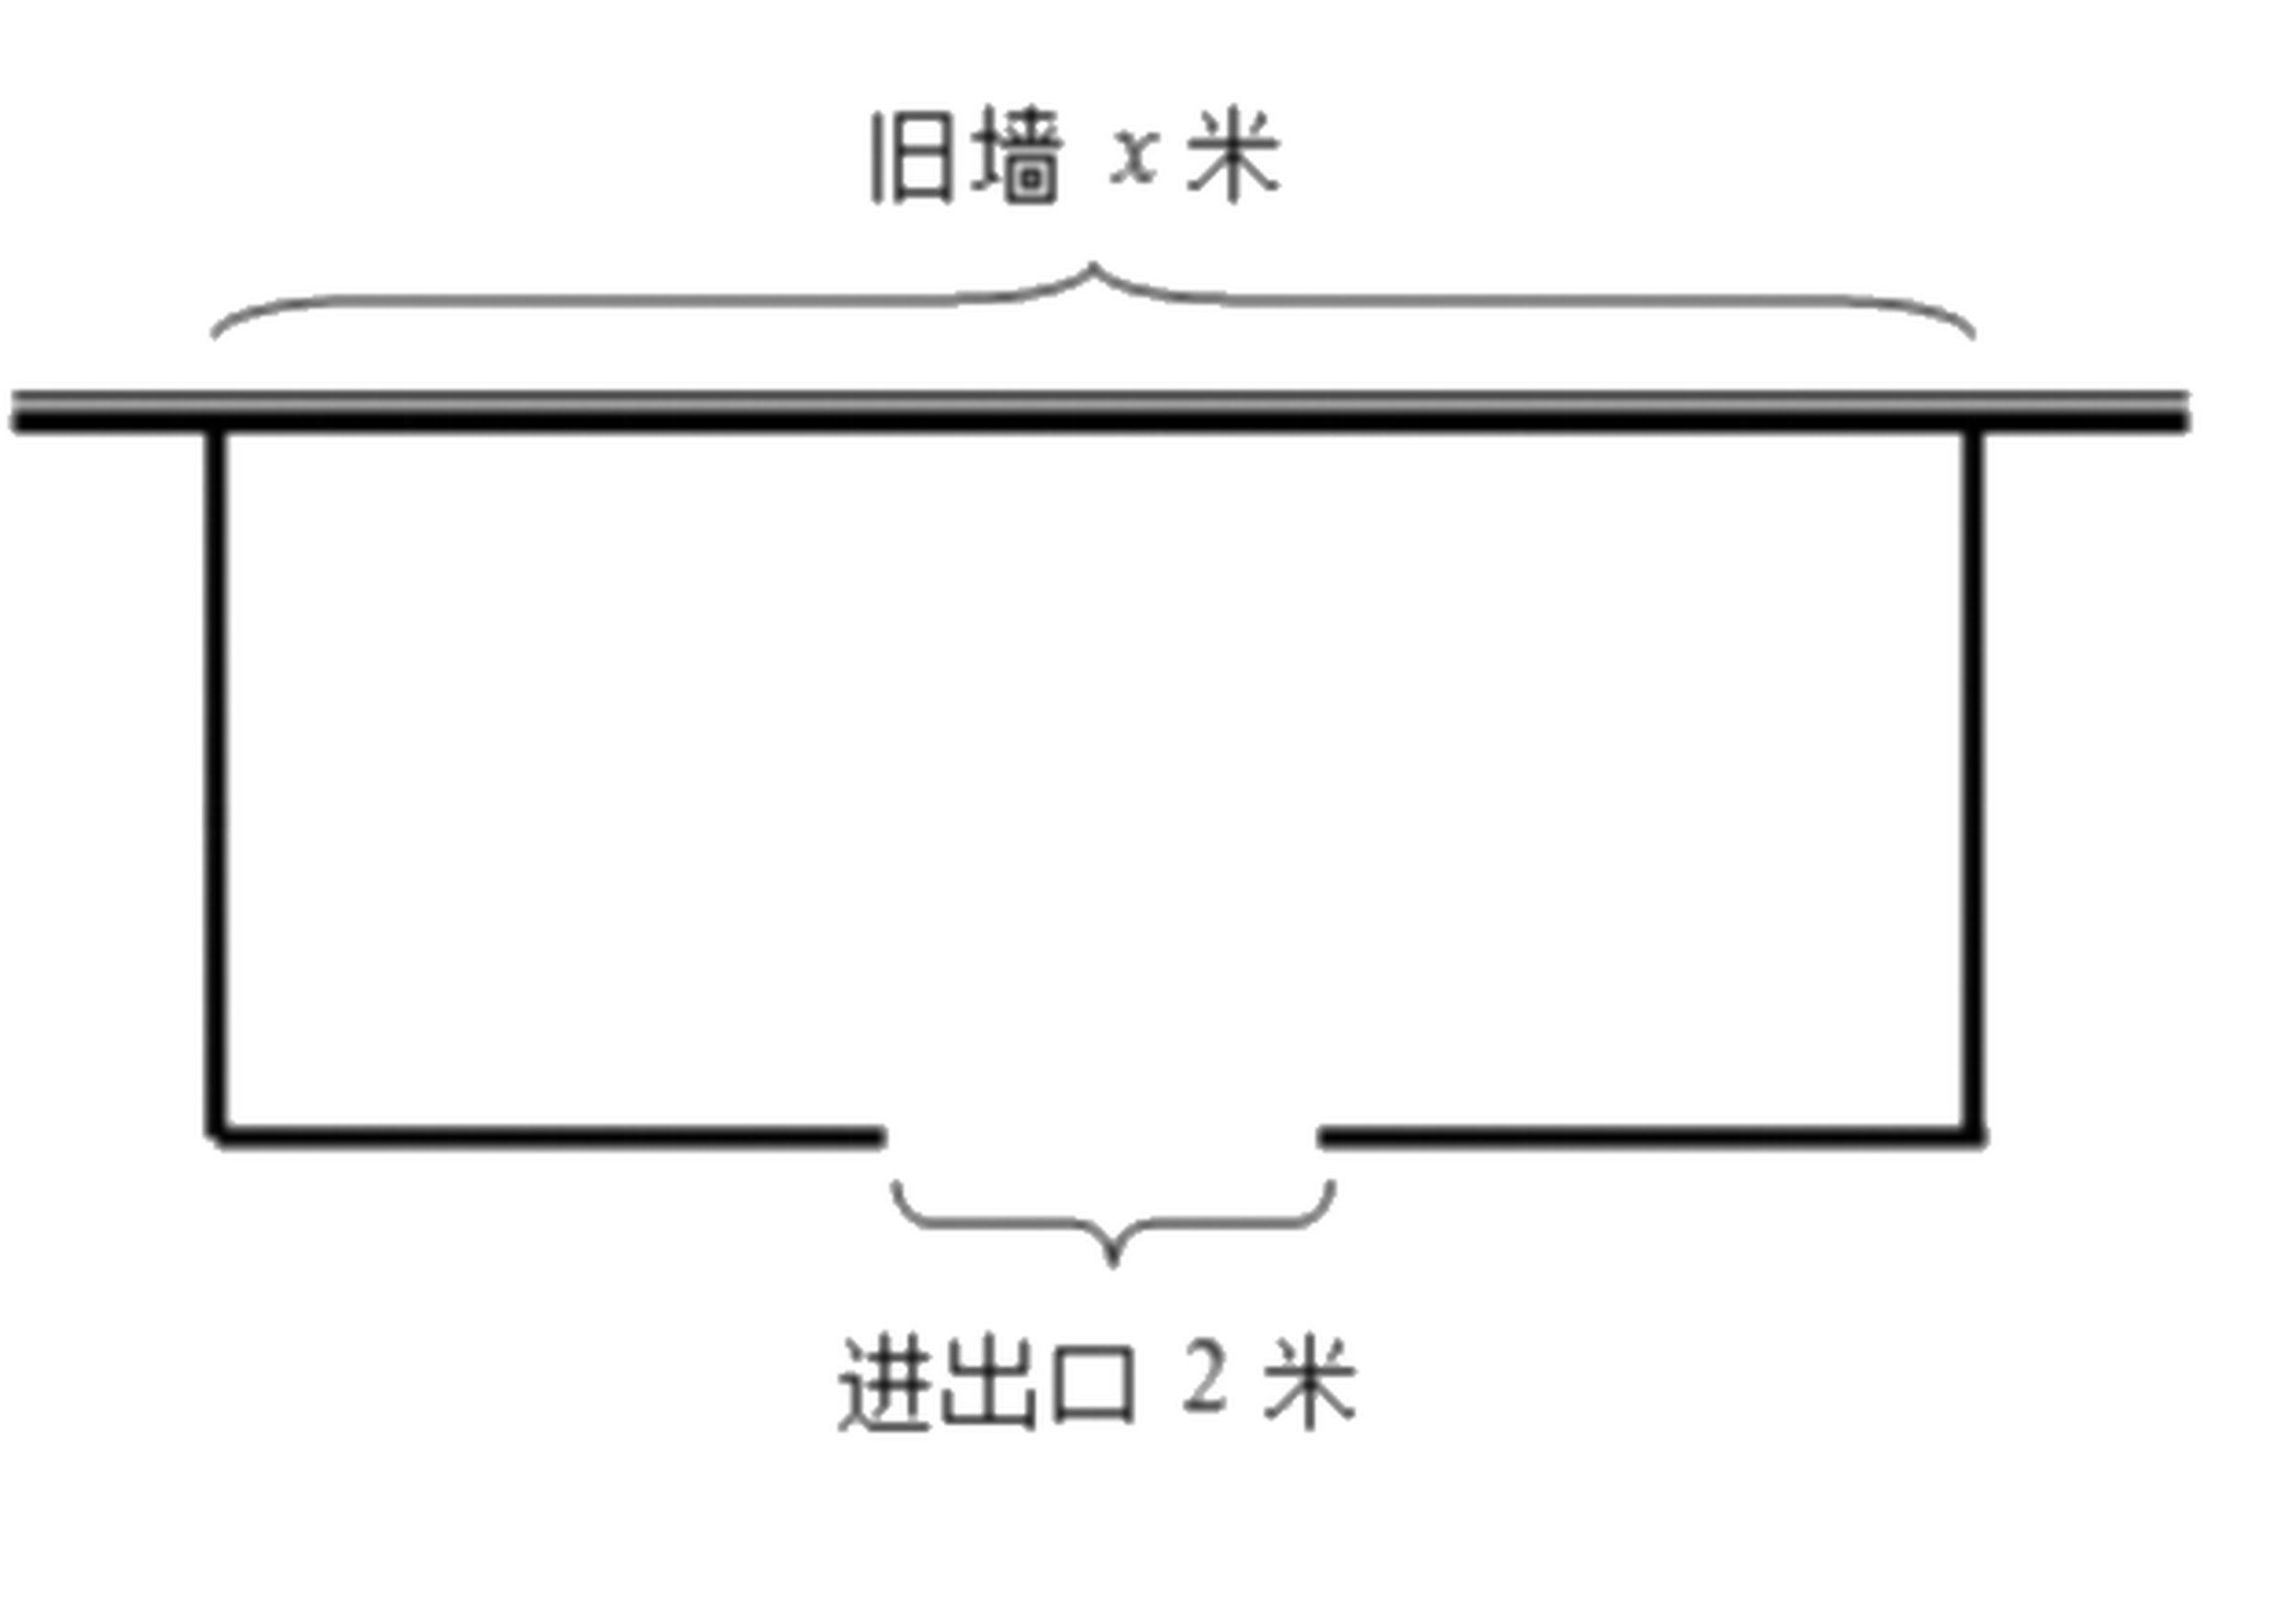
\includegraphics[width=0.60\textwidth]{figures/gao144_q17.png}
\end{center}

(1) 写出总费用 $y$ 关于 $x$ 的表达式;

(2) 试确定 $x$，使修建此矩形场地围墙的总费用最小，并求出最小总费用.

\ifanswer
\solbegin
\step{(1) 设矩形的另一边长为 $a$ 米，}
\step{则 $y=45x+180(x-2)+180\times2a=225x+360a-360$，}
\step{由已知 $xa=360$，得 $a=\dfrac{360}{x}$，所以 $y=225x+\dfrac{360^2}{x}-360(x>0)$;}
\step{(2) 因为 $x>0$，所以 $225x+\dfrac{360^2}{x}\geqslant2\sqrt{225x\cdot\dfrac{360^2}{x}}=10800$，}
\step{所以 $y=225x+\dfrac{360^2}{x}-360\geqslant10440$，}
\step{当且仅当 $225x=\dfrac{360^2}{x}$，即 $x=24$ 时取等号，}
\step{所以当 $x=24$ 米时，修建围墙的总费用最小，最小总费用是 10440 元.}
\solend
\fi

\item 已知集合 $A=\{a_1,a_2,\cdots,a_k\}(k\geqslant2)$，其中 $a_i\in\Z(i=1,2,\cdots,k)$. 定义：若对任意的 $x\in A$，必有 $-x\notin A$，则称集合 $A$ 具有性质 $G$. 由 $A$ 中元素可构成两个点集 $P$ 和 $Q$，$P=\{(x,y)\mid x\in A,y\in A,x+y\in A\}$，$Q=\{(x,y)\mid x\in A,y\in A,x-y\in A\}$，其中 $P$ 有 $m$ 个元素，$Q$ 中有 $n$ 个元素.

(1) 已知集合 $K=\{-1,2,3\}$，判断 $K$ 是否具有性质 $G$; 并写出 $K$ 对应的集合 $P$ 和集合 $Q$;

(2) 若集合 $A=\{1,2,3,4,5,6,7,8,9,10\}$，求对应集合 $Q$ 的元素个数; 一般地，若集合 $A$ 具有性质 $G$，且有 $k$ 个元素，猜测对应的集合 $Q$ 的元素最大个数，并说明理由;

(3) 若集合 $A$ 具有性质 $G$，猜测 $m,n$ 的大小并说明理由.

\ifanswer
\solbegin
\step{(1) 因为 $K=\{-1,2,3\},1,-2,-3$ 都不属于集合 $K$，}
\step{所以集合 $K$ 具有性质 $G$，}
\step{对应集合 $P=\{(-1,3),(3,-1)\},Q=\{(2,-1),(2,3)\}$;}
\step{(2) $A=\{1,2,3,4,5,6,7,8,9,10\}$，则对应集合 $Q$ 中的元素为:}
\step{$(2,1),(3,2),\cdots,(9,8),(10,9)$,}
\step{$(3,1),(4,2),\cdots,(9,7),(10,8)$,}
\step{$(4,1),(5,2),\cdots,(9,6),(10,7)$,}
\step{$\cdots$}
\step{$(9,1),(10,2)$,}
\step{$(10,1)$,}
\step{共有 $9+8+7+\cdots+2+1=45$ 个元素，即对应集合 $Q$ 的元素个数 45;}
\step{集合 $A$ 有 $k$ 个元素，猜测对应的集合 $Q$ 的最大个数为 $\dfrac{k^2-k}{2}$. 理由如下:}
\step{由题意得集合 $A$ 的元素构成有序数对 $(a_i,a_j)(i,j\in\N^*,i\leqslant k,j\leqslant k)$，}
\step{共有 $k^2$ 个，因为 $0\notin A$，所以 $(a_i,a_i)\notin Q$，}
\step{又因为 $a\in A$ 时，$-a\notin A$，所以 $(a_i,a_j)\in Q$ 时，$(a_j,a_i)\notin Q$，}
\step{所以集合 $Q$ 的元素个数为 $\dfrac{k^2-k}{2}$ 个，}
\step{(3) 当集合 $A$ 具有性质 $G$ 时，}
\step{①对于 $(a,b)\in P$，由定义得 $a\in A,b\in A,a+b\in A$，}
\step{又因为集合 $A$ 具有性质 $G$，所以 $(a+b,a)\in Q$，}
\step{如果 $(a,b),(c,d)$ 是 $P$ 中的不同元素，}
\step{那么 $a=c,b=d$ 中至少有一个不成立，}
\step{于是 $b=d,a+b=c+d$ 中至少有一个不成立，}
\step{故 $(a+b,b)$ 和 $(c+d,d)$ 也是 $Q$ 中不同的元素，}
\step{可见 $P$ 的元素个数不多于 $Q$ 的元素个数，即 $m\leqslant n$;}
\step{②对于 $(a,b)\in Q$，由定义得 $a\in A,b\in A,a-b\in A$，}
\step{又因为集合 $A$ 具有性质 $G$，则 $(a-b,b)\in P$，}
\step{如果 $(a,b),(c,d)$ 是 $Q$ 中的不同元素，}
\step{那么 $a=c,b=d$ 中至少有一个不成立，}
\step{于是 $b=d,a-b=c-d$ 中至少有一个不成立，}
\step{故 $(a-b,b)$ 和 $(c-d,d)$ 也是 $P$ 中不同的元素，}
\step{可见 $Q$ 的元素个数不多于 $P$ 的元素个数，即 $n\leqslant m$，}
\step{由①②得 $m=n$.}
\solend
\fi

\end{enumerate}

\end{document}
"
% 紧凑版：xelatex "\def\iscompact{1}% 高一144_风华中学_期中.tex
%   —— 高一上数学"2026-2027 年风华中学高一上期中"（试卷版/答案版/紧凑版）
% 试卷版：xelatex 高一144_风华中学_期中.tex
% 答案版：xelatex "\def\isanswer{1}\input{高一144_风华中学_期中.tex}"
% 紧凑版：xelatex "\def\iscompact{1}\input{高一144_风华中学_期中.tex}"
%
% ① 原始材料：微信公众号"魔都数学加油站"文章，连载"27学年高一144"，原文标题
% "27学年高一144——2026-2027年上海市风华中学高一上期中"；
% 原文链接：https://mp.weixin.qq.com/s/ylUlbXfudWOYC-jlH3jyjw 。
% 正文为 10 张 PNG 页，题目下印【解析】，为讲评版。
% 各页分辨率：01/02/03/05/06/07/09/10 为 2560×3620，04/08 为 4762×6735。
% 题目、解析均据原图转录；卷面粉红色水印"魔都数学加油站"及公众号页脚未录入。
% 全卷插图情况：Q17 有一幅矩形场地示意图（旧墙 x 米 / 进出口 2 米），从 07 页裁出、
%   去粉色水印去色 4× LANCZOS 放大存 figures/gao144_q17.png；其余 9 页逐页通读
%   确认无题目配图、无表格、亦无"题干写如图而源码漏图"一处。
%
% 卷首标题：原卷印作"2026-2027 年风华中学高一上期中"，年份区间按全稿惯例排 en dash；
% 原卷卷面未印副标题，本稿按同期中卷（高一140／141／143）知识模块口径补出
% "集合与常用逻辑用语、不等式、函数"：集合与逻辑见 Q3、Q7、Q9、Q10、Q12、Q16、Q18，
% 不等式见 Q6、Q11、Q13、Q14、Q15、Q17，函数见 Q4、Q5、Q8、Q9。
%
% 题号体例：本卷共 16 题——一、填空题 3—10（8 题）、二、选择题 11—13（3 题）、
% 三、解答题 14—18（5 题）。三节分别 \setcounter{enumi}{2}／{10}／{13}。
% 原卷从第 3 题起、无第 1、2 题，本稿保留原题号；全卷无附加题节。
%
% ② 与原卷的排版差异：
%   ① 原文从第 3 题起，本稿保留原题号；共 16 题三节；
%   ② 原卷 15 题题下印【解析】，唯 Q11 未印【解析】、只把答案"（ BD ）"直接印在
%      题干括号内（放大 04 页 A/B 选项与 05 页 C/D 选项衔接处确认，见 ⑤）；
%      按 高一128／94／106／140 成例：Q11 试卷版括号留空 \mbox{（\quad）}、
%      答案版另提 \ans{$BD$}、不补造原卷没有的解析；其余 15 题印【解析】、
%      括号内一律留空、不另提 \ans{}（Q12 选 C、Q13 选 B 在解析末句"故选 …"）；
%      答案版【答案】/【解析】标记数 = 16（1 个 \ans + 15 个 \solbegin）= 全卷题数；
%      正文 Q11 对应处另有 % 注；
%   ③ 原卷卷面未印副标题，本稿按知识模块口径补出；
%   ④ 原卷填空横线按全稿惯例排 \blankline[4.4em]；选择题括号排 \mbox{（\quad）}，
%      选项段前按惯例加 \keepwithprev；解答题不留作答区、不加 \anspace
%      （原卷为讲评版，与 129／131／132／133／136／140／141／143 同）；
%   ⑤ 数集：Q9 题干与解析"a,b∈R"、Q12 题干"U=R"、Q15 题干"x,y∈R"原卷印
%      斜体或黑板粗体 R，Q18 题干"a_i∈Z"印黑板粗体 Z、Q18 解析"i,j∈N*"印
%      黑板粗体 N，按全稿惯例统一改 \R／\Z／\N^*；绝对值排 \lvert…\rvert，
%      集合描述竖线排 \mid；不等号按全稿惯例排 \leqslant／\geqslant；
%      补集照原卷上划线排 \overline{A}／\overline{B}；空集记号 \varnothing；
%   ⑥ 子题标号 (1)(2)(3) 原卷印半角括号，照录；圈数字 ①② 在正文（文本模式）
%      按原卷照录（Q15、Q18 解析），未进数学式；数学式内半角逗号照录
%      （Q12 解析"$A=(1,2),B=(0,6)$"、Q18 解析"$(a_i,a_j)(i,j\in\N^*,i\leqslant k,j\leqslant k)$"、
%      Q15 解析"$x=1,y=-1$"、Q18 解析"$a=c,b=d$"等，为全稿惯例、非笔误）；
%      全卷行末西文句点照录为 ASCII `.`；行中全角逗号／顿号照录；
%      Q18 解析集合描述中的"或"用 \text{ 或 } 置于数学式内；
%   ⑦ 题干中的中文弯引号按原卷照录（Q3 的" x∈A "／" x∈B "与 Q15 (2) 的命题
%      引号，含引号内空格），注释内一律 ASCII 引号；
%   ⑧ Q17 配图：题干写"如图所示"，配图居中排在题干之后、子问之前，三版都出；
%      在 Q17 \item 之前加 \needvspace{10cm} 把"题干＋图"整块推走。Q17 是
%      "三、解答题"节内第 4 题（非节首题），故守卫放在 \item 之前而非 \bigsec
%      之前不会让节标题孤落页末（B 类）；三版切页审计均"合计异常：无"；
%   ⑨ 跨页续印按题合并：Q3 在 01 页；Q4/5/6 在 01 页（Q6 解析续到 02 页顶）；
%      Q7/8/9 在 02 页（Q9 题干跨 02→03）；Q10 在 03 页、解析跨 03→04（很长，
%      按余数分组 A₁/A₂/A₃）；Q11 在 04 页（"二、选择题"节标题也在 04 页下部）、
%      Q12/13 在 05 页（"三、解答题"标题在 05 页下部）；Q14 在 05 页末、解析在 06 页；
%      Q15/16 在 06 页（Q16 续到 07 页）；Q17 在 07 页；Q18 在 08 页、解析跨
%      08/09/10 页（性质 G 压轴，3 问，很长）；本稿按题连排，不丢行、不并折行；
%   ⑩ Q8 解析"法一：""法二："两处标签经放大 02 页逐字确认原卷均印红色
%      （见 ⑤）；按全稿惯例（高一53 成例）不引入红色、均照录为黑体着色
%      \stepm{法一：}{…}／\stepm{法二：}{…}，不改 common.sty；
%      文件头在此注明原卷为红色；
%   ⑪ "图像／图象"逐处核：全卷未出现"图像"或"图象"字样，无统一问题；
%   ⑫ \left…\right 不得拆到不同 $…$ 组；cases 块整体算一个印刷行；
%      Q4 分式与 8×(-3/4) 同一 $…$ 组，Q13 的 \left(\frac1x+\frac2y\right) 同理。
%
% ③ 行数复核：一条 \step／\stepm 行 = 原卷解析的一个印刷行，cases 块作一个印刷行计。
%   逐题数（含 \stepm）：Q3：3；Q4：1；Q5：1；Q6：5；Q7：4；Q8：8（6 \step
%   ＋ 2 \stepm，法一/法二标签各占 1 行）；Q9：6；Q10：23；Q11：0（原卷无解析，
%   答案另提 \ans{$BD$}）；Q12：5；Q13：3；Q14：5；Q15：8；Q16：7；Q17：7；
%   Q18：32。合计 116 条 \step ＋ 2 条 \stepm ＝ 118 个印刷行，与原卷逐题相等。
%   全卷 15 题设 \solbegin…\solend ＋ Q11 一处 \ans{}，答案版【答案】/【解析】
%   标记数 = 16 = 全卷题数。
%
% ④ 判别式／子集符号结论（逐处放大原图照录、不得统一）：
%   判别式全卷 2 处，逐页放大扫过 10 页确认（Q4 为分式指数化简、不含判别式）：
%     · Q9【解析】"所以 △=a^2-4b=0" 原卷印细线、扁等边三角（宽≈高、笔画细，
%       放大见 /tmp/gao144fh/z_q9_tri.png、z_tri_Q9.png），照录 \triangle；
%     · Q15 (2)【解析】cases 块"Δ=(a-2)^2-4(a-2)≤0" 原卷印等腰偏高、粗笔画
%       三角（高>宽，放大见 z_q15_tri.png、z_tri_Q15.png），照录 \Delta；
%   两形不同、全卷混用，逐处照录不统一（参照 高一142 头注④口径）。
%   子集符号全卷 4 处，逐处放大核：
%     · Q3 解析"所以 B⊆A"、Q16 (1) 解析"所以 B⊆A" 原卷均印带下划线的 ⊆
%       （z_q3_symbol.png、z_q16_subset2.png），照录 \subseteq；
%     · Q12 选项 B"$\overline{A}\subset B$" 原卷印单线 ⊂（z_q12_opts2.png），
%       照录 \subset；Q12 解析"$\overline{A}=(-\infty,1]\cup[2,+\infty)\not\subset B$"
%       原卷印单线带斜杠 ⊄（z_q12_notsym3.png），照录 \not\subset；
%   \subset 与 \subseteq 混用，逐处照录不统一。补集照原卷上划线 \overline{A}／
%   \overline{B}，空集 \varnothing，数集 \R／\Z／\N^* 归一见 ② ⑤。
%
% ⑤ 存疑／特殊体例（主会话逐处放大原图复核确认，照录未改，正文对应处另有 % 注）：
%   1. 第 11 题原卷把答案"（ BD ）"直接印在题干括号内、题下未印【解析】
%      （放大 04 页 A/B 选项与 05 页 C/D 选项衔接处确认：05 页顶 C/D 选项后
%      直接接第 12 题）。按 高一128／94／106／140 成例括号留空、另提
%      \ans{$BD$}，不补造解析（不编造）。
%   2. 第 10 题题干"集合 $S$ 为集合 $M=\{1,2,3,4,\cdots,2026\}$，的子集"在
%      集括号与"的子集"之间原卷多印一个全角逗号（放大 03 页确认），
%      按存疑照录未删，正文对应处另有 % 注。
%   3. 第 8 题解析"法一：""法二："两处原卷均印红色（放大 02 页逐字确认），
%      按全稿惯例不引入红色、两处均照录为黑体着色 \stepm（见 ② ⑩）。
%   全卷除此 3 条外未发现其它笔误／自相矛盾处。
%
% ⑥ 跨页续印按题合并说明：见 ② ⑨。
%
\documentclass[a4paper,11pt]{article}
\usepackage{common}

\begin{document}

\examtitlest[3]{2026--2027 年风华中学高一上期中}{集合与常用逻辑用语、不等式、函数}

\bigsec{一、填空题}

\begin{enumerate}
\setcounter{enumi}{2}

\item $A=\{x\mid x>4\}$，$B=\{x\mid x>a\}$，若命题 “ $x\in A$ ” 是命题 “ $x\in B$ ” 的必要条件，则 $a$ 的取值范围是\blankline[4.4em].

\ifanswer
\solbegin
\step{因为 “ $x\in A$ ” 是命题 “ $x\in B$ ” 的必要条件，所以 $B\subseteq A$，}% 子集符号原卷印带下划线 $\subseteq$，照录
\step{因为 $A=\{x\mid x>4\}$，$B=\{x\mid x>a\}$，所以 $a\geqslant4$，}
\step{所以 $a$ 的取值范围是 $\{a\mid a\geqslant4\}$.}
\solend
\fi

\item 已知 $a>0,b>0$，化简式子：$\dfrac{8a^{\frac34}b^3}{\left(a^{\frac16}b^{\frac32}\right)\left(-\dfrac43 a^{\frac1{12}}b^{\frac12}\right)}=$\blankline[4.4em].

\ifanswer
\solbegin
\step{$\dfrac{8a^{\frac34}b^3}{\left(a^{\frac16}b^{\frac32}\right)\left(-\dfrac43 a^{\frac1{12}}b^{\frac12}\right)}=8\times\left(-\dfrac34\right)a^{\frac34-\frac16-\frac1{12}}b^{3-\frac32-\frac12}=-6a^{\frac12}b=-6b\sqrt a$.}
\solend
\fi

\item 已知 $\lg2=a$，$\lg3=b$，则 $\log_5 6=$\blankline[4.4em]（结果用 $a,b$ 表示）.

\ifanswer
\solbegin
\step{$\log_5 6=\dfrac{\lg6}{\lg5}=\dfrac{\lg2+\lg3}{1-\lg2}=\dfrac{a+b}{1-a}$.}
\solend
\fi

\item 若关于 $x$ 的不等式 $ax>b$ 的解集为 $(-\infty,2)$，则不等式 $bx+a>0$ 的解集为\blankline[4.4em].

\ifanswer
\solbegin
\step{因为不等式 $ax>b$ 的解集为 $(-\infty,2)$，所以 $a<0$，}
\step{所以由不等式解得 $x<\dfrac ba$，所以 $\dfrac ba=2$，即 $b=2a$，}
\step{代入不等式 $bx+a>0$，得 $2ax+a>0$，}
\step{因为 $a<0$，所以不等式化为 $2x+1<0$，解得 $x<-\dfrac12$，}
\step{故不等式的解集为 $\left(-\infty,-\dfrac12\right)$.}
\solend
\fi

\item 如果集合 $A=\{x\mid x^2-4x\leqslant0\}$，$B=\{x\mid x^2+ax+b\leqslant0\}$，$A\cap B=\{x\mid3\leqslant x\leqslant4\}$，$A\cup B=\{x\mid0\leqslant x\leqslant5\}$，则 $a+b=$\blankline[4.4em].

\ifanswer
\solbegin
\step{由题意得 $A=\{x\mid x^2-4x\leqslant0\}=[0,4]$，}
\step{又因为 $A\cap B=\{x\mid3\leqslant x\leqslant4\}$，$A\cup B=\{x\mid0\leqslant x\leqslant5\}$，}
\step{所以 $B=\{x\mid3\leqslant x\leqslant5\}$，即方程 $x^2+ax+b=0$ 的两根为 $3,5$，}
\step{由韦达定理得 $\begin{cases}3+5=-a\\3\times5=b\end{cases}$，解得 $a=-8$，$b=15$，所以 $a+b=15-8=7$.}
\solend
\fi

% 第 8 题：原卷"法一：""法二："两处标签均印红色（8× 放大确认）；按交办口径
% "法一"用普通 \step、"法二："排 \stepm（加粗着色、不引红色），见头注 ② ⑩／⑤
\item 若关于 $x$ 的方程 $\lvert x-1\rvert+\lvert\pi-x\rvert=\pi-1$ 的解集为\blankline[4.4em].

\ifanswer
\solbegin
\stepm{法一：}{因为 $\lvert x-1\rvert+\lvert\pi-x\rvert=\begin{cases}x-1+x-\pi,x\geqslant\pi\\\pi-1,1<x<\pi\\1-x+\pi-x,x\leqslant1\end{cases}=\begin{cases}2x-1-\pi,x\geqslant\pi\\\pi-1,1<x<\pi\\1+\pi-2x,x\leqslant1\end{cases}$.}
\step{当 $x\geqslant\pi$ 时，令 $2x-1-\pi=\pi-1$，得 $x=\pi$；}
\step{当 $1<x<\pi$ 时，$\lvert x-1\rvert+\lvert\pi-x\rvert=\pi-1$ 恒成立；}
\step{当 $x\leqslant1$ 时，令 $1+\pi-2x=\pi-1$，得 $x=1$.}
\step{综上所述，方程 $\lvert x-1\rvert+\lvert\pi-x\rvert=\pi-1$ 的解集为 $[1,\pi]$.}
\stepm{法二：}{因为 $\lvert x-1\rvert+\lvert\pi-x\rvert\geqslant\lvert x-1+\pi-x\rvert=\pi-1$，}
\step{当且仅当 $(x-1)(\pi-x)\geqslant0$ 时取等号，}
\step{故方程 $\lvert x-1\rvert+\lvert\pi-x\rvert=\pi-1$ 的解集为 $[1,\pi]$.}
\solend
\fi

% 第 9 题：题干跨 02→03 页；解析判别式原卷印细线扁等边三角 $\triangle$，照录
\item 已知函数 $f(x)=x^2+ax+b(a,b\in\R)$ 和 $x$ 轴有且只有一个交点，若关于 $x$ 的不等式 $f(x)<c$ 的解集为 $(m,m+6)$，则 $c=$\blankline[4.4em].

\ifanswer
\solbegin
\step{因为函数 $f(x)=x^2+ax+b(a,b\in\R)$ 和 $x$ 轴有且只有一个交点，}
\step{所以 $\triangle=a^2-4b=0$，即 $b=\dfrac{a^2}{4}$，}% 判别式原卷印扁等边三角 $\triangle$，照录
\step{不等式 $f(x)<c$ 的解集为 $(m,m+6)$，}
\step{即 $x^2+ax+\dfrac{a^2}{4}-c<0$ 的解集为 $(m,m+6)$，}
\step{所以方程 $x^2+ax+\dfrac{a^2}{4}-c=0$ 的两个根为 $x_1=m$，$x_2=m+6$，}
\step{所以 $\begin{cases}x_1+x_2=2m+6=-a\\x_1x_2=m(m+6)=\dfrac{a^2}{4}-c\end{cases}$，消去 $m$ 得 $\dfrac{a^2}{4}-9=\dfrac{a^2}{4}-c$，解得 $c=9$.}
\solend
\fi

% 第 10 题：原卷题干在集括号与"的子集"之间多印一个全角逗号，照录未改（存疑，见头注 ⑤）
\item 已知集合 $S$ 为集合 $M=\{1,2,3,4,\cdots,2026\}$，的子集，并且集合 $S$ 中任意两个元素之和不能被 3 整除，则集合 $S$ 中元素个数的最大值为\blankline[4.4em].

\ifanswer
\solbegin
\step{对于集合 $M=\{1,2,3,4,\cdots,2026\}$，}
\step{所有被 3 除余数为 0 的元素组成的集合为 $A_3=\{3,6,9,\cdots,2025\}$，}
\step{元素个数为 675;}
\step{所有被 3 除余数为 1 的元素组成的集合为 $A_1=\{1,4,7,\cdots,2026\}$，}
\step{元素个数为 676;}
\step{所有被 3 除余数为 2 的元素组成的集合为 $A_2=\{2,5,8,\cdots,2024\}$，}
\step{元素个数为 675;}
\step{集合 $S$ 中任意两个元素之和不能被 3 整除，}
\step{若两个元素分别来自 $A_1$ 和 $A_2$，则两数之和除以 3 的余数为 $1+2=3\equiv0$，}
\step{即和能被 3 整除，}
\step{所以 $S$ 不能同时包含 $A_1$ 和 $A_2$ 中的元素，}
\step{即 $S$ 最多只能选取 $A_1$、$A_2$ 一个集合中的全部元素;}
\step{若两个元素都来自 $A_3$，则两数之和除以 3 的余数为 $0+0=0$，即和能被 3 整除，}
\step{所以 $S$ 中最多包含 $A_3$ 中的 1 个元素;}
\step{对 $A_1$ 内的任意两个元素，其和除以 3 的余数为 $1+1=2$，不能被 3 整除;}
\step{$A_1$ 中元素与 $A_3$ 中元素的和除以 3 余数为 $1+0=1$，不能被 3 整除，}
\step{所以 $A_1$ 的全部元素与 $A_3$ 中的任意 1 个元素的组合满足题意;}
\step{对 $A_2$ 内的任意两个元素，其和除以 3 的余数为 $2+2=4\equiv1$，不能被 3 整除;}
\step{$A_2$ 中元素与 $A_3$ 中元素的和除以 3 的余数为 $2+0=2$，不能被 3 整除，}
\step{所以 $A_2$ 的全部元素与 $A_3$ 中任意 1 个元素的组合也满足题意.}
\step{故若选取 $A_2$ 全部元素加 1 个 $A_3$ 元素，总个数为 $675+1=676$;}
\step{选取 $A_1$ 全部元素加 1 个 $A_3$ 元素，总个数为 $676+1=677$;}
\step{所以集合 $S$ 中元素个数的最大值为 677.}
\solend
\fi

\end{enumerate}

\bigsec{二、选择题}

\begin{enumerate}
\setcounter{enumi}{10}

% 第 11 题：原卷把答案"（ BD ）"直接印在题干括号内、题下无【解析】（放大 04 页 A/B 选项
% 与 05 页 C/D 选项衔接处确认）。按 高一128／94／106／140 成例：试卷版括号留空、
% 答案版另提 \ans{$BD$}、不补造原卷没有的解析（不编造）。
\item 已知实数 $a,b$，下列四个不等式中正确的是\mbox{（\quad）}

\keepwithprev
A. $a+\dfrac1a\geqslant2$\qquad B. $\sqrt{a^2+2}+\dfrac{1}{\sqrt{a^2+2}}\geqslant2$

C. $\dfrac{a+b}{2}\leqslant\sqrt{ab}$\qquad D. $a^2+b^2\geqslant2ab$

\ifanswer
\ans{$BD$}
\fi

\item 若全集 $U=\R$，$A=\{x\mid x^2-3x+2<0\}$，$B=\{x\mid0<x<6\}$，则\mbox{（\quad）}

\keepwithprev
A. $A\cap B=B$\qquad B. $\overline{A}\subset B$\qquad C. $A\cap\overline{B}=\varnothing$\qquad D. $A\cup B=A$

\ifanswer
\solbegin
\step{由 $x^2-3x+2<0$，则 $A=(1,2),B=(0,6)$，所以 $A\cap B=(1,2)=A,A$ 错误;}
\step{$\overline{A}=(-\infty,1]\cup[2,+\infty)\not\subset B$，$B$ 错误;}
\step{$\overline{B}=(-\infty,0]\cup[6,+\infty)$，所以 $A\cap\overline{B}=\varnothing,C$ 正确;}
\step{$A\cup B=(0,6)\ne A,D$ 错误.}
\step{故选 $C$.}
\solend
\fi

\item 已知正数 $x$、$y$ 满足 $\dfrac1x+\dfrac2y=1$，不等式 $3x+2y-1>m$ 恒成立，则实数 $m$ 的取值范围是\mbox{（\quad）}

\keepwithprev
A. $(-\infty,4+6\sqrt2)$\qquad B. $(-\infty,6+4\sqrt3)$\qquad C. $(6+4\sqrt2,+\infty)$\qquad D. $(8+4\sqrt3,+\infty)$

\ifanswer
\solbegin
\step{$3x+2y=(3x+2y)\left(\dfrac1x+\dfrac2y\right)=7+\dfrac{6x}{y}+\dfrac{2y}{x}\geqslant7+2\sqrt{\dfrac{6x}{y}\cdot\dfrac{2y}{x}}=7+4\sqrt3$，}
\step{当且仅当 $\dfrac{6x}{y}=\dfrac{2y}{x}$，即 $y=\sqrt3x=\sqrt3+2$ 时取等号，}
\step{故要使原式成立，只需 $m<6+4\sqrt3$. 故选 $B$.}
\solend
\fi

\end{enumerate}

\bigsec{三、解答题}

\begin{enumerate}
\setcounter{enumi}{13}

\item 解关于 $x$ 的不等式：

(1) $x^2-2\lvert x\rvert-3>0$；

(2) $\dfrac{2x-1}{x+2}<1$.

\ifanswer
\solbegin
\step{(1) 原不等式等价于 $(\lvert x\rvert-3)(\lvert x\rvert+1)>0$，}
\step{$\lvert x\rvert+1>0$，故 $\lvert x\rvert>3$，解得 $x<-3$ 或 $x>3$，}
\step{故不等式的解集为 $(-\infty,-3)\cup(3,+\infty)$.}
\step{(2) 已知 $\dfrac{2x-1}{x+2}<1$，则 $\dfrac{2x-1}{x+2}-1<0$，即 $\dfrac{x-3}{x+2}<0$，}
\step{等价于 $(x-3)(x+2)<0$，解得 $-2<x<3$，故不等式的解集为 $(-2,3)$.}
\solend
\fi

\item (1) 已知 $x,y\in\R$，比较 $x^2+y^2$ 与 $2x-2y-2$ 的大小.

(2) “不等式 $(a-2)x^2+(a-2)x+1\geqslant0$ 对一切实数恒成立” 是假命题，求实数 $a$ 的取值范围.

\ifanswer
\solbegin
\step{(1) $x^2+y^2-(2x-2y-2)=x^2+y^2-2x+2y+2=(x-1)^2+(y+1)^2\geqslant0$，}
\step{故 $x^2+y^2\geqslant2x-2y-2$，当且仅当 $x=1,y=-1$ 时取等号.}
\step{(2) 先求命题 “$(a-2)x^2+(a-2)x+1\geqslant0$ 对一切实数恒成立” 为真，}
\step{①当 $a-2=0$ 时，即 $a=2$，不等式化为 $1\geqslant0$，成立，符合条件，}
\step{②当 $a-2\ne0$ 时，则 $\begin{cases}a-2>0\\\Delta=(a-2)^2-4(a-2)\leqslant0\end{cases}$，解得 $2<a\leqslant6$，}% 判别式原卷印等腰偏高三角 $\Delta$，照录
\step{综上①②，命题为真时 $2\leqslant a\leqslant6$，}
\step{该命题为假命题，则 $a<2$ 或 $a>6$，}
\step{所以实数 $a$ 的取值范围是 $(-\infty,2)\cup(6,+\infty)$.}
\solend
\fi

\item 设集合 $A=\{x\mid-1\leqslant x\leqslant2\}$，$B=\{x\mid m-1<x<2m+1\}$.

(1) 若 $A\cup B=A$，求实数 $m$ 的取值范围;

(2) 若 $B\cap\overline{A}$ 中只有一个整数 $-2$，求实数 $m$ 的取值范围.

\ifanswer
\solbegin
\step{(1) 因为 $A\cup B=A$，所以 $B\subseteq A$，}% 子集符号原卷印带下划线 $\subseteq$，照录
\step{当 $B=\varnothing$ 时，有 $m-1\geqslant2m+1$，解得 $m\leqslant-2$；}
\step{当 $B\ne\varnothing$ 时，有 $\begin{cases}m-1<2m+1\\m-1\geqslant-1\\2m+1\leqslant2\end{cases}$，解得 $0\leqslant m\leqslant\dfrac12$，}
\step{所以实数 $m$ 的取值范围是 $(-\infty,-2]\cup\left[0,\dfrac12\right]$;}
\step{(2) 由集合 $A=\{x\mid-1\leqslant x\leqslant2\}$，得 $\overline{A}=\{x\mid x<-1\text{ 或 }x>2\}$，}
\step{若 $B\cap\overline{A}$ 中只有一个整数 $-2$，则 $B\ne\varnothing$，且满足 $\begin{cases}m-1<2m+1\\-3\leqslant m-1<-2\\-2<2m+1\leqslant3\end{cases}$}
\step{解得 $-\dfrac32<m<-1$，所以实数 $m$ 的取值范围是 $\left(-\dfrac32,-1\right)$.}
\solend
\fi

% 第 17 题配图是"题干＋图"整块；守卫放在 \item 之前（Q17 非节首题，不会让节标题孤落页末）
\needvspace{10cm}
\item 现要围建一个面积为 360 平方米的矩形场地，要求矩形场地的一面利用旧墙（利用旧墙需维修），其它三面围墙要新建，在旧墙的对面的新墙上要留一个宽度为 2 米的进出口，如图所示，已知旧墙的维修费用为 45 元/米，新墙的造价为 180 元/米，设利用的旧墙的长度为 $x$ 米，工程总造价为 $y$（单位：元）.

\begin{center}
% 矩形场地示意图取自 07 页右侧，去粉色水印、去色、4× LANCZOS 放大
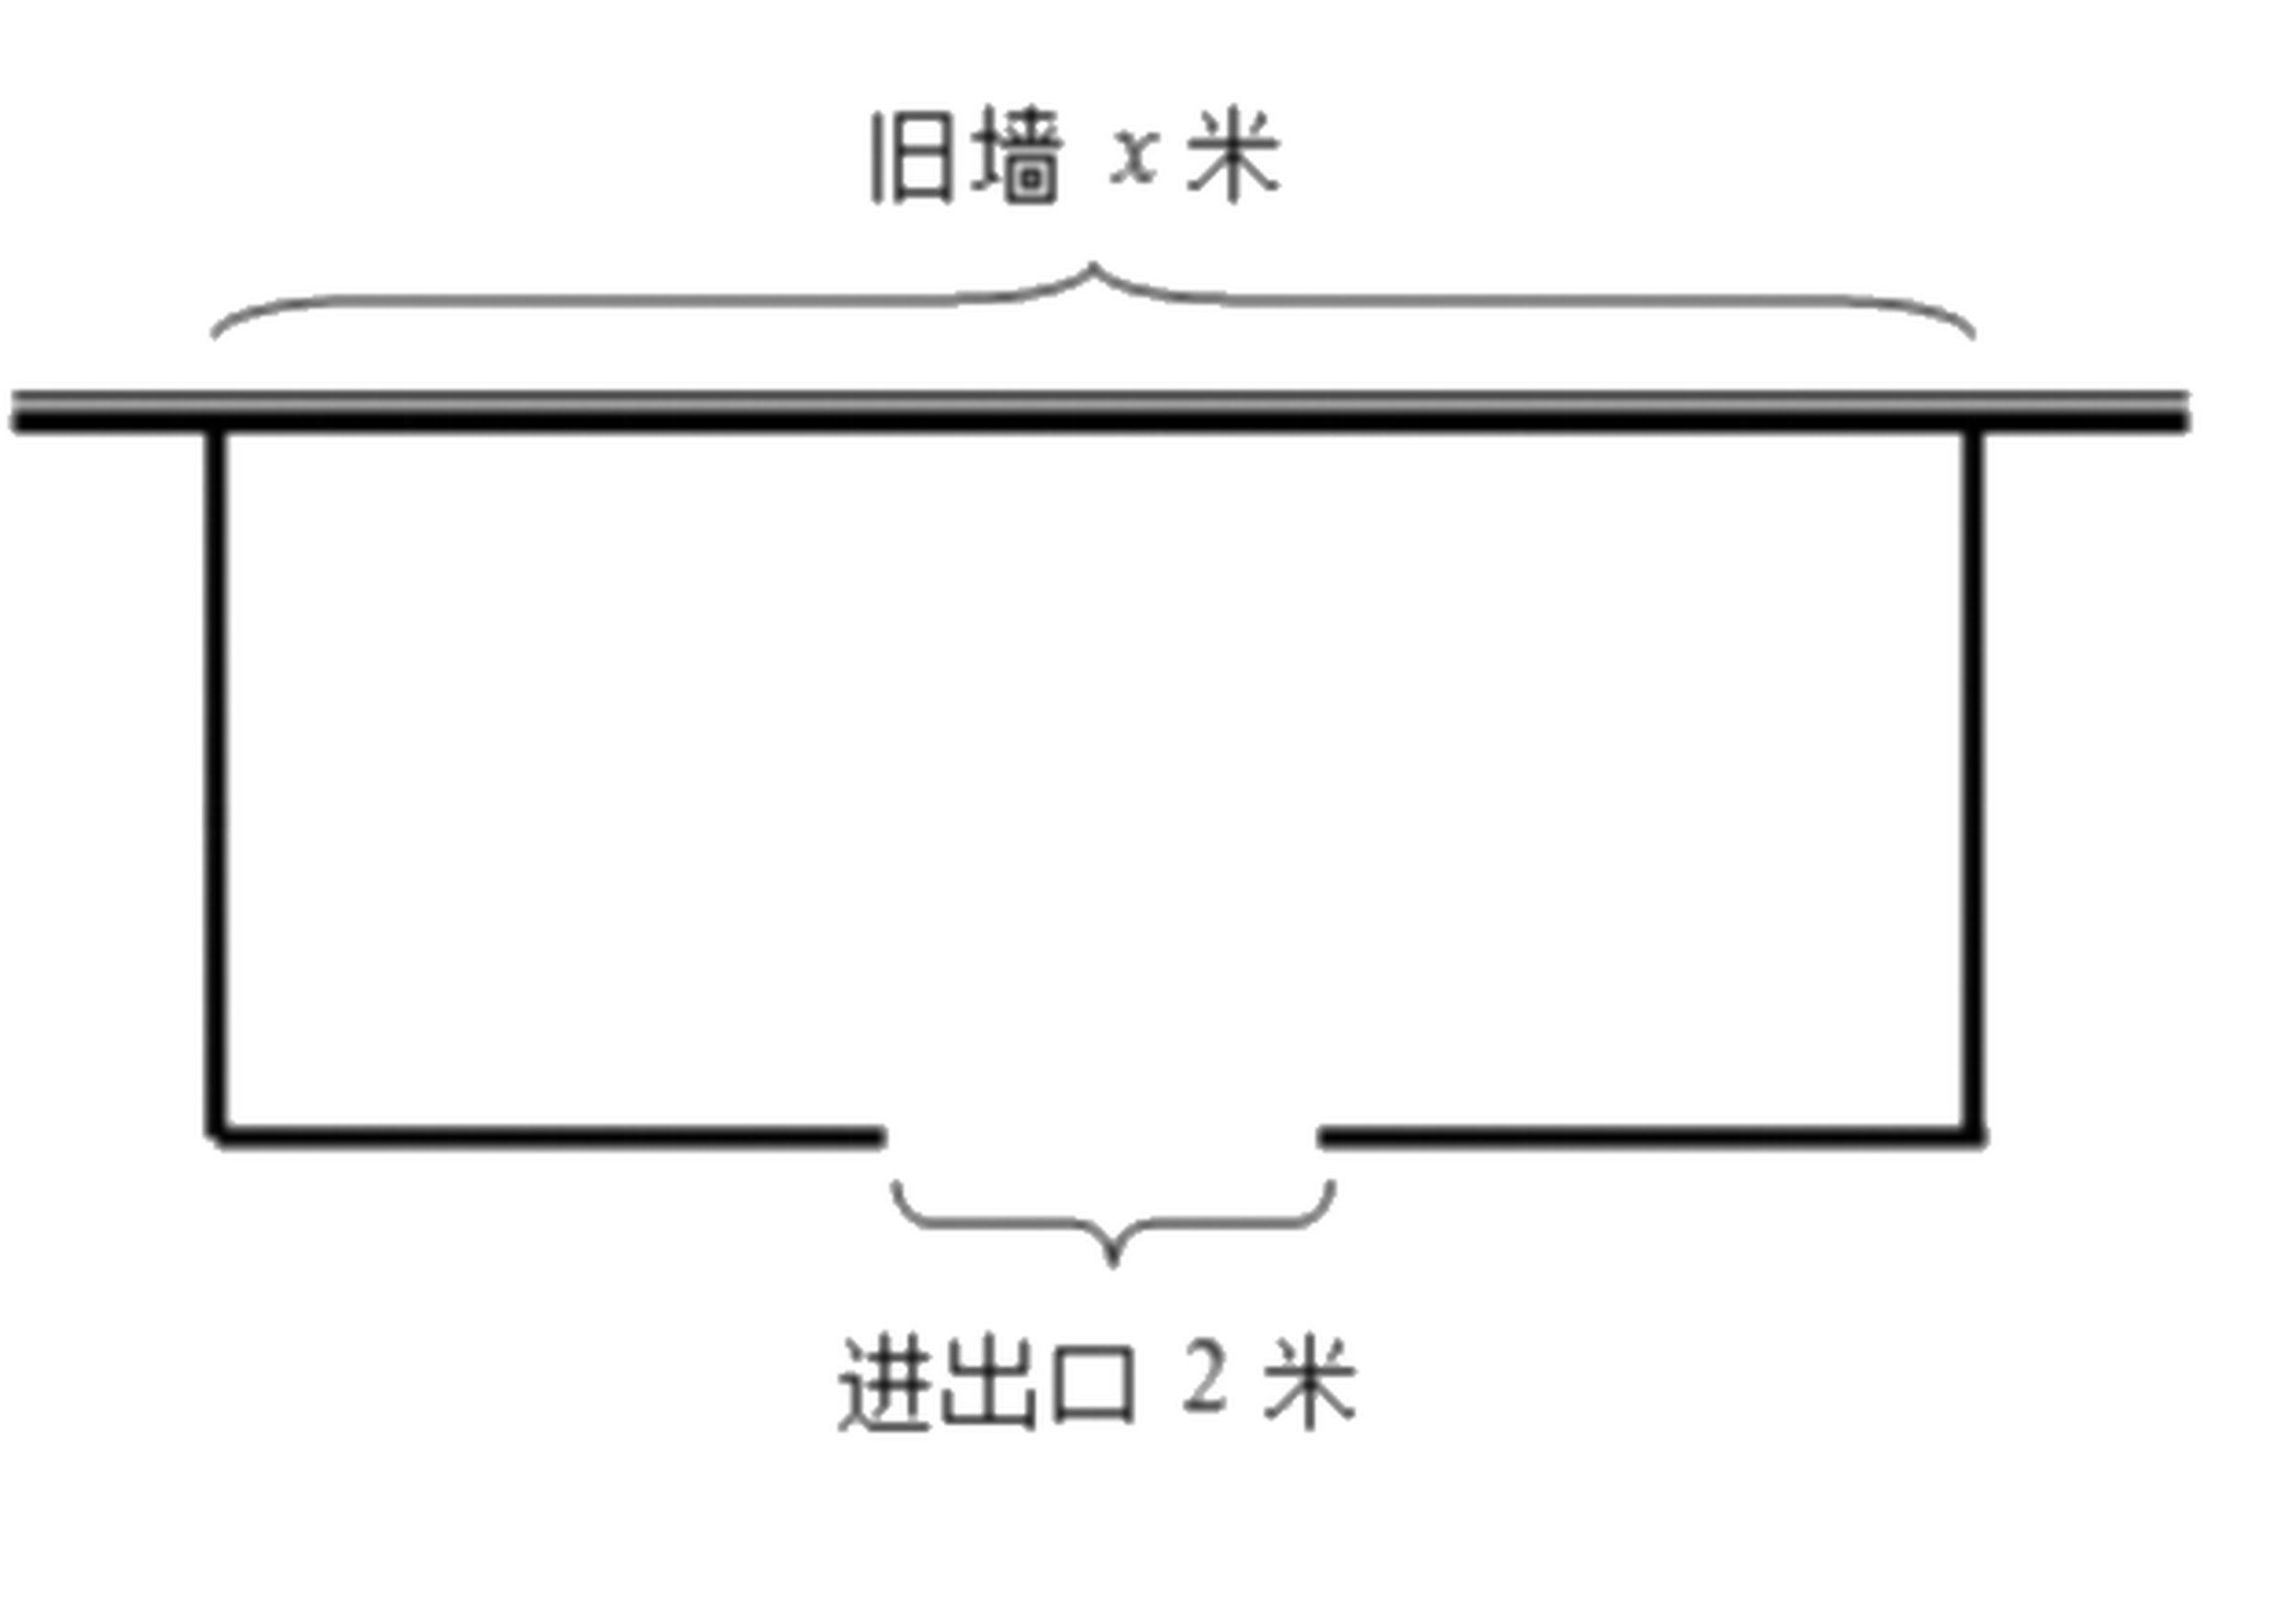
\includegraphics[width=0.60\textwidth]{figures/gao144_q17.png}
\end{center}

(1) 写出总费用 $y$ 关于 $x$ 的表达式;

(2) 试确定 $x$，使修建此矩形场地围墙的总费用最小，并求出最小总费用.

\ifanswer
\solbegin
\step{(1) 设矩形的另一边长为 $a$ 米，}
\step{则 $y=45x+180(x-2)+180\times2a=225x+360a-360$，}
\step{由已知 $xa=360$，得 $a=\dfrac{360}{x}$，所以 $y=225x+\dfrac{360^2}{x}-360(x>0)$;}
\step{(2) 因为 $x>0$，所以 $225x+\dfrac{360^2}{x}\geqslant2\sqrt{225x\cdot\dfrac{360^2}{x}}=10800$，}
\step{所以 $y=225x+\dfrac{360^2}{x}-360\geqslant10440$，}
\step{当且仅当 $225x=\dfrac{360^2}{x}$，即 $x=24$ 时取等号，}
\step{所以当 $x=24$ 米时，修建围墙的总费用最小，最小总费用是 10440 元.}
\solend
\fi

\item 已知集合 $A=\{a_1,a_2,\cdots,a_k\}(k\geqslant2)$，其中 $a_i\in\Z(i=1,2,\cdots,k)$. 定义：若对任意的 $x\in A$，必有 $-x\notin A$，则称集合 $A$ 具有性质 $G$. 由 $A$ 中元素可构成两个点集 $P$ 和 $Q$，$P=\{(x,y)\mid x\in A,y\in A,x+y\in A\}$，$Q=\{(x,y)\mid x\in A,y\in A,x-y\in A\}$，其中 $P$ 有 $m$ 个元素，$Q$ 中有 $n$ 个元素.

(1) 已知集合 $K=\{-1,2,3\}$，判断 $K$ 是否具有性质 $G$; 并写出 $K$ 对应的集合 $P$ 和集合 $Q$;

(2) 若集合 $A=\{1,2,3,4,5,6,7,8,9,10\}$，求对应集合 $Q$ 的元素个数; 一般地，若集合 $A$ 具有性质 $G$，且有 $k$ 个元素，猜测对应的集合 $Q$ 的元素最大个数，并说明理由;

(3) 若集合 $A$ 具有性质 $G$，猜测 $m,n$ 的大小并说明理由.

\ifanswer
\solbegin
\step{(1) 因为 $K=\{-1,2,3\},1,-2,-3$ 都不属于集合 $K$，}
\step{所以集合 $K$ 具有性质 $G$，}
\step{对应集合 $P=\{(-1,3),(3,-1)\},Q=\{(2,-1),(2,3)\}$;}
\step{(2) $A=\{1,2,3,4,5,6,7,8,9,10\}$，则对应集合 $Q$ 中的元素为:}
\step{$(2,1),(3,2),\cdots,(9,8),(10,9)$,}
\step{$(3,1),(4,2),\cdots,(9,7),(10,8)$,}
\step{$(4,1),(5,2),\cdots,(9,6),(10,7)$,}
\step{$\cdots$}
\step{$(9,1),(10,2)$,}
\step{$(10,1)$,}
\step{共有 $9+8+7+\cdots+2+1=45$ 个元素，即对应集合 $Q$ 的元素个数 45;}
\step{集合 $A$ 有 $k$ 个元素，猜测对应的集合 $Q$ 的最大个数为 $\dfrac{k^2-k}{2}$. 理由如下:}
\step{由题意得集合 $A$ 的元素构成有序数对 $(a_i,a_j)(i,j\in\N^*,i\leqslant k,j\leqslant k)$，}
\step{共有 $k^2$ 个，因为 $0\notin A$，所以 $(a_i,a_i)\notin Q$，}
\step{又因为 $a\in A$ 时，$-a\notin A$，所以 $(a_i,a_j)\in Q$ 时，$(a_j,a_i)\notin Q$，}
\step{所以集合 $Q$ 的元素个数为 $\dfrac{k^2-k}{2}$ 个，}
\step{(3) 当集合 $A$ 具有性质 $G$ 时，}
\step{①对于 $(a,b)\in P$，由定义得 $a\in A,b\in A,a+b\in A$，}
\step{又因为集合 $A$ 具有性质 $G$，所以 $(a+b,a)\in Q$，}
\step{如果 $(a,b),(c,d)$ 是 $P$ 中的不同元素，}
\step{那么 $a=c,b=d$ 中至少有一个不成立，}
\step{于是 $b=d,a+b=c+d$ 中至少有一个不成立，}
\step{故 $(a+b,b)$ 和 $(c+d,d)$ 也是 $Q$ 中不同的元素，}
\step{可见 $P$ 的元素个数不多于 $Q$ 的元素个数，即 $m\leqslant n$;}
\step{②对于 $(a,b)\in Q$，由定义得 $a\in A,b\in A,a-b\in A$，}
\step{又因为集合 $A$ 具有性质 $G$，则 $(a-b,b)\in P$，}
\step{如果 $(a,b),(c,d)$ 是 $Q$ 中的不同元素，}
\step{那么 $a=c,b=d$ 中至少有一个不成立，}
\step{于是 $b=d,a-b=c-d$ 中至少有一个不成立，}
\step{故 $(a-b,b)$ 和 $(c-d,d)$ 也是 $P$ 中不同的元素，}
\step{可见 $Q$ 的元素个数不多于 $P$ 的元素个数，即 $n\leqslant m$，}
\step{由①②得 $m=n$.}
\solend
\fi

\end{enumerate}

\end{document}
"
%
% ① 原始材料：微信公众号"魔都数学加油站"文章，连载"27学年高一144"，原文标题
% "27学年高一144——2026-2027年上海市风华中学高一上期中"；
% 原文链接：https://mp.weixin.qq.com/s/ylUlbXfudWOYC-jlH3jyjw 。
% 正文为 10 张 PNG 页，题目下印【解析】，为讲评版。
% 各页分辨率：01/02/03/05/06/07/09/10 为 2560×3620，04/08 为 4762×6735。
% 题目、解析均据原图转录；卷面粉红色水印"魔都数学加油站"及公众号页脚未录入。
% 全卷插图情况：Q17 有一幅矩形场地示意图（旧墙 x 米 / 进出口 2 米），从 07 页裁出、
%   去粉色水印去色 4× LANCZOS 放大存 figures/gao144_q17.png；其余 9 页逐页通读
%   确认无题目配图、无表格、亦无"题干写如图而源码漏图"一处。
%
% 卷首标题：原卷印作"2026-2027 年风华中学高一上期中"，年份区间按全稿惯例排 en dash；
% 原卷卷面未印副标题，本稿按同期中卷（高一140／141／143）知识模块口径补出
% "集合与常用逻辑用语、不等式、函数"：集合与逻辑见 Q3、Q7、Q9、Q10、Q12、Q16、Q18，
% 不等式见 Q6、Q11、Q13、Q14、Q15、Q17，函数见 Q4、Q5、Q8、Q9。
%
% 题号体例：本卷共 16 题——一、填空题 3—10（8 题）、二、选择题 11—13（3 题）、
% 三、解答题 14—18（5 题）。三节分别 \setcounter{enumi}{2}／{10}／{13}。
% 原卷从第 3 题起、无第 1、2 题，本稿保留原题号；全卷无附加题节。
%
% ② 与原卷的排版差异：
%   ① 原文从第 3 题起，本稿保留原题号；共 16 题三节；
%   ② 原卷 15 题题下印【解析】，唯 Q11 未印【解析】、只把答案"（ BD ）"直接印在
%      题干括号内（放大 04 页 A/B 选项与 05 页 C/D 选项衔接处确认，见 ⑤）；
%      按 高一128／94／106／140 成例：Q11 试卷版括号留空 \mbox{（\quad）}、
%      答案版另提 \ans{$BD$}、不补造原卷没有的解析；其余 15 题印【解析】、
%      括号内一律留空、不另提 \ans{}（Q12 选 C、Q13 选 B 在解析末句"故选 …"）；
%      答案版【答案】/【解析】标记数 = 16（1 个 \ans + 15 个 \solbegin）= 全卷题数；
%      正文 Q11 对应处另有 % 注；
%   ③ 原卷卷面未印副标题，本稿按知识模块口径补出；
%   ④ 原卷填空横线按全稿惯例排 \blankline[4.4em]；选择题括号排 \mbox{（\quad）}，
%      选项段前按惯例加 \keepwithprev；解答题不留作答区、不加 \anspace
%      （原卷为讲评版，与 129／131／132／133／136／140／141／143 同）；
%   ⑤ 数集：Q9 题干与解析"a,b∈R"、Q12 题干"U=R"、Q15 题干"x,y∈R"原卷印
%      斜体或黑板粗体 R，Q18 题干"a_i∈Z"印黑板粗体 Z、Q18 解析"i,j∈N*"印
%      黑板粗体 N，按全稿惯例统一改 \R／\Z／\N^*；绝对值排 \lvert…\rvert，
%      集合描述竖线排 \mid；不等号按全稿惯例排 \leqslant／\geqslant；
%      补集照原卷上划线排 \overline{A}／\overline{B}；空集记号 \varnothing；
%   ⑥ 子题标号 (1)(2)(3) 原卷印半角括号，照录；圈数字 ①② 在正文（文本模式）
%      按原卷照录（Q15、Q18 解析），未进数学式；数学式内半角逗号照录
%      （Q12 解析"$A=(1,2),B=(0,6)$"、Q18 解析"$(a_i,a_j)(i,j\in\N^*,i\leqslant k,j\leqslant k)$"、
%      Q15 解析"$x=1,y=-1$"、Q18 解析"$a=c,b=d$"等，为全稿惯例、非笔误）；
%      全卷行末西文句点照录为 ASCII `.`；行中全角逗号／顿号照录；
%      Q18 解析集合描述中的"或"用 \text{ 或 } 置于数学式内；
%   ⑦ 题干中的中文弯引号按原卷照录（Q3 的" x∈A "／" x∈B "与 Q15 (2) 的命题
%      引号，含引号内空格），注释内一律 ASCII 引号；
%   ⑧ Q17 配图：题干写"如图所示"，配图居中排在题干之后、子问之前，三版都出；
%      在 Q17 \item 之前加 \needvspace{10cm} 把"题干＋图"整块推走。Q17 是
%      "三、解答题"节内第 4 题（非节首题），故守卫放在 \item 之前而非 \bigsec
%      之前不会让节标题孤落页末（B 类）；三版切页审计均"合计异常：无"；
%   ⑨ 跨页续印按题合并：Q3 在 01 页；Q4/5/6 在 01 页（Q6 解析续到 02 页顶）；
%      Q7/8/9 在 02 页（Q9 题干跨 02→03）；Q10 在 03 页、解析跨 03→04（很长，
%      按余数分组 A₁/A₂/A₃）；Q11 在 04 页（"二、选择题"节标题也在 04 页下部）、
%      Q12/13 在 05 页（"三、解答题"标题在 05 页下部）；Q14 在 05 页末、解析在 06 页；
%      Q15/16 在 06 页（Q16 续到 07 页）；Q17 在 07 页；Q18 在 08 页、解析跨
%      08/09/10 页（性质 G 压轴，3 问，很长）；本稿按题连排，不丢行、不并折行；
%   ⑩ Q8 解析"法一：""法二："两处标签经放大 02 页逐字确认原卷均印红色
%      （见 ⑤）；按全稿惯例（高一53 成例）不引入红色、均照录为黑体着色
%      \stepm{法一：}{…}／\stepm{法二：}{…}，不改 common.sty；
%      文件头在此注明原卷为红色；
%   ⑪ "图像／图象"逐处核：全卷未出现"图像"或"图象"字样，无统一问题；
%   ⑫ \left…\right 不得拆到不同 $…$ 组；cases 块整体算一个印刷行；
%      Q4 分式与 8×(-3/4) 同一 $…$ 组，Q13 的 \left(\frac1x+\frac2y\right) 同理。
%
% ③ 行数复核：一条 \step／\stepm 行 = 原卷解析的一个印刷行，cases 块作一个印刷行计。
%   逐题数（含 \stepm）：Q3：3；Q4：1；Q5：1；Q6：5；Q7：4；Q8：8（6 \step
%   ＋ 2 \stepm，法一/法二标签各占 1 行）；Q9：6；Q10：23；Q11：0（原卷无解析，
%   答案另提 \ans{$BD$}）；Q12：5；Q13：3；Q14：5；Q15：8；Q16：7；Q17：7；
%   Q18：32。合计 116 条 \step ＋ 2 条 \stepm ＝ 118 个印刷行，与原卷逐题相等。
%   全卷 15 题设 \solbegin…\solend ＋ Q11 一处 \ans{}，答案版【答案】/【解析】
%   标记数 = 16 = 全卷题数。
%
% ④ 判别式／子集符号结论（逐处放大原图照录、不得统一）：
%   判别式全卷 2 处，逐页放大扫过 10 页确认（Q4 为分式指数化简、不含判别式）：
%     · Q9【解析】"所以 △=a^2-4b=0" 原卷印细线、扁等边三角（宽≈高、笔画细，
%       放大见 /tmp/gao144fh/z_q9_tri.png、z_tri_Q9.png），照录 \triangle；
%     · Q15 (2)【解析】cases 块"Δ=(a-2)^2-4(a-2)≤0" 原卷印等腰偏高、粗笔画
%       三角（高>宽，放大见 z_q15_tri.png、z_tri_Q15.png），照录 \Delta；
%   两形不同、全卷混用，逐处照录不统一（参照 高一142 头注④口径）。
%   子集符号全卷 4 处，逐处放大核：
%     · Q3 解析"所以 B⊆A"、Q16 (1) 解析"所以 B⊆A" 原卷均印带下划线的 ⊆
%       （z_q3_symbol.png、z_q16_subset2.png），照录 \subseteq；
%     · Q12 选项 B"$\overline{A}\subset B$" 原卷印单线 ⊂（z_q12_opts2.png），
%       照录 \subset；Q12 解析"$\overline{A}=(-\infty,1]\cup[2,+\infty)\not\subset B$"
%       原卷印单线带斜杠 ⊄（z_q12_notsym3.png），照录 \not\subset；
%   \subset 与 \subseteq 混用，逐处照录不统一。补集照原卷上划线 \overline{A}／
%   \overline{B}，空集 \varnothing，数集 \R／\Z／\N^* 归一见 ② ⑤。
%
% ⑤ 存疑／特殊体例（主会话逐处放大原图复核确认，照录未改，正文对应处另有 % 注）：
%   1. 第 11 题原卷把答案"（ BD ）"直接印在题干括号内、题下未印【解析】
%      （放大 04 页 A/B 选项与 05 页 C/D 选项衔接处确认：05 页顶 C/D 选项后
%      直接接第 12 题）。按 高一128／94／106／140 成例括号留空、另提
%      \ans{$BD$}，不补造解析（不编造）。
%   2. 第 10 题题干"集合 $S$ 为集合 $M=\{1,2,3,4,\cdots,2026\}$，的子集"在
%      集括号与"的子集"之间原卷多印一个全角逗号（放大 03 页确认），
%      按存疑照录未删，正文对应处另有 % 注。
%   3. 第 8 题解析"法一：""法二："两处原卷均印红色（放大 02 页逐字确认），
%      按全稿惯例不引入红色、两处均照录为黑体着色 \stepm（见 ② ⑩）。
%   全卷除此 3 条外未发现其它笔误／自相矛盾处。
%
% ⑥ 跨页续印按题合并说明：见 ② ⑨。
%
\documentclass[a4paper,11pt]{article}
\usepackage{common}

\begin{document}

\examtitlest[3]{2026--2027 年风华中学高一上期中}{集合与常用逻辑用语、不等式、函数}

\bigsec{一、填空题}

\begin{enumerate}
\setcounter{enumi}{2}

\item $A=\{x\mid x>4\}$，$B=\{x\mid x>a\}$，若命题 “ $x\in A$ ” 是命题 “ $x\in B$ ” 的必要条件，则 $a$ 的取值范围是\blankline[4.4em].

\ifanswer
\solbegin
\step{因为 “ $x\in A$ ” 是命题 “ $x\in B$ ” 的必要条件，所以 $B\subseteq A$，}% 子集符号原卷印带下划线 $\subseteq$，照录
\step{因为 $A=\{x\mid x>4\}$，$B=\{x\mid x>a\}$，所以 $a\geqslant4$，}
\step{所以 $a$ 的取值范围是 $\{a\mid a\geqslant4\}$.}
\solend
\fi

\item 已知 $a>0,b>0$，化简式子：$\dfrac{8a^{\frac34}b^3}{\left(a^{\frac16}b^{\frac32}\right)\left(-\dfrac43 a^{\frac1{12}}b^{\frac12}\right)}=$\blankline[4.4em].

\ifanswer
\solbegin
\step{$\dfrac{8a^{\frac34}b^3}{\left(a^{\frac16}b^{\frac32}\right)\left(-\dfrac43 a^{\frac1{12}}b^{\frac12}\right)}=8\times\left(-\dfrac34\right)a^{\frac34-\frac16-\frac1{12}}b^{3-\frac32-\frac12}=-6a^{\frac12}b=-6b\sqrt a$.}
\solend
\fi

\item 已知 $\lg2=a$，$\lg3=b$，则 $\log_5 6=$\blankline[4.4em]（结果用 $a,b$ 表示）.

\ifanswer
\solbegin
\step{$\log_5 6=\dfrac{\lg6}{\lg5}=\dfrac{\lg2+\lg3}{1-\lg2}=\dfrac{a+b}{1-a}$.}
\solend
\fi

\item 若关于 $x$ 的不等式 $ax>b$ 的解集为 $(-\infty,2)$，则不等式 $bx+a>0$ 的解集为\blankline[4.4em].

\ifanswer
\solbegin
\step{因为不等式 $ax>b$ 的解集为 $(-\infty,2)$，所以 $a<0$，}
\step{所以由不等式解得 $x<\dfrac ba$，所以 $\dfrac ba=2$，即 $b=2a$，}
\step{代入不等式 $bx+a>0$，得 $2ax+a>0$，}
\step{因为 $a<0$，所以不等式化为 $2x+1<0$，解得 $x<-\dfrac12$，}
\step{故不等式的解集为 $\left(-\infty,-\dfrac12\right)$.}
\solend
\fi

\item 如果集合 $A=\{x\mid x^2-4x\leqslant0\}$，$B=\{x\mid x^2+ax+b\leqslant0\}$，$A\cap B=\{x\mid3\leqslant x\leqslant4\}$，$A\cup B=\{x\mid0\leqslant x\leqslant5\}$，则 $a+b=$\blankline[4.4em].

\ifanswer
\solbegin
\step{由题意得 $A=\{x\mid x^2-4x\leqslant0\}=[0,4]$，}
\step{又因为 $A\cap B=\{x\mid3\leqslant x\leqslant4\}$，$A\cup B=\{x\mid0\leqslant x\leqslant5\}$，}
\step{所以 $B=\{x\mid3\leqslant x\leqslant5\}$，即方程 $x^2+ax+b=0$ 的两根为 $3,5$，}
\step{由韦达定理得 $\begin{cases}3+5=-a\\3\times5=b\end{cases}$，解得 $a=-8$，$b=15$，所以 $a+b=15-8=7$.}
\solend
\fi

% 第 8 题：原卷"法一：""法二："两处标签均印红色（8× 放大确认）；按交办口径
% "法一"用普通 \step、"法二："排 \stepm（加粗着色、不引红色），见头注 ② ⑩／⑤
\item 若关于 $x$ 的方程 $\lvert x-1\rvert+\lvert\pi-x\rvert=\pi-1$ 的解集为\blankline[4.4em].

\ifanswer
\solbegin
\stepm{法一：}{因为 $\lvert x-1\rvert+\lvert\pi-x\rvert=\begin{cases}x-1+x-\pi,x\geqslant\pi\\\pi-1,1<x<\pi\\1-x+\pi-x,x\leqslant1\end{cases}=\begin{cases}2x-1-\pi,x\geqslant\pi\\\pi-1,1<x<\pi\\1+\pi-2x,x\leqslant1\end{cases}$.}
\step{当 $x\geqslant\pi$ 时，令 $2x-1-\pi=\pi-1$，得 $x=\pi$；}
\step{当 $1<x<\pi$ 时，$\lvert x-1\rvert+\lvert\pi-x\rvert=\pi-1$ 恒成立；}
\step{当 $x\leqslant1$ 时，令 $1+\pi-2x=\pi-1$，得 $x=1$.}
\step{综上所述，方程 $\lvert x-1\rvert+\lvert\pi-x\rvert=\pi-1$ 的解集为 $[1,\pi]$.}
\stepm{法二：}{因为 $\lvert x-1\rvert+\lvert\pi-x\rvert\geqslant\lvert x-1+\pi-x\rvert=\pi-1$，}
\step{当且仅当 $(x-1)(\pi-x)\geqslant0$ 时取等号，}
\step{故方程 $\lvert x-1\rvert+\lvert\pi-x\rvert=\pi-1$ 的解集为 $[1,\pi]$.}
\solend
\fi

% 第 9 题：题干跨 02→03 页；解析判别式原卷印细线扁等边三角 $\triangle$，照录
\item 已知函数 $f(x)=x^2+ax+b(a,b\in\R)$ 和 $x$ 轴有且只有一个交点，若关于 $x$ 的不等式 $f(x)<c$ 的解集为 $(m,m+6)$，则 $c=$\blankline[4.4em].

\ifanswer
\solbegin
\step{因为函数 $f(x)=x^2+ax+b(a,b\in\R)$ 和 $x$ 轴有且只有一个交点，}
\step{所以 $\triangle=a^2-4b=0$，即 $b=\dfrac{a^2}{4}$，}% 判别式原卷印扁等边三角 $\triangle$，照录
\step{不等式 $f(x)<c$ 的解集为 $(m,m+6)$，}
\step{即 $x^2+ax+\dfrac{a^2}{4}-c<0$ 的解集为 $(m,m+6)$，}
\step{所以方程 $x^2+ax+\dfrac{a^2}{4}-c=0$ 的两个根为 $x_1=m$，$x_2=m+6$，}
\step{所以 $\begin{cases}x_1+x_2=2m+6=-a\\x_1x_2=m(m+6)=\dfrac{a^2}{4}-c\end{cases}$，消去 $m$ 得 $\dfrac{a^2}{4}-9=\dfrac{a^2}{4}-c$，解得 $c=9$.}
\solend
\fi

% 第 10 题：原卷题干在集括号与"的子集"之间多印一个全角逗号，照录未改（存疑，见头注 ⑤）
\item 已知集合 $S$ 为集合 $M=\{1,2,3,4,\cdots,2026\}$，的子集，并且集合 $S$ 中任意两个元素之和不能被 3 整除，则集合 $S$ 中元素个数的最大值为\blankline[4.4em].

\ifanswer
\solbegin
\step{对于集合 $M=\{1,2,3,4,\cdots,2026\}$，}
\step{所有被 3 除余数为 0 的元素组成的集合为 $A_3=\{3,6,9,\cdots,2025\}$，}
\step{元素个数为 675;}
\step{所有被 3 除余数为 1 的元素组成的集合为 $A_1=\{1,4,7,\cdots,2026\}$，}
\step{元素个数为 676;}
\step{所有被 3 除余数为 2 的元素组成的集合为 $A_2=\{2,5,8,\cdots,2024\}$，}
\step{元素个数为 675;}
\step{集合 $S$ 中任意两个元素之和不能被 3 整除，}
\step{若两个元素分别来自 $A_1$ 和 $A_2$，则两数之和除以 3 的余数为 $1+2=3\equiv0$，}
\step{即和能被 3 整除，}
\step{所以 $S$ 不能同时包含 $A_1$ 和 $A_2$ 中的元素，}
\step{即 $S$ 最多只能选取 $A_1$、$A_2$ 一个集合中的全部元素;}
\step{若两个元素都来自 $A_3$，则两数之和除以 3 的余数为 $0+0=0$，即和能被 3 整除，}
\step{所以 $S$ 中最多包含 $A_3$ 中的 1 个元素;}
\step{对 $A_1$ 内的任意两个元素，其和除以 3 的余数为 $1+1=2$，不能被 3 整除;}
\step{$A_1$ 中元素与 $A_3$ 中元素的和除以 3 余数为 $1+0=1$，不能被 3 整除，}
\step{所以 $A_1$ 的全部元素与 $A_3$ 中的任意 1 个元素的组合满足题意;}
\step{对 $A_2$ 内的任意两个元素，其和除以 3 的余数为 $2+2=4\equiv1$，不能被 3 整除;}
\step{$A_2$ 中元素与 $A_3$ 中元素的和除以 3 的余数为 $2+0=2$，不能被 3 整除，}
\step{所以 $A_2$ 的全部元素与 $A_3$ 中任意 1 个元素的组合也满足题意.}
\step{故若选取 $A_2$ 全部元素加 1 个 $A_3$ 元素，总个数为 $675+1=676$;}
\step{选取 $A_1$ 全部元素加 1 个 $A_3$ 元素，总个数为 $676+1=677$;}
\step{所以集合 $S$ 中元素个数的最大值为 677.}
\solend
\fi

\end{enumerate}

\bigsec{二、选择题}

\begin{enumerate}
\setcounter{enumi}{10}

% 第 11 题：原卷把答案"（ BD ）"直接印在题干括号内、题下无【解析】（放大 04 页 A/B 选项
% 与 05 页 C/D 选项衔接处确认）。按 高一128／94／106／140 成例：试卷版括号留空、
% 答案版另提 \ans{$BD$}、不补造原卷没有的解析（不编造）。
\item 已知实数 $a,b$，下列四个不等式中正确的是\mbox{（\quad）}

\keepwithprev
A. $a+\dfrac1a\geqslant2$\qquad B. $\sqrt{a^2+2}+\dfrac{1}{\sqrt{a^2+2}}\geqslant2$

C. $\dfrac{a+b}{2}\leqslant\sqrt{ab}$\qquad D. $a^2+b^2\geqslant2ab$

\ifanswer
\ans{$BD$}
\fi

\item 若全集 $U=\R$，$A=\{x\mid x^2-3x+2<0\}$，$B=\{x\mid0<x<6\}$，则\mbox{（\quad）}

\keepwithprev
A. $A\cap B=B$\qquad B. $\overline{A}\subset B$\qquad C. $A\cap\overline{B}=\varnothing$\qquad D. $A\cup B=A$

\ifanswer
\solbegin
\step{由 $x^2-3x+2<0$，则 $A=(1,2),B=(0,6)$，所以 $A\cap B=(1,2)=A,A$ 错误;}
\step{$\overline{A}=(-\infty,1]\cup[2,+\infty)\not\subset B$，$B$ 错误;}
\step{$\overline{B}=(-\infty,0]\cup[6,+\infty)$，所以 $A\cap\overline{B}=\varnothing,C$ 正确;}
\step{$A\cup B=(0,6)\ne A,D$ 错误.}
\step{故选 $C$.}
\solend
\fi

\item 已知正数 $x$、$y$ 满足 $\dfrac1x+\dfrac2y=1$，不等式 $3x+2y-1>m$ 恒成立，则实数 $m$ 的取值范围是\mbox{（\quad）}

\keepwithprev
A. $(-\infty,4+6\sqrt2)$\qquad B. $(-\infty,6+4\sqrt3)$\qquad C. $(6+4\sqrt2,+\infty)$\qquad D. $(8+4\sqrt3,+\infty)$

\ifanswer
\solbegin
\step{$3x+2y=(3x+2y)\left(\dfrac1x+\dfrac2y\right)=7+\dfrac{6x}{y}+\dfrac{2y}{x}\geqslant7+2\sqrt{\dfrac{6x}{y}\cdot\dfrac{2y}{x}}=7+4\sqrt3$，}
\step{当且仅当 $\dfrac{6x}{y}=\dfrac{2y}{x}$，即 $y=\sqrt3x=\sqrt3+2$ 时取等号，}
\step{故要使原式成立，只需 $m<6+4\sqrt3$. 故选 $B$.}
\solend
\fi

\end{enumerate}

\bigsec{三、解答题}

\begin{enumerate}
\setcounter{enumi}{13}

\item 解关于 $x$ 的不等式：

(1) $x^2-2\lvert x\rvert-3>0$；

(2) $\dfrac{2x-1}{x+2}<1$.

\ifanswer
\solbegin
\step{(1) 原不等式等价于 $(\lvert x\rvert-3)(\lvert x\rvert+1)>0$，}
\step{$\lvert x\rvert+1>0$，故 $\lvert x\rvert>3$，解得 $x<-3$ 或 $x>3$，}
\step{故不等式的解集为 $(-\infty,-3)\cup(3,+\infty)$.}
\step{(2) 已知 $\dfrac{2x-1}{x+2}<1$，则 $\dfrac{2x-1}{x+2}-1<0$，即 $\dfrac{x-3}{x+2}<0$，}
\step{等价于 $(x-3)(x+2)<0$，解得 $-2<x<3$，故不等式的解集为 $(-2,3)$.}
\solend
\fi

\item (1) 已知 $x,y\in\R$，比较 $x^2+y^2$ 与 $2x-2y-2$ 的大小.

(2) “不等式 $(a-2)x^2+(a-2)x+1\geqslant0$ 对一切实数恒成立” 是假命题，求实数 $a$ 的取值范围.

\ifanswer
\solbegin
\step{(1) $x^2+y^2-(2x-2y-2)=x^2+y^2-2x+2y+2=(x-1)^2+(y+1)^2\geqslant0$，}
\step{故 $x^2+y^2\geqslant2x-2y-2$，当且仅当 $x=1,y=-1$ 时取等号.}
\step{(2) 先求命题 “$(a-2)x^2+(a-2)x+1\geqslant0$ 对一切实数恒成立” 为真，}
\step{①当 $a-2=0$ 时，即 $a=2$，不等式化为 $1\geqslant0$，成立，符合条件，}
\step{②当 $a-2\ne0$ 时，则 $\begin{cases}a-2>0\\\Delta=(a-2)^2-4(a-2)\leqslant0\end{cases}$，解得 $2<a\leqslant6$，}% 判别式原卷印等腰偏高三角 $\Delta$，照录
\step{综上①②，命题为真时 $2\leqslant a\leqslant6$，}
\step{该命题为假命题，则 $a<2$ 或 $a>6$，}
\step{所以实数 $a$ 的取值范围是 $(-\infty,2)\cup(6,+\infty)$.}
\solend
\fi

\item 设集合 $A=\{x\mid-1\leqslant x\leqslant2\}$，$B=\{x\mid m-1<x<2m+1\}$.

(1) 若 $A\cup B=A$，求实数 $m$ 的取值范围;

(2) 若 $B\cap\overline{A}$ 中只有一个整数 $-2$，求实数 $m$ 的取值范围.

\ifanswer
\solbegin
\step{(1) 因为 $A\cup B=A$，所以 $B\subseteq A$，}% 子集符号原卷印带下划线 $\subseteq$，照录
\step{当 $B=\varnothing$ 时，有 $m-1\geqslant2m+1$，解得 $m\leqslant-2$；}
\step{当 $B\ne\varnothing$ 时，有 $\begin{cases}m-1<2m+1\\m-1\geqslant-1\\2m+1\leqslant2\end{cases}$，解得 $0\leqslant m\leqslant\dfrac12$，}
\step{所以实数 $m$ 的取值范围是 $(-\infty,-2]\cup\left[0,\dfrac12\right]$;}
\step{(2) 由集合 $A=\{x\mid-1\leqslant x\leqslant2\}$，得 $\overline{A}=\{x\mid x<-1\text{ 或 }x>2\}$，}
\step{若 $B\cap\overline{A}$ 中只有一个整数 $-2$，则 $B\ne\varnothing$，且满足 $\begin{cases}m-1<2m+1\\-3\leqslant m-1<-2\\-2<2m+1\leqslant3\end{cases}$}
\step{解得 $-\dfrac32<m<-1$，所以实数 $m$ 的取值范围是 $\left(-\dfrac32,-1\right)$.}
\solend
\fi

% 第 17 题配图是"题干＋图"整块；守卫放在 \item 之前（Q17 非节首题，不会让节标题孤落页末）
\needvspace{10cm}
\item 现要围建一个面积为 360 平方米的矩形场地，要求矩形场地的一面利用旧墙（利用旧墙需维修），其它三面围墙要新建，在旧墙的对面的新墙上要留一个宽度为 2 米的进出口，如图所示，已知旧墙的维修费用为 45 元/米，新墙的造价为 180 元/米，设利用的旧墙的长度为 $x$ 米，工程总造价为 $y$（单位：元）.

\begin{center}
% 矩形场地示意图取自 07 页右侧，去粉色水印、去色、4× LANCZOS 放大
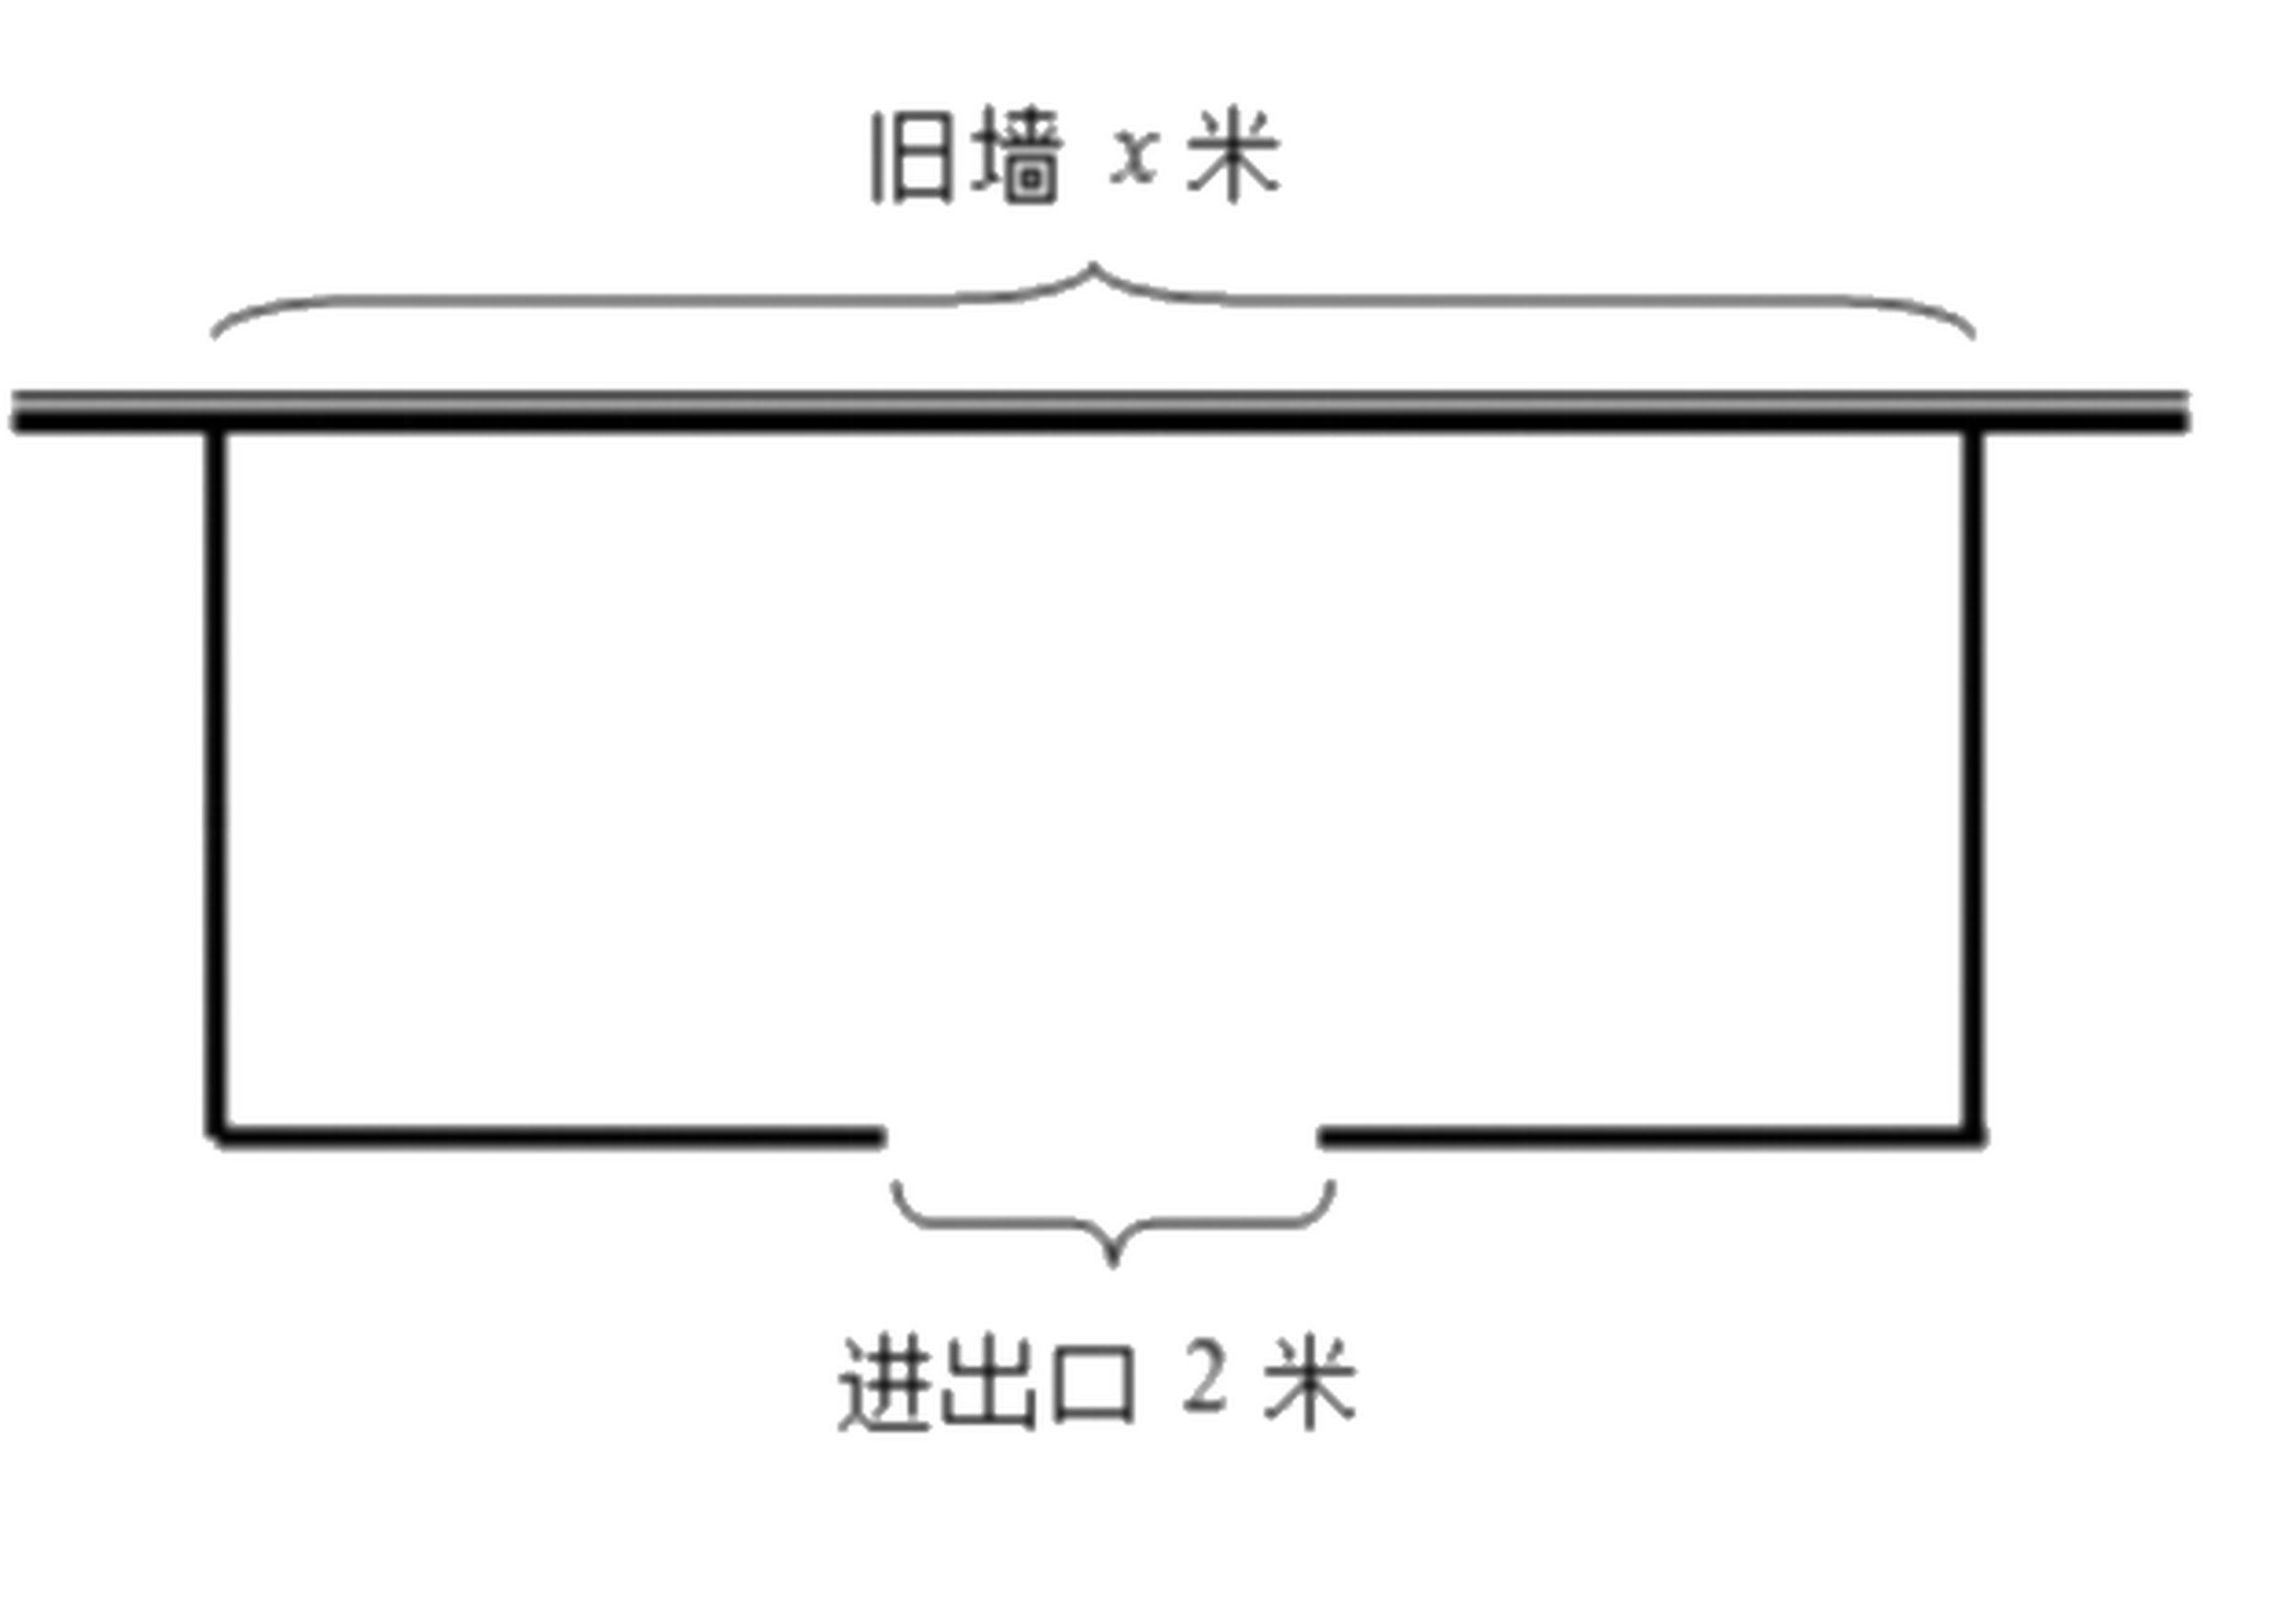
\includegraphics[width=0.60\textwidth]{figures/gao144_q17.png}
\end{center}

(1) 写出总费用 $y$ 关于 $x$ 的表达式;

(2) 试确定 $x$，使修建此矩形场地围墙的总费用最小，并求出最小总费用.

\ifanswer
\solbegin
\step{(1) 设矩形的另一边长为 $a$ 米，}
\step{则 $y=45x+180(x-2)+180\times2a=225x+360a-360$，}
\step{由已知 $xa=360$，得 $a=\dfrac{360}{x}$，所以 $y=225x+\dfrac{360^2}{x}-360(x>0)$;}
\step{(2) 因为 $x>0$，所以 $225x+\dfrac{360^2}{x}\geqslant2\sqrt{225x\cdot\dfrac{360^2}{x}}=10800$，}
\step{所以 $y=225x+\dfrac{360^2}{x}-360\geqslant10440$，}
\step{当且仅当 $225x=\dfrac{360^2}{x}$，即 $x=24$ 时取等号，}
\step{所以当 $x=24$ 米时，修建围墙的总费用最小，最小总费用是 10440 元.}
\solend
\fi

\item 已知集合 $A=\{a_1,a_2,\cdots,a_k\}(k\geqslant2)$，其中 $a_i\in\Z(i=1,2,\cdots,k)$. 定义：若对任意的 $x\in A$，必有 $-x\notin A$，则称集合 $A$ 具有性质 $G$. 由 $A$ 中元素可构成两个点集 $P$ 和 $Q$，$P=\{(x,y)\mid x\in A,y\in A,x+y\in A\}$，$Q=\{(x,y)\mid x\in A,y\in A,x-y\in A\}$，其中 $P$ 有 $m$ 个元素，$Q$ 中有 $n$ 个元素.

(1) 已知集合 $K=\{-1,2,3\}$，判断 $K$ 是否具有性质 $G$; 并写出 $K$ 对应的集合 $P$ 和集合 $Q$;

(2) 若集合 $A=\{1,2,3,4,5,6,7,8,9,10\}$，求对应集合 $Q$ 的元素个数; 一般地，若集合 $A$ 具有性质 $G$，且有 $k$ 个元素，猜测对应的集合 $Q$ 的元素最大个数，并说明理由;

(3) 若集合 $A$ 具有性质 $G$，猜测 $m,n$ 的大小并说明理由.

\ifanswer
\solbegin
\step{(1) 因为 $K=\{-1,2,3\},1,-2,-3$ 都不属于集合 $K$，}
\step{所以集合 $K$ 具有性质 $G$，}
\step{对应集合 $P=\{(-1,3),(3,-1)\},Q=\{(2,-1),(2,3)\}$;}
\step{(2) $A=\{1,2,3,4,5,6,7,8,9,10\}$，则对应集合 $Q$ 中的元素为:}
\step{$(2,1),(3,2),\cdots,(9,8),(10,9)$,}
\step{$(3,1),(4,2),\cdots,(9,7),(10,8)$,}
\step{$(4,1),(5,2),\cdots,(9,6),(10,7)$,}
\step{$\cdots$}
\step{$(9,1),(10,2)$,}
\step{$(10,1)$,}
\step{共有 $9+8+7+\cdots+2+1=45$ 个元素，即对应集合 $Q$ 的元素个数 45;}
\step{集合 $A$ 有 $k$ 个元素，猜测对应的集合 $Q$ 的最大个数为 $\dfrac{k^2-k}{2}$. 理由如下:}
\step{由题意得集合 $A$ 的元素构成有序数对 $(a_i,a_j)(i,j\in\N^*,i\leqslant k,j\leqslant k)$，}
\step{共有 $k^2$ 个，因为 $0\notin A$，所以 $(a_i,a_i)\notin Q$，}
\step{又因为 $a\in A$ 时，$-a\notin A$，所以 $(a_i,a_j)\in Q$ 时，$(a_j,a_i)\notin Q$，}
\step{所以集合 $Q$ 的元素个数为 $\dfrac{k^2-k}{2}$ 个，}
\step{(3) 当集合 $A$ 具有性质 $G$ 时，}
\step{①对于 $(a,b)\in P$，由定义得 $a\in A,b\in A,a+b\in A$，}
\step{又因为集合 $A$ 具有性质 $G$，所以 $(a+b,a)\in Q$，}
\step{如果 $(a,b),(c,d)$ 是 $P$ 中的不同元素，}
\step{那么 $a=c,b=d$ 中至少有一个不成立，}
\step{于是 $b=d,a+b=c+d$ 中至少有一个不成立，}
\step{故 $(a+b,b)$ 和 $(c+d,d)$ 也是 $Q$ 中不同的元素，}
\step{可见 $P$ 的元素个数不多于 $Q$ 的元素个数，即 $m\leqslant n$;}
\step{②对于 $(a,b)\in Q$，由定义得 $a\in A,b\in A,a-b\in A$，}
\step{又因为集合 $A$ 具有性质 $G$，则 $(a-b,b)\in P$，}
\step{如果 $(a,b),(c,d)$ 是 $Q$ 中的不同元素，}
\step{那么 $a=c,b=d$ 中至少有一个不成立，}
\step{于是 $b=d,a-b=c-d$ 中至少有一个不成立，}
\step{故 $(a-b,b)$ 和 $(c-d,d)$ 也是 $P$ 中不同的元素，}
\step{可见 $Q$ 的元素个数不多于 $P$ 的元素个数，即 $n\leqslant m$，}
\step{由①②得 $m=n$.}
\solend
\fi

\end{enumerate}

\end{document}
"
% 紧凑版：xelatex "\def\iscompact{1}% 高一144_风华中学_期中.tex
%   —— 高一上数学"2026-2027 年风华中学高一上期中"（试卷版/答案版/紧凑版）
% 试卷版：xelatex 高一144_风华中学_期中.tex
% 答案版：xelatex "\def\isanswer{1}% 高一144_风华中学_期中.tex
%   —— 高一上数学"2026-2027 年风华中学高一上期中"（试卷版/答案版/紧凑版）
% 试卷版：xelatex 高一144_风华中学_期中.tex
% 答案版：xelatex "\def\isanswer{1}\input{高一144_风华中学_期中.tex}"
% 紧凑版：xelatex "\def\iscompact{1}\input{高一144_风华中学_期中.tex}"
%
% ① 原始材料：微信公众号"魔都数学加油站"文章，连载"27学年高一144"，原文标题
% "27学年高一144——2026-2027年上海市风华中学高一上期中"；
% 原文链接：https://mp.weixin.qq.com/s/ylUlbXfudWOYC-jlH3jyjw 。
% 正文为 10 张 PNG 页，题目下印【解析】，为讲评版。
% 各页分辨率：01/02/03/05/06/07/09/10 为 2560×3620，04/08 为 4762×6735。
% 题目、解析均据原图转录；卷面粉红色水印"魔都数学加油站"及公众号页脚未录入。
% 全卷插图情况：Q17 有一幅矩形场地示意图（旧墙 x 米 / 进出口 2 米），从 07 页裁出、
%   去粉色水印去色 4× LANCZOS 放大存 figures/gao144_q17.png；其余 9 页逐页通读
%   确认无题目配图、无表格、亦无"题干写如图而源码漏图"一处。
%
% 卷首标题：原卷印作"2026-2027 年风华中学高一上期中"，年份区间按全稿惯例排 en dash；
% 原卷卷面未印副标题，本稿按同期中卷（高一140／141／143）知识模块口径补出
% "集合与常用逻辑用语、不等式、函数"：集合与逻辑见 Q3、Q7、Q9、Q10、Q12、Q16、Q18，
% 不等式见 Q6、Q11、Q13、Q14、Q15、Q17，函数见 Q4、Q5、Q8、Q9。
%
% 题号体例：本卷共 16 题——一、填空题 3—10（8 题）、二、选择题 11—13（3 题）、
% 三、解答题 14—18（5 题）。三节分别 \setcounter{enumi}{2}／{10}／{13}。
% 原卷从第 3 题起、无第 1、2 题，本稿保留原题号；全卷无附加题节。
%
% ② 与原卷的排版差异：
%   ① 原文从第 3 题起，本稿保留原题号；共 16 题三节；
%   ② 原卷 15 题题下印【解析】，唯 Q11 未印【解析】、只把答案"（ BD ）"直接印在
%      题干括号内（放大 04 页 A/B 选项与 05 页 C/D 选项衔接处确认，见 ⑤）；
%      按 高一128／94／106／140 成例：Q11 试卷版括号留空 \mbox{（\quad）}、
%      答案版另提 \ans{$BD$}、不补造原卷没有的解析；其余 15 题印【解析】、
%      括号内一律留空、不另提 \ans{}（Q12 选 C、Q13 选 B 在解析末句"故选 …"）；
%      答案版【答案】/【解析】标记数 = 16（1 个 \ans + 15 个 \solbegin）= 全卷题数；
%      正文 Q11 对应处另有 % 注；
%   ③ 原卷卷面未印副标题，本稿按知识模块口径补出；
%   ④ 原卷填空横线按全稿惯例排 \blankline[4.4em]；选择题括号排 \mbox{（\quad）}，
%      选项段前按惯例加 \keepwithprev；解答题不留作答区、不加 \anspace
%      （原卷为讲评版，与 129／131／132／133／136／140／141／143 同）；
%   ⑤ 数集：Q9 题干与解析"a,b∈R"、Q12 题干"U=R"、Q15 题干"x,y∈R"原卷印
%      斜体或黑板粗体 R，Q18 题干"a_i∈Z"印黑板粗体 Z、Q18 解析"i,j∈N*"印
%      黑板粗体 N，按全稿惯例统一改 \R／\Z／\N^*；绝对值排 \lvert…\rvert，
%      集合描述竖线排 \mid；不等号按全稿惯例排 \leqslant／\geqslant；
%      补集照原卷上划线排 \overline{A}／\overline{B}；空集记号 \varnothing；
%   ⑥ 子题标号 (1)(2)(3) 原卷印半角括号，照录；圈数字 ①② 在正文（文本模式）
%      按原卷照录（Q15、Q18 解析），未进数学式；数学式内半角逗号照录
%      （Q12 解析"$A=(1,2),B=(0,6)$"、Q18 解析"$(a_i,a_j)(i,j\in\N^*,i\leqslant k,j\leqslant k)$"、
%      Q15 解析"$x=1,y=-1$"、Q18 解析"$a=c,b=d$"等，为全稿惯例、非笔误）；
%      全卷行末西文句点照录为 ASCII `.`；行中全角逗号／顿号照录；
%      Q18 解析集合描述中的"或"用 \text{ 或 } 置于数学式内；
%   ⑦ 题干中的中文弯引号按原卷照录（Q3 的" x∈A "／" x∈B "与 Q15 (2) 的命题
%      引号，含引号内空格），注释内一律 ASCII 引号；
%   ⑧ Q17 配图：题干写"如图所示"，配图居中排在题干之后、子问之前，三版都出；
%      在 Q17 \item 之前加 \needvspace{10cm} 把"题干＋图"整块推走。Q17 是
%      "三、解答题"节内第 4 题（非节首题），故守卫放在 \item 之前而非 \bigsec
%      之前不会让节标题孤落页末（B 类）；三版切页审计均"合计异常：无"；
%   ⑨ 跨页续印按题合并：Q3 在 01 页；Q4/5/6 在 01 页（Q6 解析续到 02 页顶）；
%      Q7/8/9 在 02 页（Q9 题干跨 02→03）；Q10 在 03 页、解析跨 03→04（很长，
%      按余数分组 A₁/A₂/A₃）；Q11 在 04 页（"二、选择题"节标题也在 04 页下部）、
%      Q12/13 在 05 页（"三、解答题"标题在 05 页下部）；Q14 在 05 页末、解析在 06 页；
%      Q15/16 在 06 页（Q16 续到 07 页）；Q17 在 07 页；Q18 在 08 页、解析跨
%      08/09/10 页（性质 G 压轴，3 问，很长）；本稿按题连排，不丢行、不并折行；
%   ⑩ Q8 解析"法一：""法二："两处标签经放大 02 页逐字确认原卷均印红色
%      （见 ⑤）；按全稿惯例（高一53 成例）不引入红色、均照录为黑体着色
%      \stepm{法一：}{…}／\stepm{法二：}{…}，不改 common.sty；
%      文件头在此注明原卷为红色；
%   ⑪ "图像／图象"逐处核：全卷未出现"图像"或"图象"字样，无统一问题；
%   ⑫ \left…\right 不得拆到不同 $…$ 组；cases 块整体算一个印刷行；
%      Q4 分式与 8×(-3/4) 同一 $…$ 组，Q13 的 \left(\frac1x+\frac2y\right) 同理。
%
% ③ 行数复核：一条 \step／\stepm 行 = 原卷解析的一个印刷行，cases 块作一个印刷行计。
%   逐题数（含 \stepm）：Q3：3；Q4：1；Q5：1；Q6：5；Q7：4；Q8：8（6 \step
%   ＋ 2 \stepm，法一/法二标签各占 1 行）；Q9：6；Q10：23；Q11：0（原卷无解析，
%   答案另提 \ans{$BD$}）；Q12：5；Q13：3；Q14：5；Q15：8；Q16：7；Q17：7；
%   Q18：32。合计 116 条 \step ＋ 2 条 \stepm ＝ 118 个印刷行，与原卷逐题相等。
%   全卷 15 题设 \solbegin…\solend ＋ Q11 一处 \ans{}，答案版【答案】/【解析】
%   标记数 = 16 = 全卷题数。
%
% ④ 判别式／子集符号结论（逐处放大原图照录、不得统一）：
%   判别式全卷 2 处，逐页放大扫过 10 页确认（Q4 为分式指数化简、不含判别式）：
%     · Q9【解析】"所以 △=a^2-4b=0" 原卷印细线、扁等边三角（宽≈高、笔画细，
%       放大见 /tmp/gao144fh/z_q9_tri.png、z_tri_Q9.png），照录 \triangle；
%     · Q15 (2)【解析】cases 块"Δ=(a-2)^2-4(a-2)≤0" 原卷印等腰偏高、粗笔画
%       三角（高>宽，放大见 z_q15_tri.png、z_tri_Q15.png），照录 \Delta；
%   两形不同、全卷混用，逐处照录不统一（参照 高一142 头注④口径）。
%   子集符号全卷 4 处，逐处放大核：
%     · Q3 解析"所以 B⊆A"、Q16 (1) 解析"所以 B⊆A" 原卷均印带下划线的 ⊆
%       （z_q3_symbol.png、z_q16_subset2.png），照录 \subseteq；
%     · Q12 选项 B"$\overline{A}\subset B$" 原卷印单线 ⊂（z_q12_opts2.png），
%       照录 \subset；Q12 解析"$\overline{A}=(-\infty,1]\cup[2,+\infty)\not\subset B$"
%       原卷印单线带斜杠 ⊄（z_q12_notsym3.png），照录 \not\subset；
%   \subset 与 \subseteq 混用，逐处照录不统一。补集照原卷上划线 \overline{A}／
%   \overline{B}，空集 \varnothing，数集 \R／\Z／\N^* 归一见 ② ⑤。
%
% ⑤ 存疑／特殊体例（主会话逐处放大原图复核确认，照录未改，正文对应处另有 % 注）：
%   1. 第 11 题原卷把答案"（ BD ）"直接印在题干括号内、题下未印【解析】
%      （放大 04 页 A/B 选项与 05 页 C/D 选项衔接处确认：05 页顶 C/D 选项后
%      直接接第 12 题）。按 高一128／94／106／140 成例括号留空、另提
%      \ans{$BD$}，不补造解析（不编造）。
%   2. 第 10 题题干"集合 $S$ 为集合 $M=\{1,2,3,4,\cdots,2026\}$，的子集"在
%      集括号与"的子集"之间原卷多印一个全角逗号（放大 03 页确认），
%      按存疑照录未删，正文对应处另有 % 注。
%   3. 第 8 题解析"法一：""法二："两处原卷均印红色（放大 02 页逐字确认），
%      按全稿惯例不引入红色、两处均照录为黑体着色 \stepm（见 ② ⑩）。
%   全卷除此 3 条外未发现其它笔误／自相矛盾处。
%
% ⑥ 跨页续印按题合并说明：见 ② ⑨。
%
\documentclass[a4paper,11pt]{article}
\usepackage{common}

\begin{document}

\examtitlest[3]{2026--2027 年风华中学高一上期中}{集合与常用逻辑用语、不等式、函数}

\bigsec{一、填空题}

\begin{enumerate}
\setcounter{enumi}{2}

\item $A=\{x\mid x>4\}$，$B=\{x\mid x>a\}$，若命题 “ $x\in A$ ” 是命题 “ $x\in B$ ” 的必要条件，则 $a$ 的取值范围是\blankline[4.4em].

\ifanswer
\solbegin
\step{因为 “ $x\in A$ ” 是命题 “ $x\in B$ ” 的必要条件，所以 $B\subseteq A$，}% 子集符号原卷印带下划线 $\subseteq$，照录
\step{因为 $A=\{x\mid x>4\}$，$B=\{x\mid x>a\}$，所以 $a\geqslant4$，}
\step{所以 $a$ 的取值范围是 $\{a\mid a\geqslant4\}$.}
\solend
\fi

\item 已知 $a>0,b>0$，化简式子：$\dfrac{8a^{\frac34}b^3}{\left(a^{\frac16}b^{\frac32}\right)\left(-\dfrac43 a^{\frac1{12}}b^{\frac12}\right)}=$\blankline[4.4em].

\ifanswer
\solbegin
\step{$\dfrac{8a^{\frac34}b^3}{\left(a^{\frac16}b^{\frac32}\right)\left(-\dfrac43 a^{\frac1{12}}b^{\frac12}\right)}=8\times\left(-\dfrac34\right)a^{\frac34-\frac16-\frac1{12}}b^{3-\frac32-\frac12}=-6a^{\frac12}b=-6b\sqrt a$.}
\solend
\fi

\item 已知 $\lg2=a$，$\lg3=b$，则 $\log_5 6=$\blankline[4.4em]（结果用 $a,b$ 表示）.

\ifanswer
\solbegin
\step{$\log_5 6=\dfrac{\lg6}{\lg5}=\dfrac{\lg2+\lg3}{1-\lg2}=\dfrac{a+b}{1-a}$.}
\solend
\fi

\item 若关于 $x$ 的不等式 $ax>b$ 的解集为 $(-\infty,2)$，则不等式 $bx+a>0$ 的解集为\blankline[4.4em].

\ifanswer
\solbegin
\step{因为不等式 $ax>b$ 的解集为 $(-\infty,2)$，所以 $a<0$，}
\step{所以由不等式解得 $x<\dfrac ba$，所以 $\dfrac ba=2$，即 $b=2a$，}
\step{代入不等式 $bx+a>0$，得 $2ax+a>0$，}
\step{因为 $a<0$，所以不等式化为 $2x+1<0$，解得 $x<-\dfrac12$，}
\step{故不等式的解集为 $\left(-\infty,-\dfrac12\right)$.}
\solend
\fi

\item 如果集合 $A=\{x\mid x^2-4x\leqslant0\}$，$B=\{x\mid x^2+ax+b\leqslant0\}$，$A\cap B=\{x\mid3\leqslant x\leqslant4\}$，$A\cup B=\{x\mid0\leqslant x\leqslant5\}$，则 $a+b=$\blankline[4.4em].

\ifanswer
\solbegin
\step{由题意得 $A=\{x\mid x^2-4x\leqslant0\}=[0,4]$，}
\step{又因为 $A\cap B=\{x\mid3\leqslant x\leqslant4\}$，$A\cup B=\{x\mid0\leqslant x\leqslant5\}$，}
\step{所以 $B=\{x\mid3\leqslant x\leqslant5\}$，即方程 $x^2+ax+b=0$ 的两根为 $3,5$，}
\step{由韦达定理得 $\begin{cases}3+5=-a\\3\times5=b\end{cases}$，解得 $a=-8$，$b=15$，所以 $a+b=15-8=7$.}
\solend
\fi

% 第 8 题：原卷"法一：""法二："两处标签均印红色（8× 放大确认）；按交办口径
% "法一"用普通 \step、"法二："排 \stepm（加粗着色、不引红色），见头注 ② ⑩／⑤
\item 若关于 $x$ 的方程 $\lvert x-1\rvert+\lvert\pi-x\rvert=\pi-1$ 的解集为\blankline[4.4em].

\ifanswer
\solbegin
\stepm{法一：}{因为 $\lvert x-1\rvert+\lvert\pi-x\rvert=\begin{cases}x-1+x-\pi,x\geqslant\pi\\\pi-1,1<x<\pi\\1-x+\pi-x,x\leqslant1\end{cases}=\begin{cases}2x-1-\pi,x\geqslant\pi\\\pi-1,1<x<\pi\\1+\pi-2x,x\leqslant1\end{cases}$.}
\step{当 $x\geqslant\pi$ 时，令 $2x-1-\pi=\pi-1$，得 $x=\pi$；}
\step{当 $1<x<\pi$ 时，$\lvert x-1\rvert+\lvert\pi-x\rvert=\pi-1$ 恒成立；}
\step{当 $x\leqslant1$ 时，令 $1+\pi-2x=\pi-1$，得 $x=1$.}
\step{综上所述，方程 $\lvert x-1\rvert+\lvert\pi-x\rvert=\pi-1$ 的解集为 $[1,\pi]$.}
\stepm{法二：}{因为 $\lvert x-1\rvert+\lvert\pi-x\rvert\geqslant\lvert x-1+\pi-x\rvert=\pi-1$，}
\step{当且仅当 $(x-1)(\pi-x)\geqslant0$ 时取等号，}
\step{故方程 $\lvert x-1\rvert+\lvert\pi-x\rvert=\pi-1$ 的解集为 $[1,\pi]$.}
\solend
\fi

% 第 9 题：题干跨 02→03 页；解析判别式原卷印细线扁等边三角 $\triangle$，照录
\item 已知函数 $f(x)=x^2+ax+b(a,b\in\R)$ 和 $x$ 轴有且只有一个交点，若关于 $x$ 的不等式 $f(x)<c$ 的解集为 $(m,m+6)$，则 $c=$\blankline[4.4em].

\ifanswer
\solbegin
\step{因为函数 $f(x)=x^2+ax+b(a,b\in\R)$ 和 $x$ 轴有且只有一个交点，}
\step{所以 $\triangle=a^2-4b=0$，即 $b=\dfrac{a^2}{4}$，}% 判别式原卷印扁等边三角 $\triangle$，照录
\step{不等式 $f(x)<c$ 的解集为 $(m,m+6)$，}
\step{即 $x^2+ax+\dfrac{a^2}{4}-c<0$ 的解集为 $(m,m+6)$，}
\step{所以方程 $x^2+ax+\dfrac{a^2}{4}-c=0$ 的两个根为 $x_1=m$，$x_2=m+6$，}
\step{所以 $\begin{cases}x_1+x_2=2m+6=-a\\x_1x_2=m(m+6)=\dfrac{a^2}{4}-c\end{cases}$，消去 $m$ 得 $\dfrac{a^2}{4}-9=\dfrac{a^2}{4}-c$，解得 $c=9$.}
\solend
\fi

% 第 10 题：原卷题干在集括号与"的子集"之间多印一个全角逗号，照录未改（存疑，见头注 ⑤）
\item 已知集合 $S$ 为集合 $M=\{1,2,3,4,\cdots,2026\}$，的子集，并且集合 $S$ 中任意两个元素之和不能被 3 整除，则集合 $S$ 中元素个数的最大值为\blankline[4.4em].

\ifanswer
\solbegin
\step{对于集合 $M=\{1,2,3,4,\cdots,2026\}$，}
\step{所有被 3 除余数为 0 的元素组成的集合为 $A_3=\{3,6,9,\cdots,2025\}$，}
\step{元素个数为 675;}
\step{所有被 3 除余数为 1 的元素组成的集合为 $A_1=\{1,4,7,\cdots,2026\}$，}
\step{元素个数为 676;}
\step{所有被 3 除余数为 2 的元素组成的集合为 $A_2=\{2,5,8,\cdots,2024\}$，}
\step{元素个数为 675;}
\step{集合 $S$ 中任意两个元素之和不能被 3 整除，}
\step{若两个元素分别来自 $A_1$ 和 $A_2$，则两数之和除以 3 的余数为 $1+2=3\equiv0$，}
\step{即和能被 3 整除，}
\step{所以 $S$ 不能同时包含 $A_1$ 和 $A_2$ 中的元素，}
\step{即 $S$ 最多只能选取 $A_1$、$A_2$ 一个集合中的全部元素;}
\step{若两个元素都来自 $A_3$，则两数之和除以 3 的余数为 $0+0=0$，即和能被 3 整除，}
\step{所以 $S$ 中最多包含 $A_3$ 中的 1 个元素;}
\step{对 $A_1$ 内的任意两个元素，其和除以 3 的余数为 $1+1=2$，不能被 3 整除;}
\step{$A_1$ 中元素与 $A_3$ 中元素的和除以 3 余数为 $1+0=1$，不能被 3 整除，}
\step{所以 $A_1$ 的全部元素与 $A_3$ 中的任意 1 个元素的组合满足题意;}
\step{对 $A_2$ 内的任意两个元素，其和除以 3 的余数为 $2+2=4\equiv1$，不能被 3 整除;}
\step{$A_2$ 中元素与 $A_3$ 中元素的和除以 3 的余数为 $2+0=2$，不能被 3 整除，}
\step{所以 $A_2$ 的全部元素与 $A_3$ 中任意 1 个元素的组合也满足题意.}
\step{故若选取 $A_2$ 全部元素加 1 个 $A_3$ 元素，总个数为 $675+1=676$;}
\step{选取 $A_1$ 全部元素加 1 个 $A_3$ 元素，总个数为 $676+1=677$;}
\step{所以集合 $S$ 中元素个数的最大值为 677.}
\solend
\fi

\end{enumerate}

\bigsec{二、选择题}

\begin{enumerate}
\setcounter{enumi}{10}

% 第 11 题：原卷把答案"（ BD ）"直接印在题干括号内、题下无【解析】（放大 04 页 A/B 选项
% 与 05 页 C/D 选项衔接处确认）。按 高一128／94／106／140 成例：试卷版括号留空、
% 答案版另提 \ans{$BD$}、不补造原卷没有的解析（不编造）。
\item 已知实数 $a,b$，下列四个不等式中正确的是\mbox{（\quad）}

\keepwithprev
A. $a+\dfrac1a\geqslant2$\qquad B. $\sqrt{a^2+2}+\dfrac{1}{\sqrt{a^2+2}}\geqslant2$

C. $\dfrac{a+b}{2}\leqslant\sqrt{ab}$\qquad D. $a^2+b^2\geqslant2ab$

\ifanswer
\ans{$BD$}
\fi

\item 若全集 $U=\R$，$A=\{x\mid x^2-3x+2<0\}$，$B=\{x\mid0<x<6\}$，则\mbox{（\quad）}

\keepwithprev
A. $A\cap B=B$\qquad B. $\overline{A}\subset B$\qquad C. $A\cap\overline{B}=\varnothing$\qquad D. $A\cup B=A$

\ifanswer
\solbegin
\step{由 $x^2-3x+2<0$，则 $A=(1,2),B=(0,6)$，所以 $A\cap B=(1,2)=A,A$ 错误;}
\step{$\overline{A}=(-\infty,1]\cup[2,+\infty)\not\subset B$，$B$ 错误;}
\step{$\overline{B}=(-\infty,0]\cup[6,+\infty)$，所以 $A\cap\overline{B}=\varnothing,C$ 正确;}
\step{$A\cup B=(0,6)\ne A,D$ 错误.}
\step{故选 $C$.}
\solend
\fi

\item 已知正数 $x$、$y$ 满足 $\dfrac1x+\dfrac2y=1$，不等式 $3x+2y-1>m$ 恒成立，则实数 $m$ 的取值范围是\mbox{（\quad）}

\keepwithprev
A. $(-\infty,4+6\sqrt2)$\qquad B. $(-\infty,6+4\sqrt3)$\qquad C. $(6+4\sqrt2,+\infty)$\qquad D. $(8+4\sqrt3,+\infty)$

\ifanswer
\solbegin
\step{$3x+2y=(3x+2y)\left(\dfrac1x+\dfrac2y\right)=7+\dfrac{6x}{y}+\dfrac{2y}{x}\geqslant7+2\sqrt{\dfrac{6x}{y}\cdot\dfrac{2y}{x}}=7+4\sqrt3$，}
\step{当且仅当 $\dfrac{6x}{y}=\dfrac{2y}{x}$，即 $y=\sqrt3x=\sqrt3+2$ 时取等号，}
\step{故要使原式成立，只需 $m<6+4\sqrt3$. 故选 $B$.}
\solend
\fi

\end{enumerate}

\bigsec{三、解答题}

\begin{enumerate}
\setcounter{enumi}{13}

\item 解关于 $x$ 的不等式：

(1) $x^2-2\lvert x\rvert-3>0$；

(2) $\dfrac{2x-1}{x+2}<1$.

\ifanswer
\solbegin
\step{(1) 原不等式等价于 $(\lvert x\rvert-3)(\lvert x\rvert+1)>0$，}
\step{$\lvert x\rvert+1>0$，故 $\lvert x\rvert>3$，解得 $x<-3$ 或 $x>3$，}
\step{故不等式的解集为 $(-\infty,-3)\cup(3,+\infty)$.}
\step{(2) 已知 $\dfrac{2x-1}{x+2}<1$，则 $\dfrac{2x-1}{x+2}-1<0$，即 $\dfrac{x-3}{x+2}<0$，}
\step{等价于 $(x-3)(x+2)<0$，解得 $-2<x<3$，故不等式的解集为 $(-2,3)$.}
\solend
\fi

\item (1) 已知 $x,y\in\R$，比较 $x^2+y^2$ 与 $2x-2y-2$ 的大小.

(2) “不等式 $(a-2)x^2+(a-2)x+1\geqslant0$ 对一切实数恒成立” 是假命题，求实数 $a$ 的取值范围.

\ifanswer
\solbegin
\step{(1) $x^2+y^2-(2x-2y-2)=x^2+y^2-2x+2y+2=(x-1)^2+(y+1)^2\geqslant0$，}
\step{故 $x^2+y^2\geqslant2x-2y-2$，当且仅当 $x=1,y=-1$ 时取等号.}
\step{(2) 先求命题 “$(a-2)x^2+(a-2)x+1\geqslant0$ 对一切实数恒成立” 为真，}
\step{①当 $a-2=0$ 时，即 $a=2$，不等式化为 $1\geqslant0$，成立，符合条件，}
\step{②当 $a-2\ne0$ 时，则 $\begin{cases}a-2>0\\\Delta=(a-2)^2-4(a-2)\leqslant0\end{cases}$，解得 $2<a\leqslant6$，}% 判别式原卷印等腰偏高三角 $\Delta$，照录
\step{综上①②，命题为真时 $2\leqslant a\leqslant6$，}
\step{该命题为假命题，则 $a<2$ 或 $a>6$，}
\step{所以实数 $a$ 的取值范围是 $(-\infty,2)\cup(6,+\infty)$.}
\solend
\fi

\item 设集合 $A=\{x\mid-1\leqslant x\leqslant2\}$，$B=\{x\mid m-1<x<2m+1\}$.

(1) 若 $A\cup B=A$，求实数 $m$ 的取值范围;

(2) 若 $B\cap\overline{A}$ 中只有一个整数 $-2$，求实数 $m$ 的取值范围.

\ifanswer
\solbegin
\step{(1) 因为 $A\cup B=A$，所以 $B\subseteq A$，}% 子集符号原卷印带下划线 $\subseteq$，照录
\step{当 $B=\varnothing$ 时，有 $m-1\geqslant2m+1$，解得 $m\leqslant-2$；}
\step{当 $B\ne\varnothing$ 时，有 $\begin{cases}m-1<2m+1\\m-1\geqslant-1\\2m+1\leqslant2\end{cases}$，解得 $0\leqslant m\leqslant\dfrac12$，}
\step{所以实数 $m$ 的取值范围是 $(-\infty,-2]\cup\left[0,\dfrac12\right]$;}
\step{(2) 由集合 $A=\{x\mid-1\leqslant x\leqslant2\}$，得 $\overline{A}=\{x\mid x<-1\text{ 或 }x>2\}$，}
\step{若 $B\cap\overline{A}$ 中只有一个整数 $-2$，则 $B\ne\varnothing$，且满足 $\begin{cases}m-1<2m+1\\-3\leqslant m-1<-2\\-2<2m+1\leqslant3\end{cases}$}
\step{解得 $-\dfrac32<m<-1$，所以实数 $m$ 的取值范围是 $\left(-\dfrac32,-1\right)$.}
\solend
\fi

% 第 17 题配图是"题干＋图"整块；守卫放在 \item 之前（Q17 非节首题，不会让节标题孤落页末）
\needvspace{10cm}
\item 现要围建一个面积为 360 平方米的矩形场地，要求矩形场地的一面利用旧墙（利用旧墙需维修），其它三面围墙要新建，在旧墙的对面的新墙上要留一个宽度为 2 米的进出口，如图所示，已知旧墙的维修费用为 45 元/米，新墙的造价为 180 元/米，设利用的旧墙的长度为 $x$ 米，工程总造价为 $y$（单位：元）.

\begin{center}
% 矩形场地示意图取自 07 页右侧，去粉色水印、去色、4× LANCZOS 放大
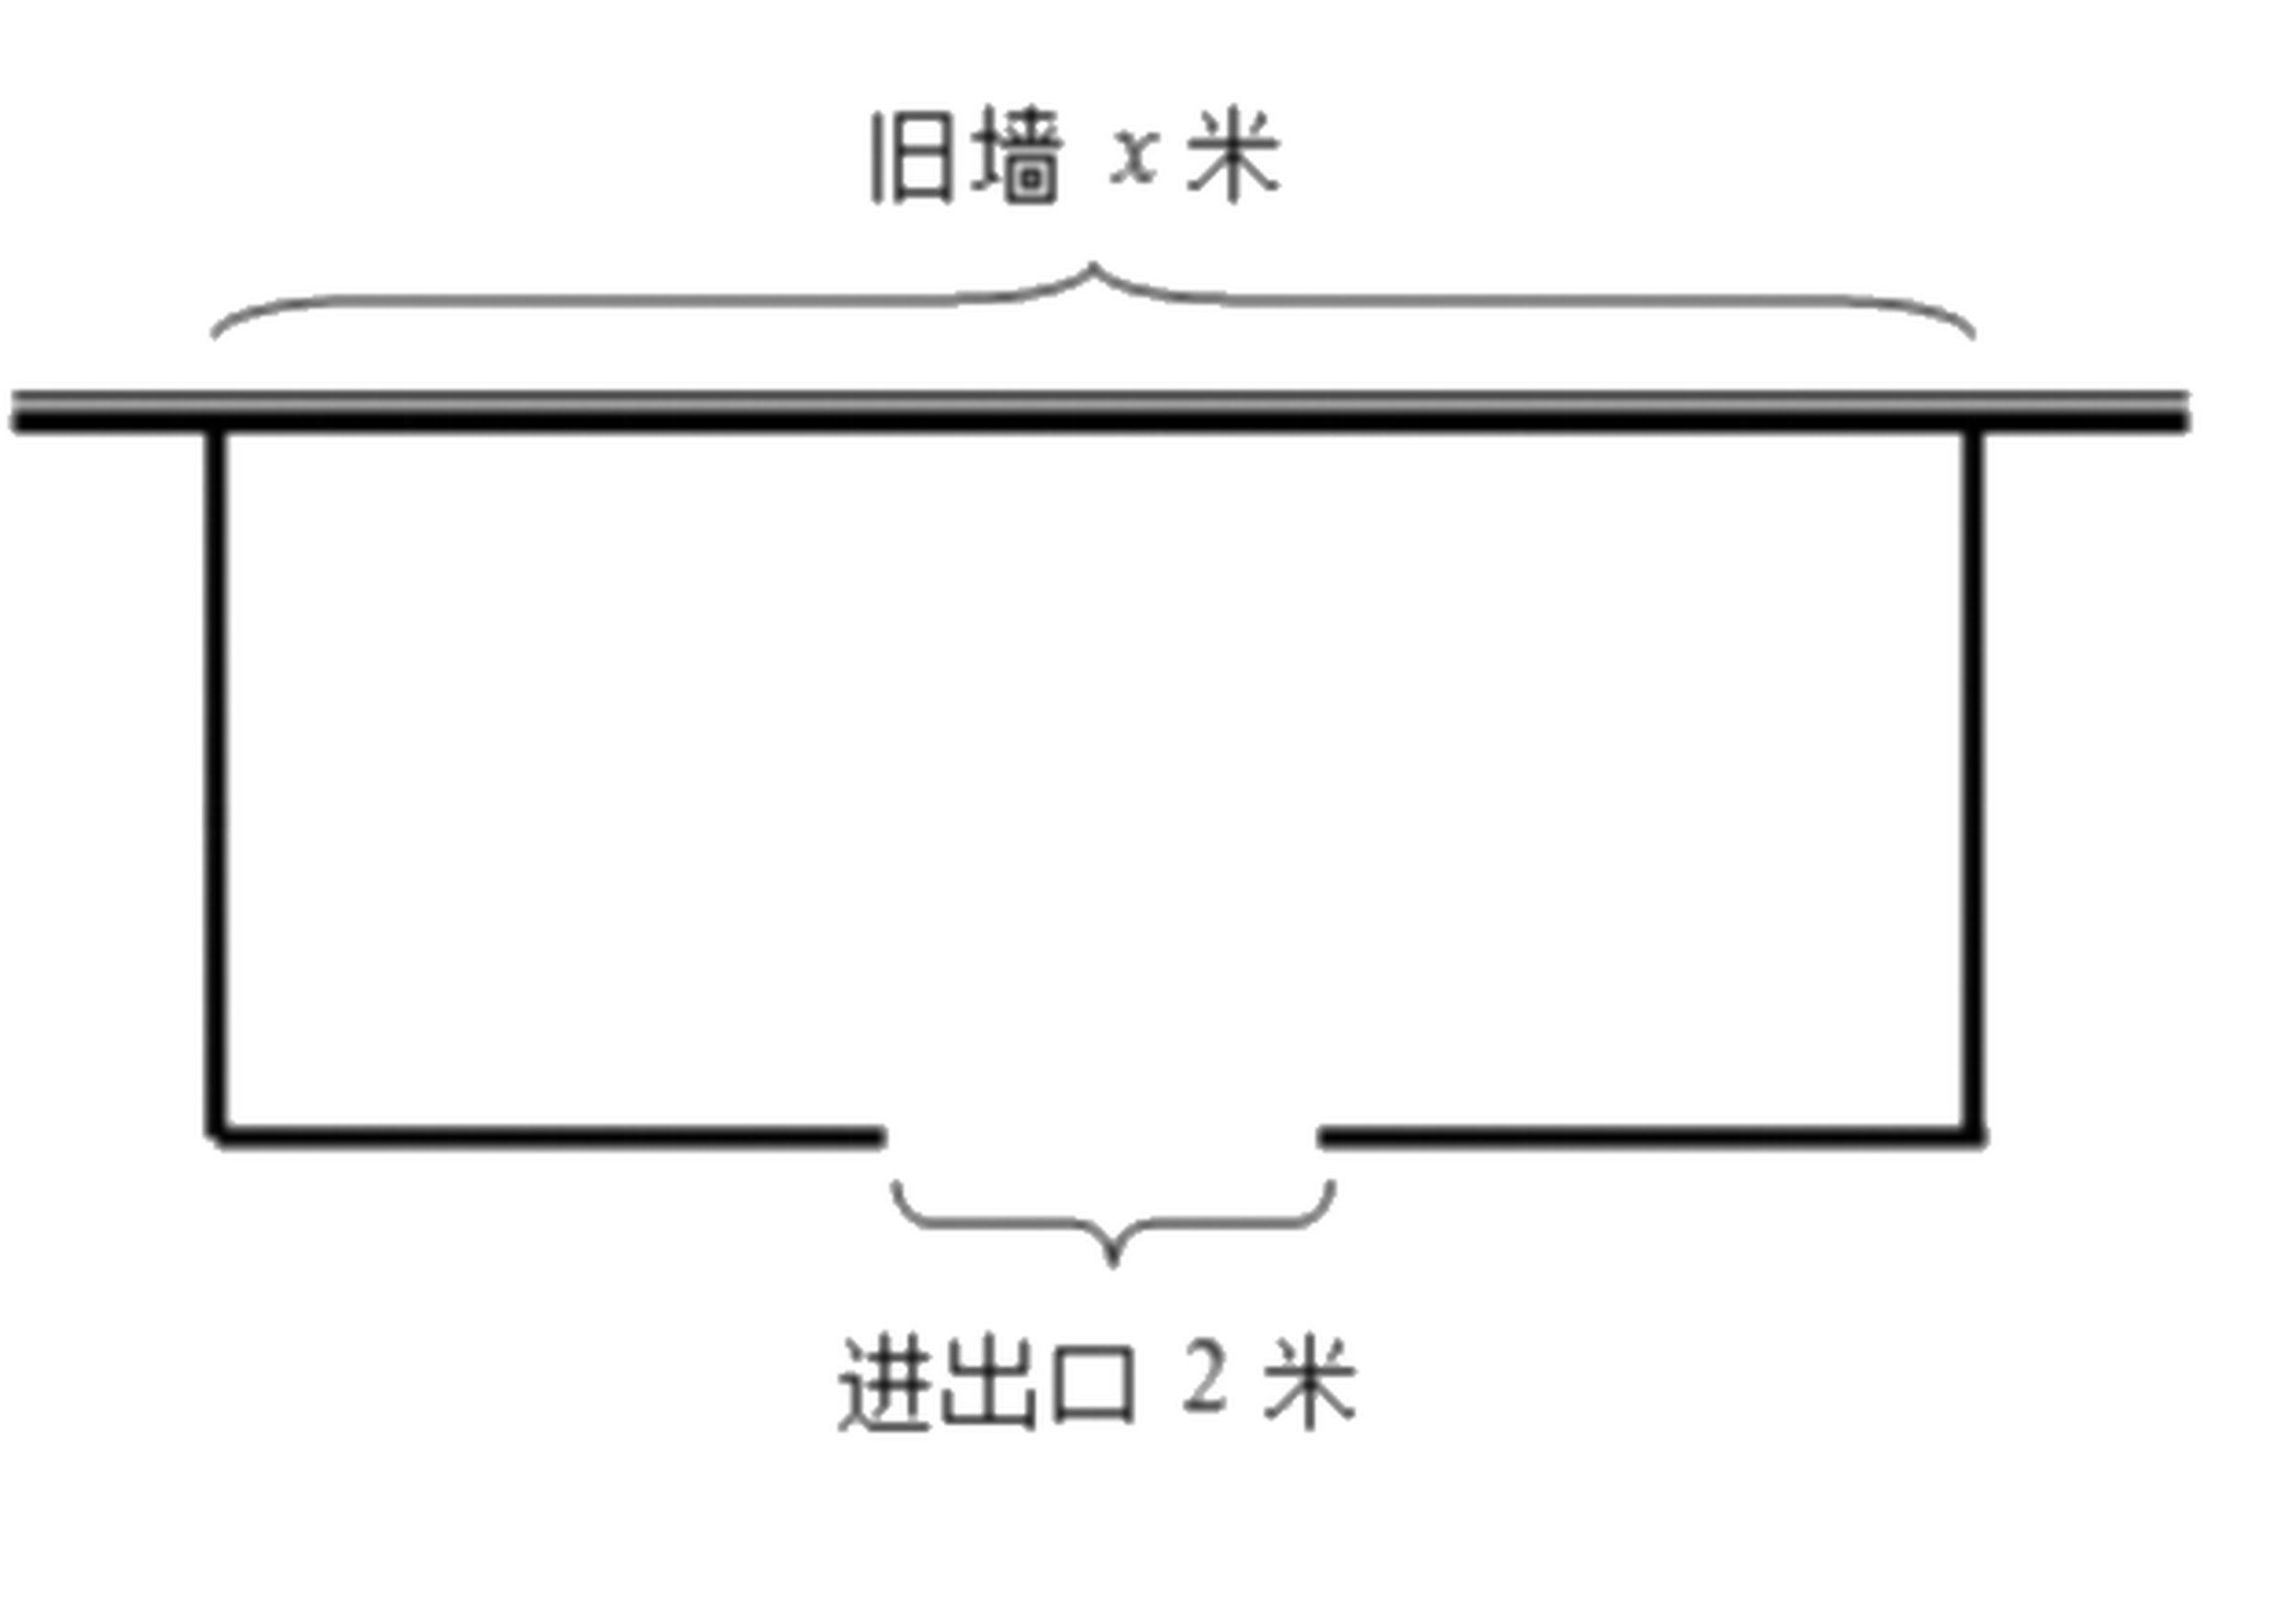
\includegraphics[width=0.60\textwidth]{figures/gao144_q17.png}
\end{center}

(1) 写出总费用 $y$ 关于 $x$ 的表达式;

(2) 试确定 $x$，使修建此矩形场地围墙的总费用最小，并求出最小总费用.

\ifanswer
\solbegin
\step{(1) 设矩形的另一边长为 $a$ 米，}
\step{则 $y=45x+180(x-2)+180\times2a=225x+360a-360$，}
\step{由已知 $xa=360$，得 $a=\dfrac{360}{x}$，所以 $y=225x+\dfrac{360^2}{x}-360(x>0)$;}
\step{(2) 因为 $x>0$，所以 $225x+\dfrac{360^2}{x}\geqslant2\sqrt{225x\cdot\dfrac{360^2}{x}}=10800$，}
\step{所以 $y=225x+\dfrac{360^2}{x}-360\geqslant10440$，}
\step{当且仅当 $225x=\dfrac{360^2}{x}$，即 $x=24$ 时取等号，}
\step{所以当 $x=24$ 米时，修建围墙的总费用最小，最小总费用是 10440 元.}
\solend
\fi

\item 已知集合 $A=\{a_1,a_2,\cdots,a_k\}(k\geqslant2)$，其中 $a_i\in\Z(i=1,2,\cdots,k)$. 定义：若对任意的 $x\in A$，必有 $-x\notin A$，则称集合 $A$ 具有性质 $G$. 由 $A$ 中元素可构成两个点集 $P$ 和 $Q$，$P=\{(x,y)\mid x\in A,y\in A,x+y\in A\}$，$Q=\{(x,y)\mid x\in A,y\in A,x-y\in A\}$，其中 $P$ 有 $m$ 个元素，$Q$ 中有 $n$ 个元素.

(1) 已知集合 $K=\{-1,2,3\}$，判断 $K$ 是否具有性质 $G$; 并写出 $K$ 对应的集合 $P$ 和集合 $Q$;

(2) 若集合 $A=\{1,2,3,4,5,6,7,8,9,10\}$，求对应集合 $Q$ 的元素个数; 一般地，若集合 $A$ 具有性质 $G$，且有 $k$ 个元素，猜测对应的集合 $Q$ 的元素最大个数，并说明理由;

(3) 若集合 $A$ 具有性质 $G$，猜测 $m,n$ 的大小并说明理由.

\ifanswer
\solbegin
\step{(1) 因为 $K=\{-1,2,3\},1,-2,-3$ 都不属于集合 $K$，}
\step{所以集合 $K$ 具有性质 $G$，}
\step{对应集合 $P=\{(-1,3),(3,-1)\},Q=\{(2,-1),(2,3)\}$;}
\step{(2) $A=\{1,2,3,4,5,6,7,8,9,10\}$，则对应集合 $Q$ 中的元素为:}
\step{$(2,1),(3,2),\cdots,(9,8),(10,9)$,}
\step{$(3,1),(4,2),\cdots,(9,7),(10,8)$,}
\step{$(4,1),(5,2),\cdots,(9,6),(10,7)$,}
\step{$\cdots$}
\step{$(9,1),(10,2)$,}
\step{$(10,1)$,}
\step{共有 $9+8+7+\cdots+2+1=45$ 个元素，即对应集合 $Q$ 的元素个数 45;}
\step{集合 $A$ 有 $k$ 个元素，猜测对应的集合 $Q$ 的最大个数为 $\dfrac{k^2-k}{2}$. 理由如下:}
\step{由题意得集合 $A$ 的元素构成有序数对 $(a_i,a_j)(i,j\in\N^*,i\leqslant k,j\leqslant k)$，}
\step{共有 $k^2$ 个，因为 $0\notin A$，所以 $(a_i,a_i)\notin Q$，}
\step{又因为 $a\in A$ 时，$-a\notin A$，所以 $(a_i,a_j)\in Q$ 时，$(a_j,a_i)\notin Q$，}
\step{所以集合 $Q$ 的元素个数为 $\dfrac{k^2-k}{2}$ 个，}
\step{(3) 当集合 $A$ 具有性质 $G$ 时，}
\step{①对于 $(a,b)\in P$，由定义得 $a\in A,b\in A,a+b\in A$，}
\step{又因为集合 $A$ 具有性质 $G$，所以 $(a+b,a)\in Q$，}
\step{如果 $(a,b),(c,d)$ 是 $P$ 中的不同元素，}
\step{那么 $a=c,b=d$ 中至少有一个不成立，}
\step{于是 $b=d,a+b=c+d$ 中至少有一个不成立，}
\step{故 $(a+b,b)$ 和 $(c+d,d)$ 也是 $Q$ 中不同的元素，}
\step{可见 $P$ 的元素个数不多于 $Q$ 的元素个数，即 $m\leqslant n$;}
\step{②对于 $(a,b)\in Q$，由定义得 $a\in A,b\in A,a-b\in A$，}
\step{又因为集合 $A$ 具有性质 $G$，则 $(a-b,b)\in P$，}
\step{如果 $(a,b),(c,d)$ 是 $Q$ 中的不同元素，}
\step{那么 $a=c,b=d$ 中至少有一个不成立，}
\step{于是 $b=d,a-b=c-d$ 中至少有一个不成立，}
\step{故 $(a-b,b)$ 和 $(c-d,d)$ 也是 $P$ 中不同的元素，}
\step{可见 $Q$ 的元素个数不多于 $P$ 的元素个数，即 $n\leqslant m$，}
\step{由①②得 $m=n$.}
\solend
\fi

\end{enumerate}

\end{document}
"
% 紧凑版：xelatex "\def\iscompact{1}% 高一144_风华中学_期中.tex
%   —— 高一上数学"2026-2027 年风华中学高一上期中"（试卷版/答案版/紧凑版）
% 试卷版：xelatex 高一144_风华中学_期中.tex
% 答案版：xelatex "\def\isanswer{1}\input{高一144_风华中学_期中.tex}"
% 紧凑版：xelatex "\def\iscompact{1}\input{高一144_风华中学_期中.tex}"
%
% ① 原始材料：微信公众号"魔都数学加油站"文章，连载"27学年高一144"，原文标题
% "27学年高一144——2026-2027年上海市风华中学高一上期中"；
% 原文链接：https://mp.weixin.qq.com/s/ylUlbXfudWOYC-jlH3jyjw 。
% 正文为 10 张 PNG 页，题目下印【解析】，为讲评版。
% 各页分辨率：01/02/03/05/06/07/09/10 为 2560×3620，04/08 为 4762×6735。
% 题目、解析均据原图转录；卷面粉红色水印"魔都数学加油站"及公众号页脚未录入。
% 全卷插图情况：Q17 有一幅矩形场地示意图（旧墙 x 米 / 进出口 2 米），从 07 页裁出、
%   去粉色水印去色 4× LANCZOS 放大存 figures/gao144_q17.png；其余 9 页逐页通读
%   确认无题目配图、无表格、亦无"题干写如图而源码漏图"一处。
%
% 卷首标题：原卷印作"2026-2027 年风华中学高一上期中"，年份区间按全稿惯例排 en dash；
% 原卷卷面未印副标题，本稿按同期中卷（高一140／141／143）知识模块口径补出
% "集合与常用逻辑用语、不等式、函数"：集合与逻辑见 Q3、Q7、Q9、Q10、Q12、Q16、Q18，
% 不等式见 Q6、Q11、Q13、Q14、Q15、Q17，函数见 Q4、Q5、Q8、Q9。
%
% 题号体例：本卷共 16 题——一、填空题 3—10（8 题）、二、选择题 11—13（3 题）、
% 三、解答题 14—18（5 题）。三节分别 \setcounter{enumi}{2}／{10}／{13}。
% 原卷从第 3 题起、无第 1、2 题，本稿保留原题号；全卷无附加题节。
%
% ② 与原卷的排版差异：
%   ① 原文从第 3 题起，本稿保留原题号；共 16 题三节；
%   ② 原卷 15 题题下印【解析】，唯 Q11 未印【解析】、只把答案"（ BD ）"直接印在
%      题干括号内（放大 04 页 A/B 选项与 05 页 C/D 选项衔接处确认，见 ⑤）；
%      按 高一128／94／106／140 成例：Q11 试卷版括号留空 \mbox{（\quad）}、
%      答案版另提 \ans{$BD$}、不补造原卷没有的解析；其余 15 题印【解析】、
%      括号内一律留空、不另提 \ans{}（Q12 选 C、Q13 选 B 在解析末句"故选 …"）；
%      答案版【答案】/【解析】标记数 = 16（1 个 \ans + 15 个 \solbegin）= 全卷题数；
%      正文 Q11 对应处另有 % 注；
%   ③ 原卷卷面未印副标题，本稿按知识模块口径补出；
%   ④ 原卷填空横线按全稿惯例排 \blankline[4.4em]；选择题括号排 \mbox{（\quad）}，
%      选项段前按惯例加 \keepwithprev；解答题不留作答区、不加 \anspace
%      （原卷为讲评版，与 129／131／132／133／136／140／141／143 同）；
%   ⑤ 数集：Q9 题干与解析"a,b∈R"、Q12 题干"U=R"、Q15 题干"x,y∈R"原卷印
%      斜体或黑板粗体 R，Q18 题干"a_i∈Z"印黑板粗体 Z、Q18 解析"i,j∈N*"印
%      黑板粗体 N，按全稿惯例统一改 \R／\Z／\N^*；绝对值排 \lvert…\rvert，
%      集合描述竖线排 \mid；不等号按全稿惯例排 \leqslant／\geqslant；
%      补集照原卷上划线排 \overline{A}／\overline{B}；空集记号 \varnothing；
%   ⑥ 子题标号 (1)(2)(3) 原卷印半角括号，照录；圈数字 ①② 在正文（文本模式）
%      按原卷照录（Q15、Q18 解析），未进数学式；数学式内半角逗号照录
%      （Q12 解析"$A=(1,2),B=(0,6)$"、Q18 解析"$(a_i,a_j)(i,j\in\N^*,i\leqslant k,j\leqslant k)$"、
%      Q15 解析"$x=1,y=-1$"、Q18 解析"$a=c,b=d$"等，为全稿惯例、非笔误）；
%      全卷行末西文句点照录为 ASCII `.`；行中全角逗号／顿号照录；
%      Q18 解析集合描述中的"或"用 \text{ 或 } 置于数学式内；
%   ⑦ 题干中的中文弯引号按原卷照录（Q3 的" x∈A "／" x∈B "与 Q15 (2) 的命题
%      引号，含引号内空格），注释内一律 ASCII 引号；
%   ⑧ Q17 配图：题干写"如图所示"，配图居中排在题干之后、子问之前，三版都出；
%      在 Q17 \item 之前加 \needvspace{10cm} 把"题干＋图"整块推走。Q17 是
%      "三、解答题"节内第 4 题（非节首题），故守卫放在 \item 之前而非 \bigsec
%      之前不会让节标题孤落页末（B 类）；三版切页审计均"合计异常：无"；
%   ⑨ 跨页续印按题合并：Q3 在 01 页；Q4/5/6 在 01 页（Q6 解析续到 02 页顶）；
%      Q7/8/9 在 02 页（Q9 题干跨 02→03）；Q10 在 03 页、解析跨 03→04（很长，
%      按余数分组 A₁/A₂/A₃）；Q11 在 04 页（"二、选择题"节标题也在 04 页下部）、
%      Q12/13 在 05 页（"三、解答题"标题在 05 页下部）；Q14 在 05 页末、解析在 06 页；
%      Q15/16 在 06 页（Q16 续到 07 页）；Q17 在 07 页；Q18 在 08 页、解析跨
%      08/09/10 页（性质 G 压轴，3 问，很长）；本稿按题连排，不丢行、不并折行；
%   ⑩ Q8 解析"法一：""法二："两处标签经放大 02 页逐字确认原卷均印红色
%      （见 ⑤）；按全稿惯例（高一53 成例）不引入红色、均照录为黑体着色
%      \stepm{法一：}{…}／\stepm{法二：}{…}，不改 common.sty；
%      文件头在此注明原卷为红色；
%   ⑪ "图像／图象"逐处核：全卷未出现"图像"或"图象"字样，无统一问题；
%   ⑫ \left…\right 不得拆到不同 $…$ 组；cases 块整体算一个印刷行；
%      Q4 分式与 8×(-3/4) 同一 $…$ 组，Q13 的 \left(\frac1x+\frac2y\right) 同理。
%
% ③ 行数复核：一条 \step／\stepm 行 = 原卷解析的一个印刷行，cases 块作一个印刷行计。
%   逐题数（含 \stepm）：Q3：3；Q4：1；Q5：1；Q6：5；Q7：4；Q8：8（6 \step
%   ＋ 2 \stepm，法一/法二标签各占 1 行）；Q9：6；Q10：23；Q11：0（原卷无解析，
%   答案另提 \ans{$BD$}）；Q12：5；Q13：3；Q14：5；Q15：8；Q16：7；Q17：7；
%   Q18：32。合计 116 条 \step ＋ 2 条 \stepm ＝ 118 个印刷行，与原卷逐题相等。
%   全卷 15 题设 \solbegin…\solend ＋ Q11 一处 \ans{}，答案版【答案】/【解析】
%   标记数 = 16 = 全卷题数。
%
% ④ 判别式／子集符号结论（逐处放大原图照录、不得统一）：
%   判别式全卷 2 处，逐页放大扫过 10 页确认（Q4 为分式指数化简、不含判别式）：
%     · Q9【解析】"所以 △=a^2-4b=0" 原卷印细线、扁等边三角（宽≈高、笔画细，
%       放大见 /tmp/gao144fh/z_q9_tri.png、z_tri_Q9.png），照录 \triangle；
%     · Q15 (2)【解析】cases 块"Δ=(a-2)^2-4(a-2)≤0" 原卷印等腰偏高、粗笔画
%       三角（高>宽，放大见 z_q15_tri.png、z_tri_Q15.png），照录 \Delta；
%   两形不同、全卷混用，逐处照录不统一（参照 高一142 头注④口径）。
%   子集符号全卷 4 处，逐处放大核：
%     · Q3 解析"所以 B⊆A"、Q16 (1) 解析"所以 B⊆A" 原卷均印带下划线的 ⊆
%       （z_q3_symbol.png、z_q16_subset2.png），照录 \subseteq；
%     · Q12 选项 B"$\overline{A}\subset B$" 原卷印单线 ⊂（z_q12_opts2.png），
%       照录 \subset；Q12 解析"$\overline{A}=(-\infty,1]\cup[2,+\infty)\not\subset B$"
%       原卷印单线带斜杠 ⊄（z_q12_notsym3.png），照录 \not\subset；
%   \subset 与 \subseteq 混用，逐处照录不统一。补集照原卷上划线 \overline{A}／
%   \overline{B}，空集 \varnothing，数集 \R／\Z／\N^* 归一见 ② ⑤。
%
% ⑤ 存疑／特殊体例（主会话逐处放大原图复核确认，照录未改，正文对应处另有 % 注）：
%   1. 第 11 题原卷把答案"（ BD ）"直接印在题干括号内、题下未印【解析】
%      （放大 04 页 A/B 选项与 05 页 C/D 选项衔接处确认：05 页顶 C/D 选项后
%      直接接第 12 题）。按 高一128／94／106／140 成例括号留空、另提
%      \ans{$BD$}，不补造解析（不编造）。
%   2. 第 10 题题干"集合 $S$ 为集合 $M=\{1,2,3,4,\cdots,2026\}$，的子集"在
%      集括号与"的子集"之间原卷多印一个全角逗号（放大 03 页确认），
%      按存疑照录未删，正文对应处另有 % 注。
%   3. 第 8 题解析"法一：""法二："两处原卷均印红色（放大 02 页逐字确认），
%      按全稿惯例不引入红色、两处均照录为黑体着色 \stepm（见 ② ⑩）。
%   全卷除此 3 条外未发现其它笔误／自相矛盾处。
%
% ⑥ 跨页续印按题合并说明：见 ② ⑨。
%
\documentclass[a4paper,11pt]{article}
\usepackage{common}

\begin{document}

\examtitlest[3]{2026--2027 年风华中学高一上期中}{集合与常用逻辑用语、不等式、函数}

\bigsec{一、填空题}

\begin{enumerate}
\setcounter{enumi}{2}

\item $A=\{x\mid x>4\}$，$B=\{x\mid x>a\}$，若命题 “ $x\in A$ ” 是命题 “ $x\in B$ ” 的必要条件，则 $a$ 的取值范围是\blankline[4.4em].

\ifanswer
\solbegin
\step{因为 “ $x\in A$ ” 是命题 “ $x\in B$ ” 的必要条件，所以 $B\subseteq A$，}% 子集符号原卷印带下划线 $\subseteq$，照录
\step{因为 $A=\{x\mid x>4\}$，$B=\{x\mid x>a\}$，所以 $a\geqslant4$，}
\step{所以 $a$ 的取值范围是 $\{a\mid a\geqslant4\}$.}
\solend
\fi

\item 已知 $a>0,b>0$，化简式子：$\dfrac{8a^{\frac34}b^3}{\left(a^{\frac16}b^{\frac32}\right)\left(-\dfrac43 a^{\frac1{12}}b^{\frac12}\right)}=$\blankline[4.4em].

\ifanswer
\solbegin
\step{$\dfrac{8a^{\frac34}b^3}{\left(a^{\frac16}b^{\frac32}\right)\left(-\dfrac43 a^{\frac1{12}}b^{\frac12}\right)}=8\times\left(-\dfrac34\right)a^{\frac34-\frac16-\frac1{12}}b^{3-\frac32-\frac12}=-6a^{\frac12}b=-6b\sqrt a$.}
\solend
\fi

\item 已知 $\lg2=a$，$\lg3=b$，则 $\log_5 6=$\blankline[4.4em]（结果用 $a,b$ 表示）.

\ifanswer
\solbegin
\step{$\log_5 6=\dfrac{\lg6}{\lg5}=\dfrac{\lg2+\lg3}{1-\lg2}=\dfrac{a+b}{1-a}$.}
\solend
\fi

\item 若关于 $x$ 的不等式 $ax>b$ 的解集为 $(-\infty,2)$，则不等式 $bx+a>0$ 的解集为\blankline[4.4em].

\ifanswer
\solbegin
\step{因为不等式 $ax>b$ 的解集为 $(-\infty,2)$，所以 $a<0$，}
\step{所以由不等式解得 $x<\dfrac ba$，所以 $\dfrac ba=2$，即 $b=2a$，}
\step{代入不等式 $bx+a>0$，得 $2ax+a>0$，}
\step{因为 $a<0$，所以不等式化为 $2x+1<0$，解得 $x<-\dfrac12$，}
\step{故不等式的解集为 $\left(-\infty,-\dfrac12\right)$.}
\solend
\fi

\item 如果集合 $A=\{x\mid x^2-4x\leqslant0\}$，$B=\{x\mid x^2+ax+b\leqslant0\}$，$A\cap B=\{x\mid3\leqslant x\leqslant4\}$，$A\cup B=\{x\mid0\leqslant x\leqslant5\}$，则 $a+b=$\blankline[4.4em].

\ifanswer
\solbegin
\step{由题意得 $A=\{x\mid x^2-4x\leqslant0\}=[0,4]$，}
\step{又因为 $A\cap B=\{x\mid3\leqslant x\leqslant4\}$，$A\cup B=\{x\mid0\leqslant x\leqslant5\}$，}
\step{所以 $B=\{x\mid3\leqslant x\leqslant5\}$，即方程 $x^2+ax+b=0$ 的两根为 $3,5$，}
\step{由韦达定理得 $\begin{cases}3+5=-a\\3\times5=b\end{cases}$，解得 $a=-8$，$b=15$，所以 $a+b=15-8=7$.}
\solend
\fi

% 第 8 题：原卷"法一：""法二："两处标签均印红色（8× 放大确认）；按交办口径
% "法一"用普通 \step、"法二："排 \stepm（加粗着色、不引红色），见头注 ② ⑩／⑤
\item 若关于 $x$ 的方程 $\lvert x-1\rvert+\lvert\pi-x\rvert=\pi-1$ 的解集为\blankline[4.4em].

\ifanswer
\solbegin
\stepm{法一：}{因为 $\lvert x-1\rvert+\lvert\pi-x\rvert=\begin{cases}x-1+x-\pi,x\geqslant\pi\\\pi-1,1<x<\pi\\1-x+\pi-x,x\leqslant1\end{cases}=\begin{cases}2x-1-\pi,x\geqslant\pi\\\pi-1,1<x<\pi\\1+\pi-2x,x\leqslant1\end{cases}$.}
\step{当 $x\geqslant\pi$ 时，令 $2x-1-\pi=\pi-1$，得 $x=\pi$；}
\step{当 $1<x<\pi$ 时，$\lvert x-1\rvert+\lvert\pi-x\rvert=\pi-1$ 恒成立；}
\step{当 $x\leqslant1$ 时，令 $1+\pi-2x=\pi-1$，得 $x=1$.}
\step{综上所述，方程 $\lvert x-1\rvert+\lvert\pi-x\rvert=\pi-1$ 的解集为 $[1,\pi]$.}
\stepm{法二：}{因为 $\lvert x-1\rvert+\lvert\pi-x\rvert\geqslant\lvert x-1+\pi-x\rvert=\pi-1$，}
\step{当且仅当 $(x-1)(\pi-x)\geqslant0$ 时取等号，}
\step{故方程 $\lvert x-1\rvert+\lvert\pi-x\rvert=\pi-1$ 的解集为 $[1,\pi]$.}
\solend
\fi

% 第 9 题：题干跨 02→03 页；解析判别式原卷印细线扁等边三角 $\triangle$，照录
\item 已知函数 $f(x)=x^2+ax+b(a,b\in\R)$ 和 $x$ 轴有且只有一个交点，若关于 $x$ 的不等式 $f(x)<c$ 的解集为 $(m,m+6)$，则 $c=$\blankline[4.4em].

\ifanswer
\solbegin
\step{因为函数 $f(x)=x^2+ax+b(a,b\in\R)$ 和 $x$ 轴有且只有一个交点，}
\step{所以 $\triangle=a^2-4b=0$，即 $b=\dfrac{a^2}{4}$，}% 判别式原卷印扁等边三角 $\triangle$，照录
\step{不等式 $f(x)<c$ 的解集为 $(m,m+6)$，}
\step{即 $x^2+ax+\dfrac{a^2}{4}-c<0$ 的解集为 $(m,m+6)$，}
\step{所以方程 $x^2+ax+\dfrac{a^2}{4}-c=0$ 的两个根为 $x_1=m$，$x_2=m+6$，}
\step{所以 $\begin{cases}x_1+x_2=2m+6=-a\\x_1x_2=m(m+6)=\dfrac{a^2}{4}-c\end{cases}$，消去 $m$ 得 $\dfrac{a^2}{4}-9=\dfrac{a^2}{4}-c$，解得 $c=9$.}
\solend
\fi

% 第 10 题：原卷题干在集括号与"的子集"之间多印一个全角逗号，照录未改（存疑，见头注 ⑤）
\item 已知集合 $S$ 为集合 $M=\{1,2,3,4,\cdots,2026\}$，的子集，并且集合 $S$ 中任意两个元素之和不能被 3 整除，则集合 $S$ 中元素个数的最大值为\blankline[4.4em].

\ifanswer
\solbegin
\step{对于集合 $M=\{1,2,3,4,\cdots,2026\}$，}
\step{所有被 3 除余数为 0 的元素组成的集合为 $A_3=\{3,6,9,\cdots,2025\}$，}
\step{元素个数为 675;}
\step{所有被 3 除余数为 1 的元素组成的集合为 $A_1=\{1,4,7,\cdots,2026\}$，}
\step{元素个数为 676;}
\step{所有被 3 除余数为 2 的元素组成的集合为 $A_2=\{2,5,8,\cdots,2024\}$，}
\step{元素个数为 675;}
\step{集合 $S$ 中任意两个元素之和不能被 3 整除，}
\step{若两个元素分别来自 $A_1$ 和 $A_2$，则两数之和除以 3 的余数为 $1+2=3\equiv0$，}
\step{即和能被 3 整除，}
\step{所以 $S$ 不能同时包含 $A_1$ 和 $A_2$ 中的元素，}
\step{即 $S$ 最多只能选取 $A_1$、$A_2$ 一个集合中的全部元素;}
\step{若两个元素都来自 $A_3$，则两数之和除以 3 的余数为 $0+0=0$，即和能被 3 整除，}
\step{所以 $S$ 中最多包含 $A_3$ 中的 1 个元素;}
\step{对 $A_1$ 内的任意两个元素，其和除以 3 的余数为 $1+1=2$，不能被 3 整除;}
\step{$A_1$ 中元素与 $A_3$ 中元素的和除以 3 余数为 $1+0=1$，不能被 3 整除，}
\step{所以 $A_1$ 的全部元素与 $A_3$ 中的任意 1 个元素的组合满足题意;}
\step{对 $A_2$ 内的任意两个元素，其和除以 3 的余数为 $2+2=4\equiv1$，不能被 3 整除;}
\step{$A_2$ 中元素与 $A_3$ 中元素的和除以 3 的余数为 $2+0=2$，不能被 3 整除，}
\step{所以 $A_2$ 的全部元素与 $A_3$ 中任意 1 个元素的组合也满足题意.}
\step{故若选取 $A_2$ 全部元素加 1 个 $A_3$ 元素，总个数为 $675+1=676$;}
\step{选取 $A_1$ 全部元素加 1 个 $A_3$ 元素，总个数为 $676+1=677$;}
\step{所以集合 $S$ 中元素个数的最大值为 677.}
\solend
\fi

\end{enumerate}

\bigsec{二、选择题}

\begin{enumerate}
\setcounter{enumi}{10}

% 第 11 题：原卷把答案"（ BD ）"直接印在题干括号内、题下无【解析】（放大 04 页 A/B 选项
% 与 05 页 C/D 选项衔接处确认）。按 高一128／94／106／140 成例：试卷版括号留空、
% 答案版另提 \ans{$BD$}、不补造原卷没有的解析（不编造）。
\item 已知实数 $a,b$，下列四个不等式中正确的是\mbox{（\quad）}

\keepwithprev
A. $a+\dfrac1a\geqslant2$\qquad B. $\sqrt{a^2+2}+\dfrac{1}{\sqrt{a^2+2}}\geqslant2$

C. $\dfrac{a+b}{2}\leqslant\sqrt{ab}$\qquad D. $a^2+b^2\geqslant2ab$

\ifanswer
\ans{$BD$}
\fi

\item 若全集 $U=\R$，$A=\{x\mid x^2-3x+2<0\}$，$B=\{x\mid0<x<6\}$，则\mbox{（\quad）}

\keepwithprev
A. $A\cap B=B$\qquad B. $\overline{A}\subset B$\qquad C. $A\cap\overline{B}=\varnothing$\qquad D. $A\cup B=A$

\ifanswer
\solbegin
\step{由 $x^2-3x+2<0$，则 $A=(1,2),B=(0,6)$，所以 $A\cap B=(1,2)=A,A$ 错误;}
\step{$\overline{A}=(-\infty,1]\cup[2,+\infty)\not\subset B$，$B$ 错误;}
\step{$\overline{B}=(-\infty,0]\cup[6,+\infty)$，所以 $A\cap\overline{B}=\varnothing,C$ 正确;}
\step{$A\cup B=(0,6)\ne A,D$ 错误.}
\step{故选 $C$.}
\solend
\fi

\item 已知正数 $x$、$y$ 满足 $\dfrac1x+\dfrac2y=1$，不等式 $3x+2y-1>m$ 恒成立，则实数 $m$ 的取值范围是\mbox{（\quad）}

\keepwithprev
A. $(-\infty,4+6\sqrt2)$\qquad B. $(-\infty,6+4\sqrt3)$\qquad C. $(6+4\sqrt2,+\infty)$\qquad D. $(8+4\sqrt3,+\infty)$

\ifanswer
\solbegin
\step{$3x+2y=(3x+2y)\left(\dfrac1x+\dfrac2y\right)=7+\dfrac{6x}{y}+\dfrac{2y}{x}\geqslant7+2\sqrt{\dfrac{6x}{y}\cdot\dfrac{2y}{x}}=7+4\sqrt3$，}
\step{当且仅当 $\dfrac{6x}{y}=\dfrac{2y}{x}$，即 $y=\sqrt3x=\sqrt3+2$ 时取等号，}
\step{故要使原式成立，只需 $m<6+4\sqrt3$. 故选 $B$.}
\solend
\fi

\end{enumerate}

\bigsec{三、解答题}

\begin{enumerate}
\setcounter{enumi}{13}

\item 解关于 $x$ 的不等式：

(1) $x^2-2\lvert x\rvert-3>0$；

(2) $\dfrac{2x-1}{x+2}<1$.

\ifanswer
\solbegin
\step{(1) 原不等式等价于 $(\lvert x\rvert-3)(\lvert x\rvert+1)>0$，}
\step{$\lvert x\rvert+1>0$，故 $\lvert x\rvert>3$，解得 $x<-3$ 或 $x>3$，}
\step{故不等式的解集为 $(-\infty,-3)\cup(3,+\infty)$.}
\step{(2) 已知 $\dfrac{2x-1}{x+2}<1$，则 $\dfrac{2x-1}{x+2}-1<0$，即 $\dfrac{x-3}{x+2}<0$，}
\step{等价于 $(x-3)(x+2)<0$，解得 $-2<x<3$，故不等式的解集为 $(-2,3)$.}
\solend
\fi

\item (1) 已知 $x,y\in\R$，比较 $x^2+y^2$ 与 $2x-2y-2$ 的大小.

(2) “不等式 $(a-2)x^2+(a-2)x+1\geqslant0$ 对一切实数恒成立” 是假命题，求实数 $a$ 的取值范围.

\ifanswer
\solbegin
\step{(1) $x^2+y^2-(2x-2y-2)=x^2+y^2-2x+2y+2=(x-1)^2+(y+1)^2\geqslant0$，}
\step{故 $x^2+y^2\geqslant2x-2y-2$，当且仅当 $x=1,y=-1$ 时取等号.}
\step{(2) 先求命题 “$(a-2)x^2+(a-2)x+1\geqslant0$ 对一切实数恒成立” 为真，}
\step{①当 $a-2=0$ 时，即 $a=2$，不等式化为 $1\geqslant0$，成立，符合条件，}
\step{②当 $a-2\ne0$ 时，则 $\begin{cases}a-2>0\\\Delta=(a-2)^2-4(a-2)\leqslant0\end{cases}$，解得 $2<a\leqslant6$，}% 判别式原卷印等腰偏高三角 $\Delta$，照录
\step{综上①②，命题为真时 $2\leqslant a\leqslant6$，}
\step{该命题为假命题，则 $a<2$ 或 $a>6$，}
\step{所以实数 $a$ 的取值范围是 $(-\infty,2)\cup(6,+\infty)$.}
\solend
\fi

\item 设集合 $A=\{x\mid-1\leqslant x\leqslant2\}$，$B=\{x\mid m-1<x<2m+1\}$.

(1) 若 $A\cup B=A$，求实数 $m$ 的取值范围;

(2) 若 $B\cap\overline{A}$ 中只有一个整数 $-2$，求实数 $m$ 的取值范围.

\ifanswer
\solbegin
\step{(1) 因为 $A\cup B=A$，所以 $B\subseteq A$，}% 子集符号原卷印带下划线 $\subseteq$，照录
\step{当 $B=\varnothing$ 时，有 $m-1\geqslant2m+1$，解得 $m\leqslant-2$；}
\step{当 $B\ne\varnothing$ 时，有 $\begin{cases}m-1<2m+1\\m-1\geqslant-1\\2m+1\leqslant2\end{cases}$，解得 $0\leqslant m\leqslant\dfrac12$，}
\step{所以实数 $m$ 的取值范围是 $(-\infty,-2]\cup\left[0,\dfrac12\right]$;}
\step{(2) 由集合 $A=\{x\mid-1\leqslant x\leqslant2\}$，得 $\overline{A}=\{x\mid x<-1\text{ 或 }x>2\}$，}
\step{若 $B\cap\overline{A}$ 中只有一个整数 $-2$，则 $B\ne\varnothing$，且满足 $\begin{cases}m-1<2m+1\\-3\leqslant m-1<-2\\-2<2m+1\leqslant3\end{cases}$}
\step{解得 $-\dfrac32<m<-1$，所以实数 $m$ 的取值范围是 $\left(-\dfrac32,-1\right)$.}
\solend
\fi

% 第 17 题配图是"题干＋图"整块；守卫放在 \item 之前（Q17 非节首题，不会让节标题孤落页末）
\needvspace{10cm}
\item 现要围建一个面积为 360 平方米的矩形场地，要求矩形场地的一面利用旧墙（利用旧墙需维修），其它三面围墙要新建，在旧墙的对面的新墙上要留一个宽度为 2 米的进出口，如图所示，已知旧墙的维修费用为 45 元/米，新墙的造价为 180 元/米，设利用的旧墙的长度为 $x$ 米，工程总造价为 $y$（单位：元）.

\begin{center}
% 矩形场地示意图取自 07 页右侧，去粉色水印、去色、4× LANCZOS 放大
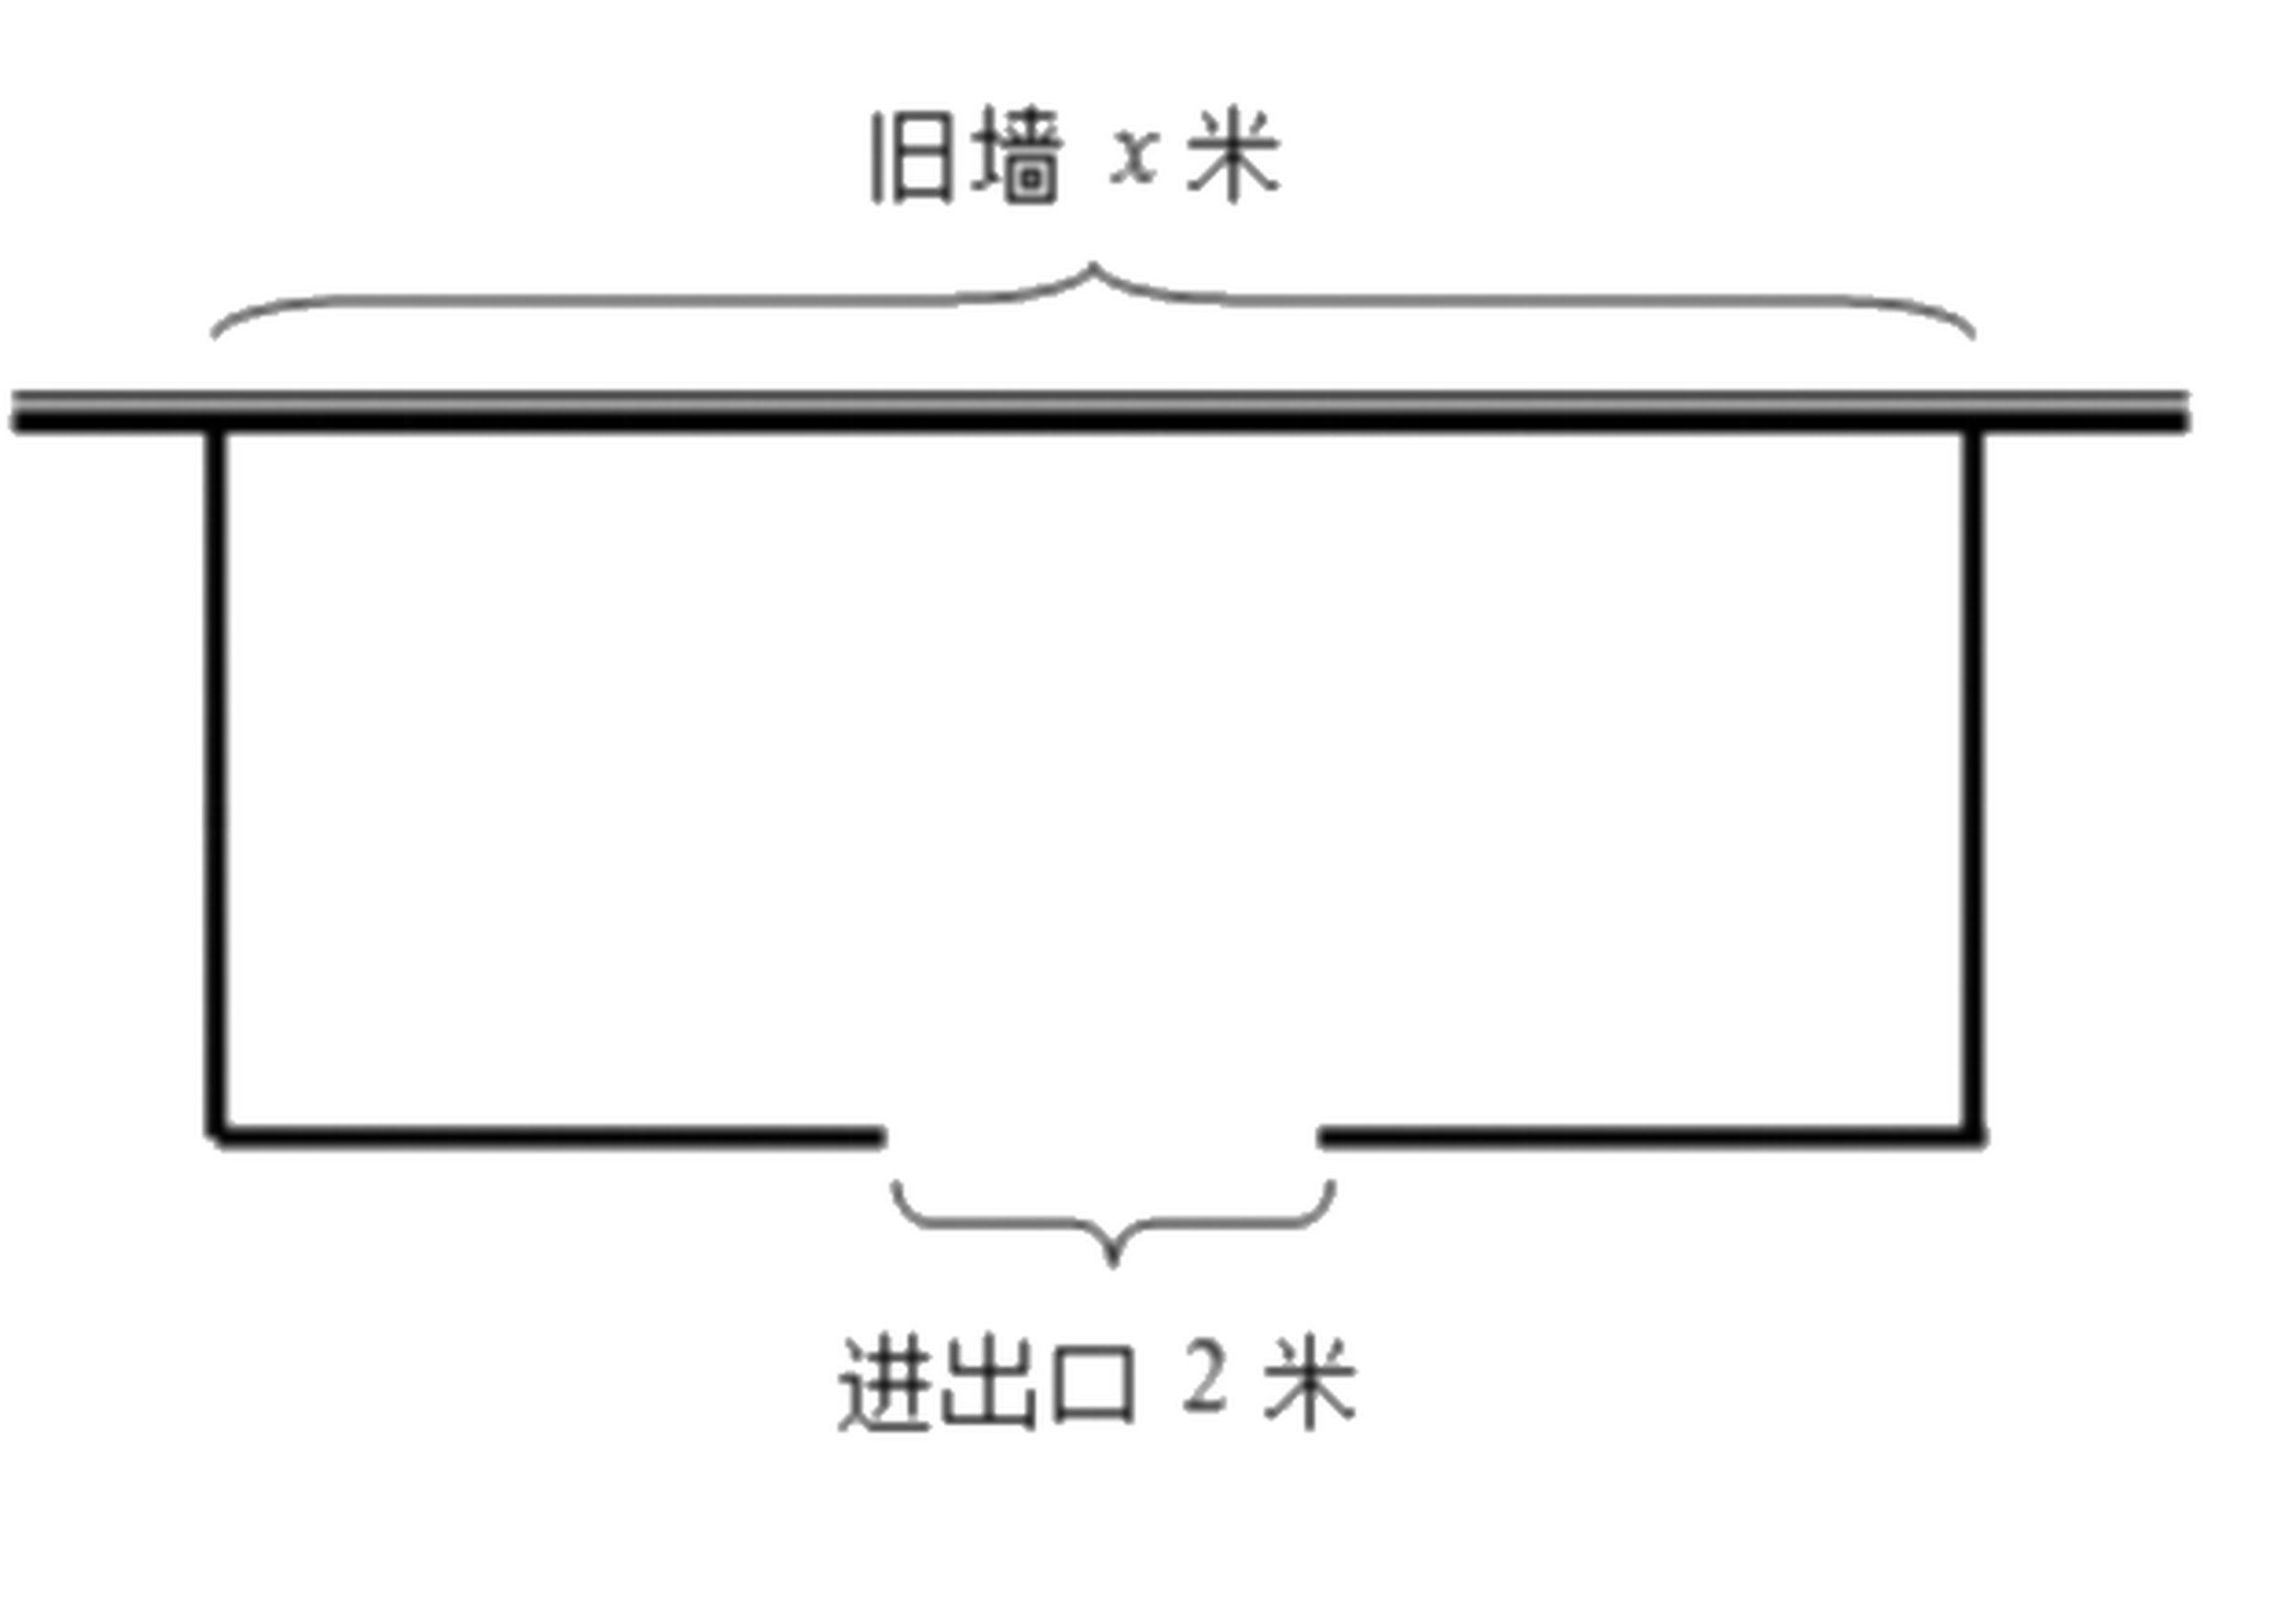
\includegraphics[width=0.60\textwidth]{figures/gao144_q17.png}
\end{center}

(1) 写出总费用 $y$ 关于 $x$ 的表达式;

(2) 试确定 $x$，使修建此矩形场地围墙的总费用最小，并求出最小总费用.

\ifanswer
\solbegin
\step{(1) 设矩形的另一边长为 $a$ 米，}
\step{则 $y=45x+180(x-2)+180\times2a=225x+360a-360$，}
\step{由已知 $xa=360$，得 $a=\dfrac{360}{x}$，所以 $y=225x+\dfrac{360^2}{x}-360(x>0)$;}
\step{(2) 因为 $x>0$，所以 $225x+\dfrac{360^2}{x}\geqslant2\sqrt{225x\cdot\dfrac{360^2}{x}}=10800$，}
\step{所以 $y=225x+\dfrac{360^2}{x}-360\geqslant10440$，}
\step{当且仅当 $225x=\dfrac{360^2}{x}$，即 $x=24$ 时取等号，}
\step{所以当 $x=24$ 米时，修建围墙的总费用最小，最小总费用是 10440 元.}
\solend
\fi

\item 已知集合 $A=\{a_1,a_2,\cdots,a_k\}(k\geqslant2)$，其中 $a_i\in\Z(i=1,2,\cdots,k)$. 定义：若对任意的 $x\in A$，必有 $-x\notin A$，则称集合 $A$ 具有性质 $G$. 由 $A$ 中元素可构成两个点集 $P$ 和 $Q$，$P=\{(x,y)\mid x\in A,y\in A,x+y\in A\}$，$Q=\{(x,y)\mid x\in A,y\in A,x-y\in A\}$，其中 $P$ 有 $m$ 个元素，$Q$ 中有 $n$ 个元素.

(1) 已知集合 $K=\{-1,2,3\}$，判断 $K$ 是否具有性质 $G$; 并写出 $K$ 对应的集合 $P$ 和集合 $Q$;

(2) 若集合 $A=\{1,2,3,4,5,6,7,8,9,10\}$，求对应集合 $Q$ 的元素个数; 一般地，若集合 $A$ 具有性质 $G$，且有 $k$ 个元素，猜测对应的集合 $Q$ 的元素最大个数，并说明理由;

(3) 若集合 $A$ 具有性质 $G$，猜测 $m,n$ 的大小并说明理由.

\ifanswer
\solbegin
\step{(1) 因为 $K=\{-1,2,3\},1,-2,-3$ 都不属于集合 $K$，}
\step{所以集合 $K$ 具有性质 $G$，}
\step{对应集合 $P=\{(-1,3),(3,-1)\},Q=\{(2,-1),(2,3)\}$;}
\step{(2) $A=\{1,2,3,4,5,6,7,8,9,10\}$，则对应集合 $Q$ 中的元素为:}
\step{$(2,1),(3,2),\cdots,(9,8),(10,9)$,}
\step{$(3,1),(4,2),\cdots,(9,7),(10,8)$,}
\step{$(4,1),(5,2),\cdots,(9,6),(10,7)$,}
\step{$\cdots$}
\step{$(9,1),(10,2)$,}
\step{$(10,1)$,}
\step{共有 $9+8+7+\cdots+2+1=45$ 个元素，即对应集合 $Q$ 的元素个数 45;}
\step{集合 $A$ 有 $k$ 个元素，猜测对应的集合 $Q$ 的最大个数为 $\dfrac{k^2-k}{2}$. 理由如下:}
\step{由题意得集合 $A$ 的元素构成有序数对 $(a_i,a_j)(i,j\in\N^*,i\leqslant k,j\leqslant k)$，}
\step{共有 $k^2$ 个，因为 $0\notin A$，所以 $(a_i,a_i)\notin Q$，}
\step{又因为 $a\in A$ 时，$-a\notin A$，所以 $(a_i,a_j)\in Q$ 时，$(a_j,a_i)\notin Q$，}
\step{所以集合 $Q$ 的元素个数为 $\dfrac{k^2-k}{2}$ 个，}
\step{(3) 当集合 $A$ 具有性质 $G$ 时，}
\step{①对于 $(a,b)\in P$，由定义得 $a\in A,b\in A,a+b\in A$，}
\step{又因为集合 $A$ 具有性质 $G$，所以 $(a+b,a)\in Q$，}
\step{如果 $(a,b),(c,d)$ 是 $P$ 中的不同元素，}
\step{那么 $a=c,b=d$ 中至少有一个不成立，}
\step{于是 $b=d,a+b=c+d$ 中至少有一个不成立，}
\step{故 $(a+b,b)$ 和 $(c+d,d)$ 也是 $Q$ 中不同的元素，}
\step{可见 $P$ 的元素个数不多于 $Q$ 的元素个数，即 $m\leqslant n$;}
\step{②对于 $(a,b)\in Q$，由定义得 $a\in A,b\in A,a-b\in A$，}
\step{又因为集合 $A$ 具有性质 $G$，则 $(a-b,b)\in P$，}
\step{如果 $(a,b),(c,d)$ 是 $Q$ 中的不同元素，}
\step{那么 $a=c,b=d$ 中至少有一个不成立，}
\step{于是 $b=d,a-b=c-d$ 中至少有一个不成立，}
\step{故 $(a-b,b)$ 和 $(c-d,d)$ 也是 $P$ 中不同的元素，}
\step{可见 $Q$ 的元素个数不多于 $P$ 的元素个数，即 $n\leqslant m$，}
\step{由①②得 $m=n$.}
\solend
\fi

\end{enumerate}

\end{document}
"
%
% ① 原始材料：微信公众号"魔都数学加油站"文章，连载"27学年高一144"，原文标题
% "27学年高一144——2026-2027年上海市风华中学高一上期中"；
% 原文链接：https://mp.weixin.qq.com/s/ylUlbXfudWOYC-jlH3jyjw 。
% 正文为 10 张 PNG 页，题目下印【解析】，为讲评版。
% 各页分辨率：01/02/03/05/06/07/09/10 为 2560×3620，04/08 为 4762×6735。
% 题目、解析均据原图转录；卷面粉红色水印"魔都数学加油站"及公众号页脚未录入。
% 全卷插图情况：Q17 有一幅矩形场地示意图（旧墙 x 米 / 进出口 2 米），从 07 页裁出、
%   去粉色水印去色 4× LANCZOS 放大存 figures/gao144_q17.png；其余 9 页逐页通读
%   确认无题目配图、无表格、亦无"题干写如图而源码漏图"一处。
%
% 卷首标题：原卷印作"2026-2027 年风华中学高一上期中"，年份区间按全稿惯例排 en dash；
% 原卷卷面未印副标题，本稿按同期中卷（高一140／141／143）知识模块口径补出
% "集合与常用逻辑用语、不等式、函数"：集合与逻辑见 Q3、Q7、Q9、Q10、Q12、Q16、Q18，
% 不等式见 Q6、Q11、Q13、Q14、Q15、Q17，函数见 Q4、Q5、Q8、Q9。
%
% 题号体例：本卷共 16 题——一、填空题 3—10（8 题）、二、选择题 11—13（3 题）、
% 三、解答题 14—18（5 题）。三节分别 \setcounter{enumi}{2}／{10}／{13}。
% 原卷从第 3 题起、无第 1、2 题，本稿保留原题号；全卷无附加题节。
%
% ② 与原卷的排版差异：
%   ① 原文从第 3 题起，本稿保留原题号；共 16 题三节；
%   ② 原卷 15 题题下印【解析】，唯 Q11 未印【解析】、只把答案"（ BD ）"直接印在
%      题干括号内（放大 04 页 A/B 选项与 05 页 C/D 选项衔接处确认，见 ⑤）；
%      按 高一128／94／106／140 成例：Q11 试卷版括号留空 \mbox{（\quad）}、
%      答案版另提 \ans{$BD$}、不补造原卷没有的解析；其余 15 题印【解析】、
%      括号内一律留空、不另提 \ans{}（Q12 选 C、Q13 选 B 在解析末句"故选 …"）；
%      答案版【答案】/【解析】标记数 = 16（1 个 \ans + 15 个 \solbegin）= 全卷题数；
%      正文 Q11 对应处另有 % 注；
%   ③ 原卷卷面未印副标题，本稿按知识模块口径补出；
%   ④ 原卷填空横线按全稿惯例排 \blankline[4.4em]；选择题括号排 \mbox{（\quad）}，
%      选项段前按惯例加 \keepwithprev；解答题不留作答区、不加 \anspace
%      （原卷为讲评版，与 129／131／132／133／136／140／141／143 同）；
%   ⑤ 数集：Q9 题干与解析"a,b∈R"、Q12 题干"U=R"、Q15 题干"x,y∈R"原卷印
%      斜体或黑板粗体 R，Q18 题干"a_i∈Z"印黑板粗体 Z、Q18 解析"i,j∈N*"印
%      黑板粗体 N，按全稿惯例统一改 \R／\Z／\N^*；绝对值排 \lvert…\rvert，
%      集合描述竖线排 \mid；不等号按全稿惯例排 \leqslant／\geqslant；
%      补集照原卷上划线排 \overline{A}／\overline{B}；空集记号 \varnothing；
%   ⑥ 子题标号 (1)(2)(3) 原卷印半角括号，照录；圈数字 ①② 在正文（文本模式）
%      按原卷照录（Q15、Q18 解析），未进数学式；数学式内半角逗号照录
%      （Q12 解析"$A=(1,2),B=(0,6)$"、Q18 解析"$(a_i,a_j)(i,j\in\N^*,i\leqslant k,j\leqslant k)$"、
%      Q15 解析"$x=1,y=-1$"、Q18 解析"$a=c,b=d$"等，为全稿惯例、非笔误）；
%      全卷行末西文句点照录为 ASCII `.`；行中全角逗号／顿号照录；
%      Q18 解析集合描述中的"或"用 \text{ 或 } 置于数学式内；
%   ⑦ 题干中的中文弯引号按原卷照录（Q3 的" x∈A "／" x∈B "与 Q15 (2) 的命题
%      引号，含引号内空格），注释内一律 ASCII 引号；
%   ⑧ Q17 配图：题干写"如图所示"，配图居中排在题干之后、子问之前，三版都出；
%      在 Q17 \item 之前加 \needvspace{10cm} 把"题干＋图"整块推走。Q17 是
%      "三、解答题"节内第 4 题（非节首题），故守卫放在 \item 之前而非 \bigsec
%      之前不会让节标题孤落页末（B 类）；三版切页审计均"合计异常：无"；
%   ⑨ 跨页续印按题合并：Q3 在 01 页；Q4/5/6 在 01 页（Q6 解析续到 02 页顶）；
%      Q7/8/9 在 02 页（Q9 题干跨 02→03）；Q10 在 03 页、解析跨 03→04（很长，
%      按余数分组 A₁/A₂/A₃）；Q11 在 04 页（"二、选择题"节标题也在 04 页下部）、
%      Q12/13 在 05 页（"三、解答题"标题在 05 页下部）；Q14 在 05 页末、解析在 06 页；
%      Q15/16 在 06 页（Q16 续到 07 页）；Q17 在 07 页；Q18 在 08 页、解析跨
%      08/09/10 页（性质 G 压轴，3 问，很长）；本稿按题连排，不丢行、不并折行；
%   ⑩ Q8 解析"法一：""法二："两处标签经放大 02 页逐字确认原卷均印红色
%      （见 ⑤）；按全稿惯例（高一53 成例）不引入红色、均照录为黑体着色
%      \stepm{法一：}{…}／\stepm{法二：}{…}，不改 common.sty；
%      文件头在此注明原卷为红色；
%   ⑪ "图像／图象"逐处核：全卷未出现"图像"或"图象"字样，无统一问题；
%   ⑫ \left…\right 不得拆到不同 $…$ 组；cases 块整体算一个印刷行；
%      Q4 分式与 8×(-3/4) 同一 $…$ 组，Q13 的 \left(\frac1x+\frac2y\right) 同理。
%
% ③ 行数复核：一条 \step／\stepm 行 = 原卷解析的一个印刷行，cases 块作一个印刷行计。
%   逐题数（含 \stepm）：Q3：3；Q4：1；Q5：1；Q6：5；Q7：4；Q8：8（6 \step
%   ＋ 2 \stepm，法一/法二标签各占 1 行）；Q9：6；Q10：23；Q11：0（原卷无解析，
%   答案另提 \ans{$BD$}）；Q12：5；Q13：3；Q14：5；Q15：8；Q16：7；Q17：7；
%   Q18：32。合计 116 条 \step ＋ 2 条 \stepm ＝ 118 个印刷行，与原卷逐题相等。
%   全卷 15 题设 \solbegin…\solend ＋ Q11 一处 \ans{}，答案版【答案】/【解析】
%   标记数 = 16 = 全卷题数。
%
% ④ 判别式／子集符号结论（逐处放大原图照录、不得统一）：
%   判别式全卷 2 处，逐页放大扫过 10 页确认（Q4 为分式指数化简、不含判别式）：
%     · Q9【解析】"所以 △=a^2-4b=0" 原卷印细线、扁等边三角（宽≈高、笔画细，
%       放大见 /tmp/gao144fh/z_q9_tri.png、z_tri_Q9.png），照录 \triangle；
%     · Q15 (2)【解析】cases 块"Δ=(a-2)^2-4(a-2)≤0" 原卷印等腰偏高、粗笔画
%       三角（高>宽，放大见 z_q15_tri.png、z_tri_Q15.png），照录 \Delta；
%   两形不同、全卷混用，逐处照录不统一（参照 高一142 头注④口径）。
%   子集符号全卷 4 处，逐处放大核：
%     · Q3 解析"所以 B⊆A"、Q16 (1) 解析"所以 B⊆A" 原卷均印带下划线的 ⊆
%       （z_q3_symbol.png、z_q16_subset2.png），照录 \subseteq；
%     · Q12 选项 B"$\overline{A}\subset B$" 原卷印单线 ⊂（z_q12_opts2.png），
%       照录 \subset；Q12 解析"$\overline{A}=(-\infty,1]\cup[2,+\infty)\not\subset B$"
%       原卷印单线带斜杠 ⊄（z_q12_notsym3.png），照录 \not\subset；
%   \subset 与 \subseteq 混用，逐处照录不统一。补集照原卷上划线 \overline{A}／
%   \overline{B}，空集 \varnothing，数集 \R／\Z／\N^* 归一见 ② ⑤。
%
% ⑤ 存疑／特殊体例（主会话逐处放大原图复核确认，照录未改，正文对应处另有 % 注）：
%   1. 第 11 题原卷把答案"（ BD ）"直接印在题干括号内、题下未印【解析】
%      （放大 04 页 A/B 选项与 05 页 C/D 选项衔接处确认：05 页顶 C/D 选项后
%      直接接第 12 题）。按 高一128／94／106／140 成例括号留空、另提
%      \ans{$BD$}，不补造解析（不编造）。
%   2. 第 10 题题干"集合 $S$ 为集合 $M=\{1,2,3,4,\cdots,2026\}$，的子集"在
%      集括号与"的子集"之间原卷多印一个全角逗号（放大 03 页确认），
%      按存疑照录未删，正文对应处另有 % 注。
%   3. 第 8 题解析"法一：""法二："两处原卷均印红色（放大 02 页逐字确认），
%      按全稿惯例不引入红色、两处均照录为黑体着色 \stepm（见 ② ⑩）。
%   全卷除此 3 条外未发现其它笔误／自相矛盾处。
%
% ⑥ 跨页续印按题合并说明：见 ② ⑨。
%
\documentclass[a4paper,11pt]{article}
\usepackage{common}

\begin{document}

\examtitlest[3]{2026--2027 年风华中学高一上期中}{集合与常用逻辑用语、不等式、函数}

\bigsec{一、填空题}

\begin{enumerate}
\setcounter{enumi}{2}

\item $A=\{x\mid x>4\}$，$B=\{x\mid x>a\}$，若命题 “ $x\in A$ ” 是命题 “ $x\in B$ ” 的必要条件，则 $a$ 的取值范围是\blankline[4.4em].

\ifanswer
\solbegin
\step{因为 “ $x\in A$ ” 是命题 “ $x\in B$ ” 的必要条件，所以 $B\subseteq A$，}% 子集符号原卷印带下划线 $\subseteq$，照录
\step{因为 $A=\{x\mid x>4\}$，$B=\{x\mid x>a\}$，所以 $a\geqslant4$，}
\step{所以 $a$ 的取值范围是 $\{a\mid a\geqslant4\}$.}
\solend
\fi

\item 已知 $a>0,b>0$，化简式子：$\dfrac{8a^{\frac34}b^3}{\left(a^{\frac16}b^{\frac32}\right)\left(-\dfrac43 a^{\frac1{12}}b^{\frac12}\right)}=$\blankline[4.4em].

\ifanswer
\solbegin
\step{$\dfrac{8a^{\frac34}b^3}{\left(a^{\frac16}b^{\frac32}\right)\left(-\dfrac43 a^{\frac1{12}}b^{\frac12}\right)}=8\times\left(-\dfrac34\right)a^{\frac34-\frac16-\frac1{12}}b^{3-\frac32-\frac12}=-6a^{\frac12}b=-6b\sqrt a$.}
\solend
\fi

\item 已知 $\lg2=a$，$\lg3=b$，则 $\log_5 6=$\blankline[4.4em]（结果用 $a,b$ 表示）.

\ifanswer
\solbegin
\step{$\log_5 6=\dfrac{\lg6}{\lg5}=\dfrac{\lg2+\lg3}{1-\lg2}=\dfrac{a+b}{1-a}$.}
\solend
\fi

\item 若关于 $x$ 的不等式 $ax>b$ 的解集为 $(-\infty,2)$，则不等式 $bx+a>0$ 的解集为\blankline[4.4em].

\ifanswer
\solbegin
\step{因为不等式 $ax>b$ 的解集为 $(-\infty,2)$，所以 $a<0$，}
\step{所以由不等式解得 $x<\dfrac ba$，所以 $\dfrac ba=2$，即 $b=2a$，}
\step{代入不等式 $bx+a>0$，得 $2ax+a>0$，}
\step{因为 $a<0$，所以不等式化为 $2x+1<0$，解得 $x<-\dfrac12$，}
\step{故不等式的解集为 $\left(-\infty,-\dfrac12\right)$.}
\solend
\fi

\item 如果集合 $A=\{x\mid x^2-4x\leqslant0\}$，$B=\{x\mid x^2+ax+b\leqslant0\}$，$A\cap B=\{x\mid3\leqslant x\leqslant4\}$，$A\cup B=\{x\mid0\leqslant x\leqslant5\}$，则 $a+b=$\blankline[4.4em].

\ifanswer
\solbegin
\step{由题意得 $A=\{x\mid x^2-4x\leqslant0\}=[0,4]$，}
\step{又因为 $A\cap B=\{x\mid3\leqslant x\leqslant4\}$，$A\cup B=\{x\mid0\leqslant x\leqslant5\}$，}
\step{所以 $B=\{x\mid3\leqslant x\leqslant5\}$，即方程 $x^2+ax+b=0$ 的两根为 $3,5$，}
\step{由韦达定理得 $\begin{cases}3+5=-a\\3\times5=b\end{cases}$，解得 $a=-8$，$b=15$，所以 $a+b=15-8=7$.}
\solend
\fi

% 第 8 题：原卷"法一：""法二："两处标签均印红色（8× 放大确认）；按交办口径
% "法一"用普通 \step、"法二："排 \stepm（加粗着色、不引红色），见头注 ② ⑩／⑤
\item 若关于 $x$ 的方程 $\lvert x-1\rvert+\lvert\pi-x\rvert=\pi-1$ 的解集为\blankline[4.4em].

\ifanswer
\solbegin
\stepm{法一：}{因为 $\lvert x-1\rvert+\lvert\pi-x\rvert=\begin{cases}x-1+x-\pi,x\geqslant\pi\\\pi-1,1<x<\pi\\1-x+\pi-x,x\leqslant1\end{cases}=\begin{cases}2x-1-\pi,x\geqslant\pi\\\pi-1,1<x<\pi\\1+\pi-2x,x\leqslant1\end{cases}$.}
\step{当 $x\geqslant\pi$ 时，令 $2x-1-\pi=\pi-1$，得 $x=\pi$；}
\step{当 $1<x<\pi$ 时，$\lvert x-1\rvert+\lvert\pi-x\rvert=\pi-1$ 恒成立；}
\step{当 $x\leqslant1$ 时，令 $1+\pi-2x=\pi-1$，得 $x=1$.}
\step{综上所述，方程 $\lvert x-1\rvert+\lvert\pi-x\rvert=\pi-1$ 的解集为 $[1,\pi]$.}
\stepm{法二：}{因为 $\lvert x-1\rvert+\lvert\pi-x\rvert\geqslant\lvert x-1+\pi-x\rvert=\pi-1$，}
\step{当且仅当 $(x-1)(\pi-x)\geqslant0$ 时取等号，}
\step{故方程 $\lvert x-1\rvert+\lvert\pi-x\rvert=\pi-1$ 的解集为 $[1,\pi]$.}
\solend
\fi

% 第 9 题：题干跨 02→03 页；解析判别式原卷印细线扁等边三角 $\triangle$，照录
\item 已知函数 $f(x)=x^2+ax+b(a,b\in\R)$ 和 $x$ 轴有且只有一个交点，若关于 $x$ 的不等式 $f(x)<c$ 的解集为 $(m,m+6)$，则 $c=$\blankline[4.4em].

\ifanswer
\solbegin
\step{因为函数 $f(x)=x^2+ax+b(a,b\in\R)$ 和 $x$ 轴有且只有一个交点，}
\step{所以 $\triangle=a^2-4b=0$，即 $b=\dfrac{a^2}{4}$，}% 判别式原卷印扁等边三角 $\triangle$，照录
\step{不等式 $f(x)<c$ 的解集为 $(m,m+6)$，}
\step{即 $x^2+ax+\dfrac{a^2}{4}-c<0$ 的解集为 $(m,m+6)$，}
\step{所以方程 $x^2+ax+\dfrac{a^2}{4}-c=0$ 的两个根为 $x_1=m$，$x_2=m+6$，}
\step{所以 $\begin{cases}x_1+x_2=2m+6=-a\\x_1x_2=m(m+6)=\dfrac{a^2}{4}-c\end{cases}$，消去 $m$ 得 $\dfrac{a^2}{4}-9=\dfrac{a^2}{4}-c$，解得 $c=9$.}
\solend
\fi

% 第 10 题：原卷题干在集括号与"的子集"之间多印一个全角逗号，照录未改（存疑，见头注 ⑤）
\item 已知集合 $S$ 为集合 $M=\{1,2,3,4,\cdots,2026\}$，的子集，并且集合 $S$ 中任意两个元素之和不能被 3 整除，则集合 $S$ 中元素个数的最大值为\blankline[4.4em].

\ifanswer
\solbegin
\step{对于集合 $M=\{1,2,3,4,\cdots,2026\}$，}
\step{所有被 3 除余数为 0 的元素组成的集合为 $A_3=\{3,6,9,\cdots,2025\}$，}
\step{元素个数为 675;}
\step{所有被 3 除余数为 1 的元素组成的集合为 $A_1=\{1,4,7,\cdots,2026\}$，}
\step{元素个数为 676;}
\step{所有被 3 除余数为 2 的元素组成的集合为 $A_2=\{2,5,8,\cdots,2024\}$，}
\step{元素个数为 675;}
\step{集合 $S$ 中任意两个元素之和不能被 3 整除，}
\step{若两个元素分别来自 $A_1$ 和 $A_2$，则两数之和除以 3 的余数为 $1+2=3\equiv0$，}
\step{即和能被 3 整除，}
\step{所以 $S$ 不能同时包含 $A_1$ 和 $A_2$ 中的元素，}
\step{即 $S$ 最多只能选取 $A_1$、$A_2$ 一个集合中的全部元素;}
\step{若两个元素都来自 $A_3$，则两数之和除以 3 的余数为 $0+0=0$，即和能被 3 整除，}
\step{所以 $S$ 中最多包含 $A_3$ 中的 1 个元素;}
\step{对 $A_1$ 内的任意两个元素，其和除以 3 的余数为 $1+1=2$，不能被 3 整除;}
\step{$A_1$ 中元素与 $A_3$ 中元素的和除以 3 余数为 $1+0=1$，不能被 3 整除，}
\step{所以 $A_1$ 的全部元素与 $A_3$ 中的任意 1 个元素的组合满足题意;}
\step{对 $A_2$ 内的任意两个元素，其和除以 3 的余数为 $2+2=4\equiv1$，不能被 3 整除;}
\step{$A_2$ 中元素与 $A_3$ 中元素的和除以 3 的余数为 $2+0=2$，不能被 3 整除，}
\step{所以 $A_2$ 的全部元素与 $A_3$ 中任意 1 个元素的组合也满足题意.}
\step{故若选取 $A_2$ 全部元素加 1 个 $A_3$ 元素，总个数为 $675+1=676$;}
\step{选取 $A_1$ 全部元素加 1 个 $A_3$ 元素，总个数为 $676+1=677$;}
\step{所以集合 $S$ 中元素个数的最大值为 677.}
\solend
\fi

\end{enumerate}

\bigsec{二、选择题}

\begin{enumerate}
\setcounter{enumi}{10}

% 第 11 题：原卷把答案"（ BD ）"直接印在题干括号内、题下无【解析】（放大 04 页 A/B 选项
% 与 05 页 C/D 选项衔接处确认）。按 高一128／94／106／140 成例：试卷版括号留空、
% 答案版另提 \ans{$BD$}、不补造原卷没有的解析（不编造）。
\item 已知实数 $a,b$，下列四个不等式中正确的是\mbox{（\quad）}

\keepwithprev
A. $a+\dfrac1a\geqslant2$\qquad B. $\sqrt{a^2+2}+\dfrac{1}{\sqrt{a^2+2}}\geqslant2$

C. $\dfrac{a+b}{2}\leqslant\sqrt{ab}$\qquad D. $a^2+b^2\geqslant2ab$

\ifanswer
\ans{$BD$}
\fi

\item 若全集 $U=\R$，$A=\{x\mid x^2-3x+2<0\}$，$B=\{x\mid0<x<6\}$，则\mbox{（\quad）}

\keepwithprev
A. $A\cap B=B$\qquad B. $\overline{A}\subset B$\qquad C. $A\cap\overline{B}=\varnothing$\qquad D. $A\cup B=A$

\ifanswer
\solbegin
\step{由 $x^2-3x+2<0$，则 $A=(1,2),B=(0,6)$，所以 $A\cap B=(1,2)=A,A$ 错误;}
\step{$\overline{A}=(-\infty,1]\cup[2,+\infty)\not\subset B$，$B$ 错误;}
\step{$\overline{B}=(-\infty,0]\cup[6,+\infty)$，所以 $A\cap\overline{B}=\varnothing,C$ 正确;}
\step{$A\cup B=(0,6)\ne A,D$ 错误.}
\step{故选 $C$.}
\solend
\fi

\item 已知正数 $x$、$y$ 满足 $\dfrac1x+\dfrac2y=1$，不等式 $3x+2y-1>m$ 恒成立，则实数 $m$ 的取值范围是\mbox{（\quad）}

\keepwithprev
A. $(-\infty,4+6\sqrt2)$\qquad B. $(-\infty,6+4\sqrt3)$\qquad C. $(6+4\sqrt2,+\infty)$\qquad D. $(8+4\sqrt3,+\infty)$

\ifanswer
\solbegin
\step{$3x+2y=(3x+2y)\left(\dfrac1x+\dfrac2y\right)=7+\dfrac{6x}{y}+\dfrac{2y}{x}\geqslant7+2\sqrt{\dfrac{6x}{y}\cdot\dfrac{2y}{x}}=7+4\sqrt3$，}
\step{当且仅当 $\dfrac{6x}{y}=\dfrac{2y}{x}$，即 $y=\sqrt3x=\sqrt3+2$ 时取等号，}
\step{故要使原式成立，只需 $m<6+4\sqrt3$. 故选 $B$.}
\solend
\fi

\end{enumerate}

\bigsec{三、解答题}

\begin{enumerate}
\setcounter{enumi}{13}

\item 解关于 $x$ 的不等式：

(1) $x^2-2\lvert x\rvert-3>0$；

(2) $\dfrac{2x-1}{x+2}<1$.

\ifanswer
\solbegin
\step{(1) 原不等式等价于 $(\lvert x\rvert-3)(\lvert x\rvert+1)>0$，}
\step{$\lvert x\rvert+1>0$，故 $\lvert x\rvert>3$，解得 $x<-3$ 或 $x>3$，}
\step{故不等式的解集为 $(-\infty,-3)\cup(3,+\infty)$.}
\step{(2) 已知 $\dfrac{2x-1}{x+2}<1$，则 $\dfrac{2x-1}{x+2}-1<0$，即 $\dfrac{x-3}{x+2}<0$，}
\step{等价于 $(x-3)(x+2)<0$，解得 $-2<x<3$，故不等式的解集为 $(-2,3)$.}
\solend
\fi

\item (1) 已知 $x,y\in\R$，比较 $x^2+y^2$ 与 $2x-2y-2$ 的大小.

(2) “不等式 $(a-2)x^2+(a-2)x+1\geqslant0$ 对一切实数恒成立” 是假命题，求实数 $a$ 的取值范围.

\ifanswer
\solbegin
\step{(1) $x^2+y^2-(2x-2y-2)=x^2+y^2-2x+2y+2=(x-1)^2+(y+1)^2\geqslant0$，}
\step{故 $x^2+y^2\geqslant2x-2y-2$，当且仅当 $x=1,y=-1$ 时取等号.}
\step{(2) 先求命题 “$(a-2)x^2+(a-2)x+1\geqslant0$ 对一切实数恒成立” 为真，}
\step{①当 $a-2=0$ 时，即 $a=2$，不等式化为 $1\geqslant0$，成立，符合条件，}
\step{②当 $a-2\ne0$ 时，则 $\begin{cases}a-2>0\\\Delta=(a-2)^2-4(a-2)\leqslant0\end{cases}$，解得 $2<a\leqslant6$，}% 判别式原卷印等腰偏高三角 $\Delta$，照录
\step{综上①②，命题为真时 $2\leqslant a\leqslant6$，}
\step{该命题为假命题，则 $a<2$ 或 $a>6$，}
\step{所以实数 $a$ 的取值范围是 $(-\infty,2)\cup(6,+\infty)$.}
\solend
\fi

\item 设集合 $A=\{x\mid-1\leqslant x\leqslant2\}$，$B=\{x\mid m-1<x<2m+1\}$.

(1) 若 $A\cup B=A$，求实数 $m$ 的取值范围;

(2) 若 $B\cap\overline{A}$ 中只有一个整数 $-2$，求实数 $m$ 的取值范围.

\ifanswer
\solbegin
\step{(1) 因为 $A\cup B=A$，所以 $B\subseteq A$，}% 子集符号原卷印带下划线 $\subseteq$，照录
\step{当 $B=\varnothing$ 时，有 $m-1\geqslant2m+1$，解得 $m\leqslant-2$；}
\step{当 $B\ne\varnothing$ 时，有 $\begin{cases}m-1<2m+1\\m-1\geqslant-1\\2m+1\leqslant2\end{cases}$，解得 $0\leqslant m\leqslant\dfrac12$，}
\step{所以实数 $m$ 的取值范围是 $(-\infty,-2]\cup\left[0,\dfrac12\right]$;}
\step{(2) 由集合 $A=\{x\mid-1\leqslant x\leqslant2\}$，得 $\overline{A}=\{x\mid x<-1\text{ 或 }x>2\}$，}
\step{若 $B\cap\overline{A}$ 中只有一个整数 $-2$，则 $B\ne\varnothing$，且满足 $\begin{cases}m-1<2m+1\\-3\leqslant m-1<-2\\-2<2m+1\leqslant3\end{cases}$}
\step{解得 $-\dfrac32<m<-1$，所以实数 $m$ 的取值范围是 $\left(-\dfrac32,-1\right)$.}
\solend
\fi

% 第 17 题配图是"题干＋图"整块；守卫放在 \item 之前（Q17 非节首题，不会让节标题孤落页末）
\needvspace{10cm}
\item 现要围建一个面积为 360 平方米的矩形场地，要求矩形场地的一面利用旧墙（利用旧墙需维修），其它三面围墙要新建，在旧墙的对面的新墙上要留一个宽度为 2 米的进出口，如图所示，已知旧墙的维修费用为 45 元/米，新墙的造价为 180 元/米，设利用的旧墙的长度为 $x$ 米，工程总造价为 $y$（单位：元）.

\begin{center}
% 矩形场地示意图取自 07 页右侧，去粉色水印、去色、4× LANCZOS 放大
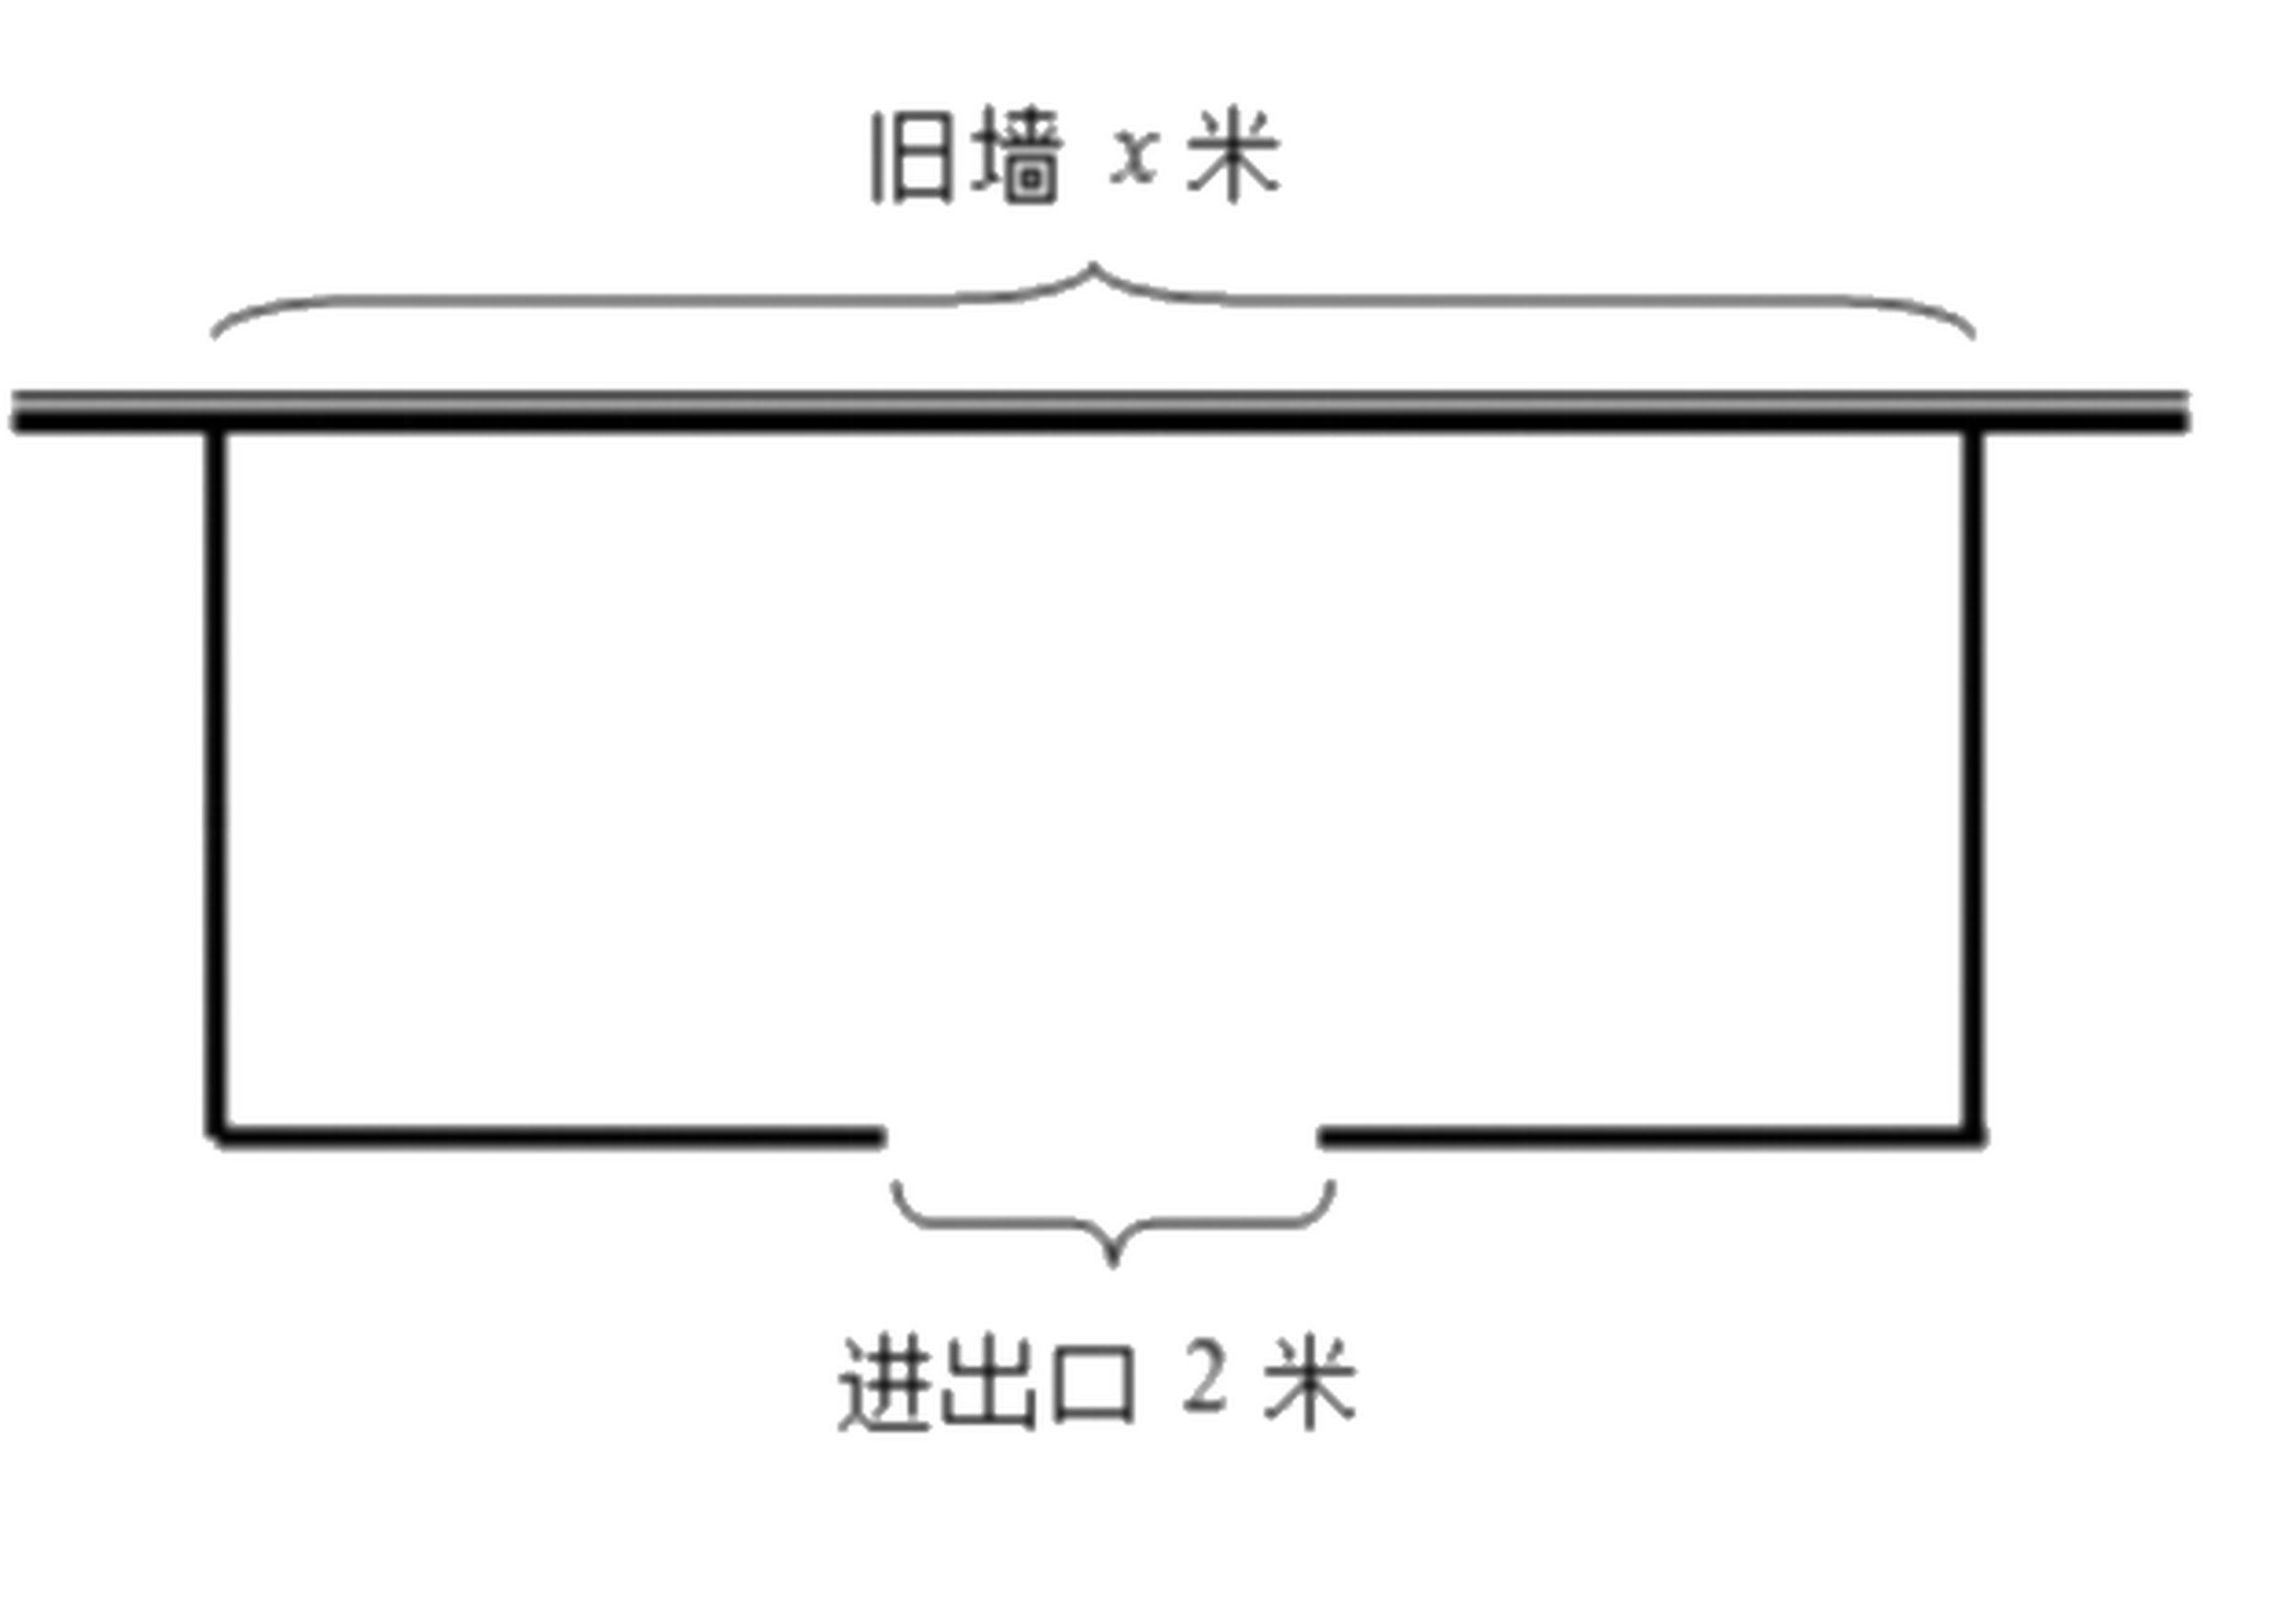
\includegraphics[width=0.60\textwidth]{figures/gao144_q17.png}
\end{center}

(1) 写出总费用 $y$ 关于 $x$ 的表达式;

(2) 试确定 $x$，使修建此矩形场地围墙的总费用最小，并求出最小总费用.

\ifanswer
\solbegin
\step{(1) 设矩形的另一边长为 $a$ 米，}
\step{则 $y=45x+180(x-2)+180\times2a=225x+360a-360$，}
\step{由已知 $xa=360$，得 $a=\dfrac{360}{x}$，所以 $y=225x+\dfrac{360^2}{x}-360(x>0)$;}
\step{(2) 因为 $x>0$，所以 $225x+\dfrac{360^2}{x}\geqslant2\sqrt{225x\cdot\dfrac{360^2}{x}}=10800$，}
\step{所以 $y=225x+\dfrac{360^2}{x}-360\geqslant10440$，}
\step{当且仅当 $225x=\dfrac{360^2}{x}$，即 $x=24$ 时取等号，}
\step{所以当 $x=24$ 米时，修建围墙的总费用最小，最小总费用是 10440 元.}
\solend
\fi

\item 已知集合 $A=\{a_1,a_2,\cdots,a_k\}(k\geqslant2)$，其中 $a_i\in\Z(i=1,2,\cdots,k)$. 定义：若对任意的 $x\in A$，必有 $-x\notin A$，则称集合 $A$ 具有性质 $G$. 由 $A$ 中元素可构成两个点集 $P$ 和 $Q$，$P=\{(x,y)\mid x\in A,y\in A,x+y\in A\}$，$Q=\{(x,y)\mid x\in A,y\in A,x-y\in A\}$，其中 $P$ 有 $m$ 个元素，$Q$ 中有 $n$ 个元素.

(1) 已知集合 $K=\{-1,2,3\}$，判断 $K$ 是否具有性质 $G$; 并写出 $K$ 对应的集合 $P$ 和集合 $Q$;

(2) 若集合 $A=\{1,2,3,4,5,6,7,8,9,10\}$，求对应集合 $Q$ 的元素个数; 一般地，若集合 $A$ 具有性质 $G$，且有 $k$ 个元素，猜测对应的集合 $Q$ 的元素最大个数，并说明理由;

(3) 若集合 $A$ 具有性质 $G$，猜测 $m,n$ 的大小并说明理由.

\ifanswer
\solbegin
\step{(1) 因为 $K=\{-1,2,3\},1,-2,-3$ 都不属于集合 $K$，}
\step{所以集合 $K$ 具有性质 $G$，}
\step{对应集合 $P=\{(-1,3),(3,-1)\},Q=\{(2,-1),(2,3)\}$;}
\step{(2) $A=\{1,2,3,4,5,6,7,8,9,10\}$，则对应集合 $Q$ 中的元素为:}
\step{$(2,1),(3,2),\cdots,(9,8),(10,9)$,}
\step{$(3,1),(4,2),\cdots,(9,7),(10,8)$,}
\step{$(4,1),(5,2),\cdots,(9,6),(10,7)$,}
\step{$\cdots$}
\step{$(9,1),(10,2)$,}
\step{$(10,1)$,}
\step{共有 $9+8+7+\cdots+2+1=45$ 个元素，即对应集合 $Q$ 的元素个数 45;}
\step{集合 $A$ 有 $k$ 个元素，猜测对应的集合 $Q$ 的最大个数为 $\dfrac{k^2-k}{2}$. 理由如下:}
\step{由题意得集合 $A$ 的元素构成有序数对 $(a_i,a_j)(i,j\in\N^*,i\leqslant k,j\leqslant k)$，}
\step{共有 $k^2$ 个，因为 $0\notin A$，所以 $(a_i,a_i)\notin Q$，}
\step{又因为 $a\in A$ 时，$-a\notin A$，所以 $(a_i,a_j)\in Q$ 时，$(a_j,a_i)\notin Q$，}
\step{所以集合 $Q$ 的元素个数为 $\dfrac{k^2-k}{2}$ 个，}
\step{(3) 当集合 $A$ 具有性质 $G$ 时，}
\step{①对于 $(a,b)\in P$，由定义得 $a\in A,b\in A,a+b\in A$，}
\step{又因为集合 $A$ 具有性质 $G$，所以 $(a+b,a)\in Q$，}
\step{如果 $(a,b),(c,d)$ 是 $P$ 中的不同元素，}
\step{那么 $a=c,b=d$ 中至少有一个不成立，}
\step{于是 $b=d,a+b=c+d$ 中至少有一个不成立，}
\step{故 $(a+b,b)$ 和 $(c+d,d)$ 也是 $Q$ 中不同的元素，}
\step{可见 $P$ 的元素个数不多于 $Q$ 的元素个数，即 $m\leqslant n$;}
\step{②对于 $(a,b)\in Q$，由定义得 $a\in A,b\in A,a-b\in A$，}
\step{又因为集合 $A$ 具有性质 $G$，则 $(a-b,b)\in P$，}
\step{如果 $(a,b),(c,d)$ 是 $Q$ 中的不同元素，}
\step{那么 $a=c,b=d$ 中至少有一个不成立，}
\step{于是 $b=d,a-b=c-d$ 中至少有一个不成立，}
\step{故 $(a-b,b)$ 和 $(c-d,d)$ 也是 $P$ 中不同的元素，}
\step{可见 $Q$ 的元素个数不多于 $P$ 的元素个数，即 $n\leqslant m$，}
\step{由①②得 $m=n$.}
\solend
\fi

\end{enumerate}

\end{document}
"
%
% ① 原始材料：微信公众号"魔都数学加油站"文章，连载"27学年高一144"，原文标题
% "27学年高一144——2026-2027年上海市风华中学高一上期中"；
% 原文链接：https://mp.weixin.qq.com/s/ylUlbXfudWOYC-jlH3jyjw 。
% 正文为 10 张 PNG 页，题目下印【解析】，为讲评版。
% 各页分辨率：01/02/03/05/06/07/09/10 为 2560×3620，04/08 为 4762×6735。
% 题目、解析均据原图转录；卷面粉红色水印"魔都数学加油站"及公众号页脚未录入。
% 全卷插图情况：Q17 有一幅矩形场地示意图（旧墙 x 米 / 进出口 2 米），从 07 页裁出、
%   去粉色水印去色 4× LANCZOS 放大存 figures/gao144_q17.png；其余 9 页逐页通读
%   确认无题目配图、无表格、亦无"题干写如图而源码漏图"一处。
%
% 卷首标题：原卷印作"2026-2027 年风华中学高一上期中"，年份区间按全稿惯例排 en dash；
% 原卷卷面未印副标题，本稿按同期中卷（高一140／141／143）知识模块口径补出
% "集合与常用逻辑用语、不等式、函数"：集合与逻辑见 Q3、Q7、Q9、Q10、Q12、Q16、Q18，
% 不等式见 Q6、Q11、Q13、Q14、Q15、Q17，函数见 Q4、Q5、Q8、Q9。
%
% 题号体例：本卷共 16 题——一、填空题 3—10（8 题）、二、选择题 11—13（3 题）、
% 三、解答题 14—18（5 题）。三节分别 \setcounter{enumi}{2}／{10}／{13}。
% 原卷从第 3 题起、无第 1、2 题，本稿保留原题号；全卷无附加题节。
%
% ② 与原卷的排版差异：
%   ① 原文从第 3 题起，本稿保留原题号；共 16 题三节；
%   ② 原卷 15 题题下印【解析】，唯 Q11 未印【解析】、只把答案"（ BD ）"直接印在
%      题干括号内（放大 04 页 A/B 选项与 05 页 C/D 选项衔接处确认，见 ⑤）；
%      按 高一128／94／106／140 成例：Q11 试卷版括号留空 \mbox{（\quad）}、
%      答案版另提 \ans{$BD$}、不补造原卷没有的解析；其余 15 题印【解析】、
%      括号内一律留空、不另提 \ans{}（Q12 选 C、Q13 选 B 在解析末句"故选 …"）；
%      答案版【答案】/【解析】标记数 = 16（1 个 \ans + 15 个 \solbegin）= 全卷题数；
%      正文 Q11 对应处另有 % 注；
%   ③ 原卷卷面未印副标题，本稿按知识模块口径补出；
%   ④ 原卷填空横线按全稿惯例排 \blankline[4.4em]；选择题括号排 \mbox{（\quad）}，
%      选项段前按惯例加 \keepwithprev；解答题不留作答区、不加 \anspace
%      （原卷为讲评版，与 129／131／132／133／136／140／141／143 同）；
%   ⑤ 数集：Q9 题干与解析"a,b∈R"、Q12 题干"U=R"、Q15 题干"x,y∈R"原卷印
%      斜体或黑板粗体 R，Q18 题干"a_i∈Z"印黑板粗体 Z、Q18 解析"i,j∈N*"印
%      黑板粗体 N，按全稿惯例统一改 \R／\Z／\N^*；绝对值排 \lvert…\rvert，
%      集合描述竖线排 \mid；不等号按全稿惯例排 \leqslant／\geqslant；
%      补集照原卷上划线排 \overline{A}／\overline{B}；空集记号 \varnothing；
%   ⑥ 子题标号 (1)(2)(3) 原卷印半角括号，照录；圈数字 ①② 在正文（文本模式）
%      按原卷照录（Q15、Q18 解析），未进数学式；数学式内半角逗号照录
%      （Q12 解析"$A=(1,2),B=(0,6)$"、Q18 解析"$(a_i,a_j)(i,j\in\N^*,i\leqslant k,j\leqslant k)$"、
%      Q15 解析"$x=1,y=-1$"、Q18 解析"$a=c,b=d$"等，为全稿惯例、非笔误）；
%      全卷行末西文句点照录为 ASCII `.`；行中全角逗号／顿号照录；
%      Q18 解析集合描述中的"或"用 \text{ 或 } 置于数学式内；
%   ⑦ 题干中的中文弯引号按原卷照录（Q3 的" x∈A "／" x∈B "与 Q15 (2) 的命题
%      引号，含引号内空格），注释内一律 ASCII 引号；
%   ⑧ Q17 配图：题干写"如图所示"，配图居中排在题干之后、子问之前，三版都出；
%      在 Q17 \item 之前加 \needvspace{10cm} 把"题干＋图"整块推走。Q17 是
%      "三、解答题"节内第 4 题（非节首题），故守卫放在 \item 之前而非 \bigsec
%      之前不会让节标题孤落页末（B 类）；三版切页审计均"合计异常：无"；
%   ⑨ 跨页续印按题合并：Q3 在 01 页；Q4/5/6 在 01 页（Q6 解析续到 02 页顶）；
%      Q7/8/9 在 02 页（Q9 题干跨 02→03）；Q10 在 03 页、解析跨 03→04（很长，
%      按余数分组 A₁/A₂/A₃）；Q11 在 04 页（"二、选择题"节标题也在 04 页下部）、
%      Q12/13 在 05 页（"三、解答题"标题在 05 页下部）；Q14 在 05 页末、解析在 06 页；
%      Q15/16 在 06 页（Q16 续到 07 页）；Q17 在 07 页；Q18 在 08 页、解析跨
%      08/09/10 页（性质 G 压轴，3 问，很长）；本稿按题连排，不丢行、不并折行；
%   ⑩ Q8 解析"法一：""法二："两处标签经放大 02 页逐字确认原卷均印红色
%      （见 ⑤）；按全稿惯例（高一53 成例）不引入红色、均照录为黑体着色
%      \stepm{法一：}{…}／\stepm{法二：}{…}，不改 common.sty；
%      文件头在此注明原卷为红色；
%   ⑪ "图像／图象"逐处核：全卷未出现"图像"或"图象"字样，无统一问题；
%   ⑫ \left…\right 不得拆到不同 $…$ 组；cases 块整体算一个印刷行；
%      Q4 分式与 8×(-3/4) 同一 $…$ 组，Q13 的 \left(\frac1x+\frac2y\right) 同理。
%
% ③ 行数复核：一条 \step／\stepm 行 = 原卷解析的一个印刷行，cases 块作一个印刷行计。
%   逐题数（含 \stepm）：Q3：3；Q4：1；Q5：1；Q6：5；Q7：4；Q8：8（6 \step
%   ＋ 2 \stepm，法一/法二标签各占 1 行）；Q9：6；Q10：23；Q11：0（原卷无解析，
%   答案另提 \ans{$BD$}）；Q12：5；Q13：3；Q14：5；Q15：8；Q16：7；Q17：7；
%   Q18：32。合计 116 条 \step ＋ 2 条 \stepm ＝ 118 个印刷行，与原卷逐题相等。
%   全卷 15 题设 \solbegin…\solend ＋ Q11 一处 \ans{}，答案版【答案】/【解析】
%   标记数 = 16 = 全卷题数。
%
% ④ 判别式／子集符号结论（逐处放大原图照录、不得统一）：
%   判别式全卷 2 处，逐页放大扫过 10 页确认（Q4 为分式指数化简、不含判别式）：
%     · Q9【解析】"所以 △=a^2-4b=0" 原卷印细线、扁等边三角（宽≈高、笔画细，
%       放大见 /tmp/gao144fh/z_q9_tri.png、z_tri_Q9.png），照录 \triangle；
%     · Q15 (2)【解析】cases 块"Δ=(a-2)^2-4(a-2)≤0" 原卷印等腰偏高、粗笔画
%       三角（高>宽，放大见 z_q15_tri.png、z_tri_Q15.png），照录 \Delta；
%   两形不同、全卷混用，逐处照录不统一（参照 高一142 头注④口径）。
%   子集符号全卷 4 处，逐处放大核：
%     · Q3 解析"所以 B⊆A"、Q16 (1) 解析"所以 B⊆A" 原卷均印带下划线的 ⊆
%       （z_q3_symbol.png、z_q16_subset2.png），照录 \subseteq；
%     · Q12 选项 B"$\overline{A}\subset B$" 原卷印单线 ⊂（z_q12_opts2.png），
%       照录 \subset；Q12 解析"$\overline{A}=(-\infty,1]\cup[2,+\infty)\not\subset B$"
%       原卷印单线带斜杠 ⊄（z_q12_notsym3.png），照录 \not\subset；
%   \subset 与 \subseteq 混用，逐处照录不统一。补集照原卷上划线 \overline{A}／
%   \overline{B}，空集 \varnothing，数集 \R／\Z／\N^* 归一见 ② ⑤。
%
% ⑤ 存疑／特殊体例（主会话逐处放大原图复核确认，照录未改，正文对应处另有 % 注）：
%   1. 第 11 题原卷把答案"（ BD ）"直接印在题干括号内、题下未印【解析】
%      （放大 04 页 A/B 选项与 05 页 C/D 选项衔接处确认：05 页顶 C/D 选项后
%      直接接第 12 题）。按 高一128／94／106／140 成例括号留空、另提
%      \ans{$BD$}，不补造解析（不编造）。
%   2. 第 10 题题干"集合 $S$ 为集合 $M=\{1,2,3,4,\cdots,2026\}$，的子集"在
%      集括号与"的子集"之间原卷多印一个全角逗号（放大 03 页确认），
%      按存疑照录未删，正文对应处另有 % 注。
%   3. 第 8 题解析"法一：""法二："两处原卷均印红色（放大 02 页逐字确认），
%      按全稿惯例不引入红色、两处均照录为黑体着色 \stepm（见 ② ⑩）。
%   全卷除此 3 条外未发现其它笔误／自相矛盾处。
%
% ⑥ 跨页续印按题合并说明：见 ② ⑨。
%
\documentclass[a4paper,11pt]{article}
\usepackage{common}

\begin{document}

\examtitlest[3]{2026--2027 年风华中学高一上期中}{集合与常用逻辑用语、不等式、函数}

\bigsec{一、填空题}

\begin{enumerate}
\setcounter{enumi}{2}

\item $A=\{x\mid x>4\}$，$B=\{x\mid x>a\}$，若命题 “ $x\in A$ ” 是命题 “ $x\in B$ ” 的必要条件，则 $a$ 的取值范围是\blankline[4.4em].

\ifanswer
\solbegin
\step{因为 “ $x\in A$ ” 是命题 “ $x\in B$ ” 的必要条件，所以 $B\subseteq A$，}% 子集符号原卷印带下划线 $\subseteq$，照录
\step{因为 $A=\{x\mid x>4\}$，$B=\{x\mid x>a\}$，所以 $a\geqslant4$，}
\step{所以 $a$ 的取值范围是 $\{a\mid a\geqslant4\}$.}
\solend
\fi

\item 已知 $a>0,b>0$，化简式子：$\dfrac{8a^{\frac34}b^3}{\left(a^{\frac16}b^{\frac32}\right)\left(-\dfrac43 a^{\frac1{12}}b^{\frac12}\right)}=$\blankline[4.4em].

\ifanswer
\solbegin
\step{$\dfrac{8a^{\frac34}b^3}{\left(a^{\frac16}b^{\frac32}\right)\left(-\dfrac43 a^{\frac1{12}}b^{\frac12}\right)}=8\times\left(-\dfrac34\right)a^{\frac34-\frac16-\frac1{12}}b^{3-\frac32-\frac12}=-6a^{\frac12}b=-6b\sqrt a$.}
\solend
\fi

\item 已知 $\lg2=a$，$\lg3=b$，则 $\log_5 6=$\blankline[4.4em]（结果用 $a,b$ 表示）.

\ifanswer
\solbegin
\step{$\log_5 6=\dfrac{\lg6}{\lg5}=\dfrac{\lg2+\lg3}{1-\lg2}=\dfrac{a+b}{1-a}$.}
\solend
\fi

\item 若关于 $x$ 的不等式 $ax>b$ 的解集为 $(-\infty,2)$，则不等式 $bx+a>0$ 的解集为\blankline[4.4em].

\ifanswer
\solbegin
\step{因为不等式 $ax>b$ 的解集为 $(-\infty,2)$，所以 $a<0$，}
\step{所以由不等式解得 $x<\dfrac ba$，所以 $\dfrac ba=2$，即 $b=2a$，}
\step{代入不等式 $bx+a>0$，得 $2ax+a>0$，}
\step{因为 $a<0$，所以不等式化为 $2x+1<0$，解得 $x<-\dfrac12$，}
\step{故不等式的解集为 $\left(-\infty,-\dfrac12\right)$.}
\solend
\fi

\item 如果集合 $A=\{x\mid x^2-4x\leqslant0\}$，$B=\{x\mid x^2+ax+b\leqslant0\}$，$A\cap B=\{x\mid3\leqslant x\leqslant4\}$，$A\cup B=\{x\mid0\leqslant x\leqslant5\}$，则 $a+b=$\blankline[4.4em].

\ifanswer
\solbegin
\step{由题意得 $A=\{x\mid x^2-4x\leqslant0\}=[0,4]$，}
\step{又因为 $A\cap B=\{x\mid3\leqslant x\leqslant4\}$，$A\cup B=\{x\mid0\leqslant x\leqslant5\}$，}
\step{所以 $B=\{x\mid3\leqslant x\leqslant5\}$，即方程 $x^2+ax+b=0$ 的两根为 $3,5$，}
\step{由韦达定理得 $\begin{cases}3+5=-a\\3\times5=b\end{cases}$，解得 $a=-8$，$b=15$，所以 $a+b=15-8=7$.}
\solend
\fi

% 第 8 题：原卷"法一：""法二："两处标签均印红色（8× 放大确认）；按交办口径
% "法一"用普通 \step、"法二："排 \stepm（加粗着色、不引红色），见头注 ② ⑩／⑤
\item 若关于 $x$ 的方程 $\lvert x-1\rvert+\lvert\pi-x\rvert=\pi-1$ 的解集为\blankline[4.4em].

\ifanswer
\solbegin
\stepm{法一：}{因为 $\lvert x-1\rvert+\lvert\pi-x\rvert=\begin{cases}x-1+x-\pi,x\geqslant\pi\\\pi-1,1<x<\pi\\1-x+\pi-x,x\leqslant1\end{cases}=\begin{cases}2x-1-\pi,x\geqslant\pi\\\pi-1,1<x<\pi\\1+\pi-2x,x\leqslant1\end{cases}$.}
\step{当 $x\geqslant\pi$ 时，令 $2x-1-\pi=\pi-1$，得 $x=\pi$；}
\step{当 $1<x<\pi$ 时，$\lvert x-1\rvert+\lvert\pi-x\rvert=\pi-1$ 恒成立；}
\step{当 $x\leqslant1$ 时，令 $1+\pi-2x=\pi-1$，得 $x=1$.}
\step{综上所述，方程 $\lvert x-1\rvert+\lvert\pi-x\rvert=\pi-1$ 的解集为 $[1,\pi]$.}
\stepm{法二：}{因为 $\lvert x-1\rvert+\lvert\pi-x\rvert\geqslant\lvert x-1+\pi-x\rvert=\pi-1$，}
\step{当且仅当 $(x-1)(\pi-x)\geqslant0$ 时取等号，}
\step{故方程 $\lvert x-1\rvert+\lvert\pi-x\rvert=\pi-1$ 的解集为 $[1,\pi]$.}
\solend
\fi

% 第 9 题：题干跨 02→03 页；解析判别式原卷印细线扁等边三角 $\triangle$，照录
\item 已知函数 $f(x)=x^2+ax+b(a,b\in\R)$ 和 $x$ 轴有且只有一个交点，若关于 $x$ 的不等式 $f(x)<c$ 的解集为 $(m,m+6)$，则 $c=$\blankline[4.4em].

\ifanswer
\solbegin
\step{因为函数 $f(x)=x^2+ax+b(a,b\in\R)$ 和 $x$ 轴有且只有一个交点，}
\step{所以 $\triangle=a^2-4b=0$，即 $b=\dfrac{a^2}{4}$，}% 判别式原卷印扁等边三角 $\triangle$，照录
\step{不等式 $f(x)<c$ 的解集为 $(m,m+6)$，}
\step{即 $x^2+ax+\dfrac{a^2}{4}-c<0$ 的解集为 $(m,m+6)$，}
\step{所以方程 $x^2+ax+\dfrac{a^2}{4}-c=0$ 的两个根为 $x_1=m$，$x_2=m+6$，}
\step{所以 $\begin{cases}x_1+x_2=2m+6=-a\\x_1x_2=m(m+6)=\dfrac{a^2}{4}-c\end{cases}$，消去 $m$ 得 $\dfrac{a^2}{4}-9=\dfrac{a^2}{4}-c$，解得 $c=9$.}
\solend
\fi

% 第 10 题：原卷题干在集括号与"的子集"之间多印一个全角逗号，照录未改（存疑，见头注 ⑤）
\item 已知集合 $S$ 为集合 $M=\{1,2,3,4,\cdots,2026\}$，的子集，并且集合 $S$ 中任意两个元素之和不能被 3 整除，则集合 $S$ 中元素个数的最大值为\blankline[4.4em].

\ifanswer
\solbegin
\step{对于集合 $M=\{1,2,3,4,\cdots,2026\}$，}
\step{所有被 3 除余数为 0 的元素组成的集合为 $A_3=\{3,6,9,\cdots,2025\}$，}
\step{元素个数为 675;}
\step{所有被 3 除余数为 1 的元素组成的集合为 $A_1=\{1,4,7,\cdots,2026\}$，}
\step{元素个数为 676;}
\step{所有被 3 除余数为 2 的元素组成的集合为 $A_2=\{2,5,8,\cdots,2024\}$，}
\step{元素个数为 675;}
\step{集合 $S$ 中任意两个元素之和不能被 3 整除，}
\step{若两个元素分别来自 $A_1$ 和 $A_2$，则两数之和除以 3 的余数为 $1+2=3\equiv0$，}
\step{即和能被 3 整除，}
\step{所以 $S$ 不能同时包含 $A_1$ 和 $A_2$ 中的元素，}
\step{即 $S$ 最多只能选取 $A_1$、$A_2$ 一个集合中的全部元素;}
\step{若两个元素都来自 $A_3$，则两数之和除以 3 的余数为 $0+0=0$，即和能被 3 整除，}
\step{所以 $S$ 中最多包含 $A_3$ 中的 1 个元素;}
\step{对 $A_1$ 内的任意两个元素，其和除以 3 的余数为 $1+1=2$，不能被 3 整除;}
\step{$A_1$ 中元素与 $A_3$ 中元素的和除以 3 余数为 $1+0=1$，不能被 3 整除，}
\step{所以 $A_1$ 的全部元素与 $A_3$ 中的任意 1 个元素的组合满足题意;}
\step{对 $A_2$ 内的任意两个元素，其和除以 3 的余数为 $2+2=4\equiv1$，不能被 3 整除;}
\step{$A_2$ 中元素与 $A_3$ 中元素的和除以 3 的余数为 $2+0=2$，不能被 3 整除，}
\step{所以 $A_2$ 的全部元素与 $A_3$ 中任意 1 个元素的组合也满足题意.}
\step{故若选取 $A_2$ 全部元素加 1 个 $A_3$ 元素，总个数为 $675+1=676$;}
\step{选取 $A_1$ 全部元素加 1 个 $A_3$ 元素，总个数为 $676+1=677$;}
\step{所以集合 $S$ 中元素个数的最大值为 677.}
\solend
\fi

\end{enumerate}

\bigsec{二、选择题}

\begin{enumerate}
\setcounter{enumi}{10}

% 第 11 题：原卷把答案"（ BD ）"直接印在题干括号内、题下无【解析】（放大 04 页 A/B 选项
% 与 05 页 C/D 选项衔接处确认）。按 高一128／94／106／140 成例：试卷版括号留空、
% 答案版另提 \ans{$BD$}、不补造原卷没有的解析（不编造）。
\item 已知实数 $a,b$，下列四个不等式中正确的是\mbox{（\quad）}

\keepwithprev
A. $a+\dfrac1a\geqslant2$\qquad B. $\sqrt{a^2+2}+\dfrac{1}{\sqrt{a^2+2}}\geqslant2$

C. $\dfrac{a+b}{2}\leqslant\sqrt{ab}$\qquad D. $a^2+b^2\geqslant2ab$

\ifanswer
\ans{$BD$}
\fi

\item 若全集 $U=\R$，$A=\{x\mid x^2-3x+2<0\}$，$B=\{x\mid0<x<6\}$，则\mbox{（\quad）}

\keepwithprev
A. $A\cap B=B$\qquad B. $\overline{A}\subset B$\qquad C. $A\cap\overline{B}=\varnothing$\qquad D. $A\cup B=A$

\ifanswer
\solbegin
\step{由 $x^2-3x+2<0$，则 $A=(1,2),B=(0,6)$，所以 $A\cap B=(1,2)=A,A$ 错误;}
\step{$\overline{A}=(-\infty,1]\cup[2,+\infty)\not\subset B$，$B$ 错误;}
\step{$\overline{B}=(-\infty,0]\cup[6,+\infty)$，所以 $A\cap\overline{B}=\varnothing,C$ 正确;}
\step{$A\cup B=(0,6)\ne A,D$ 错误.}
\step{故选 $C$.}
\solend
\fi

\item 已知正数 $x$、$y$ 满足 $\dfrac1x+\dfrac2y=1$，不等式 $3x+2y-1>m$ 恒成立，则实数 $m$ 的取值范围是\mbox{（\quad）}

\keepwithprev
A. $(-\infty,4+6\sqrt2)$\qquad B. $(-\infty,6+4\sqrt3)$\qquad C. $(6+4\sqrt2,+\infty)$\qquad D. $(8+4\sqrt3,+\infty)$

\ifanswer
\solbegin
\step{$3x+2y=(3x+2y)\left(\dfrac1x+\dfrac2y\right)=7+\dfrac{6x}{y}+\dfrac{2y}{x}\geqslant7+2\sqrt{\dfrac{6x}{y}\cdot\dfrac{2y}{x}}=7+4\sqrt3$，}
\step{当且仅当 $\dfrac{6x}{y}=\dfrac{2y}{x}$，即 $y=\sqrt3x=\sqrt3+2$ 时取等号，}
\step{故要使原式成立，只需 $m<6+4\sqrt3$. 故选 $B$.}
\solend
\fi

\end{enumerate}

\bigsec{三、解答题}

\begin{enumerate}
\setcounter{enumi}{13}

\item 解关于 $x$ 的不等式：

(1) $x^2-2\lvert x\rvert-3>0$；

(2) $\dfrac{2x-1}{x+2}<1$.

\ifanswer
\solbegin
\step{(1) 原不等式等价于 $(\lvert x\rvert-3)(\lvert x\rvert+1)>0$，}
\step{$\lvert x\rvert+1>0$，故 $\lvert x\rvert>3$，解得 $x<-3$ 或 $x>3$，}
\step{故不等式的解集为 $(-\infty,-3)\cup(3,+\infty)$.}
\step{(2) 已知 $\dfrac{2x-1}{x+2}<1$，则 $\dfrac{2x-1}{x+2}-1<0$，即 $\dfrac{x-3}{x+2}<0$，}
\step{等价于 $(x-3)(x+2)<0$，解得 $-2<x<3$，故不等式的解集为 $(-2,3)$.}
\solend
\fi

\item (1) 已知 $x,y\in\R$，比较 $x^2+y^2$ 与 $2x-2y-2$ 的大小.

(2) “不等式 $(a-2)x^2+(a-2)x+1\geqslant0$ 对一切实数恒成立” 是假命题，求实数 $a$ 的取值范围.

\ifanswer
\solbegin
\step{(1) $x^2+y^2-(2x-2y-2)=x^2+y^2-2x+2y+2=(x-1)^2+(y+1)^2\geqslant0$，}
\step{故 $x^2+y^2\geqslant2x-2y-2$，当且仅当 $x=1,y=-1$ 时取等号.}
\step{(2) 先求命题 “$(a-2)x^2+(a-2)x+1\geqslant0$ 对一切实数恒成立” 为真，}
\step{①当 $a-2=0$ 时，即 $a=2$，不等式化为 $1\geqslant0$，成立，符合条件，}
\step{②当 $a-2\ne0$ 时，则 $\begin{cases}a-2>0\\\Delta=(a-2)^2-4(a-2)\leqslant0\end{cases}$，解得 $2<a\leqslant6$，}% 判别式原卷印等腰偏高三角 $\Delta$，照录
\step{综上①②，命题为真时 $2\leqslant a\leqslant6$，}
\step{该命题为假命题，则 $a<2$ 或 $a>6$，}
\step{所以实数 $a$ 的取值范围是 $(-\infty,2)\cup(6,+\infty)$.}
\solend
\fi

\item 设集合 $A=\{x\mid-1\leqslant x\leqslant2\}$，$B=\{x\mid m-1<x<2m+1\}$.

(1) 若 $A\cup B=A$，求实数 $m$ 的取值范围;

(2) 若 $B\cap\overline{A}$ 中只有一个整数 $-2$，求实数 $m$ 的取值范围.

\ifanswer
\solbegin
\step{(1) 因为 $A\cup B=A$，所以 $B\subseteq A$，}% 子集符号原卷印带下划线 $\subseteq$，照录
\step{当 $B=\varnothing$ 时，有 $m-1\geqslant2m+1$，解得 $m\leqslant-2$；}
\step{当 $B\ne\varnothing$ 时，有 $\begin{cases}m-1<2m+1\\m-1\geqslant-1\\2m+1\leqslant2\end{cases}$，解得 $0\leqslant m\leqslant\dfrac12$，}
\step{所以实数 $m$ 的取值范围是 $(-\infty,-2]\cup\left[0,\dfrac12\right]$;}
\step{(2) 由集合 $A=\{x\mid-1\leqslant x\leqslant2\}$，得 $\overline{A}=\{x\mid x<-1\text{ 或 }x>2\}$，}
\step{若 $B\cap\overline{A}$ 中只有一个整数 $-2$，则 $B\ne\varnothing$，且满足 $\begin{cases}m-1<2m+1\\-3\leqslant m-1<-2\\-2<2m+1\leqslant3\end{cases}$}
\step{解得 $-\dfrac32<m<-1$，所以实数 $m$ 的取值范围是 $\left(-\dfrac32,-1\right)$.}
\solend
\fi

% 第 17 题配图是"题干＋图"整块；守卫放在 \item 之前（Q17 非节首题，不会让节标题孤落页末）
\needvspace{10cm}
\item 现要围建一个面积为 360 平方米的矩形场地，要求矩形场地的一面利用旧墙（利用旧墙需维修），其它三面围墙要新建，在旧墙的对面的新墙上要留一个宽度为 2 米的进出口，如图所示，已知旧墙的维修费用为 45 元/米，新墙的造价为 180 元/米，设利用的旧墙的长度为 $x$ 米，工程总造价为 $y$（单位：元）.

\begin{center}
% 矩形场地示意图取自 07 页右侧，去粉色水印、去色、4× LANCZOS 放大
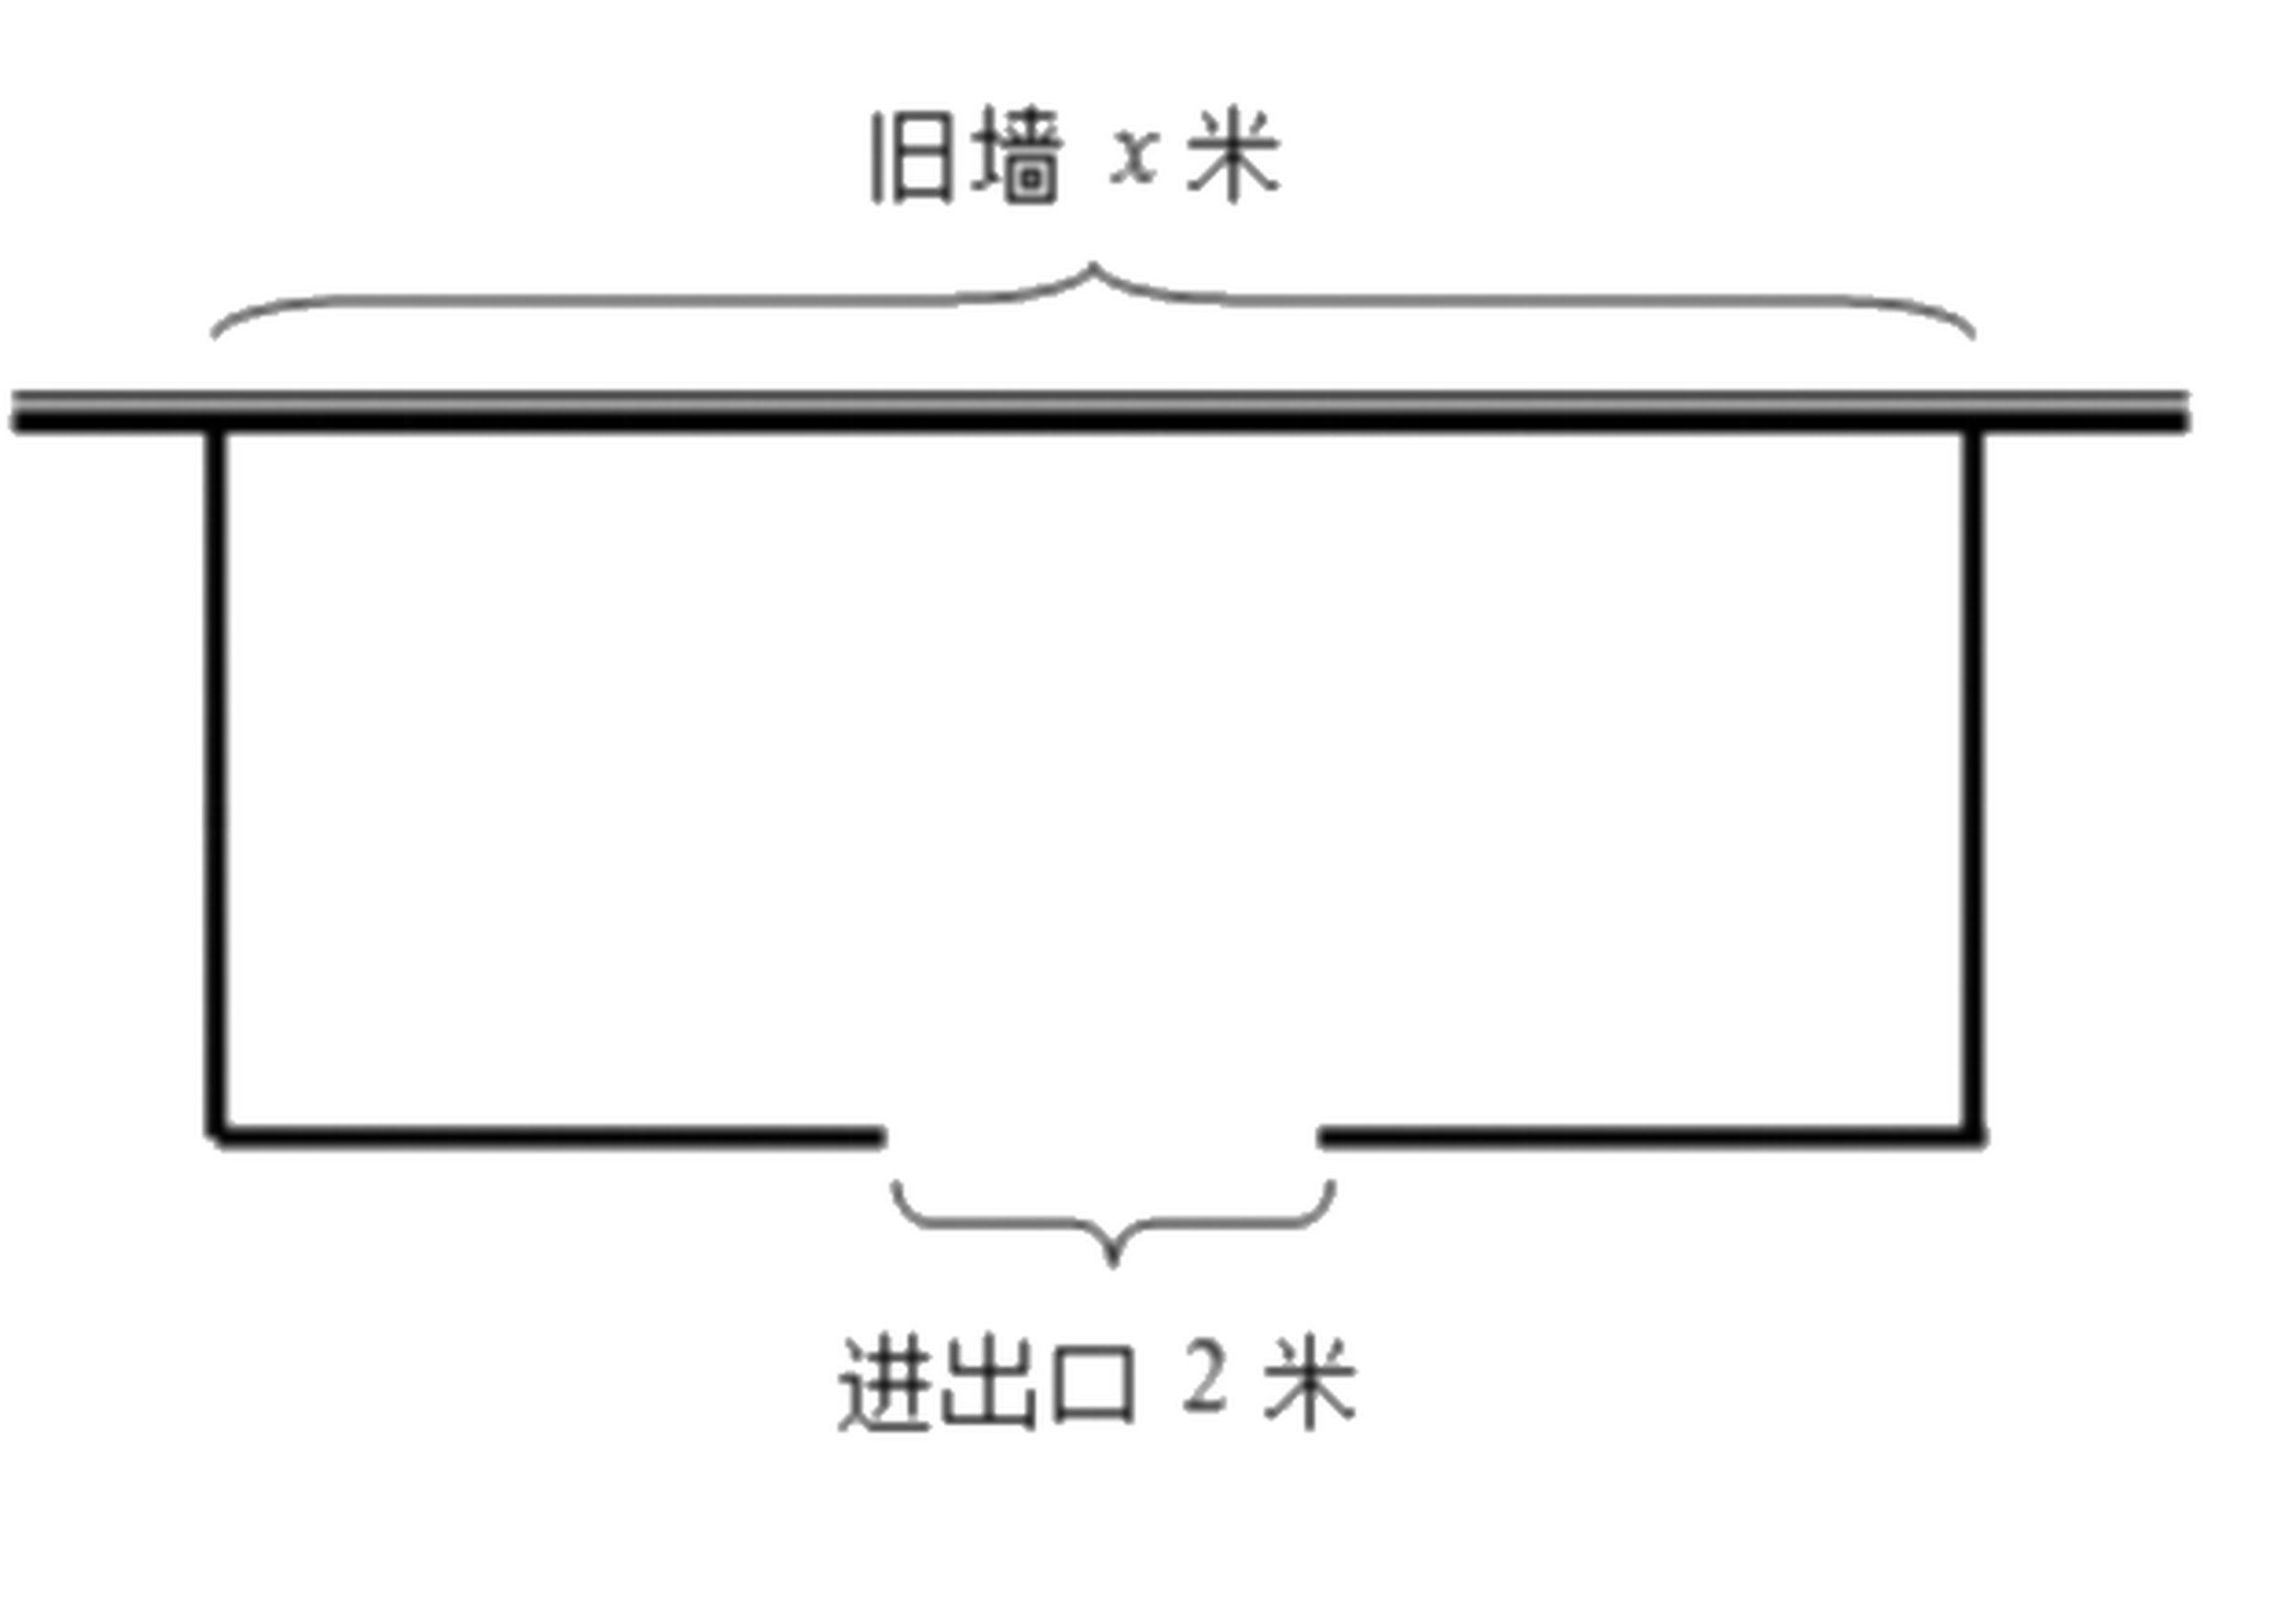
\includegraphics[width=0.60\textwidth]{figures/gao144_q17.png}
\end{center}

(1) 写出总费用 $y$ 关于 $x$ 的表达式;

(2) 试确定 $x$，使修建此矩形场地围墙的总费用最小，并求出最小总费用.

\ifanswer
\solbegin
\step{(1) 设矩形的另一边长为 $a$ 米，}
\step{则 $y=45x+180(x-2)+180\times2a=225x+360a-360$，}
\step{由已知 $xa=360$，得 $a=\dfrac{360}{x}$，所以 $y=225x+\dfrac{360^2}{x}-360(x>0)$;}
\step{(2) 因为 $x>0$，所以 $225x+\dfrac{360^2}{x}\geqslant2\sqrt{225x\cdot\dfrac{360^2}{x}}=10800$，}
\step{所以 $y=225x+\dfrac{360^2}{x}-360\geqslant10440$，}
\step{当且仅当 $225x=\dfrac{360^2}{x}$，即 $x=24$ 时取等号，}
\step{所以当 $x=24$ 米时，修建围墙的总费用最小，最小总费用是 10440 元.}
\solend
\fi

\item 已知集合 $A=\{a_1,a_2,\cdots,a_k\}(k\geqslant2)$，其中 $a_i\in\Z(i=1,2,\cdots,k)$. 定义：若对任意的 $x\in A$，必有 $-x\notin A$，则称集合 $A$ 具有性质 $G$. 由 $A$ 中元素可构成两个点集 $P$ 和 $Q$，$P=\{(x,y)\mid x\in A,y\in A,x+y\in A\}$，$Q=\{(x,y)\mid x\in A,y\in A,x-y\in A\}$，其中 $P$ 有 $m$ 个元素，$Q$ 中有 $n$ 个元素.

(1) 已知集合 $K=\{-1,2,3\}$，判断 $K$ 是否具有性质 $G$; 并写出 $K$ 对应的集合 $P$ 和集合 $Q$;

(2) 若集合 $A=\{1,2,3,4,5,6,7,8,9,10\}$，求对应集合 $Q$ 的元素个数; 一般地，若集合 $A$ 具有性质 $G$，且有 $k$ 个元素，猜测对应的集合 $Q$ 的元素最大个数，并说明理由;

(3) 若集合 $A$ 具有性质 $G$，猜测 $m,n$ 的大小并说明理由.

\ifanswer
\solbegin
\step{(1) 因为 $K=\{-1,2,3\},1,-2,-3$ 都不属于集合 $K$，}
\step{所以集合 $K$ 具有性质 $G$，}
\step{对应集合 $P=\{(-1,3),(3,-1)\},Q=\{(2,-1),(2,3)\}$;}
\step{(2) $A=\{1,2,3,4,5,6,7,8,9,10\}$，则对应集合 $Q$ 中的元素为:}
\step{$(2,1),(3,2),\cdots,(9,8),(10,9)$,}
\step{$(3,1),(4,2),\cdots,(9,7),(10,8)$,}
\step{$(4,1),(5,2),\cdots,(9,6),(10,7)$,}
\step{$\cdots$}
\step{$(9,1),(10,2)$,}
\step{$(10,1)$,}
\step{共有 $9+8+7+\cdots+2+1=45$ 个元素，即对应集合 $Q$ 的元素个数 45;}
\step{集合 $A$ 有 $k$ 个元素，猜测对应的集合 $Q$ 的最大个数为 $\dfrac{k^2-k}{2}$. 理由如下:}
\step{由题意得集合 $A$ 的元素构成有序数对 $(a_i,a_j)(i,j\in\N^*,i\leqslant k,j\leqslant k)$，}
\step{共有 $k^2$ 个，因为 $0\notin A$，所以 $(a_i,a_i)\notin Q$，}
\step{又因为 $a\in A$ 时，$-a\notin A$，所以 $(a_i,a_j)\in Q$ 时，$(a_j,a_i)\notin Q$，}
\step{所以集合 $Q$ 的元素个数为 $\dfrac{k^2-k}{2}$ 个，}
\step{(3) 当集合 $A$ 具有性质 $G$ 时，}
\step{①对于 $(a,b)\in P$，由定义得 $a\in A,b\in A,a+b\in A$，}
\step{又因为集合 $A$ 具有性质 $G$，所以 $(a+b,a)\in Q$，}
\step{如果 $(a,b),(c,d)$ 是 $P$ 中的不同元素，}
\step{那么 $a=c,b=d$ 中至少有一个不成立，}
\step{于是 $b=d,a+b=c+d$ 中至少有一个不成立，}
\step{故 $(a+b,b)$ 和 $(c+d,d)$ 也是 $Q$ 中不同的元素，}
\step{可见 $P$ 的元素个数不多于 $Q$ 的元素个数，即 $m\leqslant n$;}
\step{②对于 $(a,b)\in Q$，由定义得 $a\in A,b\in A,a-b\in A$，}
\step{又因为集合 $A$ 具有性质 $G$，则 $(a-b,b)\in P$，}
\step{如果 $(a,b),(c,d)$ 是 $Q$ 中的不同元素，}
\step{那么 $a=c,b=d$ 中至少有一个不成立，}
\step{于是 $b=d,a-b=c-d$ 中至少有一个不成立，}
\step{故 $(a-b,b)$ 和 $(c-d,d)$ 也是 $P$ 中不同的元素，}
\step{可见 $Q$ 的元素个数不多于 $P$ 的元素个数，即 $n\leqslant m$，}
\step{由①②得 $m=n$.}
\solend
\fi

\end{enumerate}

\end{document}
"
% 紧凑版：xelatex "\def\iscompact{1}% 高一144_风华中学_期中.tex
%   —— 高一上数学"2026-2027 年风华中学高一上期中"（试卷版/答案版/紧凑版）
% 试卷版：xelatex 高一144_风华中学_期中.tex
% 答案版：xelatex "\def\isanswer{1}% 高一144_风华中学_期中.tex
%   —— 高一上数学"2026-2027 年风华中学高一上期中"（试卷版/答案版/紧凑版）
% 试卷版：xelatex 高一144_风华中学_期中.tex
% 答案版：xelatex "\def\isanswer{1}% 高一144_风华中学_期中.tex
%   —— 高一上数学"2026-2027 年风华中学高一上期中"（试卷版/答案版/紧凑版）
% 试卷版：xelatex 高一144_风华中学_期中.tex
% 答案版：xelatex "\def\isanswer{1}\input{高一144_风华中学_期中.tex}"
% 紧凑版：xelatex "\def\iscompact{1}\input{高一144_风华中学_期中.tex}"
%
% ① 原始材料：微信公众号"魔都数学加油站"文章，连载"27学年高一144"，原文标题
% "27学年高一144——2026-2027年上海市风华中学高一上期中"；
% 原文链接：https://mp.weixin.qq.com/s/ylUlbXfudWOYC-jlH3jyjw 。
% 正文为 10 张 PNG 页，题目下印【解析】，为讲评版。
% 各页分辨率：01/02/03/05/06/07/09/10 为 2560×3620，04/08 为 4762×6735。
% 题目、解析均据原图转录；卷面粉红色水印"魔都数学加油站"及公众号页脚未录入。
% 全卷插图情况：Q17 有一幅矩形场地示意图（旧墙 x 米 / 进出口 2 米），从 07 页裁出、
%   去粉色水印去色 4× LANCZOS 放大存 figures/gao144_q17.png；其余 9 页逐页通读
%   确认无题目配图、无表格、亦无"题干写如图而源码漏图"一处。
%
% 卷首标题：原卷印作"2026-2027 年风华中学高一上期中"，年份区间按全稿惯例排 en dash；
% 原卷卷面未印副标题，本稿按同期中卷（高一140／141／143）知识模块口径补出
% "集合与常用逻辑用语、不等式、函数"：集合与逻辑见 Q3、Q7、Q9、Q10、Q12、Q16、Q18，
% 不等式见 Q6、Q11、Q13、Q14、Q15、Q17，函数见 Q4、Q5、Q8、Q9。
%
% 题号体例：本卷共 16 题——一、填空题 3—10（8 题）、二、选择题 11—13（3 题）、
% 三、解答题 14—18（5 题）。三节分别 \setcounter{enumi}{2}／{10}／{13}。
% 原卷从第 3 题起、无第 1、2 题，本稿保留原题号；全卷无附加题节。
%
% ② 与原卷的排版差异：
%   ① 原文从第 3 题起，本稿保留原题号；共 16 题三节；
%   ② 原卷 15 题题下印【解析】，唯 Q11 未印【解析】、只把答案"（ BD ）"直接印在
%      题干括号内（放大 04 页 A/B 选项与 05 页 C/D 选项衔接处确认，见 ⑤）；
%      按 高一128／94／106／140 成例：Q11 试卷版括号留空 \mbox{（\quad）}、
%      答案版另提 \ans{$BD$}、不补造原卷没有的解析；其余 15 题印【解析】、
%      括号内一律留空、不另提 \ans{}（Q12 选 C、Q13 选 B 在解析末句"故选 …"）；
%      答案版【答案】/【解析】标记数 = 16（1 个 \ans + 15 个 \solbegin）= 全卷题数；
%      正文 Q11 对应处另有 % 注；
%   ③ 原卷卷面未印副标题，本稿按知识模块口径补出；
%   ④ 原卷填空横线按全稿惯例排 \blankline[4.4em]；选择题括号排 \mbox{（\quad）}，
%      选项段前按惯例加 \keepwithprev；解答题不留作答区、不加 \anspace
%      （原卷为讲评版，与 129／131／132／133／136／140／141／143 同）；
%   ⑤ 数集：Q9 题干与解析"a,b∈R"、Q12 题干"U=R"、Q15 题干"x,y∈R"原卷印
%      斜体或黑板粗体 R，Q18 题干"a_i∈Z"印黑板粗体 Z、Q18 解析"i,j∈N*"印
%      黑板粗体 N，按全稿惯例统一改 \R／\Z／\N^*；绝对值排 \lvert…\rvert，
%      集合描述竖线排 \mid；不等号按全稿惯例排 \leqslant／\geqslant；
%      补集照原卷上划线排 \overline{A}／\overline{B}；空集记号 \varnothing；
%   ⑥ 子题标号 (1)(2)(3) 原卷印半角括号，照录；圈数字 ①② 在正文（文本模式）
%      按原卷照录（Q15、Q18 解析），未进数学式；数学式内半角逗号照录
%      （Q12 解析"$A=(1,2),B=(0,6)$"、Q18 解析"$(a_i,a_j)(i,j\in\N^*,i\leqslant k,j\leqslant k)$"、
%      Q15 解析"$x=1,y=-1$"、Q18 解析"$a=c,b=d$"等，为全稿惯例、非笔误）；
%      全卷行末西文句点照录为 ASCII `.`；行中全角逗号／顿号照录；
%      Q18 解析集合描述中的"或"用 \text{ 或 } 置于数学式内；
%   ⑦ 题干中的中文弯引号按原卷照录（Q3 的" x∈A "／" x∈B "与 Q15 (2) 的命题
%      引号，含引号内空格），注释内一律 ASCII 引号；
%   ⑧ Q17 配图：题干写"如图所示"，配图居中排在题干之后、子问之前，三版都出；
%      在 Q17 \item 之前加 \needvspace{10cm} 把"题干＋图"整块推走。Q17 是
%      "三、解答题"节内第 4 题（非节首题），故守卫放在 \item 之前而非 \bigsec
%      之前不会让节标题孤落页末（B 类）；三版切页审计均"合计异常：无"；
%   ⑨ 跨页续印按题合并：Q3 在 01 页；Q4/5/6 在 01 页（Q6 解析续到 02 页顶）；
%      Q7/8/9 在 02 页（Q9 题干跨 02→03）；Q10 在 03 页、解析跨 03→04（很长，
%      按余数分组 A₁/A₂/A₃）；Q11 在 04 页（"二、选择题"节标题也在 04 页下部）、
%      Q12/13 在 05 页（"三、解答题"标题在 05 页下部）；Q14 在 05 页末、解析在 06 页；
%      Q15/16 在 06 页（Q16 续到 07 页）；Q17 在 07 页；Q18 在 08 页、解析跨
%      08/09/10 页（性质 G 压轴，3 问，很长）；本稿按题连排，不丢行、不并折行；
%   ⑩ Q8 解析"法一：""法二："两处标签经放大 02 页逐字确认原卷均印红色
%      （见 ⑤）；按全稿惯例（高一53 成例）不引入红色、均照录为黑体着色
%      \stepm{法一：}{…}／\stepm{法二：}{…}，不改 common.sty；
%      文件头在此注明原卷为红色；
%   ⑪ "图像／图象"逐处核：全卷未出现"图像"或"图象"字样，无统一问题；
%   ⑫ \left…\right 不得拆到不同 $…$ 组；cases 块整体算一个印刷行；
%      Q4 分式与 8×(-3/4) 同一 $…$ 组，Q13 的 \left(\frac1x+\frac2y\right) 同理。
%
% ③ 行数复核：一条 \step／\stepm 行 = 原卷解析的一个印刷行，cases 块作一个印刷行计。
%   逐题数（含 \stepm）：Q3：3；Q4：1；Q5：1；Q6：5；Q7：4；Q8：8（6 \step
%   ＋ 2 \stepm，法一/法二标签各占 1 行）；Q9：6；Q10：23；Q11：0（原卷无解析，
%   答案另提 \ans{$BD$}）；Q12：5；Q13：3；Q14：5；Q15：8；Q16：7；Q17：7；
%   Q18：32。合计 116 条 \step ＋ 2 条 \stepm ＝ 118 个印刷行，与原卷逐题相等。
%   全卷 15 题设 \solbegin…\solend ＋ Q11 一处 \ans{}，答案版【答案】/【解析】
%   标记数 = 16 = 全卷题数。
%
% ④ 判别式／子集符号结论（逐处放大原图照录、不得统一）：
%   判别式全卷 2 处，逐页放大扫过 10 页确认（Q4 为分式指数化简、不含判别式）：
%     · Q9【解析】"所以 △=a^2-4b=0" 原卷印细线、扁等边三角（宽≈高、笔画细，
%       放大见 /tmp/gao144fh/z_q9_tri.png、z_tri_Q9.png），照录 \triangle；
%     · Q15 (2)【解析】cases 块"Δ=(a-2)^2-4(a-2)≤0" 原卷印等腰偏高、粗笔画
%       三角（高>宽，放大见 z_q15_tri.png、z_tri_Q15.png），照录 \Delta；
%   两形不同、全卷混用，逐处照录不统一（参照 高一142 头注④口径）。
%   子集符号全卷 4 处，逐处放大核：
%     · Q3 解析"所以 B⊆A"、Q16 (1) 解析"所以 B⊆A" 原卷均印带下划线的 ⊆
%       （z_q3_symbol.png、z_q16_subset2.png），照录 \subseteq；
%     · Q12 选项 B"$\overline{A}\subset B$" 原卷印单线 ⊂（z_q12_opts2.png），
%       照录 \subset；Q12 解析"$\overline{A}=(-\infty,1]\cup[2,+\infty)\not\subset B$"
%       原卷印单线带斜杠 ⊄（z_q12_notsym3.png），照录 \not\subset；
%   \subset 与 \subseteq 混用，逐处照录不统一。补集照原卷上划线 \overline{A}／
%   \overline{B}，空集 \varnothing，数集 \R／\Z／\N^* 归一见 ② ⑤。
%
% ⑤ 存疑／特殊体例（主会话逐处放大原图复核确认，照录未改，正文对应处另有 % 注）：
%   1. 第 11 题原卷把答案"（ BD ）"直接印在题干括号内、题下未印【解析】
%      （放大 04 页 A/B 选项与 05 页 C/D 选项衔接处确认：05 页顶 C/D 选项后
%      直接接第 12 题）。按 高一128／94／106／140 成例括号留空、另提
%      \ans{$BD$}，不补造解析（不编造）。
%   2. 第 10 题题干"集合 $S$ 为集合 $M=\{1,2,3,4,\cdots,2026\}$，的子集"在
%      集括号与"的子集"之间原卷多印一个全角逗号（放大 03 页确认），
%      按存疑照录未删，正文对应处另有 % 注。
%   3. 第 8 题解析"法一：""法二："两处原卷均印红色（放大 02 页逐字确认），
%      按全稿惯例不引入红色、两处均照录为黑体着色 \stepm（见 ② ⑩）。
%   全卷除此 3 条外未发现其它笔误／自相矛盾处。
%
% ⑥ 跨页续印按题合并说明：见 ② ⑨。
%
\documentclass[a4paper,11pt]{article}
\usepackage{common}

\begin{document}

\examtitlest[3]{2026--2027 年风华中学高一上期中}{集合与常用逻辑用语、不等式、函数}

\bigsec{一、填空题}

\begin{enumerate}
\setcounter{enumi}{2}

\item $A=\{x\mid x>4\}$，$B=\{x\mid x>a\}$，若命题 “ $x\in A$ ” 是命题 “ $x\in B$ ” 的必要条件，则 $a$ 的取值范围是\blankline[4.4em].

\ifanswer
\solbegin
\step{因为 “ $x\in A$ ” 是命题 “ $x\in B$ ” 的必要条件，所以 $B\subseteq A$，}% 子集符号原卷印带下划线 $\subseteq$，照录
\step{因为 $A=\{x\mid x>4\}$，$B=\{x\mid x>a\}$，所以 $a\geqslant4$，}
\step{所以 $a$ 的取值范围是 $\{a\mid a\geqslant4\}$.}
\solend
\fi

\item 已知 $a>0,b>0$，化简式子：$\dfrac{8a^{\frac34}b^3}{\left(a^{\frac16}b^{\frac32}\right)\left(-\dfrac43 a^{\frac1{12}}b^{\frac12}\right)}=$\blankline[4.4em].

\ifanswer
\solbegin
\step{$\dfrac{8a^{\frac34}b^3}{\left(a^{\frac16}b^{\frac32}\right)\left(-\dfrac43 a^{\frac1{12}}b^{\frac12}\right)}=8\times\left(-\dfrac34\right)a^{\frac34-\frac16-\frac1{12}}b^{3-\frac32-\frac12}=-6a^{\frac12}b=-6b\sqrt a$.}
\solend
\fi

\item 已知 $\lg2=a$，$\lg3=b$，则 $\log_5 6=$\blankline[4.4em]（结果用 $a,b$ 表示）.

\ifanswer
\solbegin
\step{$\log_5 6=\dfrac{\lg6}{\lg5}=\dfrac{\lg2+\lg3}{1-\lg2}=\dfrac{a+b}{1-a}$.}
\solend
\fi

\item 若关于 $x$ 的不等式 $ax>b$ 的解集为 $(-\infty,2)$，则不等式 $bx+a>0$ 的解集为\blankline[4.4em].

\ifanswer
\solbegin
\step{因为不等式 $ax>b$ 的解集为 $(-\infty,2)$，所以 $a<0$，}
\step{所以由不等式解得 $x<\dfrac ba$，所以 $\dfrac ba=2$，即 $b=2a$，}
\step{代入不等式 $bx+a>0$，得 $2ax+a>0$，}
\step{因为 $a<0$，所以不等式化为 $2x+1<0$，解得 $x<-\dfrac12$，}
\step{故不等式的解集为 $\left(-\infty,-\dfrac12\right)$.}
\solend
\fi

\item 如果集合 $A=\{x\mid x^2-4x\leqslant0\}$，$B=\{x\mid x^2+ax+b\leqslant0\}$，$A\cap B=\{x\mid3\leqslant x\leqslant4\}$，$A\cup B=\{x\mid0\leqslant x\leqslant5\}$，则 $a+b=$\blankline[4.4em].

\ifanswer
\solbegin
\step{由题意得 $A=\{x\mid x^2-4x\leqslant0\}=[0,4]$，}
\step{又因为 $A\cap B=\{x\mid3\leqslant x\leqslant4\}$，$A\cup B=\{x\mid0\leqslant x\leqslant5\}$，}
\step{所以 $B=\{x\mid3\leqslant x\leqslant5\}$，即方程 $x^2+ax+b=0$ 的两根为 $3,5$，}
\step{由韦达定理得 $\begin{cases}3+5=-a\\3\times5=b\end{cases}$，解得 $a=-8$，$b=15$，所以 $a+b=15-8=7$.}
\solend
\fi

% 第 8 题：原卷"法一：""法二："两处标签均印红色（8× 放大确认）；按交办口径
% "法一"用普通 \step、"法二："排 \stepm（加粗着色、不引红色），见头注 ② ⑩／⑤
\item 若关于 $x$ 的方程 $\lvert x-1\rvert+\lvert\pi-x\rvert=\pi-1$ 的解集为\blankline[4.4em].

\ifanswer
\solbegin
\stepm{法一：}{因为 $\lvert x-1\rvert+\lvert\pi-x\rvert=\begin{cases}x-1+x-\pi,x\geqslant\pi\\\pi-1,1<x<\pi\\1-x+\pi-x,x\leqslant1\end{cases}=\begin{cases}2x-1-\pi,x\geqslant\pi\\\pi-1,1<x<\pi\\1+\pi-2x,x\leqslant1\end{cases}$.}
\step{当 $x\geqslant\pi$ 时，令 $2x-1-\pi=\pi-1$，得 $x=\pi$；}
\step{当 $1<x<\pi$ 时，$\lvert x-1\rvert+\lvert\pi-x\rvert=\pi-1$ 恒成立；}
\step{当 $x\leqslant1$ 时，令 $1+\pi-2x=\pi-1$，得 $x=1$.}
\step{综上所述，方程 $\lvert x-1\rvert+\lvert\pi-x\rvert=\pi-1$ 的解集为 $[1,\pi]$.}
\stepm{法二：}{因为 $\lvert x-1\rvert+\lvert\pi-x\rvert\geqslant\lvert x-1+\pi-x\rvert=\pi-1$，}
\step{当且仅当 $(x-1)(\pi-x)\geqslant0$ 时取等号，}
\step{故方程 $\lvert x-1\rvert+\lvert\pi-x\rvert=\pi-1$ 的解集为 $[1,\pi]$.}
\solend
\fi

% 第 9 题：题干跨 02→03 页；解析判别式原卷印细线扁等边三角 $\triangle$，照录
\item 已知函数 $f(x)=x^2+ax+b(a,b\in\R)$ 和 $x$ 轴有且只有一个交点，若关于 $x$ 的不等式 $f(x)<c$ 的解集为 $(m,m+6)$，则 $c=$\blankline[4.4em].

\ifanswer
\solbegin
\step{因为函数 $f(x)=x^2+ax+b(a,b\in\R)$ 和 $x$ 轴有且只有一个交点，}
\step{所以 $\triangle=a^2-4b=0$，即 $b=\dfrac{a^2}{4}$，}% 判别式原卷印扁等边三角 $\triangle$，照录
\step{不等式 $f(x)<c$ 的解集为 $(m,m+6)$，}
\step{即 $x^2+ax+\dfrac{a^2}{4}-c<0$ 的解集为 $(m,m+6)$，}
\step{所以方程 $x^2+ax+\dfrac{a^2}{4}-c=0$ 的两个根为 $x_1=m$，$x_2=m+6$，}
\step{所以 $\begin{cases}x_1+x_2=2m+6=-a\\x_1x_2=m(m+6)=\dfrac{a^2}{4}-c\end{cases}$，消去 $m$ 得 $\dfrac{a^2}{4}-9=\dfrac{a^2}{4}-c$，解得 $c=9$.}
\solend
\fi

% 第 10 题：原卷题干在集括号与"的子集"之间多印一个全角逗号，照录未改（存疑，见头注 ⑤）
\item 已知集合 $S$ 为集合 $M=\{1,2,3,4,\cdots,2026\}$，的子集，并且集合 $S$ 中任意两个元素之和不能被 3 整除，则集合 $S$ 中元素个数的最大值为\blankline[4.4em].

\ifanswer
\solbegin
\step{对于集合 $M=\{1,2,3,4,\cdots,2026\}$，}
\step{所有被 3 除余数为 0 的元素组成的集合为 $A_3=\{3,6,9,\cdots,2025\}$，}
\step{元素个数为 675;}
\step{所有被 3 除余数为 1 的元素组成的集合为 $A_1=\{1,4,7,\cdots,2026\}$，}
\step{元素个数为 676;}
\step{所有被 3 除余数为 2 的元素组成的集合为 $A_2=\{2,5,8,\cdots,2024\}$，}
\step{元素个数为 675;}
\step{集合 $S$ 中任意两个元素之和不能被 3 整除，}
\step{若两个元素分别来自 $A_1$ 和 $A_2$，则两数之和除以 3 的余数为 $1+2=3\equiv0$，}
\step{即和能被 3 整除，}
\step{所以 $S$ 不能同时包含 $A_1$ 和 $A_2$ 中的元素，}
\step{即 $S$ 最多只能选取 $A_1$、$A_2$ 一个集合中的全部元素;}
\step{若两个元素都来自 $A_3$，则两数之和除以 3 的余数为 $0+0=0$，即和能被 3 整除，}
\step{所以 $S$ 中最多包含 $A_3$ 中的 1 个元素;}
\step{对 $A_1$ 内的任意两个元素，其和除以 3 的余数为 $1+1=2$，不能被 3 整除;}
\step{$A_1$ 中元素与 $A_3$ 中元素的和除以 3 余数为 $1+0=1$，不能被 3 整除，}
\step{所以 $A_1$ 的全部元素与 $A_3$ 中的任意 1 个元素的组合满足题意;}
\step{对 $A_2$ 内的任意两个元素，其和除以 3 的余数为 $2+2=4\equiv1$，不能被 3 整除;}
\step{$A_2$ 中元素与 $A_3$ 中元素的和除以 3 的余数为 $2+0=2$，不能被 3 整除，}
\step{所以 $A_2$ 的全部元素与 $A_3$ 中任意 1 个元素的组合也满足题意.}
\step{故若选取 $A_2$ 全部元素加 1 个 $A_3$ 元素，总个数为 $675+1=676$;}
\step{选取 $A_1$ 全部元素加 1 个 $A_3$ 元素，总个数为 $676+1=677$;}
\step{所以集合 $S$ 中元素个数的最大值为 677.}
\solend
\fi

\end{enumerate}

\bigsec{二、选择题}

\begin{enumerate}
\setcounter{enumi}{10}

% 第 11 题：原卷把答案"（ BD ）"直接印在题干括号内、题下无【解析】（放大 04 页 A/B 选项
% 与 05 页 C/D 选项衔接处确认）。按 高一128／94／106／140 成例：试卷版括号留空、
% 答案版另提 \ans{$BD$}、不补造原卷没有的解析（不编造）。
\item 已知实数 $a,b$，下列四个不等式中正确的是\mbox{（\quad）}

\keepwithprev
A. $a+\dfrac1a\geqslant2$\qquad B. $\sqrt{a^2+2}+\dfrac{1}{\sqrt{a^2+2}}\geqslant2$

C. $\dfrac{a+b}{2}\leqslant\sqrt{ab}$\qquad D. $a^2+b^2\geqslant2ab$

\ifanswer
\ans{$BD$}
\fi

\item 若全集 $U=\R$，$A=\{x\mid x^2-3x+2<0\}$，$B=\{x\mid0<x<6\}$，则\mbox{（\quad）}

\keepwithprev
A. $A\cap B=B$\qquad B. $\overline{A}\subset B$\qquad C. $A\cap\overline{B}=\varnothing$\qquad D. $A\cup B=A$

\ifanswer
\solbegin
\step{由 $x^2-3x+2<0$，则 $A=(1,2),B=(0,6)$，所以 $A\cap B=(1,2)=A,A$ 错误;}
\step{$\overline{A}=(-\infty,1]\cup[2,+\infty)\not\subset B$，$B$ 错误;}
\step{$\overline{B}=(-\infty,0]\cup[6,+\infty)$，所以 $A\cap\overline{B}=\varnothing,C$ 正确;}
\step{$A\cup B=(0,6)\ne A,D$ 错误.}
\step{故选 $C$.}
\solend
\fi

\item 已知正数 $x$、$y$ 满足 $\dfrac1x+\dfrac2y=1$，不等式 $3x+2y-1>m$ 恒成立，则实数 $m$ 的取值范围是\mbox{（\quad）}

\keepwithprev
A. $(-\infty,4+6\sqrt2)$\qquad B. $(-\infty,6+4\sqrt3)$\qquad C. $(6+4\sqrt2,+\infty)$\qquad D. $(8+4\sqrt3,+\infty)$

\ifanswer
\solbegin
\step{$3x+2y=(3x+2y)\left(\dfrac1x+\dfrac2y\right)=7+\dfrac{6x}{y}+\dfrac{2y}{x}\geqslant7+2\sqrt{\dfrac{6x}{y}\cdot\dfrac{2y}{x}}=7+4\sqrt3$，}
\step{当且仅当 $\dfrac{6x}{y}=\dfrac{2y}{x}$，即 $y=\sqrt3x=\sqrt3+2$ 时取等号，}
\step{故要使原式成立，只需 $m<6+4\sqrt3$. 故选 $B$.}
\solend
\fi

\end{enumerate}

\bigsec{三、解答题}

\begin{enumerate}
\setcounter{enumi}{13}

\item 解关于 $x$ 的不等式：

(1) $x^2-2\lvert x\rvert-3>0$；

(2) $\dfrac{2x-1}{x+2}<1$.

\ifanswer
\solbegin
\step{(1) 原不等式等价于 $(\lvert x\rvert-3)(\lvert x\rvert+1)>0$，}
\step{$\lvert x\rvert+1>0$，故 $\lvert x\rvert>3$，解得 $x<-3$ 或 $x>3$，}
\step{故不等式的解集为 $(-\infty,-3)\cup(3,+\infty)$.}
\step{(2) 已知 $\dfrac{2x-1}{x+2}<1$，则 $\dfrac{2x-1}{x+2}-1<0$，即 $\dfrac{x-3}{x+2}<0$，}
\step{等价于 $(x-3)(x+2)<0$，解得 $-2<x<3$，故不等式的解集为 $(-2,3)$.}
\solend
\fi

\item (1) 已知 $x,y\in\R$，比较 $x^2+y^2$ 与 $2x-2y-2$ 的大小.

(2) “不等式 $(a-2)x^2+(a-2)x+1\geqslant0$ 对一切实数恒成立” 是假命题，求实数 $a$ 的取值范围.

\ifanswer
\solbegin
\step{(1) $x^2+y^2-(2x-2y-2)=x^2+y^2-2x+2y+2=(x-1)^2+(y+1)^2\geqslant0$，}
\step{故 $x^2+y^2\geqslant2x-2y-2$，当且仅当 $x=1,y=-1$ 时取等号.}
\step{(2) 先求命题 “$(a-2)x^2+(a-2)x+1\geqslant0$ 对一切实数恒成立” 为真，}
\step{①当 $a-2=0$ 时，即 $a=2$，不等式化为 $1\geqslant0$，成立，符合条件，}
\step{②当 $a-2\ne0$ 时，则 $\begin{cases}a-2>0\\\Delta=(a-2)^2-4(a-2)\leqslant0\end{cases}$，解得 $2<a\leqslant6$，}% 判别式原卷印等腰偏高三角 $\Delta$，照录
\step{综上①②，命题为真时 $2\leqslant a\leqslant6$，}
\step{该命题为假命题，则 $a<2$ 或 $a>6$，}
\step{所以实数 $a$ 的取值范围是 $(-\infty,2)\cup(6,+\infty)$.}
\solend
\fi

\item 设集合 $A=\{x\mid-1\leqslant x\leqslant2\}$，$B=\{x\mid m-1<x<2m+1\}$.

(1) 若 $A\cup B=A$，求实数 $m$ 的取值范围;

(2) 若 $B\cap\overline{A}$ 中只有一个整数 $-2$，求实数 $m$ 的取值范围.

\ifanswer
\solbegin
\step{(1) 因为 $A\cup B=A$，所以 $B\subseteq A$，}% 子集符号原卷印带下划线 $\subseteq$，照录
\step{当 $B=\varnothing$ 时，有 $m-1\geqslant2m+1$，解得 $m\leqslant-2$；}
\step{当 $B\ne\varnothing$ 时，有 $\begin{cases}m-1<2m+1\\m-1\geqslant-1\\2m+1\leqslant2\end{cases}$，解得 $0\leqslant m\leqslant\dfrac12$，}
\step{所以实数 $m$ 的取值范围是 $(-\infty,-2]\cup\left[0,\dfrac12\right]$;}
\step{(2) 由集合 $A=\{x\mid-1\leqslant x\leqslant2\}$，得 $\overline{A}=\{x\mid x<-1\text{ 或 }x>2\}$，}
\step{若 $B\cap\overline{A}$ 中只有一个整数 $-2$，则 $B\ne\varnothing$，且满足 $\begin{cases}m-1<2m+1\\-3\leqslant m-1<-2\\-2<2m+1\leqslant3\end{cases}$}
\step{解得 $-\dfrac32<m<-1$，所以实数 $m$ 的取值范围是 $\left(-\dfrac32,-1\right)$.}
\solend
\fi

% 第 17 题配图是"题干＋图"整块；守卫放在 \item 之前（Q17 非节首题，不会让节标题孤落页末）
\needvspace{10cm}
\item 现要围建一个面积为 360 平方米的矩形场地，要求矩形场地的一面利用旧墙（利用旧墙需维修），其它三面围墙要新建，在旧墙的对面的新墙上要留一个宽度为 2 米的进出口，如图所示，已知旧墙的维修费用为 45 元/米，新墙的造价为 180 元/米，设利用的旧墙的长度为 $x$ 米，工程总造价为 $y$（单位：元）.

\begin{center}
% 矩形场地示意图取自 07 页右侧，去粉色水印、去色、4× LANCZOS 放大
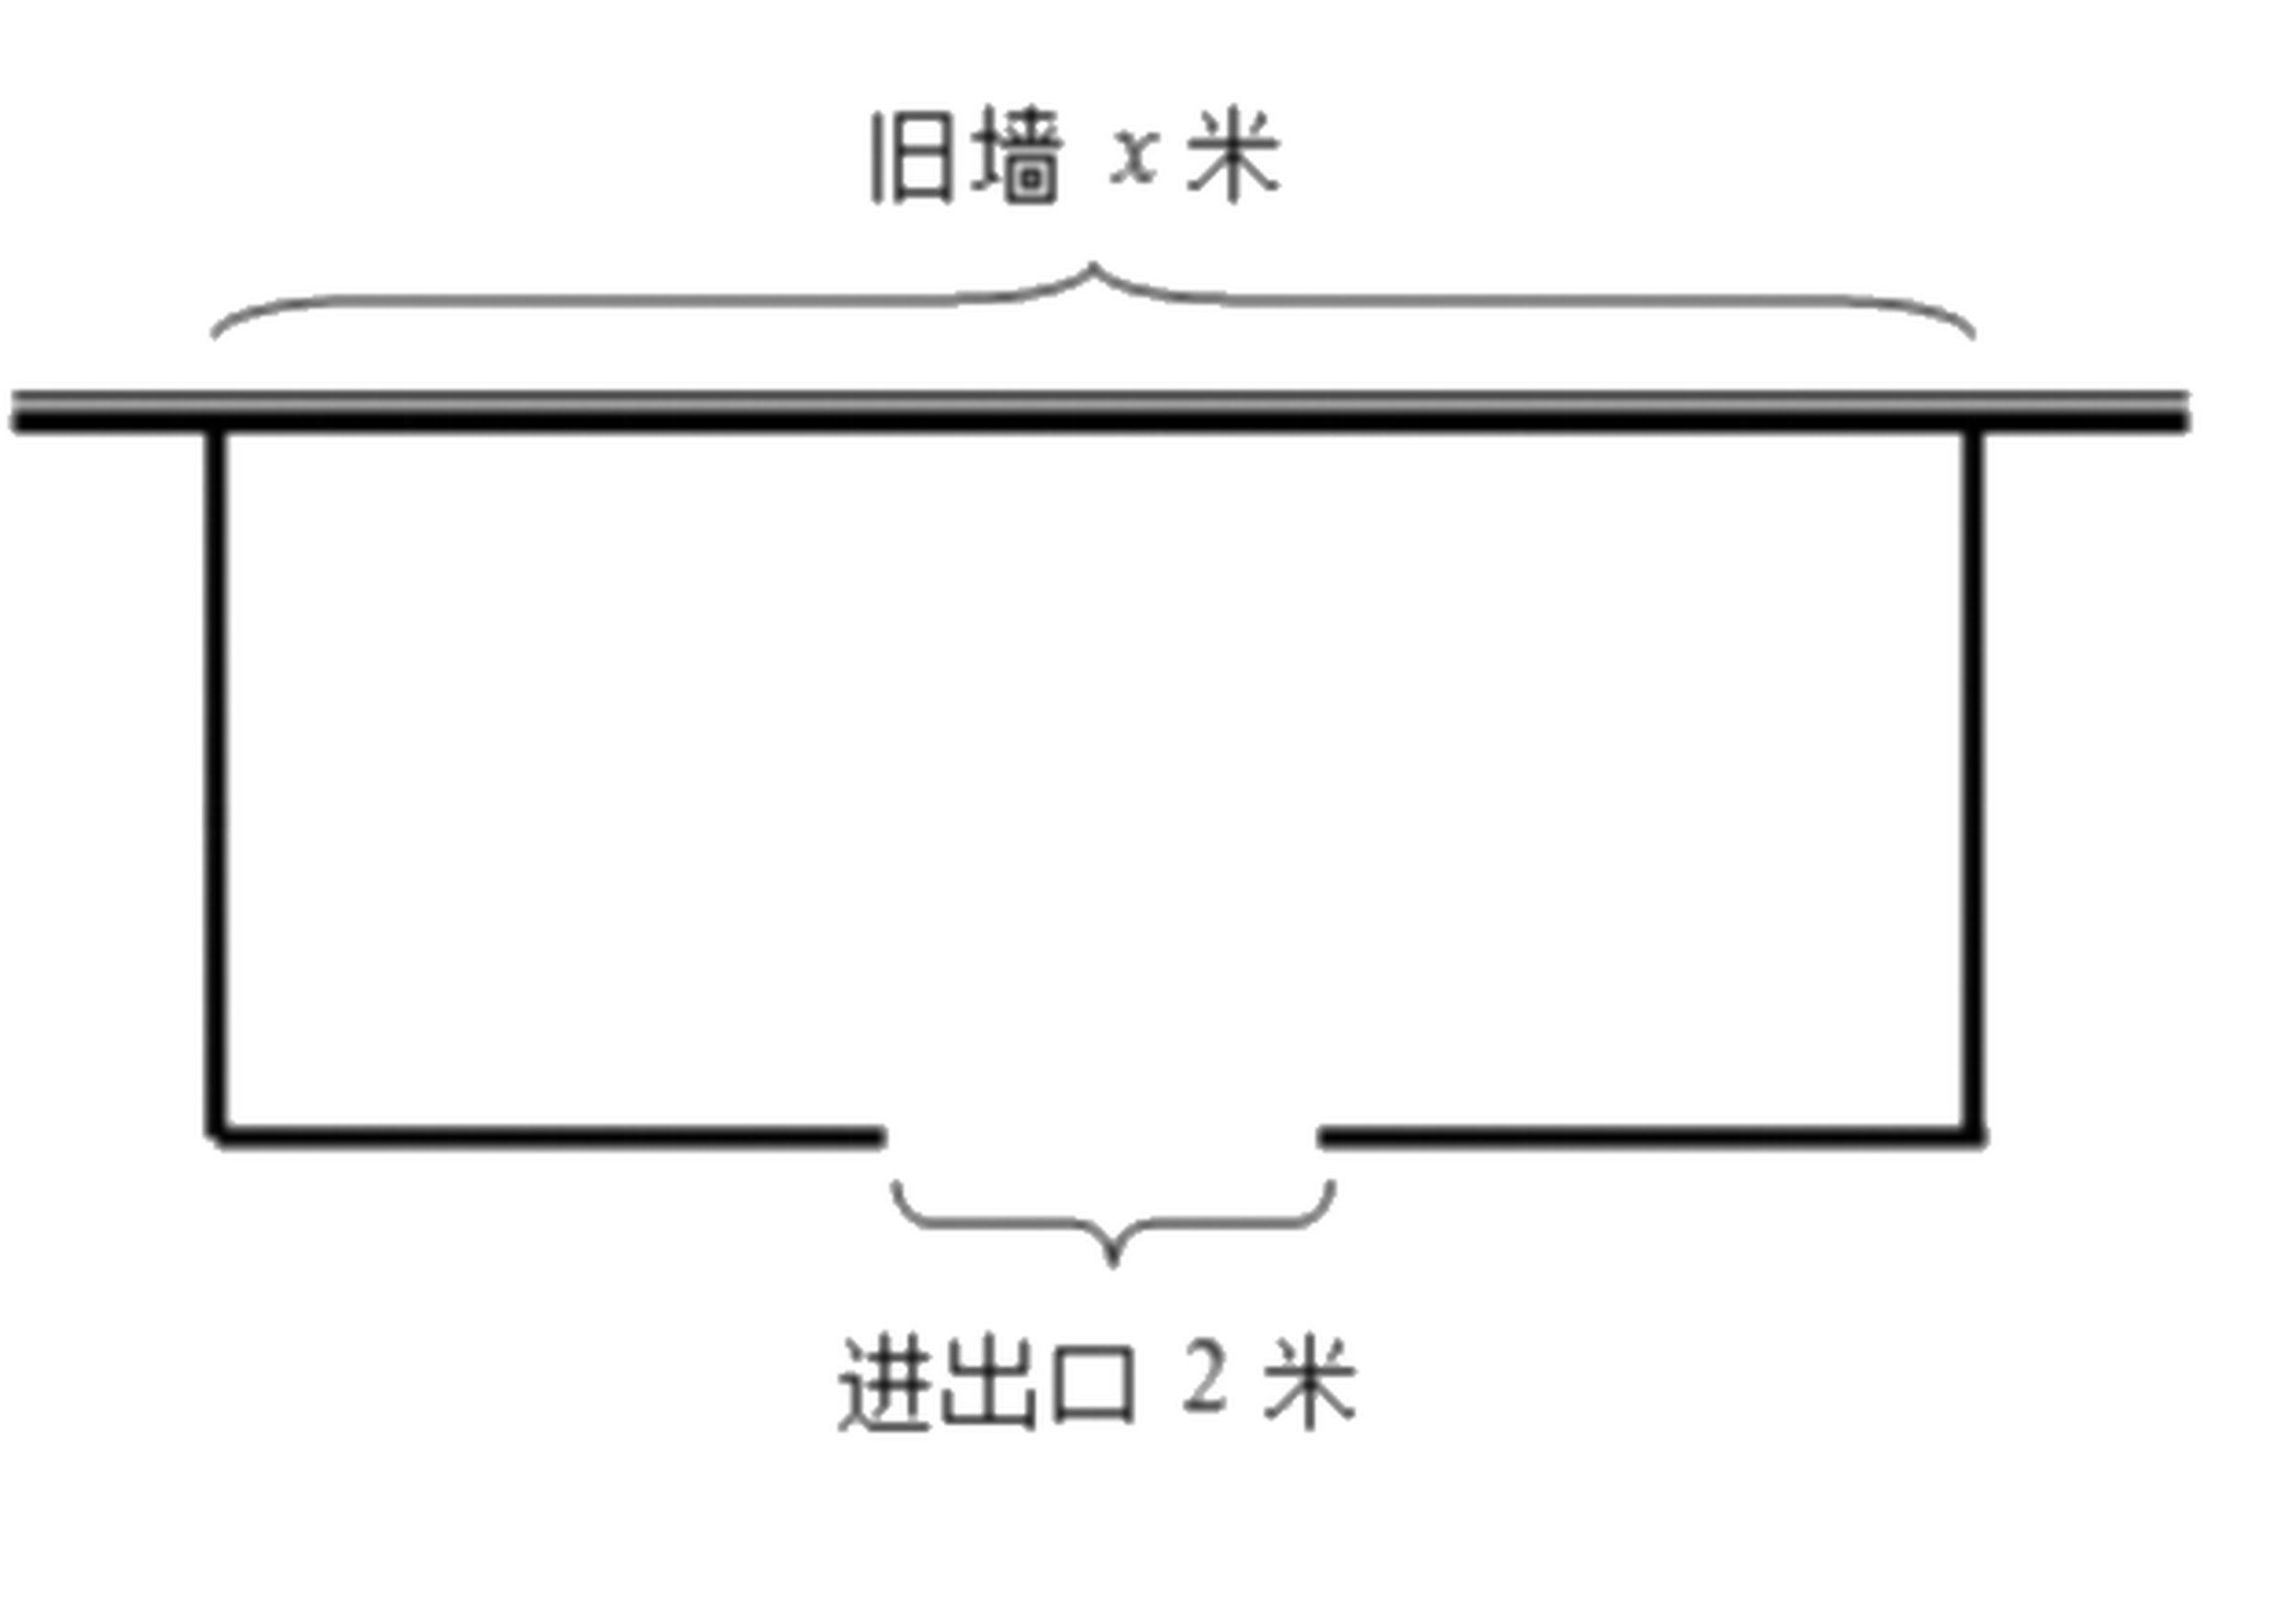
\includegraphics[width=0.60\textwidth]{figures/gao144_q17.png}
\end{center}

(1) 写出总费用 $y$ 关于 $x$ 的表达式;

(2) 试确定 $x$，使修建此矩形场地围墙的总费用最小，并求出最小总费用.

\ifanswer
\solbegin
\step{(1) 设矩形的另一边长为 $a$ 米，}
\step{则 $y=45x+180(x-2)+180\times2a=225x+360a-360$，}
\step{由已知 $xa=360$，得 $a=\dfrac{360}{x}$，所以 $y=225x+\dfrac{360^2}{x}-360(x>0)$;}
\step{(2) 因为 $x>0$，所以 $225x+\dfrac{360^2}{x}\geqslant2\sqrt{225x\cdot\dfrac{360^2}{x}}=10800$，}
\step{所以 $y=225x+\dfrac{360^2}{x}-360\geqslant10440$，}
\step{当且仅当 $225x=\dfrac{360^2}{x}$，即 $x=24$ 时取等号，}
\step{所以当 $x=24$ 米时，修建围墙的总费用最小，最小总费用是 10440 元.}
\solend
\fi

\item 已知集合 $A=\{a_1,a_2,\cdots,a_k\}(k\geqslant2)$，其中 $a_i\in\Z(i=1,2,\cdots,k)$. 定义：若对任意的 $x\in A$，必有 $-x\notin A$，则称集合 $A$ 具有性质 $G$. 由 $A$ 中元素可构成两个点集 $P$ 和 $Q$，$P=\{(x,y)\mid x\in A,y\in A,x+y\in A\}$，$Q=\{(x,y)\mid x\in A,y\in A,x-y\in A\}$，其中 $P$ 有 $m$ 个元素，$Q$ 中有 $n$ 个元素.

(1) 已知集合 $K=\{-1,2,3\}$，判断 $K$ 是否具有性质 $G$; 并写出 $K$ 对应的集合 $P$ 和集合 $Q$;

(2) 若集合 $A=\{1,2,3,4,5,6,7,8,9,10\}$，求对应集合 $Q$ 的元素个数; 一般地，若集合 $A$ 具有性质 $G$，且有 $k$ 个元素，猜测对应的集合 $Q$ 的元素最大个数，并说明理由;

(3) 若集合 $A$ 具有性质 $G$，猜测 $m,n$ 的大小并说明理由.

\ifanswer
\solbegin
\step{(1) 因为 $K=\{-1,2,3\},1,-2,-3$ 都不属于集合 $K$，}
\step{所以集合 $K$ 具有性质 $G$，}
\step{对应集合 $P=\{(-1,3),(3,-1)\},Q=\{(2,-1),(2,3)\}$;}
\step{(2) $A=\{1,2,3,4,5,6,7,8,9,10\}$，则对应集合 $Q$ 中的元素为:}
\step{$(2,1),(3,2),\cdots,(9,8),(10,9)$,}
\step{$(3,1),(4,2),\cdots,(9,7),(10,8)$,}
\step{$(4,1),(5,2),\cdots,(9,6),(10,7)$,}
\step{$\cdots$}
\step{$(9,1),(10,2)$,}
\step{$(10,1)$,}
\step{共有 $9+8+7+\cdots+2+1=45$ 个元素，即对应集合 $Q$ 的元素个数 45;}
\step{集合 $A$ 有 $k$ 个元素，猜测对应的集合 $Q$ 的最大个数为 $\dfrac{k^2-k}{2}$. 理由如下:}
\step{由题意得集合 $A$ 的元素构成有序数对 $(a_i,a_j)(i,j\in\N^*,i\leqslant k,j\leqslant k)$，}
\step{共有 $k^2$ 个，因为 $0\notin A$，所以 $(a_i,a_i)\notin Q$，}
\step{又因为 $a\in A$ 时，$-a\notin A$，所以 $(a_i,a_j)\in Q$ 时，$(a_j,a_i)\notin Q$，}
\step{所以集合 $Q$ 的元素个数为 $\dfrac{k^2-k}{2}$ 个，}
\step{(3) 当集合 $A$ 具有性质 $G$ 时，}
\step{①对于 $(a,b)\in P$，由定义得 $a\in A,b\in A,a+b\in A$，}
\step{又因为集合 $A$ 具有性质 $G$，所以 $(a+b,a)\in Q$，}
\step{如果 $(a,b),(c,d)$ 是 $P$ 中的不同元素，}
\step{那么 $a=c,b=d$ 中至少有一个不成立，}
\step{于是 $b=d,a+b=c+d$ 中至少有一个不成立，}
\step{故 $(a+b,b)$ 和 $(c+d,d)$ 也是 $Q$ 中不同的元素，}
\step{可见 $P$ 的元素个数不多于 $Q$ 的元素个数，即 $m\leqslant n$;}
\step{②对于 $(a,b)\in Q$，由定义得 $a\in A,b\in A,a-b\in A$，}
\step{又因为集合 $A$ 具有性质 $G$，则 $(a-b,b)\in P$，}
\step{如果 $(a,b),(c,d)$ 是 $Q$ 中的不同元素，}
\step{那么 $a=c,b=d$ 中至少有一个不成立，}
\step{于是 $b=d,a-b=c-d$ 中至少有一个不成立，}
\step{故 $(a-b,b)$ 和 $(c-d,d)$ 也是 $P$ 中不同的元素，}
\step{可见 $Q$ 的元素个数不多于 $P$ 的元素个数，即 $n\leqslant m$，}
\step{由①②得 $m=n$.}
\solend
\fi

\end{enumerate}

\end{document}
"
% 紧凑版：xelatex "\def\iscompact{1}% 高一144_风华中学_期中.tex
%   —— 高一上数学"2026-2027 年风华中学高一上期中"（试卷版/答案版/紧凑版）
% 试卷版：xelatex 高一144_风华中学_期中.tex
% 答案版：xelatex "\def\isanswer{1}\input{高一144_风华中学_期中.tex}"
% 紧凑版：xelatex "\def\iscompact{1}\input{高一144_风华中学_期中.tex}"
%
% ① 原始材料：微信公众号"魔都数学加油站"文章，连载"27学年高一144"，原文标题
% "27学年高一144——2026-2027年上海市风华中学高一上期中"；
% 原文链接：https://mp.weixin.qq.com/s/ylUlbXfudWOYC-jlH3jyjw 。
% 正文为 10 张 PNG 页，题目下印【解析】，为讲评版。
% 各页分辨率：01/02/03/05/06/07/09/10 为 2560×3620，04/08 为 4762×6735。
% 题目、解析均据原图转录；卷面粉红色水印"魔都数学加油站"及公众号页脚未录入。
% 全卷插图情况：Q17 有一幅矩形场地示意图（旧墙 x 米 / 进出口 2 米），从 07 页裁出、
%   去粉色水印去色 4× LANCZOS 放大存 figures/gao144_q17.png；其余 9 页逐页通读
%   确认无题目配图、无表格、亦无"题干写如图而源码漏图"一处。
%
% 卷首标题：原卷印作"2026-2027 年风华中学高一上期中"，年份区间按全稿惯例排 en dash；
% 原卷卷面未印副标题，本稿按同期中卷（高一140／141／143）知识模块口径补出
% "集合与常用逻辑用语、不等式、函数"：集合与逻辑见 Q3、Q7、Q9、Q10、Q12、Q16、Q18，
% 不等式见 Q6、Q11、Q13、Q14、Q15、Q17，函数见 Q4、Q5、Q8、Q9。
%
% 题号体例：本卷共 16 题——一、填空题 3—10（8 题）、二、选择题 11—13（3 题）、
% 三、解答题 14—18（5 题）。三节分别 \setcounter{enumi}{2}／{10}／{13}。
% 原卷从第 3 题起、无第 1、2 题，本稿保留原题号；全卷无附加题节。
%
% ② 与原卷的排版差异：
%   ① 原文从第 3 题起，本稿保留原题号；共 16 题三节；
%   ② 原卷 15 题题下印【解析】，唯 Q11 未印【解析】、只把答案"（ BD ）"直接印在
%      题干括号内（放大 04 页 A/B 选项与 05 页 C/D 选项衔接处确认，见 ⑤）；
%      按 高一128／94／106／140 成例：Q11 试卷版括号留空 \mbox{（\quad）}、
%      答案版另提 \ans{$BD$}、不补造原卷没有的解析；其余 15 题印【解析】、
%      括号内一律留空、不另提 \ans{}（Q12 选 C、Q13 选 B 在解析末句"故选 …"）；
%      答案版【答案】/【解析】标记数 = 16（1 个 \ans + 15 个 \solbegin）= 全卷题数；
%      正文 Q11 对应处另有 % 注；
%   ③ 原卷卷面未印副标题，本稿按知识模块口径补出；
%   ④ 原卷填空横线按全稿惯例排 \blankline[4.4em]；选择题括号排 \mbox{（\quad）}，
%      选项段前按惯例加 \keepwithprev；解答题不留作答区、不加 \anspace
%      （原卷为讲评版，与 129／131／132／133／136／140／141／143 同）；
%   ⑤ 数集：Q9 题干与解析"a,b∈R"、Q12 题干"U=R"、Q15 题干"x,y∈R"原卷印
%      斜体或黑板粗体 R，Q18 题干"a_i∈Z"印黑板粗体 Z、Q18 解析"i,j∈N*"印
%      黑板粗体 N，按全稿惯例统一改 \R／\Z／\N^*；绝对值排 \lvert…\rvert，
%      集合描述竖线排 \mid；不等号按全稿惯例排 \leqslant／\geqslant；
%      补集照原卷上划线排 \overline{A}／\overline{B}；空集记号 \varnothing；
%   ⑥ 子题标号 (1)(2)(3) 原卷印半角括号，照录；圈数字 ①② 在正文（文本模式）
%      按原卷照录（Q15、Q18 解析），未进数学式；数学式内半角逗号照录
%      （Q12 解析"$A=(1,2),B=(0,6)$"、Q18 解析"$(a_i,a_j)(i,j\in\N^*,i\leqslant k,j\leqslant k)$"、
%      Q15 解析"$x=1,y=-1$"、Q18 解析"$a=c,b=d$"等，为全稿惯例、非笔误）；
%      全卷行末西文句点照录为 ASCII `.`；行中全角逗号／顿号照录；
%      Q18 解析集合描述中的"或"用 \text{ 或 } 置于数学式内；
%   ⑦ 题干中的中文弯引号按原卷照录（Q3 的" x∈A "／" x∈B "与 Q15 (2) 的命题
%      引号，含引号内空格），注释内一律 ASCII 引号；
%   ⑧ Q17 配图：题干写"如图所示"，配图居中排在题干之后、子问之前，三版都出；
%      在 Q17 \item 之前加 \needvspace{10cm} 把"题干＋图"整块推走。Q17 是
%      "三、解答题"节内第 4 题（非节首题），故守卫放在 \item 之前而非 \bigsec
%      之前不会让节标题孤落页末（B 类）；三版切页审计均"合计异常：无"；
%   ⑨ 跨页续印按题合并：Q3 在 01 页；Q4/5/6 在 01 页（Q6 解析续到 02 页顶）；
%      Q7/8/9 在 02 页（Q9 题干跨 02→03）；Q10 在 03 页、解析跨 03→04（很长，
%      按余数分组 A₁/A₂/A₃）；Q11 在 04 页（"二、选择题"节标题也在 04 页下部）、
%      Q12/13 在 05 页（"三、解答题"标题在 05 页下部）；Q14 在 05 页末、解析在 06 页；
%      Q15/16 在 06 页（Q16 续到 07 页）；Q17 在 07 页；Q18 在 08 页、解析跨
%      08/09/10 页（性质 G 压轴，3 问，很长）；本稿按题连排，不丢行、不并折行；
%   ⑩ Q8 解析"法一：""法二："两处标签经放大 02 页逐字确认原卷均印红色
%      （见 ⑤）；按全稿惯例（高一53 成例）不引入红色、均照录为黑体着色
%      \stepm{法一：}{…}／\stepm{法二：}{…}，不改 common.sty；
%      文件头在此注明原卷为红色；
%   ⑪ "图像／图象"逐处核：全卷未出现"图像"或"图象"字样，无统一问题；
%   ⑫ \left…\right 不得拆到不同 $…$ 组；cases 块整体算一个印刷行；
%      Q4 分式与 8×(-3/4) 同一 $…$ 组，Q13 的 \left(\frac1x+\frac2y\right) 同理。
%
% ③ 行数复核：一条 \step／\stepm 行 = 原卷解析的一个印刷行，cases 块作一个印刷行计。
%   逐题数（含 \stepm）：Q3：3；Q4：1；Q5：1；Q6：5；Q7：4；Q8：8（6 \step
%   ＋ 2 \stepm，法一/法二标签各占 1 行）；Q9：6；Q10：23；Q11：0（原卷无解析，
%   答案另提 \ans{$BD$}）；Q12：5；Q13：3；Q14：5；Q15：8；Q16：7；Q17：7；
%   Q18：32。合计 116 条 \step ＋ 2 条 \stepm ＝ 118 个印刷行，与原卷逐题相等。
%   全卷 15 题设 \solbegin…\solend ＋ Q11 一处 \ans{}，答案版【答案】/【解析】
%   标记数 = 16 = 全卷题数。
%
% ④ 判别式／子集符号结论（逐处放大原图照录、不得统一）：
%   判别式全卷 2 处，逐页放大扫过 10 页确认（Q4 为分式指数化简、不含判别式）：
%     · Q9【解析】"所以 △=a^2-4b=0" 原卷印细线、扁等边三角（宽≈高、笔画细，
%       放大见 /tmp/gao144fh/z_q9_tri.png、z_tri_Q9.png），照录 \triangle；
%     · Q15 (2)【解析】cases 块"Δ=(a-2)^2-4(a-2)≤0" 原卷印等腰偏高、粗笔画
%       三角（高>宽，放大见 z_q15_tri.png、z_tri_Q15.png），照录 \Delta；
%   两形不同、全卷混用，逐处照录不统一（参照 高一142 头注④口径）。
%   子集符号全卷 4 处，逐处放大核：
%     · Q3 解析"所以 B⊆A"、Q16 (1) 解析"所以 B⊆A" 原卷均印带下划线的 ⊆
%       （z_q3_symbol.png、z_q16_subset2.png），照录 \subseteq；
%     · Q12 选项 B"$\overline{A}\subset B$" 原卷印单线 ⊂（z_q12_opts2.png），
%       照录 \subset；Q12 解析"$\overline{A}=(-\infty,1]\cup[2,+\infty)\not\subset B$"
%       原卷印单线带斜杠 ⊄（z_q12_notsym3.png），照录 \not\subset；
%   \subset 与 \subseteq 混用，逐处照录不统一。补集照原卷上划线 \overline{A}／
%   \overline{B}，空集 \varnothing，数集 \R／\Z／\N^* 归一见 ② ⑤。
%
% ⑤ 存疑／特殊体例（主会话逐处放大原图复核确认，照录未改，正文对应处另有 % 注）：
%   1. 第 11 题原卷把答案"（ BD ）"直接印在题干括号内、题下未印【解析】
%      （放大 04 页 A/B 选项与 05 页 C/D 选项衔接处确认：05 页顶 C/D 选项后
%      直接接第 12 题）。按 高一128／94／106／140 成例括号留空、另提
%      \ans{$BD$}，不补造解析（不编造）。
%   2. 第 10 题题干"集合 $S$ 为集合 $M=\{1,2,3,4,\cdots,2026\}$，的子集"在
%      集括号与"的子集"之间原卷多印一个全角逗号（放大 03 页确认），
%      按存疑照录未删，正文对应处另有 % 注。
%   3. 第 8 题解析"法一：""法二："两处原卷均印红色（放大 02 页逐字确认），
%      按全稿惯例不引入红色、两处均照录为黑体着色 \stepm（见 ② ⑩）。
%   全卷除此 3 条外未发现其它笔误／自相矛盾处。
%
% ⑥ 跨页续印按题合并说明：见 ② ⑨。
%
\documentclass[a4paper,11pt]{article}
\usepackage{common}

\begin{document}

\examtitlest[3]{2026--2027 年风华中学高一上期中}{集合与常用逻辑用语、不等式、函数}

\bigsec{一、填空题}

\begin{enumerate}
\setcounter{enumi}{2}

\item $A=\{x\mid x>4\}$，$B=\{x\mid x>a\}$，若命题 “ $x\in A$ ” 是命题 “ $x\in B$ ” 的必要条件，则 $a$ 的取值范围是\blankline[4.4em].

\ifanswer
\solbegin
\step{因为 “ $x\in A$ ” 是命题 “ $x\in B$ ” 的必要条件，所以 $B\subseteq A$，}% 子集符号原卷印带下划线 $\subseteq$，照录
\step{因为 $A=\{x\mid x>4\}$，$B=\{x\mid x>a\}$，所以 $a\geqslant4$，}
\step{所以 $a$ 的取值范围是 $\{a\mid a\geqslant4\}$.}
\solend
\fi

\item 已知 $a>0,b>0$，化简式子：$\dfrac{8a^{\frac34}b^3}{\left(a^{\frac16}b^{\frac32}\right)\left(-\dfrac43 a^{\frac1{12}}b^{\frac12}\right)}=$\blankline[4.4em].

\ifanswer
\solbegin
\step{$\dfrac{8a^{\frac34}b^3}{\left(a^{\frac16}b^{\frac32}\right)\left(-\dfrac43 a^{\frac1{12}}b^{\frac12}\right)}=8\times\left(-\dfrac34\right)a^{\frac34-\frac16-\frac1{12}}b^{3-\frac32-\frac12}=-6a^{\frac12}b=-6b\sqrt a$.}
\solend
\fi

\item 已知 $\lg2=a$，$\lg3=b$，则 $\log_5 6=$\blankline[4.4em]（结果用 $a,b$ 表示）.

\ifanswer
\solbegin
\step{$\log_5 6=\dfrac{\lg6}{\lg5}=\dfrac{\lg2+\lg3}{1-\lg2}=\dfrac{a+b}{1-a}$.}
\solend
\fi

\item 若关于 $x$ 的不等式 $ax>b$ 的解集为 $(-\infty,2)$，则不等式 $bx+a>0$ 的解集为\blankline[4.4em].

\ifanswer
\solbegin
\step{因为不等式 $ax>b$ 的解集为 $(-\infty,2)$，所以 $a<0$，}
\step{所以由不等式解得 $x<\dfrac ba$，所以 $\dfrac ba=2$，即 $b=2a$，}
\step{代入不等式 $bx+a>0$，得 $2ax+a>0$，}
\step{因为 $a<0$，所以不等式化为 $2x+1<0$，解得 $x<-\dfrac12$，}
\step{故不等式的解集为 $\left(-\infty,-\dfrac12\right)$.}
\solend
\fi

\item 如果集合 $A=\{x\mid x^2-4x\leqslant0\}$，$B=\{x\mid x^2+ax+b\leqslant0\}$，$A\cap B=\{x\mid3\leqslant x\leqslant4\}$，$A\cup B=\{x\mid0\leqslant x\leqslant5\}$，则 $a+b=$\blankline[4.4em].

\ifanswer
\solbegin
\step{由题意得 $A=\{x\mid x^2-4x\leqslant0\}=[0,4]$，}
\step{又因为 $A\cap B=\{x\mid3\leqslant x\leqslant4\}$，$A\cup B=\{x\mid0\leqslant x\leqslant5\}$，}
\step{所以 $B=\{x\mid3\leqslant x\leqslant5\}$，即方程 $x^2+ax+b=0$ 的两根为 $3,5$，}
\step{由韦达定理得 $\begin{cases}3+5=-a\\3\times5=b\end{cases}$，解得 $a=-8$，$b=15$，所以 $a+b=15-8=7$.}
\solend
\fi

% 第 8 题：原卷"法一：""法二："两处标签均印红色（8× 放大确认）；按交办口径
% "法一"用普通 \step、"法二："排 \stepm（加粗着色、不引红色），见头注 ② ⑩／⑤
\item 若关于 $x$ 的方程 $\lvert x-1\rvert+\lvert\pi-x\rvert=\pi-1$ 的解集为\blankline[4.4em].

\ifanswer
\solbegin
\stepm{法一：}{因为 $\lvert x-1\rvert+\lvert\pi-x\rvert=\begin{cases}x-1+x-\pi,x\geqslant\pi\\\pi-1,1<x<\pi\\1-x+\pi-x,x\leqslant1\end{cases}=\begin{cases}2x-1-\pi,x\geqslant\pi\\\pi-1,1<x<\pi\\1+\pi-2x,x\leqslant1\end{cases}$.}
\step{当 $x\geqslant\pi$ 时，令 $2x-1-\pi=\pi-1$，得 $x=\pi$；}
\step{当 $1<x<\pi$ 时，$\lvert x-1\rvert+\lvert\pi-x\rvert=\pi-1$ 恒成立；}
\step{当 $x\leqslant1$ 时，令 $1+\pi-2x=\pi-1$，得 $x=1$.}
\step{综上所述，方程 $\lvert x-1\rvert+\lvert\pi-x\rvert=\pi-1$ 的解集为 $[1,\pi]$.}
\stepm{法二：}{因为 $\lvert x-1\rvert+\lvert\pi-x\rvert\geqslant\lvert x-1+\pi-x\rvert=\pi-1$，}
\step{当且仅当 $(x-1)(\pi-x)\geqslant0$ 时取等号，}
\step{故方程 $\lvert x-1\rvert+\lvert\pi-x\rvert=\pi-1$ 的解集为 $[1,\pi]$.}
\solend
\fi

% 第 9 题：题干跨 02→03 页；解析判别式原卷印细线扁等边三角 $\triangle$，照录
\item 已知函数 $f(x)=x^2+ax+b(a,b\in\R)$ 和 $x$ 轴有且只有一个交点，若关于 $x$ 的不等式 $f(x)<c$ 的解集为 $(m,m+6)$，则 $c=$\blankline[4.4em].

\ifanswer
\solbegin
\step{因为函数 $f(x)=x^2+ax+b(a,b\in\R)$ 和 $x$ 轴有且只有一个交点，}
\step{所以 $\triangle=a^2-4b=0$，即 $b=\dfrac{a^2}{4}$，}% 判别式原卷印扁等边三角 $\triangle$，照录
\step{不等式 $f(x)<c$ 的解集为 $(m,m+6)$，}
\step{即 $x^2+ax+\dfrac{a^2}{4}-c<0$ 的解集为 $(m,m+6)$，}
\step{所以方程 $x^2+ax+\dfrac{a^2}{4}-c=0$ 的两个根为 $x_1=m$，$x_2=m+6$，}
\step{所以 $\begin{cases}x_1+x_2=2m+6=-a\\x_1x_2=m(m+6)=\dfrac{a^2}{4}-c\end{cases}$，消去 $m$ 得 $\dfrac{a^2}{4}-9=\dfrac{a^2}{4}-c$，解得 $c=9$.}
\solend
\fi

% 第 10 题：原卷题干在集括号与"的子集"之间多印一个全角逗号，照录未改（存疑，见头注 ⑤）
\item 已知集合 $S$ 为集合 $M=\{1,2,3,4,\cdots,2026\}$，的子集，并且集合 $S$ 中任意两个元素之和不能被 3 整除，则集合 $S$ 中元素个数的最大值为\blankline[4.4em].

\ifanswer
\solbegin
\step{对于集合 $M=\{1,2,3,4,\cdots,2026\}$，}
\step{所有被 3 除余数为 0 的元素组成的集合为 $A_3=\{3,6,9,\cdots,2025\}$，}
\step{元素个数为 675;}
\step{所有被 3 除余数为 1 的元素组成的集合为 $A_1=\{1,4,7,\cdots,2026\}$，}
\step{元素个数为 676;}
\step{所有被 3 除余数为 2 的元素组成的集合为 $A_2=\{2,5,8,\cdots,2024\}$，}
\step{元素个数为 675;}
\step{集合 $S$ 中任意两个元素之和不能被 3 整除，}
\step{若两个元素分别来自 $A_1$ 和 $A_2$，则两数之和除以 3 的余数为 $1+2=3\equiv0$，}
\step{即和能被 3 整除，}
\step{所以 $S$ 不能同时包含 $A_1$ 和 $A_2$ 中的元素，}
\step{即 $S$ 最多只能选取 $A_1$、$A_2$ 一个集合中的全部元素;}
\step{若两个元素都来自 $A_3$，则两数之和除以 3 的余数为 $0+0=0$，即和能被 3 整除，}
\step{所以 $S$ 中最多包含 $A_3$ 中的 1 个元素;}
\step{对 $A_1$ 内的任意两个元素，其和除以 3 的余数为 $1+1=2$，不能被 3 整除;}
\step{$A_1$ 中元素与 $A_3$ 中元素的和除以 3 余数为 $1+0=1$，不能被 3 整除，}
\step{所以 $A_1$ 的全部元素与 $A_3$ 中的任意 1 个元素的组合满足题意;}
\step{对 $A_2$ 内的任意两个元素，其和除以 3 的余数为 $2+2=4\equiv1$，不能被 3 整除;}
\step{$A_2$ 中元素与 $A_3$ 中元素的和除以 3 的余数为 $2+0=2$，不能被 3 整除，}
\step{所以 $A_2$ 的全部元素与 $A_3$ 中任意 1 个元素的组合也满足题意.}
\step{故若选取 $A_2$ 全部元素加 1 个 $A_3$ 元素，总个数为 $675+1=676$;}
\step{选取 $A_1$ 全部元素加 1 个 $A_3$ 元素，总个数为 $676+1=677$;}
\step{所以集合 $S$ 中元素个数的最大值为 677.}
\solend
\fi

\end{enumerate}

\bigsec{二、选择题}

\begin{enumerate}
\setcounter{enumi}{10}

% 第 11 题：原卷把答案"（ BD ）"直接印在题干括号内、题下无【解析】（放大 04 页 A/B 选项
% 与 05 页 C/D 选项衔接处确认）。按 高一128／94／106／140 成例：试卷版括号留空、
% 答案版另提 \ans{$BD$}、不补造原卷没有的解析（不编造）。
\item 已知实数 $a,b$，下列四个不等式中正确的是\mbox{（\quad）}

\keepwithprev
A. $a+\dfrac1a\geqslant2$\qquad B. $\sqrt{a^2+2}+\dfrac{1}{\sqrt{a^2+2}}\geqslant2$

C. $\dfrac{a+b}{2}\leqslant\sqrt{ab}$\qquad D. $a^2+b^2\geqslant2ab$

\ifanswer
\ans{$BD$}
\fi

\item 若全集 $U=\R$，$A=\{x\mid x^2-3x+2<0\}$，$B=\{x\mid0<x<6\}$，则\mbox{（\quad）}

\keepwithprev
A. $A\cap B=B$\qquad B. $\overline{A}\subset B$\qquad C. $A\cap\overline{B}=\varnothing$\qquad D. $A\cup B=A$

\ifanswer
\solbegin
\step{由 $x^2-3x+2<0$，则 $A=(1,2),B=(0,6)$，所以 $A\cap B=(1,2)=A,A$ 错误;}
\step{$\overline{A}=(-\infty,1]\cup[2,+\infty)\not\subset B$，$B$ 错误;}
\step{$\overline{B}=(-\infty,0]\cup[6,+\infty)$，所以 $A\cap\overline{B}=\varnothing,C$ 正确;}
\step{$A\cup B=(0,6)\ne A,D$ 错误.}
\step{故选 $C$.}
\solend
\fi

\item 已知正数 $x$、$y$ 满足 $\dfrac1x+\dfrac2y=1$，不等式 $3x+2y-1>m$ 恒成立，则实数 $m$ 的取值范围是\mbox{（\quad）}

\keepwithprev
A. $(-\infty,4+6\sqrt2)$\qquad B. $(-\infty,6+4\sqrt3)$\qquad C. $(6+4\sqrt2,+\infty)$\qquad D. $(8+4\sqrt3,+\infty)$

\ifanswer
\solbegin
\step{$3x+2y=(3x+2y)\left(\dfrac1x+\dfrac2y\right)=7+\dfrac{6x}{y}+\dfrac{2y}{x}\geqslant7+2\sqrt{\dfrac{6x}{y}\cdot\dfrac{2y}{x}}=7+4\sqrt3$，}
\step{当且仅当 $\dfrac{6x}{y}=\dfrac{2y}{x}$，即 $y=\sqrt3x=\sqrt3+2$ 时取等号，}
\step{故要使原式成立，只需 $m<6+4\sqrt3$. 故选 $B$.}
\solend
\fi

\end{enumerate}

\bigsec{三、解答题}

\begin{enumerate}
\setcounter{enumi}{13}

\item 解关于 $x$ 的不等式：

(1) $x^2-2\lvert x\rvert-3>0$；

(2) $\dfrac{2x-1}{x+2}<1$.

\ifanswer
\solbegin
\step{(1) 原不等式等价于 $(\lvert x\rvert-3)(\lvert x\rvert+1)>0$，}
\step{$\lvert x\rvert+1>0$，故 $\lvert x\rvert>3$，解得 $x<-3$ 或 $x>3$，}
\step{故不等式的解集为 $(-\infty,-3)\cup(3,+\infty)$.}
\step{(2) 已知 $\dfrac{2x-1}{x+2}<1$，则 $\dfrac{2x-1}{x+2}-1<0$，即 $\dfrac{x-3}{x+2}<0$，}
\step{等价于 $(x-3)(x+2)<0$，解得 $-2<x<3$，故不等式的解集为 $(-2,3)$.}
\solend
\fi

\item (1) 已知 $x,y\in\R$，比较 $x^2+y^2$ 与 $2x-2y-2$ 的大小.

(2) “不等式 $(a-2)x^2+(a-2)x+1\geqslant0$ 对一切实数恒成立” 是假命题，求实数 $a$ 的取值范围.

\ifanswer
\solbegin
\step{(1) $x^2+y^2-(2x-2y-2)=x^2+y^2-2x+2y+2=(x-1)^2+(y+1)^2\geqslant0$，}
\step{故 $x^2+y^2\geqslant2x-2y-2$，当且仅当 $x=1,y=-1$ 时取等号.}
\step{(2) 先求命题 “$(a-2)x^2+(a-2)x+1\geqslant0$ 对一切实数恒成立” 为真，}
\step{①当 $a-2=0$ 时，即 $a=2$，不等式化为 $1\geqslant0$，成立，符合条件，}
\step{②当 $a-2\ne0$ 时，则 $\begin{cases}a-2>0\\\Delta=(a-2)^2-4(a-2)\leqslant0\end{cases}$，解得 $2<a\leqslant6$，}% 判别式原卷印等腰偏高三角 $\Delta$，照录
\step{综上①②，命题为真时 $2\leqslant a\leqslant6$，}
\step{该命题为假命题，则 $a<2$ 或 $a>6$，}
\step{所以实数 $a$ 的取值范围是 $(-\infty,2)\cup(6,+\infty)$.}
\solend
\fi

\item 设集合 $A=\{x\mid-1\leqslant x\leqslant2\}$，$B=\{x\mid m-1<x<2m+1\}$.

(1) 若 $A\cup B=A$，求实数 $m$ 的取值范围;

(2) 若 $B\cap\overline{A}$ 中只有一个整数 $-2$，求实数 $m$ 的取值范围.

\ifanswer
\solbegin
\step{(1) 因为 $A\cup B=A$，所以 $B\subseteq A$，}% 子集符号原卷印带下划线 $\subseteq$，照录
\step{当 $B=\varnothing$ 时，有 $m-1\geqslant2m+1$，解得 $m\leqslant-2$；}
\step{当 $B\ne\varnothing$ 时，有 $\begin{cases}m-1<2m+1\\m-1\geqslant-1\\2m+1\leqslant2\end{cases}$，解得 $0\leqslant m\leqslant\dfrac12$，}
\step{所以实数 $m$ 的取值范围是 $(-\infty,-2]\cup\left[0,\dfrac12\right]$;}
\step{(2) 由集合 $A=\{x\mid-1\leqslant x\leqslant2\}$，得 $\overline{A}=\{x\mid x<-1\text{ 或 }x>2\}$，}
\step{若 $B\cap\overline{A}$ 中只有一个整数 $-2$，则 $B\ne\varnothing$，且满足 $\begin{cases}m-1<2m+1\\-3\leqslant m-1<-2\\-2<2m+1\leqslant3\end{cases}$}
\step{解得 $-\dfrac32<m<-1$，所以实数 $m$ 的取值范围是 $\left(-\dfrac32,-1\right)$.}
\solend
\fi

% 第 17 题配图是"题干＋图"整块；守卫放在 \item 之前（Q17 非节首题，不会让节标题孤落页末）
\needvspace{10cm}
\item 现要围建一个面积为 360 平方米的矩形场地，要求矩形场地的一面利用旧墙（利用旧墙需维修），其它三面围墙要新建，在旧墙的对面的新墙上要留一个宽度为 2 米的进出口，如图所示，已知旧墙的维修费用为 45 元/米，新墙的造价为 180 元/米，设利用的旧墙的长度为 $x$ 米，工程总造价为 $y$（单位：元）.

\begin{center}
% 矩形场地示意图取自 07 页右侧，去粉色水印、去色、4× LANCZOS 放大
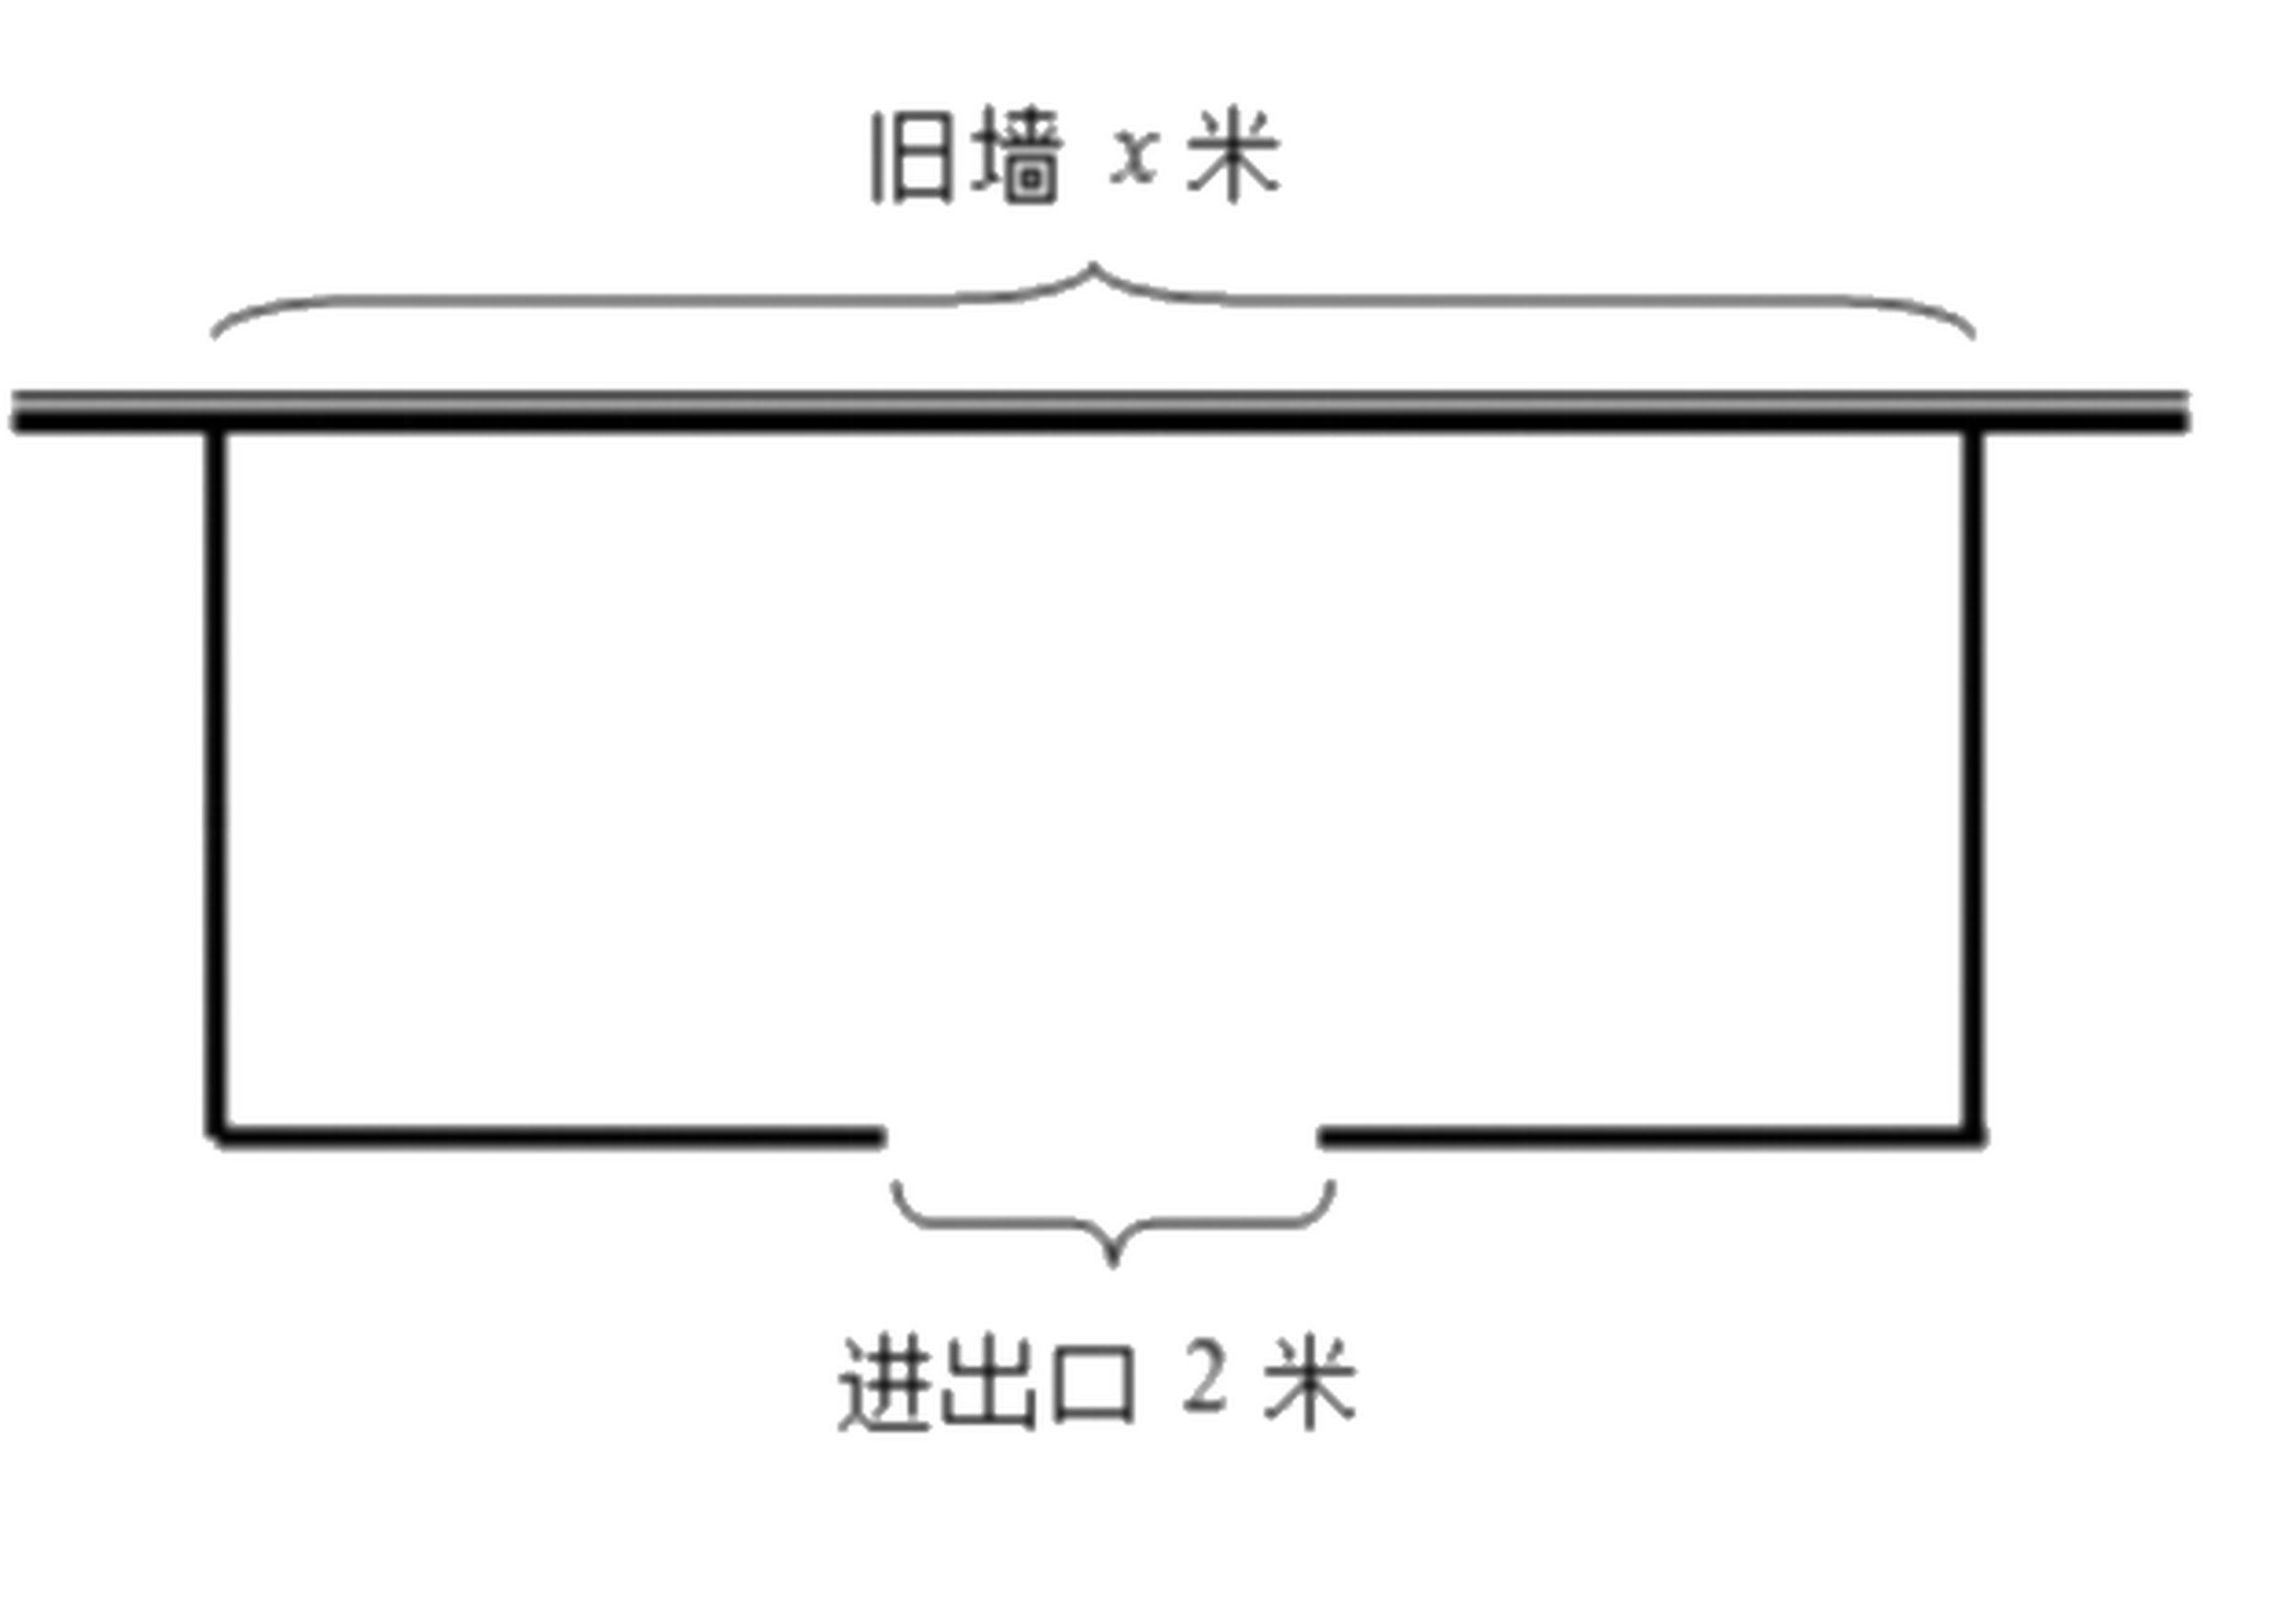
\includegraphics[width=0.60\textwidth]{figures/gao144_q17.png}
\end{center}

(1) 写出总费用 $y$ 关于 $x$ 的表达式;

(2) 试确定 $x$，使修建此矩形场地围墙的总费用最小，并求出最小总费用.

\ifanswer
\solbegin
\step{(1) 设矩形的另一边长为 $a$ 米，}
\step{则 $y=45x+180(x-2)+180\times2a=225x+360a-360$，}
\step{由已知 $xa=360$，得 $a=\dfrac{360}{x}$，所以 $y=225x+\dfrac{360^2}{x}-360(x>0)$;}
\step{(2) 因为 $x>0$，所以 $225x+\dfrac{360^2}{x}\geqslant2\sqrt{225x\cdot\dfrac{360^2}{x}}=10800$，}
\step{所以 $y=225x+\dfrac{360^2}{x}-360\geqslant10440$，}
\step{当且仅当 $225x=\dfrac{360^2}{x}$，即 $x=24$ 时取等号，}
\step{所以当 $x=24$ 米时，修建围墙的总费用最小，最小总费用是 10440 元.}
\solend
\fi

\item 已知集合 $A=\{a_1,a_2,\cdots,a_k\}(k\geqslant2)$，其中 $a_i\in\Z(i=1,2,\cdots,k)$. 定义：若对任意的 $x\in A$，必有 $-x\notin A$，则称集合 $A$ 具有性质 $G$. 由 $A$ 中元素可构成两个点集 $P$ 和 $Q$，$P=\{(x,y)\mid x\in A,y\in A,x+y\in A\}$，$Q=\{(x,y)\mid x\in A,y\in A,x-y\in A\}$，其中 $P$ 有 $m$ 个元素，$Q$ 中有 $n$ 个元素.

(1) 已知集合 $K=\{-1,2,3\}$，判断 $K$ 是否具有性质 $G$; 并写出 $K$ 对应的集合 $P$ 和集合 $Q$;

(2) 若集合 $A=\{1,2,3,4,5,6,7,8,9,10\}$，求对应集合 $Q$ 的元素个数; 一般地，若集合 $A$ 具有性质 $G$，且有 $k$ 个元素，猜测对应的集合 $Q$ 的元素最大个数，并说明理由;

(3) 若集合 $A$ 具有性质 $G$，猜测 $m,n$ 的大小并说明理由.

\ifanswer
\solbegin
\step{(1) 因为 $K=\{-1,2,3\},1,-2,-3$ 都不属于集合 $K$，}
\step{所以集合 $K$ 具有性质 $G$，}
\step{对应集合 $P=\{(-1,3),(3,-1)\},Q=\{(2,-1),(2,3)\}$;}
\step{(2) $A=\{1,2,3,4,5,6,7,8,9,10\}$，则对应集合 $Q$ 中的元素为:}
\step{$(2,1),(3,2),\cdots,(9,8),(10,9)$,}
\step{$(3,1),(4,2),\cdots,(9,7),(10,8)$,}
\step{$(4,1),(5,2),\cdots,(9,6),(10,7)$,}
\step{$\cdots$}
\step{$(9,1),(10,2)$,}
\step{$(10,1)$,}
\step{共有 $9+8+7+\cdots+2+1=45$ 个元素，即对应集合 $Q$ 的元素个数 45;}
\step{集合 $A$ 有 $k$ 个元素，猜测对应的集合 $Q$ 的最大个数为 $\dfrac{k^2-k}{2}$. 理由如下:}
\step{由题意得集合 $A$ 的元素构成有序数对 $(a_i,a_j)(i,j\in\N^*,i\leqslant k,j\leqslant k)$，}
\step{共有 $k^2$ 个，因为 $0\notin A$，所以 $(a_i,a_i)\notin Q$，}
\step{又因为 $a\in A$ 时，$-a\notin A$，所以 $(a_i,a_j)\in Q$ 时，$(a_j,a_i)\notin Q$，}
\step{所以集合 $Q$ 的元素个数为 $\dfrac{k^2-k}{2}$ 个，}
\step{(3) 当集合 $A$ 具有性质 $G$ 时，}
\step{①对于 $(a,b)\in P$，由定义得 $a\in A,b\in A,a+b\in A$，}
\step{又因为集合 $A$ 具有性质 $G$，所以 $(a+b,a)\in Q$，}
\step{如果 $(a,b),(c,d)$ 是 $P$ 中的不同元素，}
\step{那么 $a=c,b=d$ 中至少有一个不成立，}
\step{于是 $b=d,a+b=c+d$ 中至少有一个不成立，}
\step{故 $(a+b,b)$ 和 $(c+d,d)$ 也是 $Q$ 中不同的元素，}
\step{可见 $P$ 的元素个数不多于 $Q$ 的元素个数，即 $m\leqslant n$;}
\step{②对于 $(a,b)\in Q$，由定义得 $a\in A,b\in A,a-b\in A$，}
\step{又因为集合 $A$ 具有性质 $G$，则 $(a-b,b)\in P$，}
\step{如果 $(a,b),(c,d)$ 是 $Q$ 中的不同元素，}
\step{那么 $a=c,b=d$ 中至少有一个不成立，}
\step{于是 $b=d,a-b=c-d$ 中至少有一个不成立，}
\step{故 $(a-b,b)$ 和 $(c-d,d)$ 也是 $P$ 中不同的元素，}
\step{可见 $Q$ 的元素个数不多于 $P$ 的元素个数，即 $n\leqslant m$，}
\step{由①②得 $m=n$.}
\solend
\fi

\end{enumerate}

\end{document}
"
%
% ① 原始材料：微信公众号"魔都数学加油站"文章，连载"27学年高一144"，原文标题
% "27学年高一144——2026-2027年上海市风华中学高一上期中"；
% 原文链接：https://mp.weixin.qq.com/s/ylUlbXfudWOYC-jlH3jyjw 。
% 正文为 10 张 PNG 页，题目下印【解析】，为讲评版。
% 各页分辨率：01/02/03/05/06/07/09/10 为 2560×3620，04/08 为 4762×6735。
% 题目、解析均据原图转录；卷面粉红色水印"魔都数学加油站"及公众号页脚未录入。
% 全卷插图情况：Q17 有一幅矩形场地示意图（旧墙 x 米 / 进出口 2 米），从 07 页裁出、
%   去粉色水印去色 4× LANCZOS 放大存 figures/gao144_q17.png；其余 9 页逐页通读
%   确认无题目配图、无表格、亦无"题干写如图而源码漏图"一处。
%
% 卷首标题：原卷印作"2026-2027 年风华中学高一上期中"，年份区间按全稿惯例排 en dash；
% 原卷卷面未印副标题，本稿按同期中卷（高一140／141／143）知识模块口径补出
% "集合与常用逻辑用语、不等式、函数"：集合与逻辑见 Q3、Q7、Q9、Q10、Q12、Q16、Q18，
% 不等式见 Q6、Q11、Q13、Q14、Q15、Q17，函数见 Q4、Q5、Q8、Q9。
%
% 题号体例：本卷共 16 题——一、填空题 3—10（8 题）、二、选择题 11—13（3 题）、
% 三、解答题 14—18（5 题）。三节分别 \setcounter{enumi}{2}／{10}／{13}。
% 原卷从第 3 题起、无第 1、2 题，本稿保留原题号；全卷无附加题节。
%
% ② 与原卷的排版差异：
%   ① 原文从第 3 题起，本稿保留原题号；共 16 题三节；
%   ② 原卷 15 题题下印【解析】，唯 Q11 未印【解析】、只把答案"（ BD ）"直接印在
%      题干括号内（放大 04 页 A/B 选项与 05 页 C/D 选项衔接处确认，见 ⑤）；
%      按 高一128／94／106／140 成例：Q11 试卷版括号留空 \mbox{（\quad）}、
%      答案版另提 \ans{$BD$}、不补造原卷没有的解析；其余 15 题印【解析】、
%      括号内一律留空、不另提 \ans{}（Q12 选 C、Q13 选 B 在解析末句"故选 …"）；
%      答案版【答案】/【解析】标记数 = 16（1 个 \ans + 15 个 \solbegin）= 全卷题数；
%      正文 Q11 对应处另有 % 注；
%   ③ 原卷卷面未印副标题，本稿按知识模块口径补出；
%   ④ 原卷填空横线按全稿惯例排 \blankline[4.4em]；选择题括号排 \mbox{（\quad）}，
%      选项段前按惯例加 \keepwithprev；解答题不留作答区、不加 \anspace
%      （原卷为讲评版，与 129／131／132／133／136／140／141／143 同）；
%   ⑤ 数集：Q9 题干与解析"a,b∈R"、Q12 题干"U=R"、Q15 题干"x,y∈R"原卷印
%      斜体或黑板粗体 R，Q18 题干"a_i∈Z"印黑板粗体 Z、Q18 解析"i,j∈N*"印
%      黑板粗体 N，按全稿惯例统一改 \R／\Z／\N^*；绝对值排 \lvert…\rvert，
%      集合描述竖线排 \mid；不等号按全稿惯例排 \leqslant／\geqslant；
%      补集照原卷上划线排 \overline{A}／\overline{B}；空集记号 \varnothing；
%   ⑥ 子题标号 (1)(2)(3) 原卷印半角括号，照录；圈数字 ①② 在正文（文本模式）
%      按原卷照录（Q15、Q18 解析），未进数学式；数学式内半角逗号照录
%      （Q12 解析"$A=(1,2),B=(0,6)$"、Q18 解析"$(a_i,a_j)(i,j\in\N^*,i\leqslant k,j\leqslant k)$"、
%      Q15 解析"$x=1,y=-1$"、Q18 解析"$a=c,b=d$"等，为全稿惯例、非笔误）；
%      全卷行末西文句点照录为 ASCII `.`；行中全角逗号／顿号照录；
%      Q18 解析集合描述中的"或"用 \text{ 或 } 置于数学式内；
%   ⑦ 题干中的中文弯引号按原卷照录（Q3 的" x∈A "／" x∈B "与 Q15 (2) 的命题
%      引号，含引号内空格），注释内一律 ASCII 引号；
%   ⑧ Q17 配图：题干写"如图所示"，配图居中排在题干之后、子问之前，三版都出；
%      在 Q17 \item 之前加 \needvspace{10cm} 把"题干＋图"整块推走。Q17 是
%      "三、解答题"节内第 4 题（非节首题），故守卫放在 \item 之前而非 \bigsec
%      之前不会让节标题孤落页末（B 类）；三版切页审计均"合计异常：无"；
%   ⑨ 跨页续印按题合并：Q3 在 01 页；Q4/5/6 在 01 页（Q6 解析续到 02 页顶）；
%      Q7/8/9 在 02 页（Q9 题干跨 02→03）；Q10 在 03 页、解析跨 03→04（很长，
%      按余数分组 A₁/A₂/A₃）；Q11 在 04 页（"二、选择题"节标题也在 04 页下部）、
%      Q12/13 在 05 页（"三、解答题"标题在 05 页下部）；Q14 在 05 页末、解析在 06 页；
%      Q15/16 在 06 页（Q16 续到 07 页）；Q17 在 07 页；Q18 在 08 页、解析跨
%      08/09/10 页（性质 G 压轴，3 问，很长）；本稿按题连排，不丢行、不并折行；
%   ⑩ Q8 解析"法一：""法二："两处标签经放大 02 页逐字确认原卷均印红色
%      （见 ⑤）；按全稿惯例（高一53 成例）不引入红色、均照录为黑体着色
%      \stepm{法一：}{…}／\stepm{法二：}{…}，不改 common.sty；
%      文件头在此注明原卷为红色；
%   ⑪ "图像／图象"逐处核：全卷未出现"图像"或"图象"字样，无统一问题；
%   ⑫ \left…\right 不得拆到不同 $…$ 组；cases 块整体算一个印刷行；
%      Q4 分式与 8×(-3/4) 同一 $…$ 组，Q13 的 \left(\frac1x+\frac2y\right) 同理。
%
% ③ 行数复核：一条 \step／\stepm 行 = 原卷解析的一个印刷行，cases 块作一个印刷行计。
%   逐题数（含 \stepm）：Q3：3；Q4：1；Q5：1；Q6：5；Q7：4；Q8：8（6 \step
%   ＋ 2 \stepm，法一/法二标签各占 1 行）；Q9：6；Q10：23；Q11：0（原卷无解析，
%   答案另提 \ans{$BD$}）；Q12：5；Q13：3；Q14：5；Q15：8；Q16：7；Q17：7；
%   Q18：32。合计 116 条 \step ＋ 2 条 \stepm ＝ 118 个印刷行，与原卷逐题相等。
%   全卷 15 题设 \solbegin…\solend ＋ Q11 一处 \ans{}，答案版【答案】/【解析】
%   标记数 = 16 = 全卷题数。
%
% ④ 判别式／子集符号结论（逐处放大原图照录、不得统一）：
%   判别式全卷 2 处，逐页放大扫过 10 页确认（Q4 为分式指数化简、不含判别式）：
%     · Q9【解析】"所以 △=a^2-4b=0" 原卷印细线、扁等边三角（宽≈高、笔画细，
%       放大见 /tmp/gao144fh/z_q9_tri.png、z_tri_Q9.png），照录 \triangle；
%     · Q15 (2)【解析】cases 块"Δ=(a-2)^2-4(a-2)≤0" 原卷印等腰偏高、粗笔画
%       三角（高>宽，放大见 z_q15_tri.png、z_tri_Q15.png），照录 \Delta；
%   两形不同、全卷混用，逐处照录不统一（参照 高一142 头注④口径）。
%   子集符号全卷 4 处，逐处放大核：
%     · Q3 解析"所以 B⊆A"、Q16 (1) 解析"所以 B⊆A" 原卷均印带下划线的 ⊆
%       （z_q3_symbol.png、z_q16_subset2.png），照录 \subseteq；
%     · Q12 选项 B"$\overline{A}\subset B$" 原卷印单线 ⊂（z_q12_opts2.png），
%       照录 \subset；Q12 解析"$\overline{A}=(-\infty,1]\cup[2,+\infty)\not\subset B$"
%       原卷印单线带斜杠 ⊄（z_q12_notsym3.png），照录 \not\subset；
%   \subset 与 \subseteq 混用，逐处照录不统一。补集照原卷上划线 \overline{A}／
%   \overline{B}，空集 \varnothing，数集 \R／\Z／\N^* 归一见 ② ⑤。
%
% ⑤ 存疑／特殊体例（主会话逐处放大原图复核确认，照录未改，正文对应处另有 % 注）：
%   1. 第 11 题原卷把答案"（ BD ）"直接印在题干括号内、题下未印【解析】
%      （放大 04 页 A/B 选项与 05 页 C/D 选项衔接处确认：05 页顶 C/D 选项后
%      直接接第 12 题）。按 高一128／94／106／140 成例括号留空、另提
%      \ans{$BD$}，不补造解析（不编造）。
%   2. 第 10 题题干"集合 $S$ 为集合 $M=\{1,2,3,4,\cdots,2026\}$，的子集"在
%      集括号与"的子集"之间原卷多印一个全角逗号（放大 03 页确认），
%      按存疑照录未删，正文对应处另有 % 注。
%   3. 第 8 题解析"法一：""法二："两处原卷均印红色（放大 02 页逐字确认），
%      按全稿惯例不引入红色、两处均照录为黑体着色 \stepm（见 ② ⑩）。
%   全卷除此 3 条外未发现其它笔误／自相矛盾处。
%
% ⑥ 跨页续印按题合并说明：见 ② ⑨。
%
\documentclass[a4paper,11pt]{article}
\usepackage{common}

\begin{document}

\examtitlest[3]{2026--2027 年风华中学高一上期中}{集合与常用逻辑用语、不等式、函数}

\bigsec{一、填空题}

\begin{enumerate}
\setcounter{enumi}{2}

\item $A=\{x\mid x>4\}$，$B=\{x\mid x>a\}$，若命题 “ $x\in A$ ” 是命题 “ $x\in B$ ” 的必要条件，则 $a$ 的取值范围是\blankline[4.4em].

\ifanswer
\solbegin
\step{因为 “ $x\in A$ ” 是命题 “ $x\in B$ ” 的必要条件，所以 $B\subseteq A$，}% 子集符号原卷印带下划线 $\subseteq$，照录
\step{因为 $A=\{x\mid x>4\}$，$B=\{x\mid x>a\}$，所以 $a\geqslant4$，}
\step{所以 $a$ 的取值范围是 $\{a\mid a\geqslant4\}$.}
\solend
\fi

\item 已知 $a>0,b>0$，化简式子：$\dfrac{8a^{\frac34}b^3}{\left(a^{\frac16}b^{\frac32}\right)\left(-\dfrac43 a^{\frac1{12}}b^{\frac12}\right)}=$\blankline[4.4em].

\ifanswer
\solbegin
\step{$\dfrac{8a^{\frac34}b^3}{\left(a^{\frac16}b^{\frac32}\right)\left(-\dfrac43 a^{\frac1{12}}b^{\frac12}\right)}=8\times\left(-\dfrac34\right)a^{\frac34-\frac16-\frac1{12}}b^{3-\frac32-\frac12}=-6a^{\frac12}b=-6b\sqrt a$.}
\solend
\fi

\item 已知 $\lg2=a$，$\lg3=b$，则 $\log_5 6=$\blankline[4.4em]（结果用 $a,b$ 表示）.

\ifanswer
\solbegin
\step{$\log_5 6=\dfrac{\lg6}{\lg5}=\dfrac{\lg2+\lg3}{1-\lg2}=\dfrac{a+b}{1-a}$.}
\solend
\fi

\item 若关于 $x$ 的不等式 $ax>b$ 的解集为 $(-\infty,2)$，则不等式 $bx+a>0$ 的解集为\blankline[4.4em].

\ifanswer
\solbegin
\step{因为不等式 $ax>b$ 的解集为 $(-\infty,2)$，所以 $a<0$，}
\step{所以由不等式解得 $x<\dfrac ba$，所以 $\dfrac ba=2$，即 $b=2a$，}
\step{代入不等式 $bx+a>0$，得 $2ax+a>0$，}
\step{因为 $a<0$，所以不等式化为 $2x+1<0$，解得 $x<-\dfrac12$，}
\step{故不等式的解集为 $\left(-\infty,-\dfrac12\right)$.}
\solend
\fi

\item 如果集合 $A=\{x\mid x^2-4x\leqslant0\}$，$B=\{x\mid x^2+ax+b\leqslant0\}$，$A\cap B=\{x\mid3\leqslant x\leqslant4\}$，$A\cup B=\{x\mid0\leqslant x\leqslant5\}$，则 $a+b=$\blankline[4.4em].

\ifanswer
\solbegin
\step{由题意得 $A=\{x\mid x^2-4x\leqslant0\}=[0,4]$，}
\step{又因为 $A\cap B=\{x\mid3\leqslant x\leqslant4\}$，$A\cup B=\{x\mid0\leqslant x\leqslant5\}$，}
\step{所以 $B=\{x\mid3\leqslant x\leqslant5\}$，即方程 $x^2+ax+b=0$ 的两根为 $3,5$，}
\step{由韦达定理得 $\begin{cases}3+5=-a\\3\times5=b\end{cases}$，解得 $a=-8$，$b=15$，所以 $a+b=15-8=7$.}
\solend
\fi

% 第 8 题：原卷"法一：""法二："两处标签均印红色（8× 放大确认）；按交办口径
% "法一"用普通 \step、"法二："排 \stepm（加粗着色、不引红色），见头注 ② ⑩／⑤
\item 若关于 $x$ 的方程 $\lvert x-1\rvert+\lvert\pi-x\rvert=\pi-1$ 的解集为\blankline[4.4em].

\ifanswer
\solbegin
\stepm{法一：}{因为 $\lvert x-1\rvert+\lvert\pi-x\rvert=\begin{cases}x-1+x-\pi,x\geqslant\pi\\\pi-1,1<x<\pi\\1-x+\pi-x,x\leqslant1\end{cases}=\begin{cases}2x-1-\pi,x\geqslant\pi\\\pi-1,1<x<\pi\\1+\pi-2x,x\leqslant1\end{cases}$.}
\step{当 $x\geqslant\pi$ 时，令 $2x-1-\pi=\pi-1$，得 $x=\pi$；}
\step{当 $1<x<\pi$ 时，$\lvert x-1\rvert+\lvert\pi-x\rvert=\pi-1$ 恒成立；}
\step{当 $x\leqslant1$ 时，令 $1+\pi-2x=\pi-1$，得 $x=1$.}
\step{综上所述，方程 $\lvert x-1\rvert+\lvert\pi-x\rvert=\pi-1$ 的解集为 $[1,\pi]$.}
\stepm{法二：}{因为 $\lvert x-1\rvert+\lvert\pi-x\rvert\geqslant\lvert x-1+\pi-x\rvert=\pi-1$，}
\step{当且仅当 $(x-1)(\pi-x)\geqslant0$ 时取等号，}
\step{故方程 $\lvert x-1\rvert+\lvert\pi-x\rvert=\pi-1$ 的解集为 $[1,\pi]$.}
\solend
\fi

% 第 9 题：题干跨 02→03 页；解析判别式原卷印细线扁等边三角 $\triangle$，照录
\item 已知函数 $f(x)=x^2+ax+b(a,b\in\R)$ 和 $x$ 轴有且只有一个交点，若关于 $x$ 的不等式 $f(x)<c$ 的解集为 $(m,m+6)$，则 $c=$\blankline[4.4em].

\ifanswer
\solbegin
\step{因为函数 $f(x)=x^2+ax+b(a,b\in\R)$ 和 $x$ 轴有且只有一个交点，}
\step{所以 $\triangle=a^2-4b=0$，即 $b=\dfrac{a^2}{4}$，}% 判别式原卷印扁等边三角 $\triangle$，照录
\step{不等式 $f(x)<c$ 的解集为 $(m,m+6)$，}
\step{即 $x^2+ax+\dfrac{a^2}{4}-c<0$ 的解集为 $(m,m+6)$，}
\step{所以方程 $x^2+ax+\dfrac{a^2}{4}-c=0$ 的两个根为 $x_1=m$，$x_2=m+6$，}
\step{所以 $\begin{cases}x_1+x_2=2m+6=-a\\x_1x_2=m(m+6)=\dfrac{a^2}{4}-c\end{cases}$，消去 $m$ 得 $\dfrac{a^2}{4}-9=\dfrac{a^2}{4}-c$，解得 $c=9$.}
\solend
\fi

% 第 10 题：原卷题干在集括号与"的子集"之间多印一个全角逗号，照录未改（存疑，见头注 ⑤）
\item 已知集合 $S$ 为集合 $M=\{1,2,3,4,\cdots,2026\}$，的子集，并且集合 $S$ 中任意两个元素之和不能被 3 整除，则集合 $S$ 中元素个数的最大值为\blankline[4.4em].

\ifanswer
\solbegin
\step{对于集合 $M=\{1,2,3,4,\cdots,2026\}$，}
\step{所有被 3 除余数为 0 的元素组成的集合为 $A_3=\{3,6,9,\cdots,2025\}$，}
\step{元素个数为 675;}
\step{所有被 3 除余数为 1 的元素组成的集合为 $A_1=\{1,4,7,\cdots,2026\}$，}
\step{元素个数为 676;}
\step{所有被 3 除余数为 2 的元素组成的集合为 $A_2=\{2,5,8,\cdots,2024\}$，}
\step{元素个数为 675;}
\step{集合 $S$ 中任意两个元素之和不能被 3 整除，}
\step{若两个元素分别来自 $A_1$ 和 $A_2$，则两数之和除以 3 的余数为 $1+2=3\equiv0$，}
\step{即和能被 3 整除，}
\step{所以 $S$ 不能同时包含 $A_1$ 和 $A_2$ 中的元素，}
\step{即 $S$ 最多只能选取 $A_1$、$A_2$ 一个集合中的全部元素;}
\step{若两个元素都来自 $A_3$，则两数之和除以 3 的余数为 $0+0=0$，即和能被 3 整除，}
\step{所以 $S$ 中最多包含 $A_3$ 中的 1 个元素;}
\step{对 $A_1$ 内的任意两个元素，其和除以 3 的余数为 $1+1=2$，不能被 3 整除;}
\step{$A_1$ 中元素与 $A_3$ 中元素的和除以 3 余数为 $1+0=1$，不能被 3 整除，}
\step{所以 $A_1$ 的全部元素与 $A_3$ 中的任意 1 个元素的组合满足题意;}
\step{对 $A_2$ 内的任意两个元素，其和除以 3 的余数为 $2+2=4\equiv1$，不能被 3 整除;}
\step{$A_2$ 中元素与 $A_3$ 中元素的和除以 3 的余数为 $2+0=2$，不能被 3 整除，}
\step{所以 $A_2$ 的全部元素与 $A_3$ 中任意 1 个元素的组合也满足题意.}
\step{故若选取 $A_2$ 全部元素加 1 个 $A_3$ 元素，总个数为 $675+1=676$;}
\step{选取 $A_1$ 全部元素加 1 个 $A_3$ 元素，总个数为 $676+1=677$;}
\step{所以集合 $S$ 中元素个数的最大值为 677.}
\solend
\fi

\end{enumerate}

\bigsec{二、选择题}

\begin{enumerate}
\setcounter{enumi}{10}

% 第 11 题：原卷把答案"（ BD ）"直接印在题干括号内、题下无【解析】（放大 04 页 A/B 选项
% 与 05 页 C/D 选项衔接处确认）。按 高一128／94／106／140 成例：试卷版括号留空、
% 答案版另提 \ans{$BD$}、不补造原卷没有的解析（不编造）。
\item 已知实数 $a,b$，下列四个不等式中正确的是\mbox{（\quad）}

\keepwithprev
A. $a+\dfrac1a\geqslant2$\qquad B. $\sqrt{a^2+2}+\dfrac{1}{\sqrt{a^2+2}}\geqslant2$

C. $\dfrac{a+b}{2}\leqslant\sqrt{ab}$\qquad D. $a^2+b^2\geqslant2ab$

\ifanswer
\ans{$BD$}
\fi

\item 若全集 $U=\R$，$A=\{x\mid x^2-3x+2<0\}$，$B=\{x\mid0<x<6\}$，则\mbox{（\quad）}

\keepwithprev
A. $A\cap B=B$\qquad B. $\overline{A}\subset B$\qquad C. $A\cap\overline{B}=\varnothing$\qquad D. $A\cup B=A$

\ifanswer
\solbegin
\step{由 $x^2-3x+2<0$，则 $A=(1,2),B=(0,6)$，所以 $A\cap B=(1,2)=A,A$ 错误;}
\step{$\overline{A}=(-\infty,1]\cup[2,+\infty)\not\subset B$，$B$ 错误;}
\step{$\overline{B}=(-\infty,0]\cup[6,+\infty)$，所以 $A\cap\overline{B}=\varnothing,C$ 正确;}
\step{$A\cup B=(0,6)\ne A,D$ 错误.}
\step{故选 $C$.}
\solend
\fi

\item 已知正数 $x$、$y$ 满足 $\dfrac1x+\dfrac2y=1$，不等式 $3x+2y-1>m$ 恒成立，则实数 $m$ 的取值范围是\mbox{（\quad）}

\keepwithprev
A. $(-\infty,4+6\sqrt2)$\qquad B. $(-\infty,6+4\sqrt3)$\qquad C. $(6+4\sqrt2,+\infty)$\qquad D. $(8+4\sqrt3,+\infty)$

\ifanswer
\solbegin
\step{$3x+2y=(3x+2y)\left(\dfrac1x+\dfrac2y\right)=7+\dfrac{6x}{y}+\dfrac{2y}{x}\geqslant7+2\sqrt{\dfrac{6x}{y}\cdot\dfrac{2y}{x}}=7+4\sqrt3$，}
\step{当且仅当 $\dfrac{6x}{y}=\dfrac{2y}{x}$，即 $y=\sqrt3x=\sqrt3+2$ 时取等号，}
\step{故要使原式成立，只需 $m<6+4\sqrt3$. 故选 $B$.}
\solend
\fi

\end{enumerate}

\bigsec{三、解答题}

\begin{enumerate}
\setcounter{enumi}{13}

\item 解关于 $x$ 的不等式：

(1) $x^2-2\lvert x\rvert-3>0$；

(2) $\dfrac{2x-1}{x+2}<1$.

\ifanswer
\solbegin
\step{(1) 原不等式等价于 $(\lvert x\rvert-3)(\lvert x\rvert+1)>0$，}
\step{$\lvert x\rvert+1>0$，故 $\lvert x\rvert>3$，解得 $x<-3$ 或 $x>3$，}
\step{故不等式的解集为 $(-\infty,-3)\cup(3,+\infty)$.}
\step{(2) 已知 $\dfrac{2x-1}{x+2}<1$，则 $\dfrac{2x-1}{x+2}-1<0$，即 $\dfrac{x-3}{x+2}<0$，}
\step{等价于 $(x-3)(x+2)<0$，解得 $-2<x<3$，故不等式的解集为 $(-2,3)$.}
\solend
\fi

\item (1) 已知 $x,y\in\R$，比较 $x^2+y^2$ 与 $2x-2y-2$ 的大小.

(2) “不等式 $(a-2)x^2+(a-2)x+1\geqslant0$ 对一切实数恒成立” 是假命题，求实数 $a$ 的取值范围.

\ifanswer
\solbegin
\step{(1) $x^2+y^2-(2x-2y-2)=x^2+y^2-2x+2y+2=(x-1)^2+(y+1)^2\geqslant0$，}
\step{故 $x^2+y^2\geqslant2x-2y-2$，当且仅当 $x=1,y=-1$ 时取等号.}
\step{(2) 先求命题 “$(a-2)x^2+(a-2)x+1\geqslant0$ 对一切实数恒成立” 为真，}
\step{①当 $a-2=0$ 时，即 $a=2$，不等式化为 $1\geqslant0$，成立，符合条件，}
\step{②当 $a-2\ne0$ 时，则 $\begin{cases}a-2>0\\\Delta=(a-2)^2-4(a-2)\leqslant0\end{cases}$，解得 $2<a\leqslant6$，}% 判别式原卷印等腰偏高三角 $\Delta$，照录
\step{综上①②，命题为真时 $2\leqslant a\leqslant6$，}
\step{该命题为假命题，则 $a<2$ 或 $a>6$，}
\step{所以实数 $a$ 的取值范围是 $(-\infty,2)\cup(6,+\infty)$.}
\solend
\fi

\item 设集合 $A=\{x\mid-1\leqslant x\leqslant2\}$，$B=\{x\mid m-1<x<2m+1\}$.

(1) 若 $A\cup B=A$，求实数 $m$ 的取值范围;

(2) 若 $B\cap\overline{A}$ 中只有一个整数 $-2$，求实数 $m$ 的取值范围.

\ifanswer
\solbegin
\step{(1) 因为 $A\cup B=A$，所以 $B\subseteq A$，}% 子集符号原卷印带下划线 $\subseteq$，照录
\step{当 $B=\varnothing$ 时，有 $m-1\geqslant2m+1$，解得 $m\leqslant-2$；}
\step{当 $B\ne\varnothing$ 时，有 $\begin{cases}m-1<2m+1\\m-1\geqslant-1\\2m+1\leqslant2\end{cases}$，解得 $0\leqslant m\leqslant\dfrac12$，}
\step{所以实数 $m$ 的取值范围是 $(-\infty,-2]\cup\left[0,\dfrac12\right]$;}
\step{(2) 由集合 $A=\{x\mid-1\leqslant x\leqslant2\}$，得 $\overline{A}=\{x\mid x<-1\text{ 或 }x>2\}$，}
\step{若 $B\cap\overline{A}$ 中只有一个整数 $-2$，则 $B\ne\varnothing$，且满足 $\begin{cases}m-1<2m+1\\-3\leqslant m-1<-2\\-2<2m+1\leqslant3\end{cases}$}
\step{解得 $-\dfrac32<m<-1$，所以实数 $m$ 的取值范围是 $\left(-\dfrac32,-1\right)$.}
\solend
\fi

% 第 17 题配图是"题干＋图"整块；守卫放在 \item 之前（Q17 非节首题，不会让节标题孤落页末）
\needvspace{10cm}
\item 现要围建一个面积为 360 平方米的矩形场地，要求矩形场地的一面利用旧墙（利用旧墙需维修），其它三面围墙要新建，在旧墙的对面的新墙上要留一个宽度为 2 米的进出口，如图所示，已知旧墙的维修费用为 45 元/米，新墙的造价为 180 元/米，设利用的旧墙的长度为 $x$ 米，工程总造价为 $y$（单位：元）.

\begin{center}
% 矩形场地示意图取自 07 页右侧，去粉色水印、去色、4× LANCZOS 放大
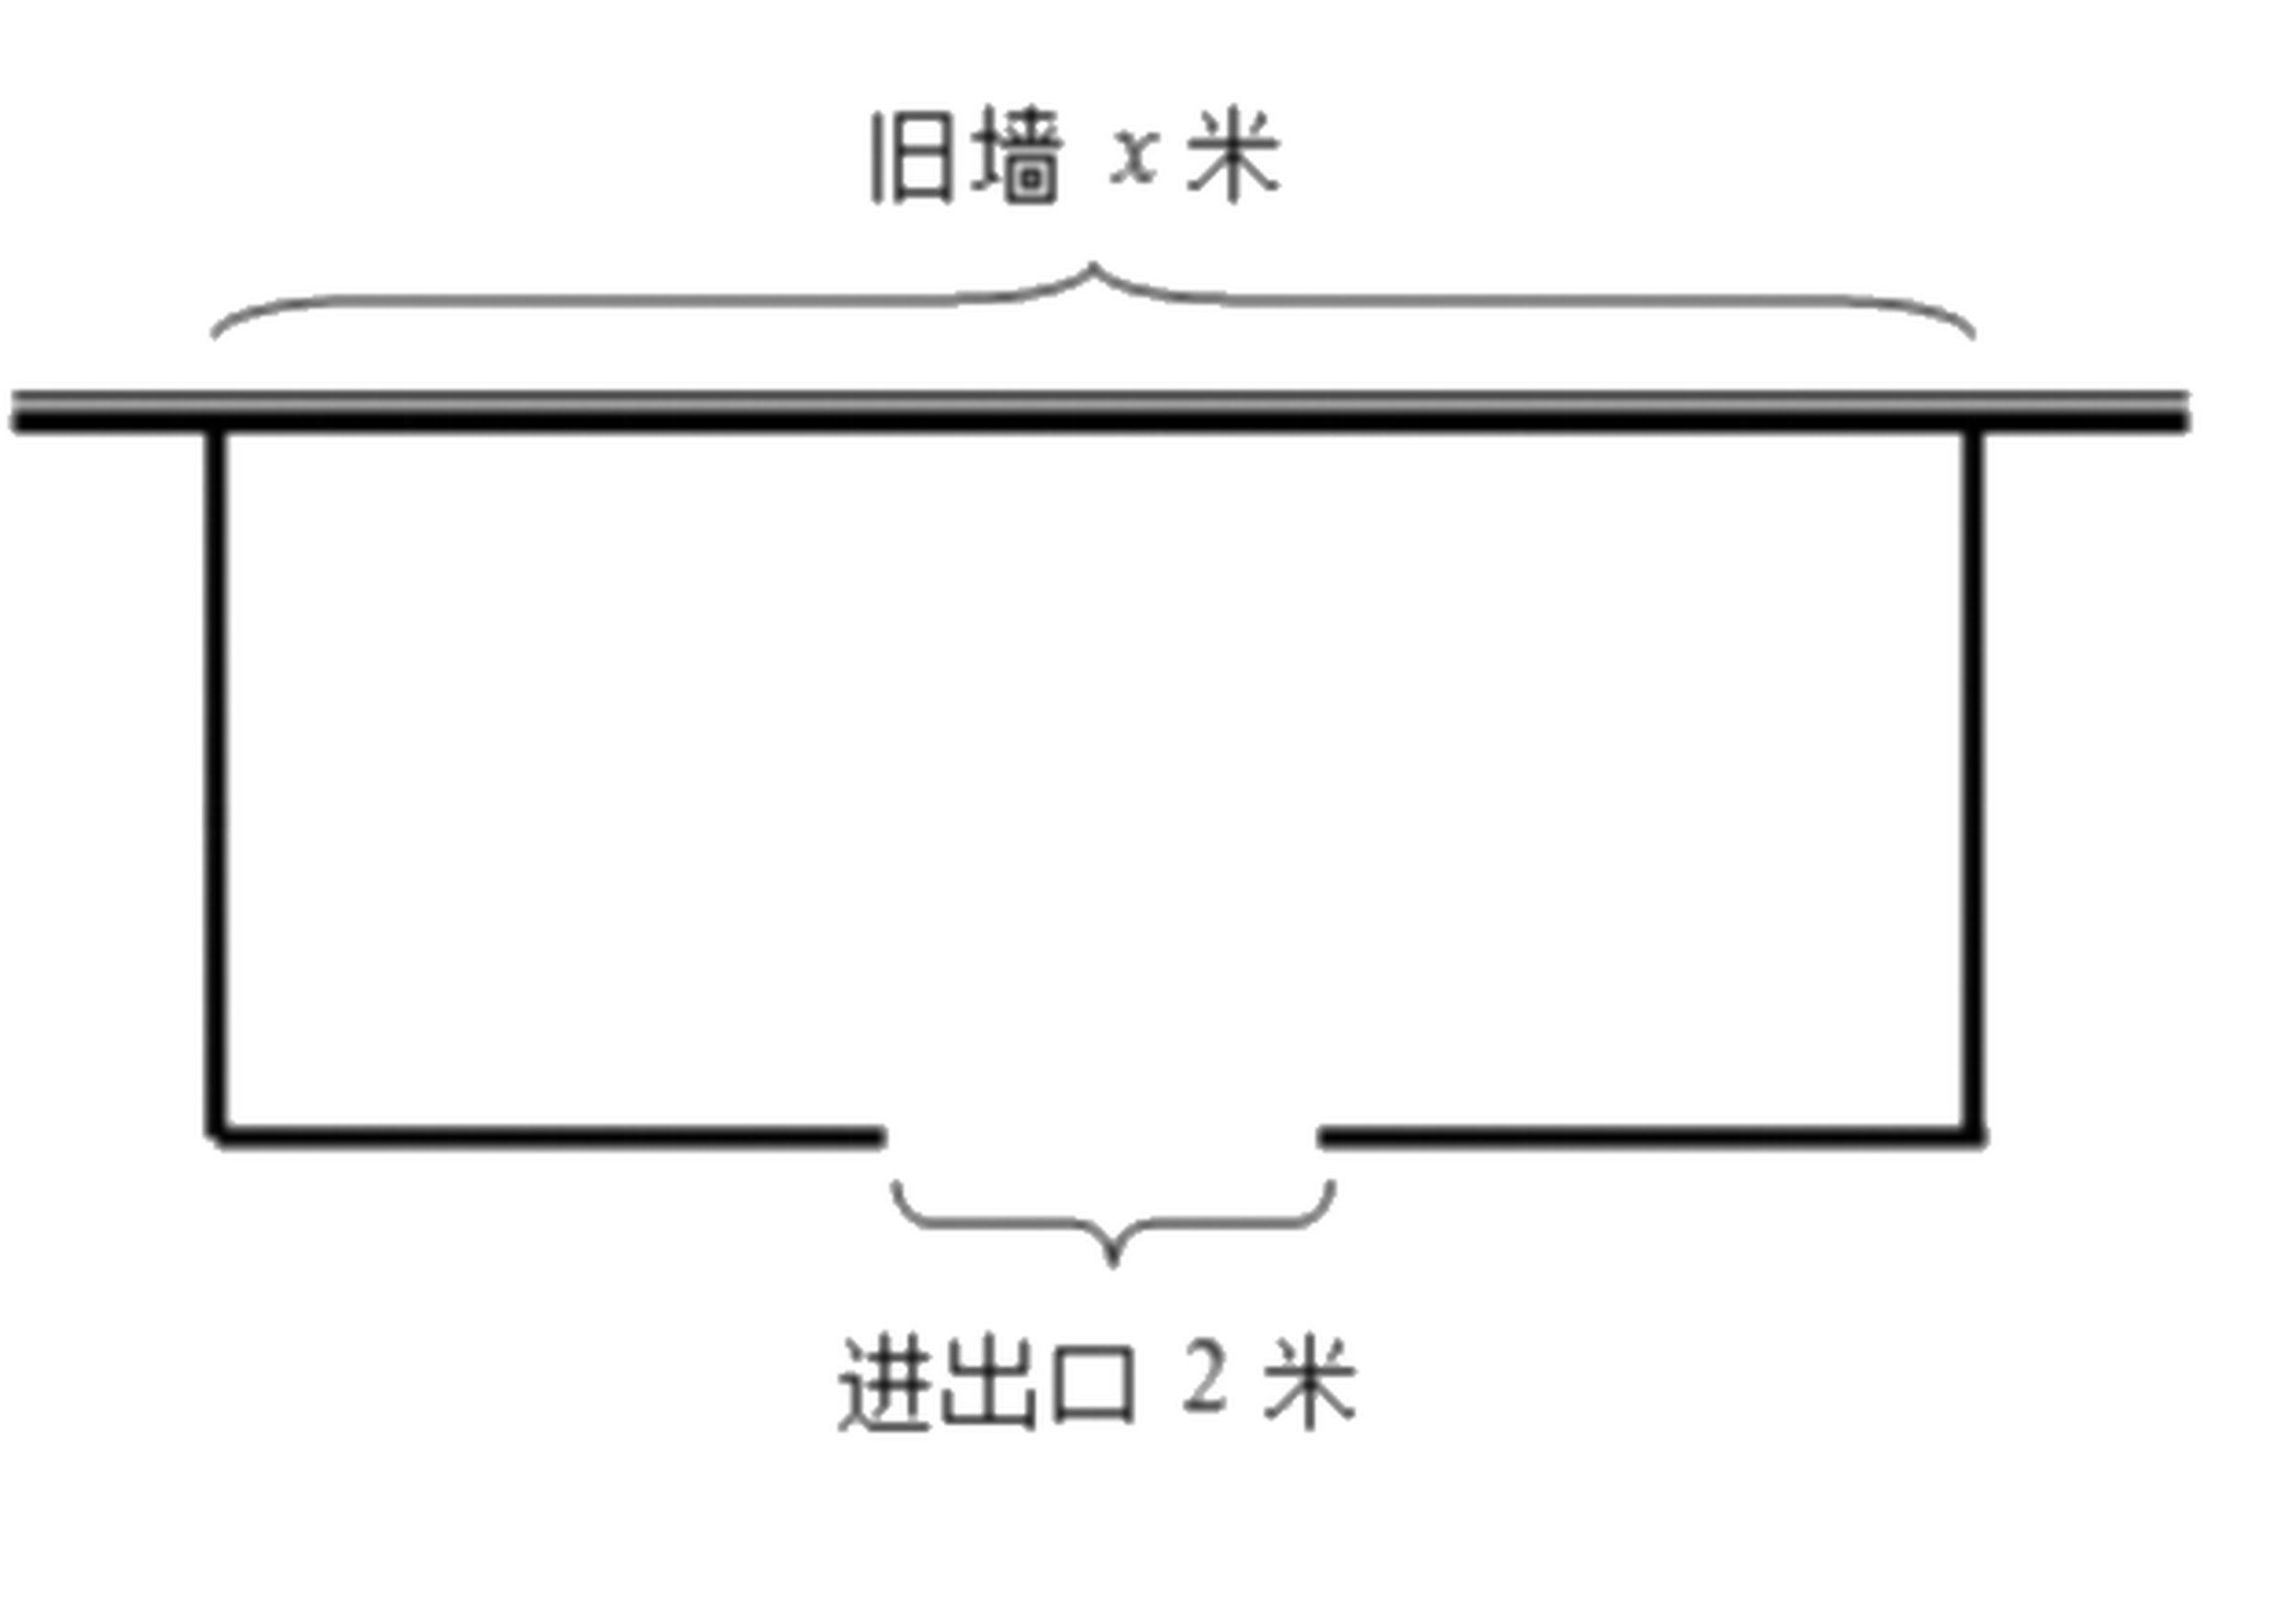
\includegraphics[width=0.60\textwidth]{figures/gao144_q17.png}
\end{center}

(1) 写出总费用 $y$ 关于 $x$ 的表达式;

(2) 试确定 $x$，使修建此矩形场地围墙的总费用最小，并求出最小总费用.

\ifanswer
\solbegin
\step{(1) 设矩形的另一边长为 $a$ 米，}
\step{则 $y=45x+180(x-2)+180\times2a=225x+360a-360$，}
\step{由已知 $xa=360$，得 $a=\dfrac{360}{x}$，所以 $y=225x+\dfrac{360^2}{x}-360(x>0)$;}
\step{(2) 因为 $x>0$，所以 $225x+\dfrac{360^2}{x}\geqslant2\sqrt{225x\cdot\dfrac{360^2}{x}}=10800$，}
\step{所以 $y=225x+\dfrac{360^2}{x}-360\geqslant10440$，}
\step{当且仅当 $225x=\dfrac{360^2}{x}$，即 $x=24$ 时取等号，}
\step{所以当 $x=24$ 米时，修建围墙的总费用最小，最小总费用是 10440 元.}
\solend
\fi

\item 已知集合 $A=\{a_1,a_2,\cdots,a_k\}(k\geqslant2)$，其中 $a_i\in\Z(i=1,2,\cdots,k)$. 定义：若对任意的 $x\in A$，必有 $-x\notin A$，则称集合 $A$ 具有性质 $G$. 由 $A$ 中元素可构成两个点集 $P$ 和 $Q$，$P=\{(x,y)\mid x\in A,y\in A,x+y\in A\}$，$Q=\{(x,y)\mid x\in A,y\in A,x-y\in A\}$，其中 $P$ 有 $m$ 个元素，$Q$ 中有 $n$ 个元素.

(1) 已知集合 $K=\{-1,2,3\}$，判断 $K$ 是否具有性质 $G$; 并写出 $K$ 对应的集合 $P$ 和集合 $Q$;

(2) 若集合 $A=\{1,2,3,4,5,6,7,8,9,10\}$，求对应集合 $Q$ 的元素个数; 一般地，若集合 $A$ 具有性质 $G$，且有 $k$ 个元素，猜测对应的集合 $Q$ 的元素最大个数，并说明理由;

(3) 若集合 $A$ 具有性质 $G$，猜测 $m,n$ 的大小并说明理由.

\ifanswer
\solbegin
\step{(1) 因为 $K=\{-1,2,3\},1,-2,-3$ 都不属于集合 $K$，}
\step{所以集合 $K$ 具有性质 $G$，}
\step{对应集合 $P=\{(-1,3),(3,-1)\},Q=\{(2,-1),(2,3)\}$;}
\step{(2) $A=\{1,2,3,4,5,6,7,8,9,10\}$，则对应集合 $Q$ 中的元素为:}
\step{$(2,1),(3,2),\cdots,(9,8),(10,9)$,}
\step{$(3,1),(4,2),\cdots,(9,7),(10,8)$,}
\step{$(4,1),(5,2),\cdots,(9,6),(10,7)$,}
\step{$\cdots$}
\step{$(9,1),(10,2)$,}
\step{$(10,1)$,}
\step{共有 $9+8+7+\cdots+2+1=45$ 个元素，即对应集合 $Q$ 的元素个数 45;}
\step{集合 $A$ 有 $k$ 个元素，猜测对应的集合 $Q$ 的最大个数为 $\dfrac{k^2-k}{2}$. 理由如下:}
\step{由题意得集合 $A$ 的元素构成有序数对 $(a_i,a_j)(i,j\in\N^*,i\leqslant k,j\leqslant k)$，}
\step{共有 $k^2$ 个，因为 $0\notin A$，所以 $(a_i,a_i)\notin Q$，}
\step{又因为 $a\in A$ 时，$-a\notin A$，所以 $(a_i,a_j)\in Q$ 时，$(a_j,a_i)\notin Q$，}
\step{所以集合 $Q$ 的元素个数为 $\dfrac{k^2-k}{2}$ 个，}
\step{(3) 当集合 $A$ 具有性质 $G$ 时，}
\step{①对于 $(a,b)\in P$，由定义得 $a\in A,b\in A,a+b\in A$，}
\step{又因为集合 $A$ 具有性质 $G$，所以 $(a+b,a)\in Q$，}
\step{如果 $(a,b),(c,d)$ 是 $P$ 中的不同元素，}
\step{那么 $a=c,b=d$ 中至少有一个不成立，}
\step{于是 $b=d,a+b=c+d$ 中至少有一个不成立，}
\step{故 $(a+b,b)$ 和 $(c+d,d)$ 也是 $Q$ 中不同的元素，}
\step{可见 $P$ 的元素个数不多于 $Q$ 的元素个数，即 $m\leqslant n$;}
\step{②对于 $(a,b)\in Q$，由定义得 $a\in A,b\in A,a-b\in A$，}
\step{又因为集合 $A$ 具有性质 $G$，则 $(a-b,b)\in P$，}
\step{如果 $(a,b),(c,d)$ 是 $Q$ 中的不同元素，}
\step{那么 $a=c,b=d$ 中至少有一个不成立，}
\step{于是 $b=d,a-b=c-d$ 中至少有一个不成立，}
\step{故 $(a-b,b)$ 和 $(c-d,d)$ 也是 $P$ 中不同的元素，}
\step{可见 $Q$ 的元素个数不多于 $P$ 的元素个数，即 $n\leqslant m$，}
\step{由①②得 $m=n$.}
\solend
\fi

\end{enumerate}

\end{document}
"
% 紧凑版：xelatex "\def\iscompact{1}% 高一144_风华中学_期中.tex
%   —— 高一上数学"2026-2027 年风华中学高一上期中"（试卷版/答案版/紧凑版）
% 试卷版：xelatex 高一144_风华中学_期中.tex
% 答案版：xelatex "\def\isanswer{1}% 高一144_风华中学_期中.tex
%   —— 高一上数学"2026-2027 年风华中学高一上期中"（试卷版/答案版/紧凑版）
% 试卷版：xelatex 高一144_风华中学_期中.tex
% 答案版：xelatex "\def\isanswer{1}\input{高一144_风华中学_期中.tex}"
% 紧凑版：xelatex "\def\iscompact{1}\input{高一144_风华中学_期中.tex}"
%
% ① 原始材料：微信公众号"魔都数学加油站"文章，连载"27学年高一144"，原文标题
% "27学年高一144——2026-2027年上海市风华中学高一上期中"；
% 原文链接：https://mp.weixin.qq.com/s/ylUlbXfudWOYC-jlH3jyjw 。
% 正文为 10 张 PNG 页，题目下印【解析】，为讲评版。
% 各页分辨率：01/02/03/05/06/07/09/10 为 2560×3620，04/08 为 4762×6735。
% 题目、解析均据原图转录；卷面粉红色水印"魔都数学加油站"及公众号页脚未录入。
% 全卷插图情况：Q17 有一幅矩形场地示意图（旧墙 x 米 / 进出口 2 米），从 07 页裁出、
%   去粉色水印去色 4× LANCZOS 放大存 figures/gao144_q17.png；其余 9 页逐页通读
%   确认无题目配图、无表格、亦无"题干写如图而源码漏图"一处。
%
% 卷首标题：原卷印作"2026-2027 年风华中学高一上期中"，年份区间按全稿惯例排 en dash；
% 原卷卷面未印副标题，本稿按同期中卷（高一140／141／143）知识模块口径补出
% "集合与常用逻辑用语、不等式、函数"：集合与逻辑见 Q3、Q7、Q9、Q10、Q12、Q16、Q18，
% 不等式见 Q6、Q11、Q13、Q14、Q15、Q17，函数见 Q4、Q5、Q8、Q9。
%
% 题号体例：本卷共 16 题——一、填空题 3—10（8 题）、二、选择题 11—13（3 题）、
% 三、解答题 14—18（5 题）。三节分别 \setcounter{enumi}{2}／{10}／{13}。
% 原卷从第 3 题起、无第 1、2 题，本稿保留原题号；全卷无附加题节。
%
% ② 与原卷的排版差异：
%   ① 原文从第 3 题起，本稿保留原题号；共 16 题三节；
%   ② 原卷 15 题题下印【解析】，唯 Q11 未印【解析】、只把答案"（ BD ）"直接印在
%      题干括号内（放大 04 页 A/B 选项与 05 页 C/D 选项衔接处确认，见 ⑤）；
%      按 高一128／94／106／140 成例：Q11 试卷版括号留空 \mbox{（\quad）}、
%      答案版另提 \ans{$BD$}、不补造原卷没有的解析；其余 15 题印【解析】、
%      括号内一律留空、不另提 \ans{}（Q12 选 C、Q13 选 B 在解析末句"故选 …"）；
%      答案版【答案】/【解析】标记数 = 16（1 个 \ans + 15 个 \solbegin）= 全卷题数；
%      正文 Q11 对应处另有 % 注；
%   ③ 原卷卷面未印副标题，本稿按知识模块口径补出；
%   ④ 原卷填空横线按全稿惯例排 \blankline[4.4em]；选择题括号排 \mbox{（\quad）}，
%      选项段前按惯例加 \keepwithprev；解答题不留作答区、不加 \anspace
%      （原卷为讲评版，与 129／131／132／133／136／140／141／143 同）；
%   ⑤ 数集：Q9 题干与解析"a,b∈R"、Q12 题干"U=R"、Q15 题干"x,y∈R"原卷印
%      斜体或黑板粗体 R，Q18 题干"a_i∈Z"印黑板粗体 Z、Q18 解析"i,j∈N*"印
%      黑板粗体 N，按全稿惯例统一改 \R／\Z／\N^*；绝对值排 \lvert…\rvert，
%      集合描述竖线排 \mid；不等号按全稿惯例排 \leqslant／\geqslant；
%      补集照原卷上划线排 \overline{A}／\overline{B}；空集记号 \varnothing；
%   ⑥ 子题标号 (1)(2)(3) 原卷印半角括号，照录；圈数字 ①② 在正文（文本模式）
%      按原卷照录（Q15、Q18 解析），未进数学式；数学式内半角逗号照录
%      （Q12 解析"$A=(1,2),B=(0,6)$"、Q18 解析"$(a_i,a_j)(i,j\in\N^*,i\leqslant k,j\leqslant k)$"、
%      Q15 解析"$x=1,y=-1$"、Q18 解析"$a=c,b=d$"等，为全稿惯例、非笔误）；
%      全卷行末西文句点照录为 ASCII `.`；行中全角逗号／顿号照录；
%      Q18 解析集合描述中的"或"用 \text{ 或 } 置于数学式内；
%   ⑦ 题干中的中文弯引号按原卷照录（Q3 的" x∈A "／" x∈B "与 Q15 (2) 的命题
%      引号，含引号内空格），注释内一律 ASCII 引号；
%   ⑧ Q17 配图：题干写"如图所示"，配图居中排在题干之后、子问之前，三版都出；
%      在 Q17 \item 之前加 \needvspace{10cm} 把"题干＋图"整块推走。Q17 是
%      "三、解答题"节内第 4 题（非节首题），故守卫放在 \item 之前而非 \bigsec
%      之前不会让节标题孤落页末（B 类）；三版切页审计均"合计异常：无"；
%   ⑨ 跨页续印按题合并：Q3 在 01 页；Q4/5/6 在 01 页（Q6 解析续到 02 页顶）；
%      Q7/8/9 在 02 页（Q9 题干跨 02→03）；Q10 在 03 页、解析跨 03→04（很长，
%      按余数分组 A₁/A₂/A₃）；Q11 在 04 页（"二、选择题"节标题也在 04 页下部）、
%      Q12/13 在 05 页（"三、解答题"标题在 05 页下部）；Q14 在 05 页末、解析在 06 页；
%      Q15/16 在 06 页（Q16 续到 07 页）；Q17 在 07 页；Q18 在 08 页、解析跨
%      08/09/10 页（性质 G 压轴，3 问，很长）；本稿按题连排，不丢行、不并折行；
%   ⑩ Q8 解析"法一：""法二："两处标签经放大 02 页逐字确认原卷均印红色
%      （见 ⑤）；按全稿惯例（高一53 成例）不引入红色、均照录为黑体着色
%      \stepm{法一：}{…}／\stepm{法二：}{…}，不改 common.sty；
%      文件头在此注明原卷为红色；
%   ⑪ "图像／图象"逐处核：全卷未出现"图像"或"图象"字样，无统一问题；
%   ⑫ \left…\right 不得拆到不同 $…$ 组；cases 块整体算一个印刷行；
%      Q4 分式与 8×(-3/4) 同一 $…$ 组，Q13 的 \left(\frac1x+\frac2y\right) 同理。
%
% ③ 行数复核：一条 \step／\stepm 行 = 原卷解析的一个印刷行，cases 块作一个印刷行计。
%   逐题数（含 \stepm）：Q3：3；Q4：1；Q5：1；Q6：5；Q7：4；Q8：8（6 \step
%   ＋ 2 \stepm，法一/法二标签各占 1 行）；Q9：6；Q10：23；Q11：0（原卷无解析，
%   答案另提 \ans{$BD$}）；Q12：5；Q13：3；Q14：5；Q15：8；Q16：7；Q17：7；
%   Q18：32。合计 116 条 \step ＋ 2 条 \stepm ＝ 118 个印刷行，与原卷逐题相等。
%   全卷 15 题设 \solbegin…\solend ＋ Q11 一处 \ans{}，答案版【答案】/【解析】
%   标记数 = 16 = 全卷题数。
%
% ④ 判别式／子集符号结论（逐处放大原图照录、不得统一）：
%   判别式全卷 2 处，逐页放大扫过 10 页确认（Q4 为分式指数化简、不含判别式）：
%     · Q9【解析】"所以 △=a^2-4b=0" 原卷印细线、扁等边三角（宽≈高、笔画细，
%       放大见 /tmp/gao144fh/z_q9_tri.png、z_tri_Q9.png），照录 \triangle；
%     · Q15 (2)【解析】cases 块"Δ=(a-2)^2-4(a-2)≤0" 原卷印等腰偏高、粗笔画
%       三角（高>宽，放大见 z_q15_tri.png、z_tri_Q15.png），照录 \Delta；
%   两形不同、全卷混用，逐处照录不统一（参照 高一142 头注④口径）。
%   子集符号全卷 4 处，逐处放大核：
%     · Q3 解析"所以 B⊆A"、Q16 (1) 解析"所以 B⊆A" 原卷均印带下划线的 ⊆
%       （z_q3_symbol.png、z_q16_subset2.png），照录 \subseteq；
%     · Q12 选项 B"$\overline{A}\subset B$" 原卷印单线 ⊂（z_q12_opts2.png），
%       照录 \subset；Q12 解析"$\overline{A}=(-\infty,1]\cup[2,+\infty)\not\subset B$"
%       原卷印单线带斜杠 ⊄（z_q12_notsym3.png），照录 \not\subset；
%   \subset 与 \subseteq 混用，逐处照录不统一。补集照原卷上划线 \overline{A}／
%   \overline{B}，空集 \varnothing，数集 \R／\Z／\N^* 归一见 ② ⑤。
%
% ⑤ 存疑／特殊体例（主会话逐处放大原图复核确认，照录未改，正文对应处另有 % 注）：
%   1. 第 11 题原卷把答案"（ BD ）"直接印在题干括号内、题下未印【解析】
%      （放大 04 页 A/B 选项与 05 页 C/D 选项衔接处确认：05 页顶 C/D 选项后
%      直接接第 12 题）。按 高一128／94／106／140 成例括号留空、另提
%      \ans{$BD$}，不补造解析（不编造）。
%   2. 第 10 题题干"集合 $S$ 为集合 $M=\{1,2,3,4,\cdots,2026\}$，的子集"在
%      集括号与"的子集"之间原卷多印一个全角逗号（放大 03 页确认），
%      按存疑照录未删，正文对应处另有 % 注。
%   3. 第 8 题解析"法一：""法二："两处原卷均印红色（放大 02 页逐字确认），
%      按全稿惯例不引入红色、两处均照录为黑体着色 \stepm（见 ② ⑩）。
%   全卷除此 3 条外未发现其它笔误／自相矛盾处。
%
% ⑥ 跨页续印按题合并说明：见 ② ⑨。
%
\documentclass[a4paper,11pt]{article}
\usepackage{common}

\begin{document}

\examtitlest[3]{2026--2027 年风华中学高一上期中}{集合与常用逻辑用语、不等式、函数}

\bigsec{一、填空题}

\begin{enumerate}
\setcounter{enumi}{2}

\item $A=\{x\mid x>4\}$，$B=\{x\mid x>a\}$，若命题 “ $x\in A$ ” 是命题 “ $x\in B$ ” 的必要条件，则 $a$ 的取值范围是\blankline[4.4em].

\ifanswer
\solbegin
\step{因为 “ $x\in A$ ” 是命题 “ $x\in B$ ” 的必要条件，所以 $B\subseteq A$，}% 子集符号原卷印带下划线 $\subseteq$，照录
\step{因为 $A=\{x\mid x>4\}$，$B=\{x\mid x>a\}$，所以 $a\geqslant4$，}
\step{所以 $a$ 的取值范围是 $\{a\mid a\geqslant4\}$.}
\solend
\fi

\item 已知 $a>0,b>0$，化简式子：$\dfrac{8a^{\frac34}b^3}{\left(a^{\frac16}b^{\frac32}\right)\left(-\dfrac43 a^{\frac1{12}}b^{\frac12}\right)}=$\blankline[4.4em].

\ifanswer
\solbegin
\step{$\dfrac{8a^{\frac34}b^3}{\left(a^{\frac16}b^{\frac32}\right)\left(-\dfrac43 a^{\frac1{12}}b^{\frac12}\right)}=8\times\left(-\dfrac34\right)a^{\frac34-\frac16-\frac1{12}}b^{3-\frac32-\frac12}=-6a^{\frac12}b=-6b\sqrt a$.}
\solend
\fi

\item 已知 $\lg2=a$，$\lg3=b$，则 $\log_5 6=$\blankline[4.4em]（结果用 $a,b$ 表示）.

\ifanswer
\solbegin
\step{$\log_5 6=\dfrac{\lg6}{\lg5}=\dfrac{\lg2+\lg3}{1-\lg2}=\dfrac{a+b}{1-a}$.}
\solend
\fi

\item 若关于 $x$ 的不等式 $ax>b$ 的解集为 $(-\infty,2)$，则不等式 $bx+a>0$ 的解集为\blankline[4.4em].

\ifanswer
\solbegin
\step{因为不等式 $ax>b$ 的解集为 $(-\infty,2)$，所以 $a<0$，}
\step{所以由不等式解得 $x<\dfrac ba$，所以 $\dfrac ba=2$，即 $b=2a$，}
\step{代入不等式 $bx+a>0$，得 $2ax+a>0$，}
\step{因为 $a<0$，所以不等式化为 $2x+1<0$，解得 $x<-\dfrac12$，}
\step{故不等式的解集为 $\left(-\infty,-\dfrac12\right)$.}
\solend
\fi

\item 如果集合 $A=\{x\mid x^2-4x\leqslant0\}$，$B=\{x\mid x^2+ax+b\leqslant0\}$，$A\cap B=\{x\mid3\leqslant x\leqslant4\}$，$A\cup B=\{x\mid0\leqslant x\leqslant5\}$，则 $a+b=$\blankline[4.4em].

\ifanswer
\solbegin
\step{由题意得 $A=\{x\mid x^2-4x\leqslant0\}=[0,4]$，}
\step{又因为 $A\cap B=\{x\mid3\leqslant x\leqslant4\}$，$A\cup B=\{x\mid0\leqslant x\leqslant5\}$，}
\step{所以 $B=\{x\mid3\leqslant x\leqslant5\}$，即方程 $x^2+ax+b=0$ 的两根为 $3,5$，}
\step{由韦达定理得 $\begin{cases}3+5=-a\\3\times5=b\end{cases}$，解得 $a=-8$，$b=15$，所以 $a+b=15-8=7$.}
\solend
\fi

% 第 8 题：原卷"法一：""法二："两处标签均印红色（8× 放大确认）；按交办口径
% "法一"用普通 \step、"法二："排 \stepm（加粗着色、不引红色），见头注 ② ⑩／⑤
\item 若关于 $x$ 的方程 $\lvert x-1\rvert+\lvert\pi-x\rvert=\pi-1$ 的解集为\blankline[4.4em].

\ifanswer
\solbegin
\stepm{法一：}{因为 $\lvert x-1\rvert+\lvert\pi-x\rvert=\begin{cases}x-1+x-\pi,x\geqslant\pi\\\pi-1,1<x<\pi\\1-x+\pi-x,x\leqslant1\end{cases}=\begin{cases}2x-1-\pi,x\geqslant\pi\\\pi-1,1<x<\pi\\1+\pi-2x,x\leqslant1\end{cases}$.}
\step{当 $x\geqslant\pi$ 时，令 $2x-1-\pi=\pi-1$，得 $x=\pi$；}
\step{当 $1<x<\pi$ 时，$\lvert x-1\rvert+\lvert\pi-x\rvert=\pi-1$ 恒成立；}
\step{当 $x\leqslant1$ 时，令 $1+\pi-2x=\pi-1$，得 $x=1$.}
\step{综上所述，方程 $\lvert x-1\rvert+\lvert\pi-x\rvert=\pi-1$ 的解集为 $[1,\pi]$.}
\stepm{法二：}{因为 $\lvert x-1\rvert+\lvert\pi-x\rvert\geqslant\lvert x-1+\pi-x\rvert=\pi-1$，}
\step{当且仅当 $(x-1)(\pi-x)\geqslant0$ 时取等号，}
\step{故方程 $\lvert x-1\rvert+\lvert\pi-x\rvert=\pi-1$ 的解集为 $[1,\pi]$.}
\solend
\fi

% 第 9 题：题干跨 02→03 页；解析判别式原卷印细线扁等边三角 $\triangle$，照录
\item 已知函数 $f(x)=x^2+ax+b(a,b\in\R)$ 和 $x$ 轴有且只有一个交点，若关于 $x$ 的不等式 $f(x)<c$ 的解集为 $(m,m+6)$，则 $c=$\blankline[4.4em].

\ifanswer
\solbegin
\step{因为函数 $f(x)=x^2+ax+b(a,b\in\R)$ 和 $x$ 轴有且只有一个交点，}
\step{所以 $\triangle=a^2-4b=0$，即 $b=\dfrac{a^2}{4}$，}% 判别式原卷印扁等边三角 $\triangle$，照录
\step{不等式 $f(x)<c$ 的解集为 $(m,m+6)$，}
\step{即 $x^2+ax+\dfrac{a^2}{4}-c<0$ 的解集为 $(m,m+6)$，}
\step{所以方程 $x^2+ax+\dfrac{a^2}{4}-c=0$ 的两个根为 $x_1=m$，$x_2=m+6$，}
\step{所以 $\begin{cases}x_1+x_2=2m+6=-a\\x_1x_2=m(m+6)=\dfrac{a^2}{4}-c\end{cases}$，消去 $m$ 得 $\dfrac{a^2}{4}-9=\dfrac{a^2}{4}-c$，解得 $c=9$.}
\solend
\fi

% 第 10 题：原卷题干在集括号与"的子集"之间多印一个全角逗号，照录未改（存疑，见头注 ⑤）
\item 已知集合 $S$ 为集合 $M=\{1,2,3,4,\cdots,2026\}$，的子集，并且集合 $S$ 中任意两个元素之和不能被 3 整除，则集合 $S$ 中元素个数的最大值为\blankline[4.4em].

\ifanswer
\solbegin
\step{对于集合 $M=\{1,2,3,4,\cdots,2026\}$，}
\step{所有被 3 除余数为 0 的元素组成的集合为 $A_3=\{3,6,9,\cdots,2025\}$，}
\step{元素个数为 675;}
\step{所有被 3 除余数为 1 的元素组成的集合为 $A_1=\{1,4,7,\cdots,2026\}$，}
\step{元素个数为 676;}
\step{所有被 3 除余数为 2 的元素组成的集合为 $A_2=\{2,5,8,\cdots,2024\}$，}
\step{元素个数为 675;}
\step{集合 $S$ 中任意两个元素之和不能被 3 整除，}
\step{若两个元素分别来自 $A_1$ 和 $A_2$，则两数之和除以 3 的余数为 $1+2=3\equiv0$，}
\step{即和能被 3 整除，}
\step{所以 $S$ 不能同时包含 $A_1$ 和 $A_2$ 中的元素，}
\step{即 $S$ 最多只能选取 $A_1$、$A_2$ 一个集合中的全部元素;}
\step{若两个元素都来自 $A_3$，则两数之和除以 3 的余数为 $0+0=0$，即和能被 3 整除，}
\step{所以 $S$ 中最多包含 $A_3$ 中的 1 个元素;}
\step{对 $A_1$ 内的任意两个元素，其和除以 3 的余数为 $1+1=2$，不能被 3 整除;}
\step{$A_1$ 中元素与 $A_3$ 中元素的和除以 3 余数为 $1+0=1$，不能被 3 整除，}
\step{所以 $A_1$ 的全部元素与 $A_3$ 中的任意 1 个元素的组合满足题意;}
\step{对 $A_2$ 内的任意两个元素，其和除以 3 的余数为 $2+2=4\equiv1$，不能被 3 整除;}
\step{$A_2$ 中元素与 $A_3$ 中元素的和除以 3 的余数为 $2+0=2$，不能被 3 整除，}
\step{所以 $A_2$ 的全部元素与 $A_3$ 中任意 1 个元素的组合也满足题意.}
\step{故若选取 $A_2$ 全部元素加 1 个 $A_3$ 元素，总个数为 $675+1=676$;}
\step{选取 $A_1$ 全部元素加 1 个 $A_3$ 元素，总个数为 $676+1=677$;}
\step{所以集合 $S$ 中元素个数的最大值为 677.}
\solend
\fi

\end{enumerate}

\bigsec{二、选择题}

\begin{enumerate}
\setcounter{enumi}{10}

% 第 11 题：原卷把答案"（ BD ）"直接印在题干括号内、题下无【解析】（放大 04 页 A/B 选项
% 与 05 页 C/D 选项衔接处确认）。按 高一128／94／106／140 成例：试卷版括号留空、
% 答案版另提 \ans{$BD$}、不补造原卷没有的解析（不编造）。
\item 已知实数 $a,b$，下列四个不等式中正确的是\mbox{（\quad）}

\keepwithprev
A. $a+\dfrac1a\geqslant2$\qquad B. $\sqrt{a^2+2}+\dfrac{1}{\sqrt{a^2+2}}\geqslant2$

C. $\dfrac{a+b}{2}\leqslant\sqrt{ab}$\qquad D. $a^2+b^2\geqslant2ab$

\ifanswer
\ans{$BD$}
\fi

\item 若全集 $U=\R$，$A=\{x\mid x^2-3x+2<0\}$，$B=\{x\mid0<x<6\}$，则\mbox{（\quad）}

\keepwithprev
A. $A\cap B=B$\qquad B. $\overline{A}\subset B$\qquad C. $A\cap\overline{B}=\varnothing$\qquad D. $A\cup B=A$

\ifanswer
\solbegin
\step{由 $x^2-3x+2<0$，则 $A=(1,2),B=(0,6)$，所以 $A\cap B=(1,2)=A,A$ 错误;}
\step{$\overline{A}=(-\infty,1]\cup[2,+\infty)\not\subset B$，$B$ 错误;}
\step{$\overline{B}=(-\infty,0]\cup[6,+\infty)$，所以 $A\cap\overline{B}=\varnothing,C$ 正确;}
\step{$A\cup B=(0,6)\ne A,D$ 错误.}
\step{故选 $C$.}
\solend
\fi

\item 已知正数 $x$、$y$ 满足 $\dfrac1x+\dfrac2y=1$，不等式 $3x+2y-1>m$ 恒成立，则实数 $m$ 的取值范围是\mbox{（\quad）}

\keepwithprev
A. $(-\infty,4+6\sqrt2)$\qquad B. $(-\infty,6+4\sqrt3)$\qquad C. $(6+4\sqrt2,+\infty)$\qquad D. $(8+4\sqrt3,+\infty)$

\ifanswer
\solbegin
\step{$3x+2y=(3x+2y)\left(\dfrac1x+\dfrac2y\right)=7+\dfrac{6x}{y}+\dfrac{2y}{x}\geqslant7+2\sqrt{\dfrac{6x}{y}\cdot\dfrac{2y}{x}}=7+4\sqrt3$，}
\step{当且仅当 $\dfrac{6x}{y}=\dfrac{2y}{x}$，即 $y=\sqrt3x=\sqrt3+2$ 时取等号，}
\step{故要使原式成立，只需 $m<6+4\sqrt3$. 故选 $B$.}
\solend
\fi

\end{enumerate}

\bigsec{三、解答题}

\begin{enumerate}
\setcounter{enumi}{13}

\item 解关于 $x$ 的不等式：

(1) $x^2-2\lvert x\rvert-3>0$；

(2) $\dfrac{2x-1}{x+2}<1$.

\ifanswer
\solbegin
\step{(1) 原不等式等价于 $(\lvert x\rvert-3)(\lvert x\rvert+1)>0$，}
\step{$\lvert x\rvert+1>0$，故 $\lvert x\rvert>3$，解得 $x<-3$ 或 $x>3$，}
\step{故不等式的解集为 $(-\infty,-3)\cup(3,+\infty)$.}
\step{(2) 已知 $\dfrac{2x-1}{x+2}<1$，则 $\dfrac{2x-1}{x+2}-1<0$，即 $\dfrac{x-3}{x+2}<0$，}
\step{等价于 $(x-3)(x+2)<0$，解得 $-2<x<3$，故不等式的解集为 $(-2,3)$.}
\solend
\fi

\item (1) 已知 $x,y\in\R$，比较 $x^2+y^2$ 与 $2x-2y-2$ 的大小.

(2) “不等式 $(a-2)x^2+(a-2)x+1\geqslant0$ 对一切实数恒成立” 是假命题，求实数 $a$ 的取值范围.

\ifanswer
\solbegin
\step{(1) $x^2+y^2-(2x-2y-2)=x^2+y^2-2x+2y+2=(x-1)^2+(y+1)^2\geqslant0$，}
\step{故 $x^2+y^2\geqslant2x-2y-2$，当且仅当 $x=1,y=-1$ 时取等号.}
\step{(2) 先求命题 “$(a-2)x^2+(a-2)x+1\geqslant0$ 对一切实数恒成立” 为真，}
\step{①当 $a-2=0$ 时，即 $a=2$，不等式化为 $1\geqslant0$，成立，符合条件，}
\step{②当 $a-2\ne0$ 时，则 $\begin{cases}a-2>0\\\Delta=(a-2)^2-4(a-2)\leqslant0\end{cases}$，解得 $2<a\leqslant6$，}% 判别式原卷印等腰偏高三角 $\Delta$，照录
\step{综上①②，命题为真时 $2\leqslant a\leqslant6$，}
\step{该命题为假命题，则 $a<2$ 或 $a>6$，}
\step{所以实数 $a$ 的取值范围是 $(-\infty,2)\cup(6,+\infty)$.}
\solend
\fi

\item 设集合 $A=\{x\mid-1\leqslant x\leqslant2\}$，$B=\{x\mid m-1<x<2m+1\}$.

(1) 若 $A\cup B=A$，求实数 $m$ 的取值范围;

(2) 若 $B\cap\overline{A}$ 中只有一个整数 $-2$，求实数 $m$ 的取值范围.

\ifanswer
\solbegin
\step{(1) 因为 $A\cup B=A$，所以 $B\subseteq A$，}% 子集符号原卷印带下划线 $\subseteq$，照录
\step{当 $B=\varnothing$ 时，有 $m-1\geqslant2m+1$，解得 $m\leqslant-2$；}
\step{当 $B\ne\varnothing$ 时，有 $\begin{cases}m-1<2m+1\\m-1\geqslant-1\\2m+1\leqslant2\end{cases}$，解得 $0\leqslant m\leqslant\dfrac12$，}
\step{所以实数 $m$ 的取值范围是 $(-\infty,-2]\cup\left[0,\dfrac12\right]$;}
\step{(2) 由集合 $A=\{x\mid-1\leqslant x\leqslant2\}$，得 $\overline{A}=\{x\mid x<-1\text{ 或 }x>2\}$，}
\step{若 $B\cap\overline{A}$ 中只有一个整数 $-2$，则 $B\ne\varnothing$，且满足 $\begin{cases}m-1<2m+1\\-3\leqslant m-1<-2\\-2<2m+1\leqslant3\end{cases}$}
\step{解得 $-\dfrac32<m<-1$，所以实数 $m$ 的取值范围是 $\left(-\dfrac32,-1\right)$.}
\solend
\fi

% 第 17 题配图是"题干＋图"整块；守卫放在 \item 之前（Q17 非节首题，不会让节标题孤落页末）
\needvspace{10cm}
\item 现要围建一个面积为 360 平方米的矩形场地，要求矩形场地的一面利用旧墙（利用旧墙需维修），其它三面围墙要新建，在旧墙的对面的新墙上要留一个宽度为 2 米的进出口，如图所示，已知旧墙的维修费用为 45 元/米，新墙的造价为 180 元/米，设利用的旧墙的长度为 $x$ 米，工程总造价为 $y$（单位：元）.

\begin{center}
% 矩形场地示意图取自 07 页右侧，去粉色水印、去色、4× LANCZOS 放大
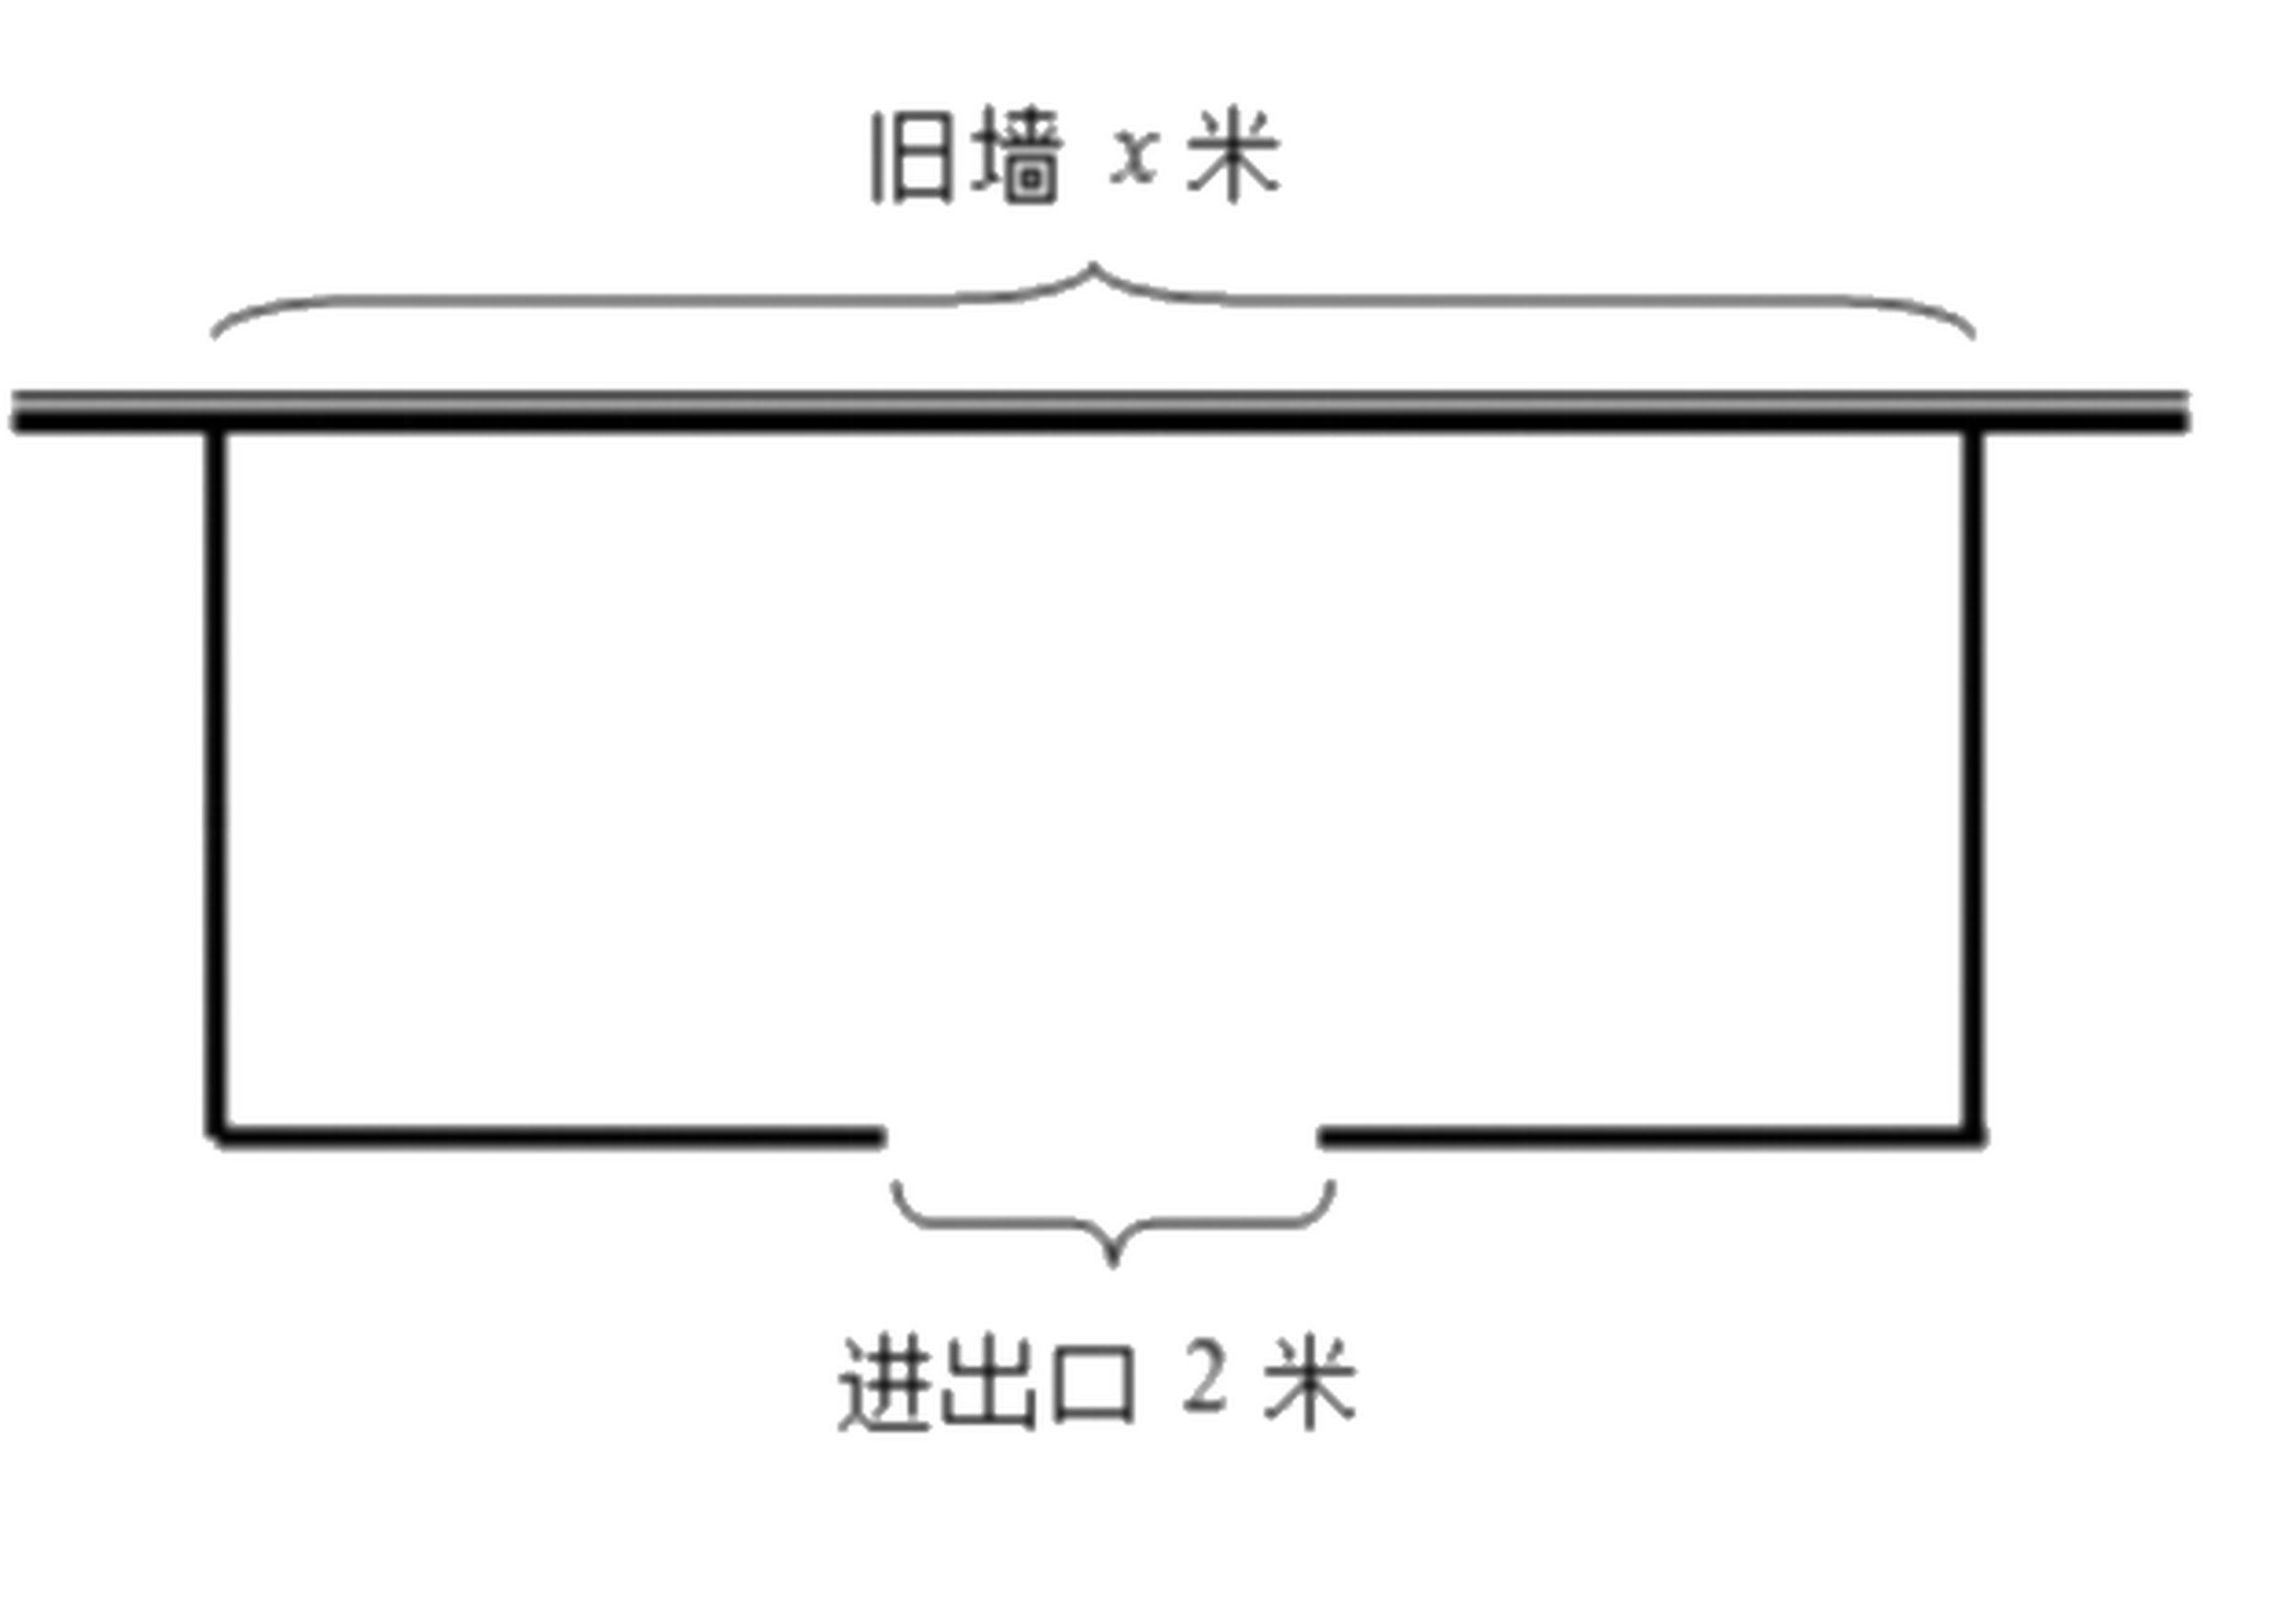
\includegraphics[width=0.60\textwidth]{figures/gao144_q17.png}
\end{center}

(1) 写出总费用 $y$ 关于 $x$ 的表达式;

(2) 试确定 $x$，使修建此矩形场地围墙的总费用最小，并求出最小总费用.

\ifanswer
\solbegin
\step{(1) 设矩形的另一边长为 $a$ 米，}
\step{则 $y=45x+180(x-2)+180\times2a=225x+360a-360$，}
\step{由已知 $xa=360$，得 $a=\dfrac{360}{x}$，所以 $y=225x+\dfrac{360^2}{x}-360(x>0)$;}
\step{(2) 因为 $x>0$，所以 $225x+\dfrac{360^2}{x}\geqslant2\sqrt{225x\cdot\dfrac{360^2}{x}}=10800$，}
\step{所以 $y=225x+\dfrac{360^2}{x}-360\geqslant10440$，}
\step{当且仅当 $225x=\dfrac{360^2}{x}$，即 $x=24$ 时取等号，}
\step{所以当 $x=24$ 米时，修建围墙的总费用最小，最小总费用是 10440 元.}
\solend
\fi

\item 已知集合 $A=\{a_1,a_2,\cdots,a_k\}(k\geqslant2)$，其中 $a_i\in\Z(i=1,2,\cdots,k)$. 定义：若对任意的 $x\in A$，必有 $-x\notin A$，则称集合 $A$ 具有性质 $G$. 由 $A$ 中元素可构成两个点集 $P$ 和 $Q$，$P=\{(x,y)\mid x\in A,y\in A,x+y\in A\}$，$Q=\{(x,y)\mid x\in A,y\in A,x-y\in A\}$，其中 $P$ 有 $m$ 个元素，$Q$ 中有 $n$ 个元素.

(1) 已知集合 $K=\{-1,2,3\}$，判断 $K$ 是否具有性质 $G$; 并写出 $K$ 对应的集合 $P$ 和集合 $Q$;

(2) 若集合 $A=\{1,2,3,4,5,6,7,8,9,10\}$，求对应集合 $Q$ 的元素个数; 一般地，若集合 $A$ 具有性质 $G$，且有 $k$ 个元素，猜测对应的集合 $Q$ 的元素最大个数，并说明理由;

(3) 若集合 $A$ 具有性质 $G$，猜测 $m,n$ 的大小并说明理由.

\ifanswer
\solbegin
\step{(1) 因为 $K=\{-1,2,3\},1,-2,-3$ 都不属于集合 $K$，}
\step{所以集合 $K$ 具有性质 $G$，}
\step{对应集合 $P=\{(-1,3),(3,-1)\},Q=\{(2,-1),(2,3)\}$;}
\step{(2) $A=\{1,2,3,4,5,6,7,8,9,10\}$，则对应集合 $Q$ 中的元素为:}
\step{$(2,1),(3,2),\cdots,(9,8),(10,9)$,}
\step{$(3,1),(4,2),\cdots,(9,7),(10,8)$,}
\step{$(4,1),(5,2),\cdots,(9,6),(10,7)$,}
\step{$\cdots$}
\step{$(9,1),(10,2)$,}
\step{$(10,1)$,}
\step{共有 $9+8+7+\cdots+2+1=45$ 个元素，即对应集合 $Q$ 的元素个数 45;}
\step{集合 $A$ 有 $k$ 个元素，猜测对应的集合 $Q$ 的最大个数为 $\dfrac{k^2-k}{2}$. 理由如下:}
\step{由题意得集合 $A$ 的元素构成有序数对 $(a_i,a_j)(i,j\in\N^*,i\leqslant k,j\leqslant k)$，}
\step{共有 $k^2$ 个，因为 $0\notin A$，所以 $(a_i,a_i)\notin Q$，}
\step{又因为 $a\in A$ 时，$-a\notin A$，所以 $(a_i,a_j)\in Q$ 时，$(a_j,a_i)\notin Q$，}
\step{所以集合 $Q$ 的元素个数为 $\dfrac{k^2-k}{2}$ 个，}
\step{(3) 当集合 $A$ 具有性质 $G$ 时，}
\step{①对于 $(a,b)\in P$，由定义得 $a\in A,b\in A,a+b\in A$，}
\step{又因为集合 $A$ 具有性质 $G$，所以 $(a+b,a)\in Q$，}
\step{如果 $(a,b),(c,d)$ 是 $P$ 中的不同元素，}
\step{那么 $a=c,b=d$ 中至少有一个不成立，}
\step{于是 $b=d,a+b=c+d$ 中至少有一个不成立，}
\step{故 $(a+b,b)$ 和 $(c+d,d)$ 也是 $Q$ 中不同的元素，}
\step{可见 $P$ 的元素个数不多于 $Q$ 的元素个数，即 $m\leqslant n$;}
\step{②对于 $(a,b)\in Q$，由定义得 $a\in A,b\in A,a-b\in A$，}
\step{又因为集合 $A$ 具有性质 $G$，则 $(a-b,b)\in P$，}
\step{如果 $(a,b),(c,d)$ 是 $Q$ 中的不同元素，}
\step{那么 $a=c,b=d$ 中至少有一个不成立，}
\step{于是 $b=d,a-b=c-d$ 中至少有一个不成立，}
\step{故 $(a-b,b)$ 和 $(c-d,d)$ 也是 $P$ 中不同的元素，}
\step{可见 $Q$ 的元素个数不多于 $P$ 的元素个数，即 $n\leqslant m$，}
\step{由①②得 $m=n$.}
\solend
\fi

\end{enumerate}

\end{document}
"
% 紧凑版：xelatex "\def\iscompact{1}% 高一144_风华中学_期中.tex
%   —— 高一上数学"2026-2027 年风华中学高一上期中"（试卷版/答案版/紧凑版）
% 试卷版：xelatex 高一144_风华中学_期中.tex
% 答案版：xelatex "\def\isanswer{1}\input{高一144_风华中学_期中.tex}"
% 紧凑版：xelatex "\def\iscompact{1}\input{高一144_风华中学_期中.tex}"
%
% ① 原始材料：微信公众号"魔都数学加油站"文章，连载"27学年高一144"，原文标题
% "27学年高一144——2026-2027年上海市风华中学高一上期中"；
% 原文链接：https://mp.weixin.qq.com/s/ylUlbXfudWOYC-jlH3jyjw 。
% 正文为 10 张 PNG 页，题目下印【解析】，为讲评版。
% 各页分辨率：01/02/03/05/06/07/09/10 为 2560×3620，04/08 为 4762×6735。
% 题目、解析均据原图转录；卷面粉红色水印"魔都数学加油站"及公众号页脚未录入。
% 全卷插图情况：Q17 有一幅矩形场地示意图（旧墙 x 米 / 进出口 2 米），从 07 页裁出、
%   去粉色水印去色 4× LANCZOS 放大存 figures/gao144_q17.png；其余 9 页逐页通读
%   确认无题目配图、无表格、亦无"题干写如图而源码漏图"一处。
%
% 卷首标题：原卷印作"2026-2027 年风华中学高一上期中"，年份区间按全稿惯例排 en dash；
% 原卷卷面未印副标题，本稿按同期中卷（高一140／141／143）知识模块口径补出
% "集合与常用逻辑用语、不等式、函数"：集合与逻辑见 Q3、Q7、Q9、Q10、Q12、Q16、Q18，
% 不等式见 Q6、Q11、Q13、Q14、Q15、Q17，函数见 Q4、Q5、Q8、Q9。
%
% 题号体例：本卷共 16 题——一、填空题 3—10（8 题）、二、选择题 11—13（3 题）、
% 三、解答题 14—18（5 题）。三节分别 \setcounter{enumi}{2}／{10}／{13}。
% 原卷从第 3 题起、无第 1、2 题，本稿保留原题号；全卷无附加题节。
%
% ② 与原卷的排版差异：
%   ① 原文从第 3 题起，本稿保留原题号；共 16 题三节；
%   ② 原卷 15 题题下印【解析】，唯 Q11 未印【解析】、只把答案"（ BD ）"直接印在
%      题干括号内（放大 04 页 A/B 选项与 05 页 C/D 选项衔接处确认，见 ⑤）；
%      按 高一128／94／106／140 成例：Q11 试卷版括号留空 \mbox{（\quad）}、
%      答案版另提 \ans{$BD$}、不补造原卷没有的解析；其余 15 题印【解析】、
%      括号内一律留空、不另提 \ans{}（Q12 选 C、Q13 选 B 在解析末句"故选 …"）；
%      答案版【答案】/【解析】标记数 = 16（1 个 \ans + 15 个 \solbegin）= 全卷题数；
%      正文 Q11 对应处另有 % 注；
%   ③ 原卷卷面未印副标题，本稿按知识模块口径补出；
%   ④ 原卷填空横线按全稿惯例排 \blankline[4.4em]；选择题括号排 \mbox{（\quad）}，
%      选项段前按惯例加 \keepwithprev；解答题不留作答区、不加 \anspace
%      （原卷为讲评版，与 129／131／132／133／136／140／141／143 同）；
%   ⑤ 数集：Q9 题干与解析"a,b∈R"、Q12 题干"U=R"、Q15 题干"x,y∈R"原卷印
%      斜体或黑板粗体 R，Q18 题干"a_i∈Z"印黑板粗体 Z、Q18 解析"i,j∈N*"印
%      黑板粗体 N，按全稿惯例统一改 \R／\Z／\N^*；绝对值排 \lvert…\rvert，
%      集合描述竖线排 \mid；不等号按全稿惯例排 \leqslant／\geqslant；
%      补集照原卷上划线排 \overline{A}／\overline{B}；空集记号 \varnothing；
%   ⑥ 子题标号 (1)(2)(3) 原卷印半角括号，照录；圈数字 ①② 在正文（文本模式）
%      按原卷照录（Q15、Q18 解析），未进数学式；数学式内半角逗号照录
%      （Q12 解析"$A=(1,2),B=(0,6)$"、Q18 解析"$(a_i,a_j)(i,j\in\N^*,i\leqslant k,j\leqslant k)$"、
%      Q15 解析"$x=1,y=-1$"、Q18 解析"$a=c,b=d$"等，为全稿惯例、非笔误）；
%      全卷行末西文句点照录为 ASCII `.`；行中全角逗号／顿号照录；
%      Q18 解析集合描述中的"或"用 \text{ 或 } 置于数学式内；
%   ⑦ 题干中的中文弯引号按原卷照录（Q3 的" x∈A "／" x∈B "与 Q15 (2) 的命题
%      引号，含引号内空格），注释内一律 ASCII 引号；
%   ⑧ Q17 配图：题干写"如图所示"，配图居中排在题干之后、子问之前，三版都出；
%      在 Q17 \item 之前加 \needvspace{10cm} 把"题干＋图"整块推走。Q17 是
%      "三、解答题"节内第 4 题（非节首题），故守卫放在 \item 之前而非 \bigsec
%      之前不会让节标题孤落页末（B 类）；三版切页审计均"合计异常：无"；
%   ⑨ 跨页续印按题合并：Q3 在 01 页；Q4/5/6 在 01 页（Q6 解析续到 02 页顶）；
%      Q7/8/9 在 02 页（Q9 题干跨 02→03）；Q10 在 03 页、解析跨 03→04（很长，
%      按余数分组 A₁/A₂/A₃）；Q11 在 04 页（"二、选择题"节标题也在 04 页下部）、
%      Q12/13 在 05 页（"三、解答题"标题在 05 页下部）；Q14 在 05 页末、解析在 06 页；
%      Q15/16 在 06 页（Q16 续到 07 页）；Q17 在 07 页；Q18 在 08 页、解析跨
%      08/09/10 页（性质 G 压轴，3 问，很长）；本稿按题连排，不丢行、不并折行；
%   ⑩ Q8 解析"法一：""法二："两处标签经放大 02 页逐字确认原卷均印红色
%      （见 ⑤）；按全稿惯例（高一53 成例）不引入红色、均照录为黑体着色
%      \stepm{法一：}{…}／\stepm{法二：}{…}，不改 common.sty；
%      文件头在此注明原卷为红色；
%   ⑪ "图像／图象"逐处核：全卷未出现"图像"或"图象"字样，无统一问题；
%   ⑫ \left…\right 不得拆到不同 $…$ 组；cases 块整体算一个印刷行；
%      Q4 分式与 8×(-3/4) 同一 $…$ 组，Q13 的 \left(\frac1x+\frac2y\right) 同理。
%
% ③ 行数复核：一条 \step／\stepm 行 = 原卷解析的一个印刷行，cases 块作一个印刷行计。
%   逐题数（含 \stepm）：Q3：3；Q4：1；Q5：1；Q6：5；Q7：4；Q8：8（6 \step
%   ＋ 2 \stepm，法一/法二标签各占 1 行）；Q9：6；Q10：23；Q11：0（原卷无解析，
%   答案另提 \ans{$BD$}）；Q12：5；Q13：3；Q14：5；Q15：8；Q16：7；Q17：7；
%   Q18：32。合计 116 条 \step ＋ 2 条 \stepm ＝ 118 个印刷行，与原卷逐题相等。
%   全卷 15 题设 \solbegin…\solend ＋ Q11 一处 \ans{}，答案版【答案】/【解析】
%   标记数 = 16 = 全卷题数。
%
% ④ 判别式／子集符号结论（逐处放大原图照录、不得统一）：
%   判别式全卷 2 处，逐页放大扫过 10 页确认（Q4 为分式指数化简、不含判别式）：
%     · Q9【解析】"所以 △=a^2-4b=0" 原卷印细线、扁等边三角（宽≈高、笔画细，
%       放大见 /tmp/gao144fh/z_q9_tri.png、z_tri_Q9.png），照录 \triangle；
%     · Q15 (2)【解析】cases 块"Δ=(a-2)^2-4(a-2)≤0" 原卷印等腰偏高、粗笔画
%       三角（高>宽，放大见 z_q15_tri.png、z_tri_Q15.png），照录 \Delta；
%   两形不同、全卷混用，逐处照录不统一（参照 高一142 头注④口径）。
%   子集符号全卷 4 处，逐处放大核：
%     · Q3 解析"所以 B⊆A"、Q16 (1) 解析"所以 B⊆A" 原卷均印带下划线的 ⊆
%       （z_q3_symbol.png、z_q16_subset2.png），照录 \subseteq；
%     · Q12 选项 B"$\overline{A}\subset B$" 原卷印单线 ⊂（z_q12_opts2.png），
%       照录 \subset；Q12 解析"$\overline{A}=(-\infty,1]\cup[2,+\infty)\not\subset B$"
%       原卷印单线带斜杠 ⊄（z_q12_notsym3.png），照录 \not\subset；
%   \subset 与 \subseteq 混用，逐处照录不统一。补集照原卷上划线 \overline{A}／
%   \overline{B}，空集 \varnothing，数集 \R／\Z／\N^* 归一见 ② ⑤。
%
% ⑤ 存疑／特殊体例（主会话逐处放大原图复核确认，照录未改，正文对应处另有 % 注）：
%   1. 第 11 题原卷把答案"（ BD ）"直接印在题干括号内、题下未印【解析】
%      （放大 04 页 A/B 选项与 05 页 C/D 选项衔接处确认：05 页顶 C/D 选项后
%      直接接第 12 题）。按 高一128／94／106／140 成例括号留空、另提
%      \ans{$BD$}，不补造解析（不编造）。
%   2. 第 10 题题干"集合 $S$ 为集合 $M=\{1,2,3,4,\cdots,2026\}$，的子集"在
%      集括号与"的子集"之间原卷多印一个全角逗号（放大 03 页确认），
%      按存疑照录未删，正文对应处另有 % 注。
%   3. 第 8 题解析"法一：""法二："两处原卷均印红色（放大 02 页逐字确认），
%      按全稿惯例不引入红色、两处均照录为黑体着色 \stepm（见 ② ⑩）。
%   全卷除此 3 条外未发现其它笔误／自相矛盾处。
%
% ⑥ 跨页续印按题合并说明：见 ② ⑨。
%
\documentclass[a4paper,11pt]{article}
\usepackage{common}

\begin{document}

\examtitlest[3]{2026--2027 年风华中学高一上期中}{集合与常用逻辑用语、不等式、函数}

\bigsec{一、填空题}

\begin{enumerate}
\setcounter{enumi}{2}

\item $A=\{x\mid x>4\}$，$B=\{x\mid x>a\}$，若命题 “ $x\in A$ ” 是命题 “ $x\in B$ ” 的必要条件，则 $a$ 的取值范围是\blankline[4.4em].

\ifanswer
\solbegin
\step{因为 “ $x\in A$ ” 是命题 “ $x\in B$ ” 的必要条件，所以 $B\subseteq A$，}% 子集符号原卷印带下划线 $\subseteq$，照录
\step{因为 $A=\{x\mid x>4\}$，$B=\{x\mid x>a\}$，所以 $a\geqslant4$，}
\step{所以 $a$ 的取值范围是 $\{a\mid a\geqslant4\}$.}
\solend
\fi

\item 已知 $a>0,b>0$，化简式子：$\dfrac{8a^{\frac34}b^3}{\left(a^{\frac16}b^{\frac32}\right)\left(-\dfrac43 a^{\frac1{12}}b^{\frac12}\right)}=$\blankline[4.4em].

\ifanswer
\solbegin
\step{$\dfrac{8a^{\frac34}b^3}{\left(a^{\frac16}b^{\frac32}\right)\left(-\dfrac43 a^{\frac1{12}}b^{\frac12}\right)}=8\times\left(-\dfrac34\right)a^{\frac34-\frac16-\frac1{12}}b^{3-\frac32-\frac12}=-6a^{\frac12}b=-6b\sqrt a$.}
\solend
\fi

\item 已知 $\lg2=a$，$\lg3=b$，则 $\log_5 6=$\blankline[4.4em]（结果用 $a,b$ 表示）.

\ifanswer
\solbegin
\step{$\log_5 6=\dfrac{\lg6}{\lg5}=\dfrac{\lg2+\lg3}{1-\lg2}=\dfrac{a+b}{1-a}$.}
\solend
\fi

\item 若关于 $x$ 的不等式 $ax>b$ 的解集为 $(-\infty,2)$，则不等式 $bx+a>0$ 的解集为\blankline[4.4em].

\ifanswer
\solbegin
\step{因为不等式 $ax>b$ 的解集为 $(-\infty,2)$，所以 $a<0$，}
\step{所以由不等式解得 $x<\dfrac ba$，所以 $\dfrac ba=2$，即 $b=2a$，}
\step{代入不等式 $bx+a>0$，得 $2ax+a>0$，}
\step{因为 $a<0$，所以不等式化为 $2x+1<0$，解得 $x<-\dfrac12$，}
\step{故不等式的解集为 $\left(-\infty,-\dfrac12\right)$.}
\solend
\fi

\item 如果集合 $A=\{x\mid x^2-4x\leqslant0\}$，$B=\{x\mid x^2+ax+b\leqslant0\}$，$A\cap B=\{x\mid3\leqslant x\leqslant4\}$，$A\cup B=\{x\mid0\leqslant x\leqslant5\}$，则 $a+b=$\blankline[4.4em].

\ifanswer
\solbegin
\step{由题意得 $A=\{x\mid x^2-4x\leqslant0\}=[0,4]$，}
\step{又因为 $A\cap B=\{x\mid3\leqslant x\leqslant4\}$，$A\cup B=\{x\mid0\leqslant x\leqslant5\}$，}
\step{所以 $B=\{x\mid3\leqslant x\leqslant5\}$，即方程 $x^2+ax+b=0$ 的两根为 $3,5$，}
\step{由韦达定理得 $\begin{cases}3+5=-a\\3\times5=b\end{cases}$，解得 $a=-8$，$b=15$，所以 $a+b=15-8=7$.}
\solend
\fi

% 第 8 题：原卷"法一：""法二："两处标签均印红色（8× 放大确认）；按交办口径
% "法一"用普通 \step、"法二："排 \stepm（加粗着色、不引红色），见头注 ② ⑩／⑤
\item 若关于 $x$ 的方程 $\lvert x-1\rvert+\lvert\pi-x\rvert=\pi-1$ 的解集为\blankline[4.4em].

\ifanswer
\solbegin
\stepm{法一：}{因为 $\lvert x-1\rvert+\lvert\pi-x\rvert=\begin{cases}x-1+x-\pi,x\geqslant\pi\\\pi-1,1<x<\pi\\1-x+\pi-x,x\leqslant1\end{cases}=\begin{cases}2x-1-\pi,x\geqslant\pi\\\pi-1,1<x<\pi\\1+\pi-2x,x\leqslant1\end{cases}$.}
\step{当 $x\geqslant\pi$ 时，令 $2x-1-\pi=\pi-1$，得 $x=\pi$；}
\step{当 $1<x<\pi$ 时，$\lvert x-1\rvert+\lvert\pi-x\rvert=\pi-1$ 恒成立；}
\step{当 $x\leqslant1$ 时，令 $1+\pi-2x=\pi-1$，得 $x=1$.}
\step{综上所述，方程 $\lvert x-1\rvert+\lvert\pi-x\rvert=\pi-1$ 的解集为 $[1,\pi]$.}
\stepm{法二：}{因为 $\lvert x-1\rvert+\lvert\pi-x\rvert\geqslant\lvert x-1+\pi-x\rvert=\pi-1$，}
\step{当且仅当 $(x-1)(\pi-x)\geqslant0$ 时取等号，}
\step{故方程 $\lvert x-1\rvert+\lvert\pi-x\rvert=\pi-1$ 的解集为 $[1,\pi]$.}
\solend
\fi

% 第 9 题：题干跨 02→03 页；解析判别式原卷印细线扁等边三角 $\triangle$，照录
\item 已知函数 $f(x)=x^2+ax+b(a,b\in\R)$ 和 $x$ 轴有且只有一个交点，若关于 $x$ 的不等式 $f(x)<c$ 的解集为 $(m,m+6)$，则 $c=$\blankline[4.4em].

\ifanswer
\solbegin
\step{因为函数 $f(x)=x^2+ax+b(a,b\in\R)$ 和 $x$ 轴有且只有一个交点，}
\step{所以 $\triangle=a^2-4b=0$，即 $b=\dfrac{a^2}{4}$，}% 判别式原卷印扁等边三角 $\triangle$，照录
\step{不等式 $f(x)<c$ 的解集为 $(m,m+6)$，}
\step{即 $x^2+ax+\dfrac{a^2}{4}-c<0$ 的解集为 $(m,m+6)$，}
\step{所以方程 $x^2+ax+\dfrac{a^2}{4}-c=0$ 的两个根为 $x_1=m$，$x_2=m+6$，}
\step{所以 $\begin{cases}x_1+x_2=2m+6=-a\\x_1x_2=m(m+6)=\dfrac{a^2}{4}-c\end{cases}$，消去 $m$ 得 $\dfrac{a^2}{4}-9=\dfrac{a^2}{4}-c$，解得 $c=9$.}
\solend
\fi

% 第 10 题：原卷题干在集括号与"的子集"之间多印一个全角逗号，照录未改（存疑，见头注 ⑤）
\item 已知集合 $S$ 为集合 $M=\{1,2,3,4,\cdots,2026\}$，的子集，并且集合 $S$ 中任意两个元素之和不能被 3 整除，则集合 $S$ 中元素个数的最大值为\blankline[4.4em].

\ifanswer
\solbegin
\step{对于集合 $M=\{1,2,3,4,\cdots,2026\}$，}
\step{所有被 3 除余数为 0 的元素组成的集合为 $A_3=\{3,6,9,\cdots,2025\}$，}
\step{元素个数为 675;}
\step{所有被 3 除余数为 1 的元素组成的集合为 $A_1=\{1,4,7,\cdots,2026\}$，}
\step{元素个数为 676;}
\step{所有被 3 除余数为 2 的元素组成的集合为 $A_2=\{2,5,8,\cdots,2024\}$，}
\step{元素个数为 675;}
\step{集合 $S$ 中任意两个元素之和不能被 3 整除，}
\step{若两个元素分别来自 $A_1$ 和 $A_2$，则两数之和除以 3 的余数为 $1+2=3\equiv0$，}
\step{即和能被 3 整除，}
\step{所以 $S$ 不能同时包含 $A_1$ 和 $A_2$ 中的元素，}
\step{即 $S$ 最多只能选取 $A_1$、$A_2$ 一个集合中的全部元素;}
\step{若两个元素都来自 $A_3$，则两数之和除以 3 的余数为 $0+0=0$，即和能被 3 整除，}
\step{所以 $S$ 中最多包含 $A_3$ 中的 1 个元素;}
\step{对 $A_1$ 内的任意两个元素，其和除以 3 的余数为 $1+1=2$，不能被 3 整除;}
\step{$A_1$ 中元素与 $A_3$ 中元素的和除以 3 余数为 $1+0=1$，不能被 3 整除，}
\step{所以 $A_1$ 的全部元素与 $A_3$ 中的任意 1 个元素的组合满足题意;}
\step{对 $A_2$ 内的任意两个元素，其和除以 3 的余数为 $2+2=4\equiv1$，不能被 3 整除;}
\step{$A_2$ 中元素与 $A_3$ 中元素的和除以 3 的余数为 $2+0=2$，不能被 3 整除，}
\step{所以 $A_2$ 的全部元素与 $A_3$ 中任意 1 个元素的组合也满足题意.}
\step{故若选取 $A_2$ 全部元素加 1 个 $A_3$ 元素，总个数为 $675+1=676$;}
\step{选取 $A_1$ 全部元素加 1 个 $A_3$ 元素，总个数为 $676+1=677$;}
\step{所以集合 $S$ 中元素个数的最大值为 677.}
\solend
\fi

\end{enumerate}

\bigsec{二、选择题}

\begin{enumerate}
\setcounter{enumi}{10}

% 第 11 题：原卷把答案"（ BD ）"直接印在题干括号内、题下无【解析】（放大 04 页 A/B 选项
% 与 05 页 C/D 选项衔接处确认）。按 高一128／94／106／140 成例：试卷版括号留空、
% 答案版另提 \ans{$BD$}、不补造原卷没有的解析（不编造）。
\item 已知实数 $a,b$，下列四个不等式中正确的是\mbox{（\quad）}

\keepwithprev
A. $a+\dfrac1a\geqslant2$\qquad B. $\sqrt{a^2+2}+\dfrac{1}{\sqrt{a^2+2}}\geqslant2$

C. $\dfrac{a+b}{2}\leqslant\sqrt{ab}$\qquad D. $a^2+b^2\geqslant2ab$

\ifanswer
\ans{$BD$}
\fi

\item 若全集 $U=\R$，$A=\{x\mid x^2-3x+2<0\}$，$B=\{x\mid0<x<6\}$，则\mbox{（\quad）}

\keepwithprev
A. $A\cap B=B$\qquad B. $\overline{A}\subset B$\qquad C. $A\cap\overline{B}=\varnothing$\qquad D. $A\cup B=A$

\ifanswer
\solbegin
\step{由 $x^2-3x+2<0$，则 $A=(1,2),B=(0,6)$，所以 $A\cap B=(1,2)=A,A$ 错误;}
\step{$\overline{A}=(-\infty,1]\cup[2,+\infty)\not\subset B$，$B$ 错误;}
\step{$\overline{B}=(-\infty,0]\cup[6,+\infty)$，所以 $A\cap\overline{B}=\varnothing,C$ 正确;}
\step{$A\cup B=(0,6)\ne A,D$ 错误.}
\step{故选 $C$.}
\solend
\fi

\item 已知正数 $x$、$y$ 满足 $\dfrac1x+\dfrac2y=1$，不等式 $3x+2y-1>m$ 恒成立，则实数 $m$ 的取值范围是\mbox{（\quad）}

\keepwithprev
A. $(-\infty,4+6\sqrt2)$\qquad B. $(-\infty,6+4\sqrt3)$\qquad C. $(6+4\sqrt2,+\infty)$\qquad D. $(8+4\sqrt3,+\infty)$

\ifanswer
\solbegin
\step{$3x+2y=(3x+2y)\left(\dfrac1x+\dfrac2y\right)=7+\dfrac{6x}{y}+\dfrac{2y}{x}\geqslant7+2\sqrt{\dfrac{6x}{y}\cdot\dfrac{2y}{x}}=7+4\sqrt3$，}
\step{当且仅当 $\dfrac{6x}{y}=\dfrac{2y}{x}$，即 $y=\sqrt3x=\sqrt3+2$ 时取等号，}
\step{故要使原式成立，只需 $m<6+4\sqrt3$. 故选 $B$.}
\solend
\fi

\end{enumerate}

\bigsec{三、解答题}

\begin{enumerate}
\setcounter{enumi}{13}

\item 解关于 $x$ 的不等式：

(1) $x^2-2\lvert x\rvert-3>0$；

(2) $\dfrac{2x-1}{x+2}<1$.

\ifanswer
\solbegin
\step{(1) 原不等式等价于 $(\lvert x\rvert-3)(\lvert x\rvert+1)>0$，}
\step{$\lvert x\rvert+1>0$，故 $\lvert x\rvert>3$，解得 $x<-3$ 或 $x>3$，}
\step{故不等式的解集为 $(-\infty,-3)\cup(3,+\infty)$.}
\step{(2) 已知 $\dfrac{2x-1}{x+2}<1$，则 $\dfrac{2x-1}{x+2}-1<0$，即 $\dfrac{x-3}{x+2}<0$，}
\step{等价于 $(x-3)(x+2)<0$，解得 $-2<x<3$，故不等式的解集为 $(-2,3)$.}
\solend
\fi

\item (1) 已知 $x,y\in\R$，比较 $x^2+y^2$ 与 $2x-2y-2$ 的大小.

(2) “不等式 $(a-2)x^2+(a-2)x+1\geqslant0$ 对一切实数恒成立” 是假命题，求实数 $a$ 的取值范围.

\ifanswer
\solbegin
\step{(1) $x^2+y^2-(2x-2y-2)=x^2+y^2-2x+2y+2=(x-1)^2+(y+1)^2\geqslant0$，}
\step{故 $x^2+y^2\geqslant2x-2y-2$，当且仅当 $x=1,y=-1$ 时取等号.}
\step{(2) 先求命题 “$(a-2)x^2+(a-2)x+1\geqslant0$ 对一切实数恒成立” 为真，}
\step{①当 $a-2=0$ 时，即 $a=2$，不等式化为 $1\geqslant0$，成立，符合条件，}
\step{②当 $a-2\ne0$ 时，则 $\begin{cases}a-2>0\\\Delta=(a-2)^2-4(a-2)\leqslant0\end{cases}$，解得 $2<a\leqslant6$，}% 判别式原卷印等腰偏高三角 $\Delta$，照录
\step{综上①②，命题为真时 $2\leqslant a\leqslant6$，}
\step{该命题为假命题，则 $a<2$ 或 $a>6$，}
\step{所以实数 $a$ 的取值范围是 $(-\infty,2)\cup(6,+\infty)$.}
\solend
\fi

\item 设集合 $A=\{x\mid-1\leqslant x\leqslant2\}$，$B=\{x\mid m-1<x<2m+1\}$.

(1) 若 $A\cup B=A$，求实数 $m$ 的取值范围;

(2) 若 $B\cap\overline{A}$ 中只有一个整数 $-2$，求实数 $m$ 的取值范围.

\ifanswer
\solbegin
\step{(1) 因为 $A\cup B=A$，所以 $B\subseteq A$，}% 子集符号原卷印带下划线 $\subseteq$，照录
\step{当 $B=\varnothing$ 时，有 $m-1\geqslant2m+1$，解得 $m\leqslant-2$；}
\step{当 $B\ne\varnothing$ 时，有 $\begin{cases}m-1<2m+1\\m-1\geqslant-1\\2m+1\leqslant2\end{cases}$，解得 $0\leqslant m\leqslant\dfrac12$，}
\step{所以实数 $m$ 的取值范围是 $(-\infty,-2]\cup\left[0,\dfrac12\right]$;}
\step{(2) 由集合 $A=\{x\mid-1\leqslant x\leqslant2\}$，得 $\overline{A}=\{x\mid x<-1\text{ 或 }x>2\}$，}
\step{若 $B\cap\overline{A}$ 中只有一个整数 $-2$，则 $B\ne\varnothing$，且满足 $\begin{cases}m-1<2m+1\\-3\leqslant m-1<-2\\-2<2m+1\leqslant3\end{cases}$}
\step{解得 $-\dfrac32<m<-1$，所以实数 $m$ 的取值范围是 $\left(-\dfrac32,-1\right)$.}
\solend
\fi

% 第 17 题配图是"题干＋图"整块；守卫放在 \item 之前（Q17 非节首题，不会让节标题孤落页末）
\needvspace{10cm}
\item 现要围建一个面积为 360 平方米的矩形场地，要求矩形场地的一面利用旧墙（利用旧墙需维修），其它三面围墙要新建，在旧墙的对面的新墙上要留一个宽度为 2 米的进出口，如图所示，已知旧墙的维修费用为 45 元/米，新墙的造价为 180 元/米，设利用的旧墙的长度为 $x$ 米，工程总造价为 $y$（单位：元）.

\begin{center}
% 矩形场地示意图取自 07 页右侧，去粉色水印、去色、4× LANCZOS 放大
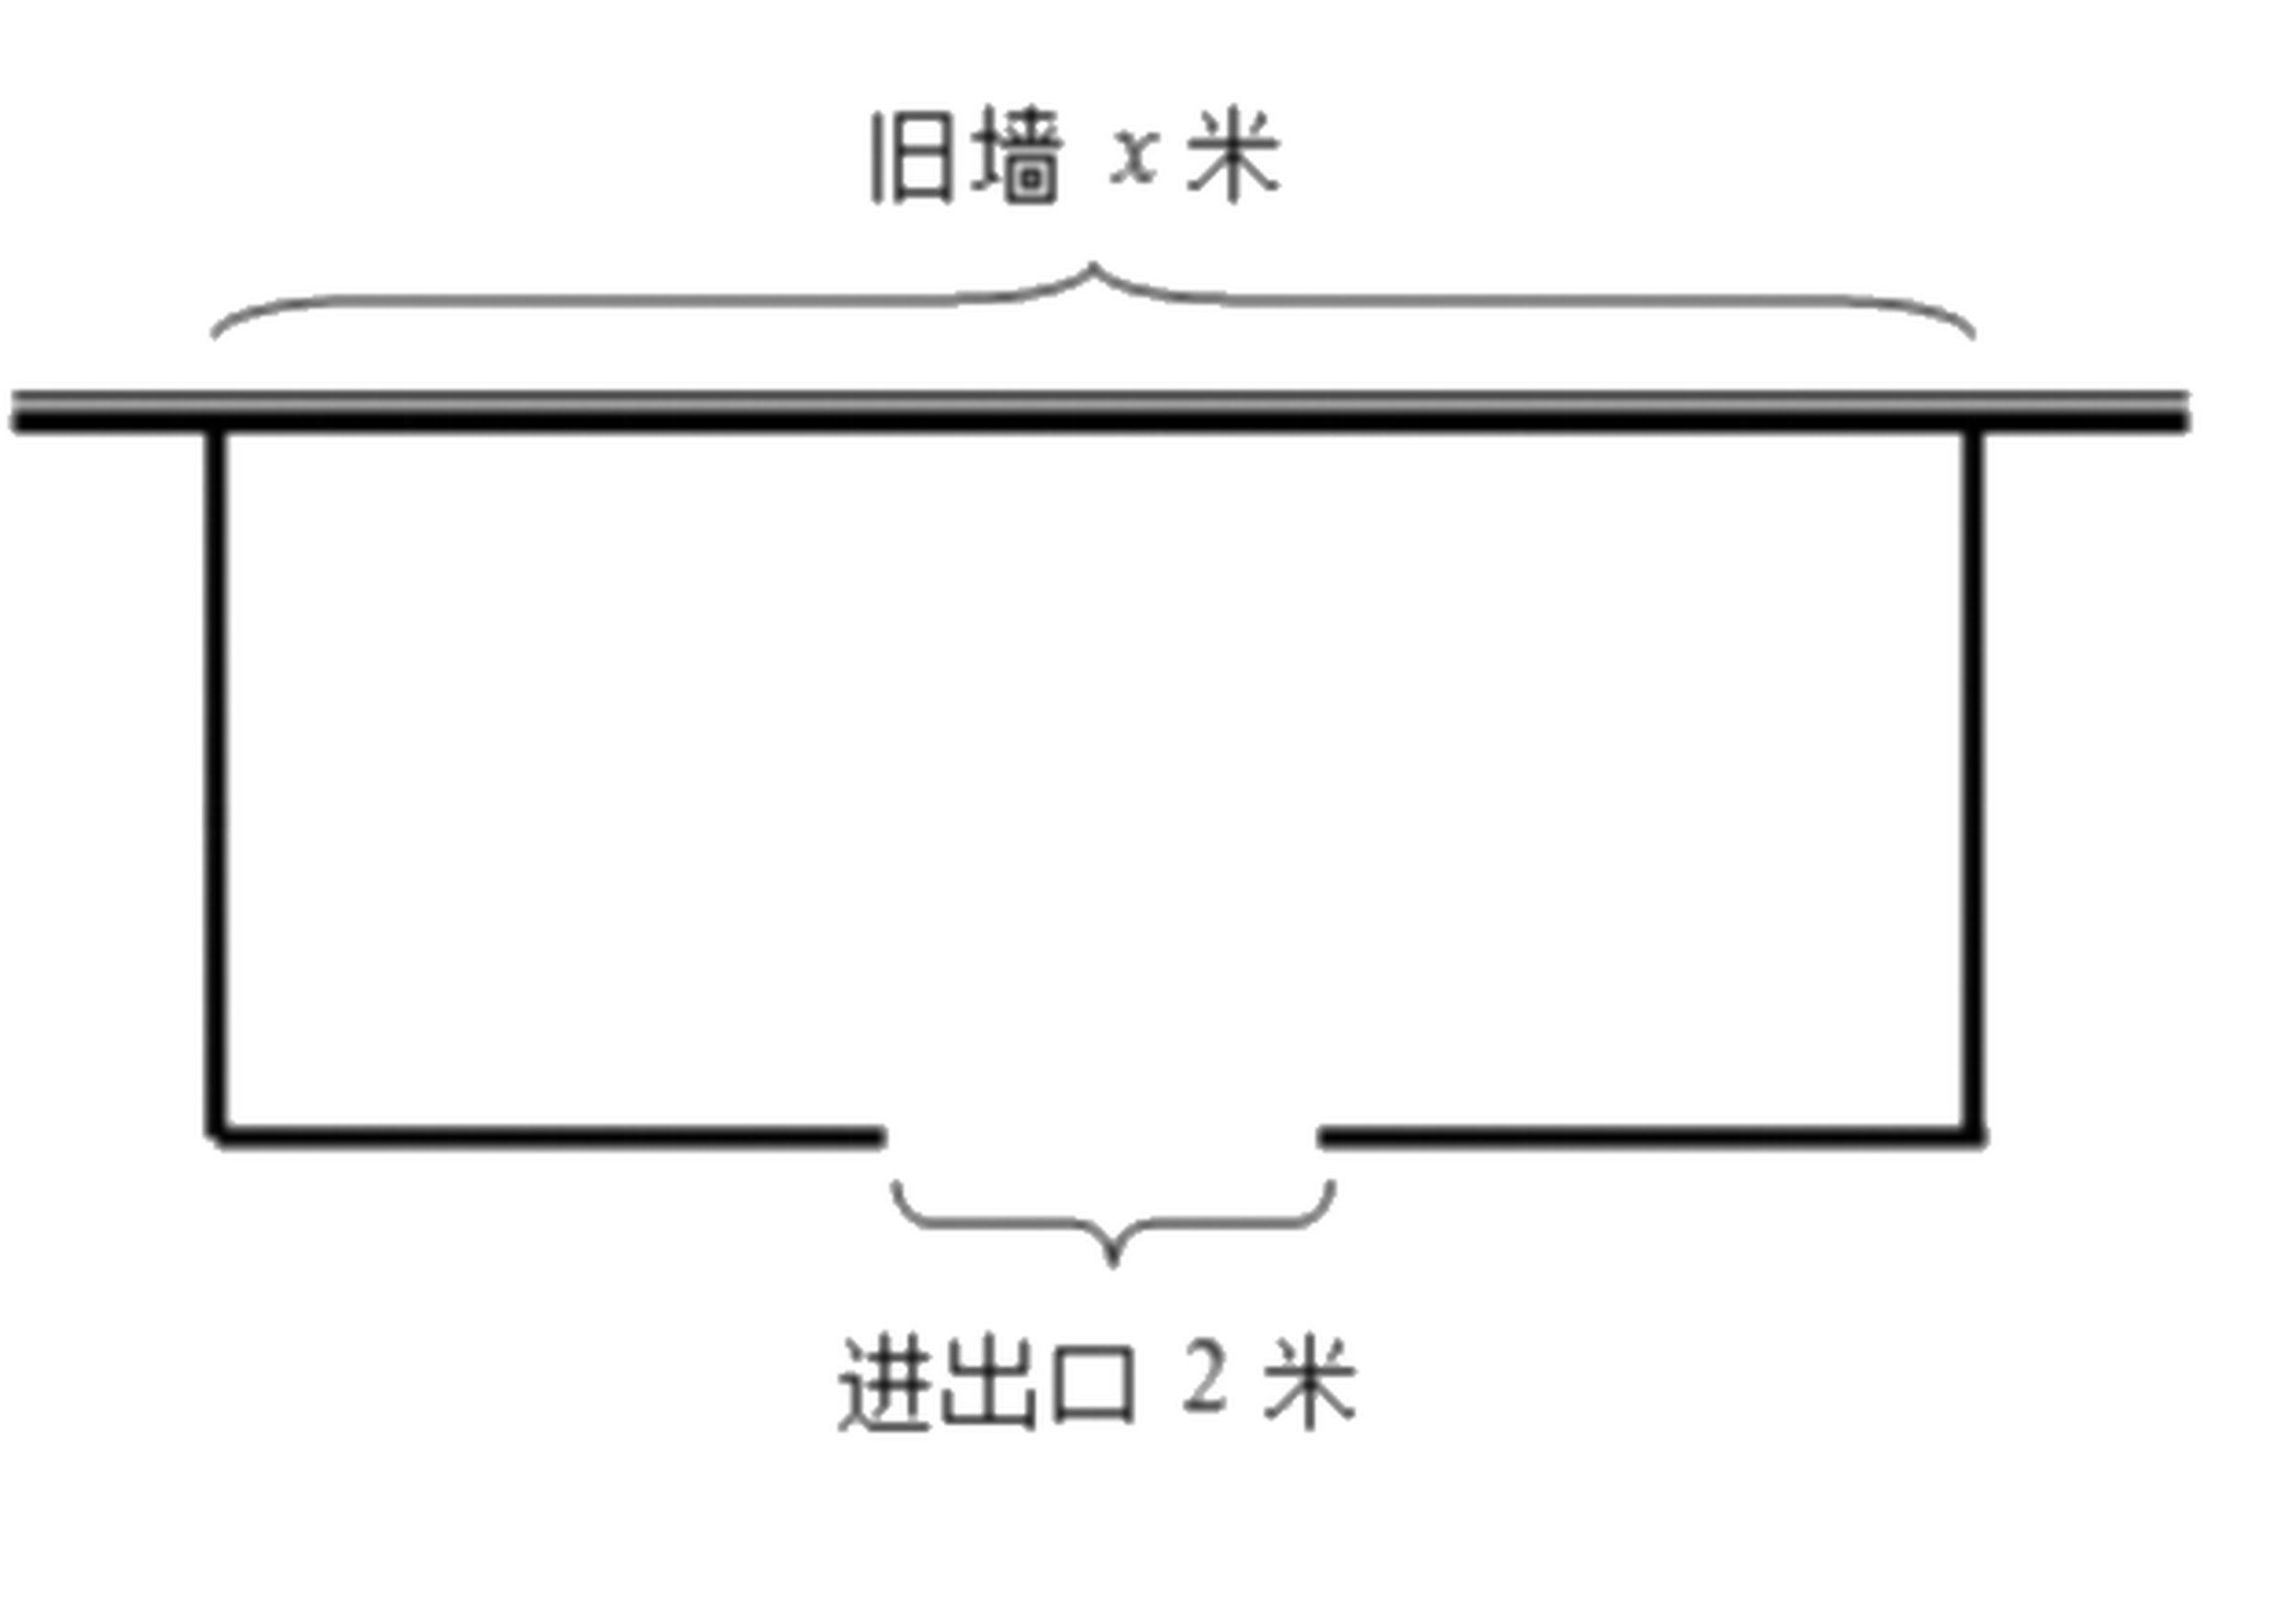
\includegraphics[width=0.60\textwidth]{figures/gao144_q17.png}
\end{center}

(1) 写出总费用 $y$ 关于 $x$ 的表达式;

(2) 试确定 $x$，使修建此矩形场地围墙的总费用最小，并求出最小总费用.

\ifanswer
\solbegin
\step{(1) 设矩形的另一边长为 $a$ 米，}
\step{则 $y=45x+180(x-2)+180\times2a=225x+360a-360$，}
\step{由已知 $xa=360$，得 $a=\dfrac{360}{x}$，所以 $y=225x+\dfrac{360^2}{x}-360(x>0)$;}
\step{(2) 因为 $x>0$，所以 $225x+\dfrac{360^2}{x}\geqslant2\sqrt{225x\cdot\dfrac{360^2}{x}}=10800$，}
\step{所以 $y=225x+\dfrac{360^2}{x}-360\geqslant10440$，}
\step{当且仅当 $225x=\dfrac{360^2}{x}$，即 $x=24$ 时取等号，}
\step{所以当 $x=24$ 米时，修建围墙的总费用最小，最小总费用是 10440 元.}
\solend
\fi

\item 已知集合 $A=\{a_1,a_2,\cdots,a_k\}(k\geqslant2)$，其中 $a_i\in\Z(i=1,2,\cdots,k)$. 定义：若对任意的 $x\in A$，必有 $-x\notin A$，则称集合 $A$ 具有性质 $G$. 由 $A$ 中元素可构成两个点集 $P$ 和 $Q$，$P=\{(x,y)\mid x\in A,y\in A,x+y\in A\}$，$Q=\{(x,y)\mid x\in A,y\in A,x-y\in A\}$，其中 $P$ 有 $m$ 个元素，$Q$ 中有 $n$ 个元素.

(1) 已知集合 $K=\{-1,2,3\}$，判断 $K$ 是否具有性质 $G$; 并写出 $K$ 对应的集合 $P$ 和集合 $Q$;

(2) 若集合 $A=\{1,2,3,4,5,6,7,8,9,10\}$，求对应集合 $Q$ 的元素个数; 一般地，若集合 $A$ 具有性质 $G$，且有 $k$ 个元素，猜测对应的集合 $Q$ 的元素最大个数，并说明理由;

(3) 若集合 $A$ 具有性质 $G$，猜测 $m,n$ 的大小并说明理由.

\ifanswer
\solbegin
\step{(1) 因为 $K=\{-1,2,3\},1,-2,-3$ 都不属于集合 $K$，}
\step{所以集合 $K$ 具有性质 $G$，}
\step{对应集合 $P=\{(-1,3),(3,-1)\},Q=\{(2,-1),(2,3)\}$;}
\step{(2) $A=\{1,2,3,4,5,6,7,8,9,10\}$，则对应集合 $Q$ 中的元素为:}
\step{$(2,1),(3,2),\cdots,(9,8),(10,9)$,}
\step{$(3,1),(4,2),\cdots,(9,7),(10,8)$,}
\step{$(4,1),(5,2),\cdots,(9,6),(10,7)$,}
\step{$\cdots$}
\step{$(9,1),(10,2)$,}
\step{$(10,1)$,}
\step{共有 $9+8+7+\cdots+2+1=45$ 个元素，即对应集合 $Q$ 的元素个数 45;}
\step{集合 $A$ 有 $k$ 个元素，猜测对应的集合 $Q$ 的最大个数为 $\dfrac{k^2-k}{2}$. 理由如下:}
\step{由题意得集合 $A$ 的元素构成有序数对 $(a_i,a_j)(i,j\in\N^*,i\leqslant k,j\leqslant k)$，}
\step{共有 $k^2$ 个，因为 $0\notin A$，所以 $(a_i,a_i)\notin Q$，}
\step{又因为 $a\in A$ 时，$-a\notin A$，所以 $(a_i,a_j)\in Q$ 时，$(a_j,a_i)\notin Q$，}
\step{所以集合 $Q$ 的元素个数为 $\dfrac{k^2-k}{2}$ 个，}
\step{(3) 当集合 $A$ 具有性质 $G$ 时，}
\step{①对于 $(a,b)\in P$，由定义得 $a\in A,b\in A,a+b\in A$，}
\step{又因为集合 $A$ 具有性质 $G$，所以 $(a+b,a)\in Q$，}
\step{如果 $(a,b),(c,d)$ 是 $P$ 中的不同元素，}
\step{那么 $a=c,b=d$ 中至少有一个不成立，}
\step{于是 $b=d,a+b=c+d$ 中至少有一个不成立，}
\step{故 $(a+b,b)$ 和 $(c+d,d)$ 也是 $Q$ 中不同的元素，}
\step{可见 $P$ 的元素个数不多于 $Q$ 的元素个数，即 $m\leqslant n$;}
\step{②对于 $(a,b)\in Q$，由定义得 $a\in A,b\in A,a-b\in A$，}
\step{又因为集合 $A$ 具有性质 $G$，则 $(a-b,b)\in P$，}
\step{如果 $(a,b),(c,d)$ 是 $Q$ 中的不同元素，}
\step{那么 $a=c,b=d$ 中至少有一个不成立，}
\step{于是 $b=d,a-b=c-d$ 中至少有一个不成立，}
\step{故 $(a-b,b)$ 和 $(c-d,d)$ 也是 $P$ 中不同的元素，}
\step{可见 $Q$ 的元素个数不多于 $P$ 的元素个数，即 $n\leqslant m$，}
\step{由①②得 $m=n$.}
\solend
\fi

\end{enumerate}

\end{document}
"
%
% ① 原始材料：微信公众号"魔都数学加油站"文章，连载"27学年高一144"，原文标题
% "27学年高一144——2026-2027年上海市风华中学高一上期中"；
% 原文链接：https://mp.weixin.qq.com/s/ylUlbXfudWOYC-jlH3jyjw 。
% 正文为 10 张 PNG 页，题目下印【解析】，为讲评版。
% 各页分辨率：01/02/03/05/06/07/09/10 为 2560×3620，04/08 为 4762×6735。
% 题目、解析均据原图转录；卷面粉红色水印"魔都数学加油站"及公众号页脚未录入。
% 全卷插图情况：Q17 有一幅矩形场地示意图（旧墙 x 米 / 进出口 2 米），从 07 页裁出、
%   去粉色水印去色 4× LANCZOS 放大存 figures/gao144_q17.png；其余 9 页逐页通读
%   确认无题目配图、无表格、亦无"题干写如图而源码漏图"一处。
%
% 卷首标题：原卷印作"2026-2027 年风华中学高一上期中"，年份区间按全稿惯例排 en dash；
% 原卷卷面未印副标题，本稿按同期中卷（高一140／141／143）知识模块口径补出
% "集合与常用逻辑用语、不等式、函数"：集合与逻辑见 Q3、Q7、Q9、Q10、Q12、Q16、Q18，
% 不等式见 Q6、Q11、Q13、Q14、Q15、Q17，函数见 Q4、Q5、Q8、Q9。
%
% 题号体例：本卷共 16 题——一、填空题 3—10（8 题）、二、选择题 11—13（3 题）、
% 三、解答题 14—18（5 题）。三节分别 \setcounter{enumi}{2}／{10}／{13}。
% 原卷从第 3 题起、无第 1、2 题，本稿保留原题号；全卷无附加题节。
%
% ② 与原卷的排版差异：
%   ① 原文从第 3 题起，本稿保留原题号；共 16 题三节；
%   ② 原卷 15 题题下印【解析】，唯 Q11 未印【解析】、只把答案"（ BD ）"直接印在
%      题干括号内（放大 04 页 A/B 选项与 05 页 C/D 选项衔接处确认，见 ⑤）；
%      按 高一128／94／106／140 成例：Q11 试卷版括号留空 \mbox{（\quad）}、
%      答案版另提 \ans{$BD$}、不补造原卷没有的解析；其余 15 题印【解析】、
%      括号内一律留空、不另提 \ans{}（Q12 选 C、Q13 选 B 在解析末句"故选 …"）；
%      答案版【答案】/【解析】标记数 = 16（1 个 \ans + 15 个 \solbegin）= 全卷题数；
%      正文 Q11 对应处另有 % 注；
%   ③ 原卷卷面未印副标题，本稿按知识模块口径补出；
%   ④ 原卷填空横线按全稿惯例排 \blankline[4.4em]；选择题括号排 \mbox{（\quad）}，
%      选项段前按惯例加 \keepwithprev；解答题不留作答区、不加 \anspace
%      （原卷为讲评版，与 129／131／132／133／136／140／141／143 同）；
%   ⑤ 数集：Q9 题干与解析"a,b∈R"、Q12 题干"U=R"、Q15 题干"x,y∈R"原卷印
%      斜体或黑板粗体 R，Q18 题干"a_i∈Z"印黑板粗体 Z、Q18 解析"i,j∈N*"印
%      黑板粗体 N，按全稿惯例统一改 \R／\Z／\N^*；绝对值排 \lvert…\rvert，
%      集合描述竖线排 \mid；不等号按全稿惯例排 \leqslant／\geqslant；
%      补集照原卷上划线排 \overline{A}／\overline{B}；空集记号 \varnothing；
%   ⑥ 子题标号 (1)(2)(3) 原卷印半角括号，照录；圈数字 ①② 在正文（文本模式）
%      按原卷照录（Q15、Q18 解析），未进数学式；数学式内半角逗号照录
%      （Q12 解析"$A=(1,2),B=(0,6)$"、Q18 解析"$(a_i,a_j)(i,j\in\N^*,i\leqslant k,j\leqslant k)$"、
%      Q15 解析"$x=1,y=-1$"、Q18 解析"$a=c,b=d$"等，为全稿惯例、非笔误）；
%      全卷行末西文句点照录为 ASCII `.`；行中全角逗号／顿号照录；
%      Q18 解析集合描述中的"或"用 \text{ 或 } 置于数学式内；
%   ⑦ 题干中的中文弯引号按原卷照录（Q3 的" x∈A "／" x∈B "与 Q15 (2) 的命题
%      引号，含引号内空格），注释内一律 ASCII 引号；
%   ⑧ Q17 配图：题干写"如图所示"，配图居中排在题干之后、子问之前，三版都出；
%      在 Q17 \item 之前加 \needvspace{10cm} 把"题干＋图"整块推走。Q17 是
%      "三、解答题"节内第 4 题（非节首题），故守卫放在 \item 之前而非 \bigsec
%      之前不会让节标题孤落页末（B 类）；三版切页审计均"合计异常：无"；
%   ⑨ 跨页续印按题合并：Q3 在 01 页；Q4/5/6 在 01 页（Q6 解析续到 02 页顶）；
%      Q7/8/9 在 02 页（Q9 题干跨 02→03）；Q10 在 03 页、解析跨 03→04（很长，
%      按余数分组 A₁/A₂/A₃）；Q11 在 04 页（"二、选择题"节标题也在 04 页下部）、
%      Q12/13 在 05 页（"三、解答题"标题在 05 页下部）；Q14 在 05 页末、解析在 06 页；
%      Q15/16 在 06 页（Q16 续到 07 页）；Q17 在 07 页；Q18 在 08 页、解析跨
%      08/09/10 页（性质 G 压轴，3 问，很长）；本稿按题连排，不丢行、不并折行；
%   ⑩ Q8 解析"法一：""法二："两处标签经放大 02 页逐字确认原卷均印红色
%      （见 ⑤）；按全稿惯例（高一53 成例）不引入红色、均照录为黑体着色
%      \stepm{法一：}{…}／\stepm{法二：}{…}，不改 common.sty；
%      文件头在此注明原卷为红色；
%   ⑪ "图像／图象"逐处核：全卷未出现"图像"或"图象"字样，无统一问题；
%   ⑫ \left…\right 不得拆到不同 $…$ 组；cases 块整体算一个印刷行；
%      Q4 分式与 8×(-3/4) 同一 $…$ 组，Q13 的 \left(\frac1x+\frac2y\right) 同理。
%
% ③ 行数复核：一条 \step／\stepm 行 = 原卷解析的一个印刷行，cases 块作一个印刷行计。
%   逐题数（含 \stepm）：Q3：3；Q4：1；Q5：1；Q6：5；Q7：4；Q8：8（6 \step
%   ＋ 2 \stepm，法一/法二标签各占 1 行）；Q9：6；Q10：23；Q11：0（原卷无解析，
%   答案另提 \ans{$BD$}）；Q12：5；Q13：3；Q14：5；Q15：8；Q16：7；Q17：7；
%   Q18：32。合计 116 条 \step ＋ 2 条 \stepm ＝ 118 个印刷行，与原卷逐题相等。
%   全卷 15 题设 \solbegin…\solend ＋ Q11 一处 \ans{}，答案版【答案】/【解析】
%   标记数 = 16 = 全卷题数。
%
% ④ 判别式／子集符号结论（逐处放大原图照录、不得统一）：
%   判别式全卷 2 处，逐页放大扫过 10 页确认（Q4 为分式指数化简、不含判别式）：
%     · Q9【解析】"所以 △=a^2-4b=0" 原卷印细线、扁等边三角（宽≈高、笔画细，
%       放大见 /tmp/gao144fh/z_q9_tri.png、z_tri_Q9.png），照录 \triangle；
%     · Q15 (2)【解析】cases 块"Δ=(a-2)^2-4(a-2)≤0" 原卷印等腰偏高、粗笔画
%       三角（高>宽，放大见 z_q15_tri.png、z_tri_Q15.png），照录 \Delta；
%   两形不同、全卷混用，逐处照录不统一（参照 高一142 头注④口径）。
%   子集符号全卷 4 处，逐处放大核：
%     · Q3 解析"所以 B⊆A"、Q16 (1) 解析"所以 B⊆A" 原卷均印带下划线的 ⊆
%       （z_q3_symbol.png、z_q16_subset2.png），照录 \subseteq；
%     · Q12 选项 B"$\overline{A}\subset B$" 原卷印单线 ⊂（z_q12_opts2.png），
%       照录 \subset；Q12 解析"$\overline{A}=(-\infty,1]\cup[2,+\infty)\not\subset B$"
%       原卷印单线带斜杠 ⊄（z_q12_notsym3.png），照录 \not\subset；
%   \subset 与 \subseteq 混用，逐处照录不统一。补集照原卷上划线 \overline{A}／
%   \overline{B}，空集 \varnothing，数集 \R／\Z／\N^* 归一见 ② ⑤。
%
% ⑤ 存疑／特殊体例（主会话逐处放大原图复核确认，照录未改，正文对应处另有 % 注）：
%   1. 第 11 题原卷把答案"（ BD ）"直接印在题干括号内、题下未印【解析】
%      （放大 04 页 A/B 选项与 05 页 C/D 选项衔接处确认：05 页顶 C/D 选项后
%      直接接第 12 题）。按 高一128／94／106／140 成例括号留空、另提
%      \ans{$BD$}，不补造解析（不编造）。
%   2. 第 10 题题干"集合 $S$ 为集合 $M=\{1,2,3,4,\cdots,2026\}$，的子集"在
%      集括号与"的子集"之间原卷多印一个全角逗号（放大 03 页确认），
%      按存疑照录未删，正文对应处另有 % 注。
%   3. 第 8 题解析"法一：""法二："两处原卷均印红色（放大 02 页逐字确认），
%      按全稿惯例不引入红色、两处均照录为黑体着色 \stepm（见 ② ⑩）。
%   全卷除此 3 条外未发现其它笔误／自相矛盾处。
%
% ⑥ 跨页续印按题合并说明：见 ② ⑨。
%
\documentclass[a4paper,11pt]{article}
\usepackage{common}

\begin{document}

\examtitlest[3]{2026--2027 年风华中学高一上期中}{集合与常用逻辑用语、不等式、函数}

\bigsec{一、填空题}

\begin{enumerate}
\setcounter{enumi}{2}

\item $A=\{x\mid x>4\}$，$B=\{x\mid x>a\}$，若命题 “ $x\in A$ ” 是命题 “ $x\in B$ ” 的必要条件，则 $a$ 的取值范围是\blankline[4.4em].

\ifanswer
\solbegin
\step{因为 “ $x\in A$ ” 是命题 “ $x\in B$ ” 的必要条件，所以 $B\subseteq A$，}% 子集符号原卷印带下划线 $\subseteq$，照录
\step{因为 $A=\{x\mid x>4\}$，$B=\{x\mid x>a\}$，所以 $a\geqslant4$，}
\step{所以 $a$ 的取值范围是 $\{a\mid a\geqslant4\}$.}
\solend
\fi

\item 已知 $a>0,b>0$，化简式子：$\dfrac{8a^{\frac34}b^3}{\left(a^{\frac16}b^{\frac32}\right)\left(-\dfrac43 a^{\frac1{12}}b^{\frac12}\right)}=$\blankline[4.4em].

\ifanswer
\solbegin
\step{$\dfrac{8a^{\frac34}b^3}{\left(a^{\frac16}b^{\frac32}\right)\left(-\dfrac43 a^{\frac1{12}}b^{\frac12}\right)}=8\times\left(-\dfrac34\right)a^{\frac34-\frac16-\frac1{12}}b^{3-\frac32-\frac12}=-6a^{\frac12}b=-6b\sqrt a$.}
\solend
\fi

\item 已知 $\lg2=a$，$\lg3=b$，则 $\log_5 6=$\blankline[4.4em]（结果用 $a,b$ 表示）.

\ifanswer
\solbegin
\step{$\log_5 6=\dfrac{\lg6}{\lg5}=\dfrac{\lg2+\lg3}{1-\lg2}=\dfrac{a+b}{1-a}$.}
\solend
\fi

\item 若关于 $x$ 的不等式 $ax>b$ 的解集为 $(-\infty,2)$，则不等式 $bx+a>0$ 的解集为\blankline[4.4em].

\ifanswer
\solbegin
\step{因为不等式 $ax>b$ 的解集为 $(-\infty,2)$，所以 $a<0$，}
\step{所以由不等式解得 $x<\dfrac ba$，所以 $\dfrac ba=2$，即 $b=2a$，}
\step{代入不等式 $bx+a>0$，得 $2ax+a>0$，}
\step{因为 $a<0$，所以不等式化为 $2x+1<0$，解得 $x<-\dfrac12$，}
\step{故不等式的解集为 $\left(-\infty,-\dfrac12\right)$.}
\solend
\fi

\item 如果集合 $A=\{x\mid x^2-4x\leqslant0\}$，$B=\{x\mid x^2+ax+b\leqslant0\}$，$A\cap B=\{x\mid3\leqslant x\leqslant4\}$，$A\cup B=\{x\mid0\leqslant x\leqslant5\}$，则 $a+b=$\blankline[4.4em].

\ifanswer
\solbegin
\step{由题意得 $A=\{x\mid x^2-4x\leqslant0\}=[0,4]$，}
\step{又因为 $A\cap B=\{x\mid3\leqslant x\leqslant4\}$，$A\cup B=\{x\mid0\leqslant x\leqslant5\}$，}
\step{所以 $B=\{x\mid3\leqslant x\leqslant5\}$，即方程 $x^2+ax+b=0$ 的两根为 $3,5$，}
\step{由韦达定理得 $\begin{cases}3+5=-a\\3\times5=b\end{cases}$，解得 $a=-8$，$b=15$，所以 $a+b=15-8=7$.}
\solend
\fi

% 第 8 题：原卷"法一：""法二："两处标签均印红色（8× 放大确认）；按交办口径
% "法一"用普通 \step、"法二："排 \stepm（加粗着色、不引红色），见头注 ② ⑩／⑤
\item 若关于 $x$ 的方程 $\lvert x-1\rvert+\lvert\pi-x\rvert=\pi-1$ 的解集为\blankline[4.4em].

\ifanswer
\solbegin
\stepm{法一：}{因为 $\lvert x-1\rvert+\lvert\pi-x\rvert=\begin{cases}x-1+x-\pi,x\geqslant\pi\\\pi-1,1<x<\pi\\1-x+\pi-x,x\leqslant1\end{cases}=\begin{cases}2x-1-\pi,x\geqslant\pi\\\pi-1,1<x<\pi\\1+\pi-2x,x\leqslant1\end{cases}$.}
\step{当 $x\geqslant\pi$ 时，令 $2x-1-\pi=\pi-1$，得 $x=\pi$；}
\step{当 $1<x<\pi$ 时，$\lvert x-1\rvert+\lvert\pi-x\rvert=\pi-1$ 恒成立；}
\step{当 $x\leqslant1$ 时，令 $1+\pi-2x=\pi-1$，得 $x=1$.}
\step{综上所述，方程 $\lvert x-1\rvert+\lvert\pi-x\rvert=\pi-1$ 的解集为 $[1,\pi]$.}
\stepm{法二：}{因为 $\lvert x-1\rvert+\lvert\pi-x\rvert\geqslant\lvert x-1+\pi-x\rvert=\pi-1$，}
\step{当且仅当 $(x-1)(\pi-x)\geqslant0$ 时取等号，}
\step{故方程 $\lvert x-1\rvert+\lvert\pi-x\rvert=\pi-1$ 的解集为 $[1,\pi]$.}
\solend
\fi

% 第 9 题：题干跨 02→03 页；解析判别式原卷印细线扁等边三角 $\triangle$，照录
\item 已知函数 $f(x)=x^2+ax+b(a,b\in\R)$ 和 $x$ 轴有且只有一个交点，若关于 $x$ 的不等式 $f(x)<c$ 的解集为 $(m,m+6)$，则 $c=$\blankline[4.4em].

\ifanswer
\solbegin
\step{因为函数 $f(x)=x^2+ax+b(a,b\in\R)$ 和 $x$ 轴有且只有一个交点，}
\step{所以 $\triangle=a^2-4b=0$，即 $b=\dfrac{a^2}{4}$，}% 判别式原卷印扁等边三角 $\triangle$，照录
\step{不等式 $f(x)<c$ 的解集为 $(m,m+6)$，}
\step{即 $x^2+ax+\dfrac{a^2}{4}-c<0$ 的解集为 $(m,m+6)$，}
\step{所以方程 $x^2+ax+\dfrac{a^2}{4}-c=0$ 的两个根为 $x_1=m$，$x_2=m+6$，}
\step{所以 $\begin{cases}x_1+x_2=2m+6=-a\\x_1x_2=m(m+6)=\dfrac{a^2}{4}-c\end{cases}$，消去 $m$ 得 $\dfrac{a^2}{4}-9=\dfrac{a^2}{4}-c$，解得 $c=9$.}
\solend
\fi

% 第 10 题：原卷题干在集括号与"的子集"之间多印一个全角逗号，照录未改（存疑，见头注 ⑤）
\item 已知集合 $S$ 为集合 $M=\{1,2,3,4,\cdots,2026\}$，的子集，并且集合 $S$ 中任意两个元素之和不能被 3 整除，则集合 $S$ 中元素个数的最大值为\blankline[4.4em].

\ifanswer
\solbegin
\step{对于集合 $M=\{1,2,3,4,\cdots,2026\}$，}
\step{所有被 3 除余数为 0 的元素组成的集合为 $A_3=\{3,6,9,\cdots,2025\}$，}
\step{元素个数为 675;}
\step{所有被 3 除余数为 1 的元素组成的集合为 $A_1=\{1,4,7,\cdots,2026\}$，}
\step{元素个数为 676;}
\step{所有被 3 除余数为 2 的元素组成的集合为 $A_2=\{2,5,8,\cdots,2024\}$，}
\step{元素个数为 675;}
\step{集合 $S$ 中任意两个元素之和不能被 3 整除，}
\step{若两个元素分别来自 $A_1$ 和 $A_2$，则两数之和除以 3 的余数为 $1+2=3\equiv0$，}
\step{即和能被 3 整除，}
\step{所以 $S$ 不能同时包含 $A_1$ 和 $A_2$ 中的元素，}
\step{即 $S$ 最多只能选取 $A_1$、$A_2$ 一个集合中的全部元素;}
\step{若两个元素都来自 $A_3$，则两数之和除以 3 的余数为 $0+0=0$，即和能被 3 整除，}
\step{所以 $S$ 中最多包含 $A_3$ 中的 1 个元素;}
\step{对 $A_1$ 内的任意两个元素，其和除以 3 的余数为 $1+1=2$，不能被 3 整除;}
\step{$A_1$ 中元素与 $A_3$ 中元素的和除以 3 余数为 $1+0=1$，不能被 3 整除，}
\step{所以 $A_1$ 的全部元素与 $A_3$ 中的任意 1 个元素的组合满足题意;}
\step{对 $A_2$ 内的任意两个元素，其和除以 3 的余数为 $2+2=4\equiv1$，不能被 3 整除;}
\step{$A_2$ 中元素与 $A_3$ 中元素的和除以 3 的余数为 $2+0=2$，不能被 3 整除，}
\step{所以 $A_2$ 的全部元素与 $A_3$ 中任意 1 个元素的组合也满足题意.}
\step{故若选取 $A_2$ 全部元素加 1 个 $A_3$ 元素，总个数为 $675+1=676$;}
\step{选取 $A_1$ 全部元素加 1 个 $A_3$ 元素，总个数为 $676+1=677$;}
\step{所以集合 $S$ 中元素个数的最大值为 677.}
\solend
\fi

\end{enumerate}

\bigsec{二、选择题}

\begin{enumerate}
\setcounter{enumi}{10}

% 第 11 题：原卷把答案"（ BD ）"直接印在题干括号内、题下无【解析】（放大 04 页 A/B 选项
% 与 05 页 C/D 选项衔接处确认）。按 高一128／94／106／140 成例：试卷版括号留空、
% 答案版另提 \ans{$BD$}、不补造原卷没有的解析（不编造）。
\item 已知实数 $a,b$，下列四个不等式中正确的是\mbox{（\quad）}

\keepwithprev
A. $a+\dfrac1a\geqslant2$\qquad B. $\sqrt{a^2+2}+\dfrac{1}{\sqrt{a^2+2}}\geqslant2$

C. $\dfrac{a+b}{2}\leqslant\sqrt{ab}$\qquad D. $a^2+b^2\geqslant2ab$

\ifanswer
\ans{$BD$}
\fi

\item 若全集 $U=\R$，$A=\{x\mid x^2-3x+2<0\}$，$B=\{x\mid0<x<6\}$，则\mbox{（\quad）}

\keepwithprev
A. $A\cap B=B$\qquad B. $\overline{A}\subset B$\qquad C. $A\cap\overline{B}=\varnothing$\qquad D. $A\cup B=A$

\ifanswer
\solbegin
\step{由 $x^2-3x+2<0$，则 $A=(1,2),B=(0,6)$，所以 $A\cap B=(1,2)=A,A$ 错误;}
\step{$\overline{A}=(-\infty,1]\cup[2,+\infty)\not\subset B$，$B$ 错误;}
\step{$\overline{B}=(-\infty,0]\cup[6,+\infty)$，所以 $A\cap\overline{B}=\varnothing,C$ 正确;}
\step{$A\cup B=(0,6)\ne A,D$ 错误.}
\step{故选 $C$.}
\solend
\fi

\item 已知正数 $x$、$y$ 满足 $\dfrac1x+\dfrac2y=1$，不等式 $3x+2y-1>m$ 恒成立，则实数 $m$ 的取值范围是\mbox{（\quad）}

\keepwithprev
A. $(-\infty,4+6\sqrt2)$\qquad B. $(-\infty,6+4\sqrt3)$\qquad C. $(6+4\sqrt2,+\infty)$\qquad D. $(8+4\sqrt3,+\infty)$

\ifanswer
\solbegin
\step{$3x+2y=(3x+2y)\left(\dfrac1x+\dfrac2y\right)=7+\dfrac{6x}{y}+\dfrac{2y}{x}\geqslant7+2\sqrt{\dfrac{6x}{y}\cdot\dfrac{2y}{x}}=7+4\sqrt3$，}
\step{当且仅当 $\dfrac{6x}{y}=\dfrac{2y}{x}$，即 $y=\sqrt3x=\sqrt3+2$ 时取等号，}
\step{故要使原式成立，只需 $m<6+4\sqrt3$. 故选 $B$.}
\solend
\fi

\end{enumerate}

\bigsec{三、解答题}

\begin{enumerate}
\setcounter{enumi}{13}

\item 解关于 $x$ 的不等式：

(1) $x^2-2\lvert x\rvert-3>0$；

(2) $\dfrac{2x-1}{x+2}<1$.

\ifanswer
\solbegin
\step{(1) 原不等式等价于 $(\lvert x\rvert-3)(\lvert x\rvert+1)>0$，}
\step{$\lvert x\rvert+1>0$，故 $\lvert x\rvert>3$，解得 $x<-3$ 或 $x>3$，}
\step{故不等式的解集为 $(-\infty,-3)\cup(3,+\infty)$.}
\step{(2) 已知 $\dfrac{2x-1}{x+2}<1$，则 $\dfrac{2x-1}{x+2}-1<0$，即 $\dfrac{x-3}{x+2}<0$，}
\step{等价于 $(x-3)(x+2)<0$，解得 $-2<x<3$，故不等式的解集为 $(-2,3)$.}
\solend
\fi

\item (1) 已知 $x,y\in\R$，比较 $x^2+y^2$ 与 $2x-2y-2$ 的大小.

(2) “不等式 $(a-2)x^2+(a-2)x+1\geqslant0$ 对一切实数恒成立” 是假命题，求实数 $a$ 的取值范围.

\ifanswer
\solbegin
\step{(1) $x^2+y^2-(2x-2y-2)=x^2+y^2-2x+2y+2=(x-1)^2+(y+1)^2\geqslant0$，}
\step{故 $x^2+y^2\geqslant2x-2y-2$，当且仅当 $x=1,y=-1$ 时取等号.}
\step{(2) 先求命题 “$(a-2)x^2+(a-2)x+1\geqslant0$ 对一切实数恒成立” 为真，}
\step{①当 $a-2=0$ 时，即 $a=2$，不等式化为 $1\geqslant0$，成立，符合条件，}
\step{②当 $a-2\ne0$ 时，则 $\begin{cases}a-2>0\\\Delta=(a-2)^2-4(a-2)\leqslant0\end{cases}$，解得 $2<a\leqslant6$，}% 判别式原卷印等腰偏高三角 $\Delta$，照录
\step{综上①②，命题为真时 $2\leqslant a\leqslant6$，}
\step{该命题为假命题，则 $a<2$ 或 $a>6$，}
\step{所以实数 $a$ 的取值范围是 $(-\infty,2)\cup(6,+\infty)$.}
\solend
\fi

\item 设集合 $A=\{x\mid-1\leqslant x\leqslant2\}$，$B=\{x\mid m-1<x<2m+1\}$.

(1) 若 $A\cup B=A$，求实数 $m$ 的取值范围;

(2) 若 $B\cap\overline{A}$ 中只有一个整数 $-2$，求实数 $m$ 的取值范围.

\ifanswer
\solbegin
\step{(1) 因为 $A\cup B=A$，所以 $B\subseteq A$，}% 子集符号原卷印带下划线 $\subseteq$，照录
\step{当 $B=\varnothing$ 时，有 $m-1\geqslant2m+1$，解得 $m\leqslant-2$；}
\step{当 $B\ne\varnothing$ 时，有 $\begin{cases}m-1<2m+1\\m-1\geqslant-1\\2m+1\leqslant2\end{cases}$，解得 $0\leqslant m\leqslant\dfrac12$，}
\step{所以实数 $m$ 的取值范围是 $(-\infty,-2]\cup\left[0,\dfrac12\right]$;}
\step{(2) 由集合 $A=\{x\mid-1\leqslant x\leqslant2\}$，得 $\overline{A}=\{x\mid x<-1\text{ 或 }x>2\}$，}
\step{若 $B\cap\overline{A}$ 中只有一个整数 $-2$，则 $B\ne\varnothing$，且满足 $\begin{cases}m-1<2m+1\\-3\leqslant m-1<-2\\-2<2m+1\leqslant3\end{cases}$}
\step{解得 $-\dfrac32<m<-1$，所以实数 $m$ 的取值范围是 $\left(-\dfrac32,-1\right)$.}
\solend
\fi

% 第 17 题配图是"题干＋图"整块；守卫放在 \item 之前（Q17 非节首题，不会让节标题孤落页末）
\needvspace{10cm}
\item 现要围建一个面积为 360 平方米的矩形场地，要求矩形场地的一面利用旧墙（利用旧墙需维修），其它三面围墙要新建，在旧墙的对面的新墙上要留一个宽度为 2 米的进出口，如图所示，已知旧墙的维修费用为 45 元/米，新墙的造价为 180 元/米，设利用的旧墙的长度为 $x$ 米，工程总造价为 $y$（单位：元）.

\begin{center}
% 矩形场地示意图取自 07 页右侧，去粉色水印、去色、4× LANCZOS 放大
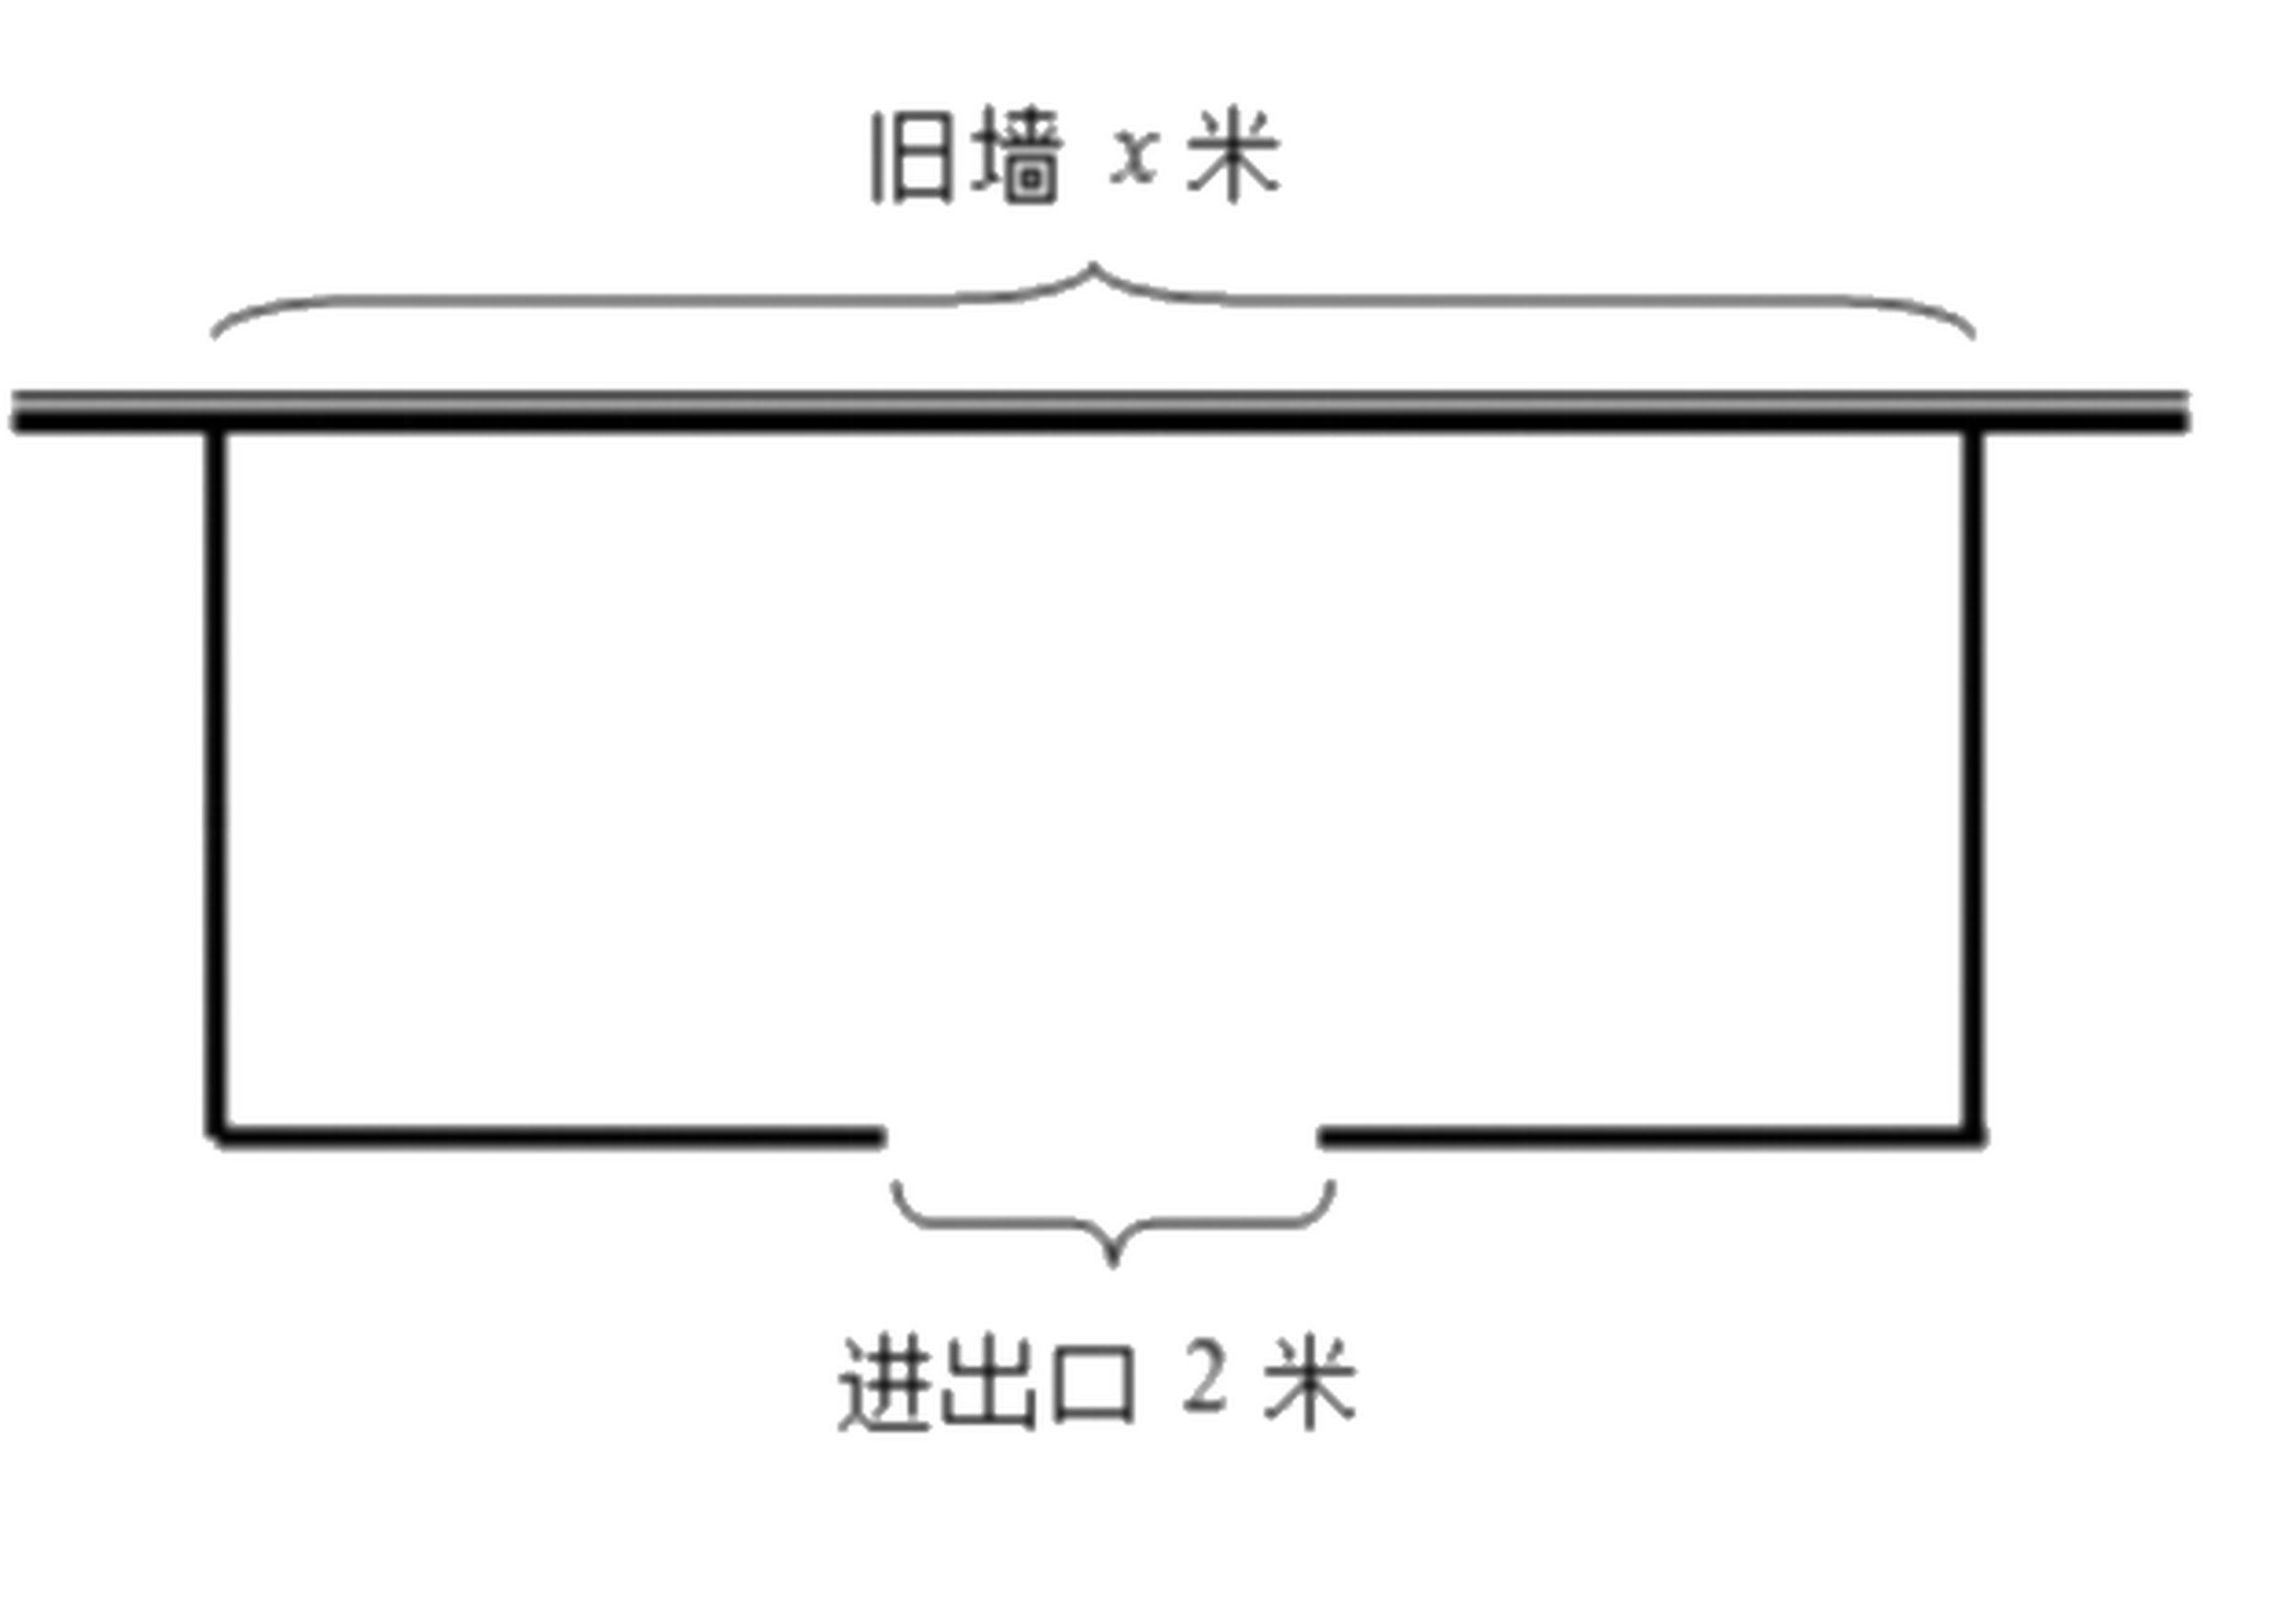
\includegraphics[width=0.60\textwidth]{figures/gao144_q17.png}
\end{center}

(1) 写出总费用 $y$ 关于 $x$ 的表达式;

(2) 试确定 $x$，使修建此矩形场地围墙的总费用最小，并求出最小总费用.

\ifanswer
\solbegin
\step{(1) 设矩形的另一边长为 $a$ 米，}
\step{则 $y=45x+180(x-2)+180\times2a=225x+360a-360$，}
\step{由已知 $xa=360$，得 $a=\dfrac{360}{x}$，所以 $y=225x+\dfrac{360^2}{x}-360(x>0)$;}
\step{(2) 因为 $x>0$，所以 $225x+\dfrac{360^2}{x}\geqslant2\sqrt{225x\cdot\dfrac{360^2}{x}}=10800$，}
\step{所以 $y=225x+\dfrac{360^2}{x}-360\geqslant10440$，}
\step{当且仅当 $225x=\dfrac{360^2}{x}$，即 $x=24$ 时取等号，}
\step{所以当 $x=24$ 米时，修建围墙的总费用最小，最小总费用是 10440 元.}
\solend
\fi

\item 已知集合 $A=\{a_1,a_2,\cdots,a_k\}(k\geqslant2)$，其中 $a_i\in\Z(i=1,2,\cdots,k)$. 定义：若对任意的 $x\in A$，必有 $-x\notin A$，则称集合 $A$ 具有性质 $G$. 由 $A$ 中元素可构成两个点集 $P$ 和 $Q$，$P=\{(x,y)\mid x\in A,y\in A,x+y\in A\}$，$Q=\{(x,y)\mid x\in A,y\in A,x-y\in A\}$，其中 $P$ 有 $m$ 个元素，$Q$ 中有 $n$ 个元素.

(1) 已知集合 $K=\{-1,2,3\}$，判断 $K$ 是否具有性质 $G$; 并写出 $K$ 对应的集合 $P$ 和集合 $Q$;

(2) 若集合 $A=\{1,2,3,4,5,6,7,8,9,10\}$，求对应集合 $Q$ 的元素个数; 一般地，若集合 $A$ 具有性质 $G$，且有 $k$ 个元素，猜测对应的集合 $Q$ 的元素最大个数，并说明理由;

(3) 若集合 $A$ 具有性质 $G$，猜测 $m,n$ 的大小并说明理由.

\ifanswer
\solbegin
\step{(1) 因为 $K=\{-1,2,3\},1,-2,-3$ 都不属于集合 $K$，}
\step{所以集合 $K$ 具有性质 $G$，}
\step{对应集合 $P=\{(-1,3),(3,-1)\},Q=\{(2,-1),(2,3)\}$;}
\step{(2) $A=\{1,2,3,4,5,6,7,8,9,10\}$，则对应集合 $Q$ 中的元素为:}
\step{$(2,1),(3,2),\cdots,(9,8),(10,9)$,}
\step{$(3,1),(4,2),\cdots,(9,7),(10,8)$,}
\step{$(4,1),(5,2),\cdots,(9,6),(10,7)$,}
\step{$\cdots$}
\step{$(9,1),(10,2)$,}
\step{$(10,1)$,}
\step{共有 $9+8+7+\cdots+2+1=45$ 个元素，即对应集合 $Q$ 的元素个数 45;}
\step{集合 $A$ 有 $k$ 个元素，猜测对应的集合 $Q$ 的最大个数为 $\dfrac{k^2-k}{2}$. 理由如下:}
\step{由题意得集合 $A$ 的元素构成有序数对 $(a_i,a_j)(i,j\in\N^*,i\leqslant k,j\leqslant k)$，}
\step{共有 $k^2$ 个，因为 $0\notin A$，所以 $(a_i,a_i)\notin Q$，}
\step{又因为 $a\in A$ 时，$-a\notin A$，所以 $(a_i,a_j)\in Q$ 时，$(a_j,a_i)\notin Q$，}
\step{所以集合 $Q$ 的元素个数为 $\dfrac{k^2-k}{2}$ 个，}
\step{(3) 当集合 $A$ 具有性质 $G$ 时，}
\step{①对于 $(a,b)\in P$，由定义得 $a\in A,b\in A,a+b\in A$，}
\step{又因为集合 $A$ 具有性质 $G$，所以 $(a+b,a)\in Q$，}
\step{如果 $(a,b),(c,d)$ 是 $P$ 中的不同元素，}
\step{那么 $a=c,b=d$ 中至少有一个不成立，}
\step{于是 $b=d,a+b=c+d$ 中至少有一个不成立，}
\step{故 $(a+b,b)$ 和 $(c+d,d)$ 也是 $Q$ 中不同的元素，}
\step{可见 $P$ 的元素个数不多于 $Q$ 的元素个数，即 $m\leqslant n$;}
\step{②对于 $(a,b)\in Q$，由定义得 $a\in A,b\in A,a-b\in A$，}
\step{又因为集合 $A$ 具有性质 $G$，则 $(a-b,b)\in P$，}
\step{如果 $(a,b),(c,d)$ 是 $Q$ 中的不同元素，}
\step{那么 $a=c,b=d$ 中至少有一个不成立，}
\step{于是 $b=d,a-b=c-d$ 中至少有一个不成立，}
\step{故 $(a-b,b)$ 和 $(c-d,d)$ 也是 $P$ 中不同的元素，}
\step{可见 $Q$ 的元素个数不多于 $P$ 的元素个数，即 $n\leqslant m$，}
\step{由①②得 $m=n$.}
\solend
\fi

\end{enumerate}

\end{document}
"
%
% ① 原始材料：微信公众号"魔都数学加油站"文章，连载"27学年高一144"，原文标题
% "27学年高一144——2026-2027年上海市风华中学高一上期中"；
% 原文链接：https://mp.weixin.qq.com/s/ylUlbXfudWOYC-jlH3jyjw 。
% 正文为 10 张 PNG 页，题目下印【解析】，为讲评版。
% 各页分辨率：01/02/03/05/06/07/09/10 为 2560×3620，04/08 为 4762×6735。
% 题目、解析均据原图转录；卷面粉红色水印"魔都数学加油站"及公众号页脚未录入。
% 全卷插图情况：Q17 有一幅矩形场地示意图（旧墙 x 米 / 进出口 2 米），从 07 页裁出、
%   去粉色水印去色 4× LANCZOS 放大存 figures/gao144_q17.png；其余 9 页逐页通读
%   确认无题目配图、无表格、亦无"题干写如图而源码漏图"一处。
%
% 卷首标题：原卷印作"2026-2027 年风华中学高一上期中"，年份区间按全稿惯例排 en dash；
% 原卷卷面未印副标题，本稿按同期中卷（高一140／141／143）知识模块口径补出
% "集合与常用逻辑用语、不等式、函数"：集合与逻辑见 Q3、Q7、Q9、Q10、Q12、Q16、Q18，
% 不等式见 Q6、Q11、Q13、Q14、Q15、Q17，函数见 Q4、Q5、Q8、Q9。
%
% 题号体例：本卷共 16 题——一、填空题 3—10（8 题）、二、选择题 11—13（3 题）、
% 三、解答题 14—18（5 题）。三节分别 \setcounter{enumi}{2}／{10}／{13}。
% 原卷从第 3 题起、无第 1、2 题，本稿保留原题号；全卷无附加题节。
%
% ② 与原卷的排版差异：
%   ① 原文从第 3 题起，本稿保留原题号；共 16 题三节；
%   ② 原卷 15 题题下印【解析】，唯 Q11 未印【解析】、只把答案"（ BD ）"直接印在
%      题干括号内（放大 04 页 A/B 选项与 05 页 C/D 选项衔接处确认，见 ⑤）；
%      按 高一128／94／106／140 成例：Q11 试卷版括号留空 \mbox{（\quad）}、
%      答案版另提 \ans{$BD$}、不补造原卷没有的解析；其余 15 题印【解析】、
%      括号内一律留空、不另提 \ans{}（Q12 选 C、Q13 选 B 在解析末句"故选 …"）；
%      答案版【答案】/【解析】标记数 = 16（1 个 \ans + 15 个 \solbegin）= 全卷题数；
%      正文 Q11 对应处另有 % 注；
%   ③ 原卷卷面未印副标题，本稿按知识模块口径补出；
%   ④ 原卷填空横线按全稿惯例排 \blankline[4.4em]；选择题括号排 \mbox{（\quad）}，
%      选项段前按惯例加 \keepwithprev；解答题不留作答区、不加 \anspace
%      （原卷为讲评版，与 129／131／132／133／136／140／141／143 同）；
%   ⑤ 数集：Q9 题干与解析"a,b∈R"、Q12 题干"U=R"、Q15 题干"x,y∈R"原卷印
%      斜体或黑板粗体 R，Q18 题干"a_i∈Z"印黑板粗体 Z、Q18 解析"i,j∈N*"印
%      黑板粗体 N，按全稿惯例统一改 \R／\Z／\N^*；绝对值排 \lvert…\rvert，
%      集合描述竖线排 \mid；不等号按全稿惯例排 \leqslant／\geqslant；
%      补集照原卷上划线排 \overline{A}／\overline{B}；空集记号 \varnothing；
%   ⑥ 子题标号 (1)(2)(3) 原卷印半角括号，照录；圈数字 ①② 在正文（文本模式）
%      按原卷照录（Q15、Q18 解析），未进数学式；数学式内半角逗号照录
%      （Q12 解析"$A=(1,2),B=(0,6)$"、Q18 解析"$(a_i,a_j)(i,j\in\N^*,i\leqslant k,j\leqslant k)$"、
%      Q15 解析"$x=1,y=-1$"、Q18 解析"$a=c,b=d$"等，为全稿惯例、非笔误）；
%      全卷行末西文句点照录为 ASCII `.`；行中全角逗号／顿号照录；
%      Q18 解析集合描述中的"或"用 \text{ 或 } 置于数学式内；
%   ⑦ 题干中的中文弯引号按原卷照录（Q3 的" x∈A "／" x∈B "与 Q15 (2) 的命题
%      引号，含引号内空格），注释内一律 ASCII 引号；
%   ⑧ Q17 配图：题干写"如图所示"，配图居中排在题干之后、子问之前，三版都出；
%      在 Q17 \item 之前加 \needvspace{10cm} 把"题干＋图"整块推走。Q17 是
%      "三、解答题"节内第 4 题（非节首题），故守卫放在 \item 之前而非 \bigsec
%      之前不会让节标题孤落页末（B 类）；三版切页审计均"合计异常：无"；
%   ⑨ 跨页续印按题合并：Q3 在 01 页；Q4/5/6 在 01 页（Q6 解析续到 02 页顶）；
%      Q7/8/9 在 02 页（Q9 题干跨 02→03）；Q10 在 03 页、解析跨 03→04（很长，
%      按余数分组 A₁/A₂/A₃）；Q11 在 04 页（"二、选择题"节标题也在 04 页下部）、
%      Q12/13 在 05 页（"三、解答题"标题在 05 页下部）；Q14 在 05 页末、解析在 06 页；
%      Q15/16 在 06 页（Q16 续到 07 页）；Q17 在 07 页；Q18 在 08 页、解析跨
%      08/09/10 页（性质 G 压轴，3 问，很长）；本稿按题连排，不丢行、不并折行；
%   ⑩ Q8 解析"法一：""法二："两处标签经放大 02 页逐字确认原卷均印红色
%      （见 ⑤）；按全稿惯例（高一53 成例）不引入红色、均照录为黑体着色
%      \stepm{法一：}{…}／\stepm{法二：}{…}，不改 common.sty；
%      文件头在此注明原卷为红色；
%   ⑪ "图像／图象"逐处核：全卷未出现"图像"或"图象"字样，无统一问题；
%   ⑫ \left…\right 不得拆到不同 $…$ 组；cases 块整体算一个印刷行；
%      Q4 分式与 8×(-3/4) 同一 $…$ 组，Q13 的 \left(\frac1x+\frac2y\right) 同理。
%
% ③ 行数复核：一条 \step／\stepm 行 = 原卷解析的一个印刷行，cases 块作一个印刷行计。
%   逐题数（含 \stepm）：Q3：3；Q4：1；Q5：1；Q6：5；Q7：4；Q8：8（6 \step
%   ＋ 2 \stepm，法一/法二标签各占 1 行）；Q9：6；Q10：23；Q11：0（原卷无解析，
%   答案另提 \ans{$BD$}）；Q12：5；Q13：3；Q14：5；Q15：8；Q16：7；Q17：7；
%   Q18：32。合计 116 条 \step ＋ 2 条 \stepm ＝ 118 个印刷行，与原卷逐题相等。
%   全卷 15 题设 \solbegin…\solend ＋ Q11 一处 \ans{}，答案版【答案】/【解析】
%   标记数 = 16 = 全卷题数。
%
% ④ 判别式／子集符号结论（逐处放大原图照录、不得统一）：
%   判别式全卷 2 处，逐页放大扫过 10 页确认（Q4 为分式指数化简、不含判别式）：
%     · Q9【解析】"所以 △=a^2-4b=0" 原卷印细线、扁等边三角（宽≈高、笔画细，
%       放大见 /tmp/gao144fh/z_q9_tri.png、z_tri_Q9.png），照录 \triangle；
%     · Q15 (2)【解析】cases 块"Δ=(a-2)^2-4(a-2)≤0" 原卷印等腰偏高、粗笔画
%       三角（高>宽，放大见 z_q15_tri.png、z_tri_Q15.png），照录 \Delta；
%   两形不同、全卷混用，逐处照录不统一（参照 高一142 头注④口径）。
%   子集符号全卷 4 处，逐处放大核：
%     · Q3 解析"所以 B⊆A"、Q16 (1) 解析"所以 B⊆A" 原卷均印带下划线的 ⊆
%       （z_q3_symbol.png、z_q16_subset2.png），照录 \subseteq；
%     · Q12 选项 B"$\overline{A}\subset B$" 原卷印单线 ⊂（z_q12_opts2.png），
%       照录 \subset；Q12 解析"$\overline{A}=(-\infty,1]\cup[2,+\infty)\not\subset B$"
%       原卷印单线带斜杠 ⊄（z_q12_notsym3.png），照录 \not\subset；
%   \subset 与 \subseteq 混用，逐处照录不统一。补集照原卷上划线 \overline{A}／
%   \overline{B}，空集 \varnothing，数集 \R／\Z／\N^* 归一见 ② ⑤。
%
% ⑤ 存疑／特殊体例（主会话逐处放大原图复核确认，照录未改，正文对应处另有 % 注）：
%   1. 第 11 题原卷把答案"（ BD ）"直接印在题干括号内、题下未印【解析】
%      （放大 04 页 A/B 选项与 05 页 C/D 选项衔接处确认：05 页顶 C/D 选项后
%      直接接第 12 题）。按 高一128／94／106／140 成例括号留空、另提
%      \ans{$BD$}，不补造解析（不编造）。
%   2. 第 10 题题干"集合 $S$ 为集合 $M=\{1,2,3,4,\cdots,2026\}$，的子集"在
%      集括号与"的子集"之间原卷多印一个全角逗号（放大 03 页确认），
%      按存疑照录未删，正文对应处另有 % 注。
%   3. 第 8 题解析"法一：""法二："两处原卷均印红色（放大 02 页逐字确认），
%      按全稿惯例不引入红色、两处均照录为黑体着色 \stepm（见 ② ⑩）。
%   全卷除此 3 条外未发现其它笔误／自相矛盾处。
%
% ⑥ 跨页续印按题合并说明：见 ② ⑨。
%
\documentclass[a4paper,11pt]{article}
\usepackage{common}

\begin{document}

\examtitlest[3]{2026--2027 年风华中学高一上期中}{集合与常用逻辑用语、不等式、函数}

\bigsec{一、填空题}

\begin{enumerate}
\setcounter{enumi}{2}

\item $A=\{x\mid x>4\}$，$B=\{x\mid x>a\}$，若命题 “ $x\in A$ ” 是命题 “ $x\in B$ ” 的必要条件，则 $a$ 的取值范围是\blankline[4.4em].

\ifanswer
\solbegin
\step{因为 “ $x\in A$ ” 是命题 “ $x\in B$ ” 的必要条件，所以 $B\subseteq A$，}% 子集符号原卷印带下划线 $\subseteq$，照录
\step{因为 $A=\{x\mid x>4\}$，$B=\{x\mid x>a\}$，所以 $a\geqslant4$，}
\step{所以 $a$ 的取值范围是 $\{a\mid a\geqslant4\}$.}
\solend
\fi

\item 已知 $a>0,b>0$，化简式子：$\dfrac{8a^{\frac34}b^3}{\left(a^{\frac16}b^{\frac32}\right)\left(-\dfrac43 a^{\frac1{12}}b^{\frac12}\right)}=$\blankline[4.4em].

\ifanswer
\solbegin
\step{$\dfrac{8a^{\frac34}b^3}{\left(a^{\frac16}b^{\frac32}\right)\left(-\dfrac43 a^{\frac1{12}}b^{\frac12}\right)}=8\times\left(-\dfrac34\right)a^{\frac34-\frac16-\frac1{12}}b^{3-\frac32-\frac12}=-6a^{\frac12}b=-6b\sqrt a$.}
\solend
\fi

\item 已知 $\lg2=a$，$\lg3=b$，则 $\log_5 6=$\blankline[4.4em]（结果用 $a,b$ 表示）.

\ifanswer
\solbegin
\step{$\log_5 6=\dfrac{\lg6}{\lg5}=\dfrac{\lg2+\lg3}{1-\lg2}=\dfrac{a+b}{1-a}$.}
\solend
\fi

\item 若关于 $x$ 的不等式 $ax>b$ 的解集为 $(-\infty,2)$，则不等式 $bx+a>0$ 的解集为\blankline[4.4em].

\ifanswer
\solbegin
\step{因为不等式 $ax>b$ 的解集为 $(-\infty,2)$，所以 $a<0$，}
\step{所以由不等式解得 $x<\dfrac ba$，所以 $\dfrac ba=2$，即 $b=2a$，}
\step{代入不等式 $bx+a>0$，得 $2ax+a>0$，}
\step{因为 $a<0$，所以不等式化为 $2x+1<0$，解得 $x<-\dfrac12$，}
\step{故不等式的解集为 $\left(-\infty,-\dfrac12\right)$.}
\solend
\fi

\item 如果集合 $A=\{x\mid x^2-4x\leqslant0\}$，$B=\{x\mid x^2+ax+b\leqslant0\}$，$A\cap B=\{x\mid3\leqslant x\leqslant4\}$，$A\cup B=\{x\mid0\leqslant x\leqslant5\}$，则 $a+b=$\blankline[4.4em].

\ifanswer
\solbegin
\step{由题意得 $A=\{x\mid x^2-4x\leqslant0\}=[0,4]$，}
\step{又因为 $A\cap B=\{x\mid3\leqslant x\leqslant4\}$，$A\cup B=\{x\mid0\leqslant x\leqslant5\}$，}
\step{所以 $B=\{x\mid3\leqslant x\leqslant5\}$，即方程 $x^2+ax+b=0$ 的两根为 $3,5$，}
\step{由韦达定理得 $\begin{cases}3+5=-a\\3\times5=b\end{cases}$，解得 $a=-8$，$b=15$，所以 $a+b=15-8=7$.}
\solend
\fi

% 第 8 题：原卷"法一：""法二："两处标签均印红色（8× 放大确认）；按交办口径
% "法一"用普通 \step、"法二："排 \stepm（加粗着色、不引红色），见头注 ② ⑩／⑤
\item 若关于 $x$ 的方程 $\lvert x-1\rvert+\lvert\pi-x\rvert=\pi-1$ 的解集为\blankline[4.4em].

\ifanswer
\solbegin
\stepm{法一：}{因为 $\lvert x-1\rvert+\lvert\pi-x\rvert=\begin{cases}x-1+x-\pi,x\geqslant\pi\\\pi-1,1<x<\pi\\1-x+\pi-x,x\leqslant1\end{cases}=\begin{cases}2x-1-\pi,x\geqslant\pi\\\pi-1,1<x<\pi\\1+\pi-2x,x\leqslant1\end{cases}$.}
\step{当 $x\geqslant\pi$ 时，令 $2x-1-\pi=\pi-1$，得 $x=\pi$；}
\step{当 $1<x<\pi$ 时，$\lvert x-1\rvert+\lvert\pi-x\rvert=\pi-1$ 恒成立；}
\step{当 $x\leqslant1$ 时，令 $1+\pi-2x=\pi-1$，得 $x=1$.}
\step{综上所述，方程 $\lvert x-1\rvert+\lvert\pi-x\rvert=\pi-1$ 的解集为 $[1,\pi]$.}
\stepm{法二：}{因为 $\lvert x-1\rvert+\lvert\pi-x\rvert\geqslant\lvert x-1+\pi-x\rvert=\pi-1$，}
\step{当且仅当 $(x-1)(\pi-x)\geqslant0$ 时取等号，}
\step{故方程 $\lvert x-1\rvert+\lvert\pi-x\rvert=\pi-1$ 的解集为 $[1,\pi]$.}
\solend
\fi

% 第 9 题：题干跨 02→03 页；解析判别式原卷印细线扁等边三角 $\triangle$，照录
\item 已知函数 $f(x)=x^2+ax+b(a,b\in\R)$ 和 $x$ 轴有且只有一个交点，若关于 $x$ 的不等式 $f(x)<c$ 的解集为 $(m,m+6)$，则 $c=$\blankline[4.4em].

\ifanswer
\solbegin
\step{因为函数 $f(x)=x^2+ax+b(a,b\in\R)$ 和 $x$ 轴有且只有一个交点，}
\step{所以 $\triangle=a^2-4b=0$，即 $b=\dfrac{a^2}{4}$，}% 判别式原卷印扁等边三角 $\triangle$，照录
\step{不等式 $f(x)<c$ 的解集为 $(m,m+6)$，}
\step{即 $x^2+ax+\dfrac{a^2}{4}-c<0$ 的解集为 $(m,m+6)$，}
\step{所以方程 $x^2+ax+\dfrac{a^2}{4}-c=0$ 的两个根为 $x_1=m$，$x_2=m+6$，}
\step{所以 $\begin{cases}x_1+x_2=2m+6=-a\\x_1x_2=m(m+6)=\dfrac{a^2}{4}-c\end{cases}$，消去 $m$ 得 $\dfrac{a^2}{4}-9=\dfrac{a^2}{4}-c$，解得 $c=9$.}
\solend
\fi

% 第 10 题：原卷题干在集括号与"的子集"之间多印一个全角逗号，照录未改（存疑，见头注 ⑤）
\item 已知集合 $S$ 为集合 $M=\{1,2,3,4,\cdots,2026\}$，的子集，并且集合 $S$ 中任意两个元素之和不能被 3 整除，则集合 $S$ 中元素个数的最大值为\blankline[4.4em].

\ifanswer
\solbegin
\step{对于集合 $M=\{1,2,3,4,\cdots,2026\}$，}
\step{所有被 3 除余数为 0 的元素组成的集合为 $A_3=\{3,6,9,\cdots,2025\}$，}
\step{元素个数为 675;}
\step{所有被 3 除余数为 1 的元素组成的集合为 $A_1=\{1,4,7,\cdots,2026\}$，}
\step{元素个数为 676;}
\step{所有被 3 除余数为 2 的元素组成的集合为 $A_2=\{2,5,8,\cdots,2024\}$，}
\step{元素个数为 675;}
\step{集合 $S$ 中任意两个元素之和不能被 3 整除，}
\step{若两个元素分别来自 $A_1$ 和 $A_2$，则两数之和除以 3 的余数为 $1+2=3\equiv0$，}
\step{即和能被 3 整除，}
\step{所以 $S$ 不能同时包含 $A_1$ 和 $A_2$ 中的元素，}
\step{即 $S$ 最多只能选取 $A_1$、$A_2$ 一个集合中的全部元素;}
\step{若两个元素都来自 $A_3$，则两数之和除以 3 的余数为 $0+0=0$，即和能被 3 整除，}
\step{所以 $S$ 中最多包含 $A_3$ 中的 1 个元素;}
\step{对 $A_1$ 内的任意两个元素，其和除以 3 的余数为 $1+1=2$，不能被 3 整除;}
\step{$A_1$ 中元素与 $A_3$ 中元素的和除以 3 余数为 $1+0=1$，不能被 3 整除，}
\step{所以 $A_1$ 的全部元素与 $A_3$ 中的任意 1 个元素的组合满足题意;}
\step{对 $A_2$ 内的任意两个元素，其和除以 3 的余数为 $2+2=4\equiv1$，不能被 3 整除;}
\step{$A_2$ 中元素与 $A_3$ 中元素的和除以 3 的余数为 $2+0=2$，不能被 3 整除，}
\step{所以 $A_2$ 的全部元素与 $A_3$ 中任意 1 个元素的组合也满足题意.}
\step{故若选取 $A_2$ 全部元素加 1 个 $A_3$ 元素，总个数为 $675+1=676$;}
\step{选取 $A_1$ 全部元素加 1 个 $A_3$ 元素，总个数为 $676+1=677$;}
\step{所以集合 $S$ 中元素个数的最大值为 677.}
\solend
\fi

\end{enumerate}

\bigsec{二、选择题}

\begin{enumerate}
\setcounter{enumi}{10}

% 第 11 题：原卷把答案"（ BD ）"直接印在题干括号内、题下无【解析】（放大 04 页 A/B 选项
% 与 05 页 C/D 选项衔接处确认）。按 高一128／94／106／140 成例：试卷版括号留空、
% 答案版另提 \ans{$BD$}、不补造原卷没有的解析（不编造）。
\item 已知实数 $a,b$，下列四个不等式中正确的是\mbox{（\quad）}

\keepwithprev
A. $a+\dfrac1a\geqslant2$\qquad B. $\sqrt{a^2+2}+\dfrac{1}{\sqrt{a^2+2}}\geqslant2$

C. $\dfrac{a+b}{2}\leqslant\sqrt{ab}$\qquad D. $a^2+b^2\geqslant2ab$

\ifanswer
\ans{$BD$}
\fi

\item 若全集 $U=\R$，$A=\{x\mid x^2-3x+2<0\}$，$B=\{x\mid0<x<6\}$，则\mbox{（\quad）}

\keepwithprev
A. $A\cap B=B$\qquad B. $\overline{A}\subset B$\qquad C. $A\cap\overline{B}=\varnothing$\qquad D. $A\cup B=A$

\ifanswer
\solbegin
\step{由 $x^2-3x+2<0$，则 $A=(1,2),B=(0,6)$，所以 $A\cap B=(1,2)=A,A$ 错误;}
\step{$\overline{A}=(-\infty,1]\cup[2,+\infty)\not\subset B$，$B$ 错误;}
\step{$\overline{B}=(-\infty,0]\cup[6,+\infty)$，所以 $A\cap\overline{B}=\varnothing,C$ 正确;}
\step{$A\cup B=(0,6)\ne A,D$ 错误.}
\step{故选 $C$.}
\solend
\fi

\item 已知正数 $x$、$y$ 满足 $\dfrac1x+\dfrac2y=1$，不等式 $3x+2y-1>m$ 恒成立，则实数 $m$ 的取值范围是\mbox{（\quad）}

\keepwithprev
A. $(-\infty,4+6\sqrt2)$\qquad B. $(-\infty,6+4\sqrt3)$\qquad C. $(6+4\sqrt2,+\infty)$\qquad D. $(8+4\sqrt3,+\infty)$

\ifanswer
\solbegin
\step{$3x+2y=(3x+2y)\left(\dfrac1x+\dfrac2y\right)=7+\dfrac{6x}{y}+\dfrac{2y}{x}\geqslant7+2\sqrt{\dfrac{6x}{y}\cdot\dfrac{2y}{x}}=7+4\sqrt3$，}
\step{当且仅当 $\dfrac{6x}{y}=\dfrac{2y}{x}$，即 $y=\sqrt3x=\sqrt3+2$ 时取等号，}
\step{故要使原式成立，只需 $m<6+4\sqrt3$. 故选 $B$.}
\solend
\fi

\end{enumerate}

\bigsec{三、解答题}

\begin{enumerate}
\setcounter{enumi}{13}

\item 解关于 $x$ 的不等式：

(1) $x^2-2\lvert x\rvert-3>0$；

(2) $\dfrac{2x-1}{x+2}<1$.

\ifanswer
\solbegin
\step{(1) 原不等式等价于 $(\lvert x\rvert-3)(\lvert x\rvert+1)>0$，}
\step{$\lvert x\rvert+1>0$，故 $\lvert x\rvert>3$，解得 $x<-3$ 或 $x>3$，}
\step{故不等式的解集为 $(-\infty,-3)\cup(3,+\infty)$.}
\step{(2) 已知 $\dfrac{2x-1}{x+2}<1$，则 $\dfrac{2x-1}{x+2}-1<0$，即 $\dfrac{x-3}{x+2}<0$，}
\step{等价于 $(x-3)(x+2)<0$，解得 $-2<x<3$，故不等式的解集为 $(-2,3)$.}
\solend
\fi

\item (1) 已知 $x,y\in\R$，比较 $x^2+y^2$ 与 $2x-2y-2$ 的大小.

(2) “不等式 $(a-2)x^2+(a-2)x+1\geqslant0$ 对一切实数恒成立” 是假命题，求实数 $a$ 的取值范围.

\ifanswer
\solbegin
\step{(1) $x^2+y^2-(2x-2y-2)=x^2+y^2-2x+2y+2=(x-1)^2+(y+1)^2\geqslant0$，}
\step{故 $x^2+y^2\geqslant2x-2y-2$，当且仅当 $x=1,y=-1$ 时取等号.}
\step{(2) 先求命题 “$(a-2)x^2+(a-2)x+1\geqslant0$ 对一切实数恒成立” 为真，}
\step{①当 $a-2=0$ 时，即 $a=2$，不等式化为 $1\geqslant0$，成立，符合条件，}
\step{②当 $a-2\ne0$ 时，则 $\begin{cases}a-2>0\\\Delta=(a-2)^2-4(a-2)\leqslant0\end{cases}$，解得 $2<a\leqslant6$，}% 判别式原卷印等腰偏高三角 $\Delta$，照录
\step{综上①②，命题为真时 $2\leqslant a\leqslant6$，}
\step{该命题为假命题，则 $a<2$ 或 $a>6$，}
\step{所以实数 $a$ 的取值范围是 $(-\infty,2)\cup(6,+\infty)$.}
\solend
\fi

\item 设集合 $A=\{x\mid-1\leqslant x\leqslant2\}$，$B=\{x\mid m-1<x<2m+1\}$.

(1) 若 $A\cup B=A$，求实数 $m$ 的取值范围;

(2) 若 $B\cap\overline{A}$ 中只有一个整数 $-2$，求实数 $m$ 的取值范围.

\ifanswer
\solbegin
\step{(1) 因为 $A\cup B=A$，所以 $B\subseteq A$，}% 子集符号原卷印带下划线 $\subseteq$，照录
\step{当 $B=\varnothing$ 时，有 $m-1\geqslant2m+1$，解得 $m\leqslant-2$；}
\step{当 $B\ne\varnothing$ 时，有 $\begin{cases}m-1<2m+1\\m-1\geqslant-1\\2m+1\leqslant2\end{cases}$，解得 $0\leqslant m\leqslant\dfrac12$，}
\step{所以实数 $m$ 的取值范围是 $(-\infty,-2]\cup\left[0,\dfrac12\right]$;}
\step{(2) 由集合 $A=\{x\mid-1\leqslant x\leqslant2\}$，得 $\overline{A}=\{x\mid x<-1\text{ 或 }x>2\}$，}
\step{若 $B\cap\overline{A}$ 中只有一个整数 $-2$，则 $B\ne\varnothing$，且满足 $\begin{cases}m-1<2m+1\\-3\leqslant m-1<-2\\-2<2m+1\leqslant3\end{cases}$}
\step{解得 $-\dfrac32<m<-1$，所以实数 $m$ 的取值范围是 $\left(-\dfrac32,-1\right)$.}
\solend
\fi

% 第 17 题配图是"题干＋图"整块；守卫放在 \item 之前（Q17 非节首题，不会让节标题孤落页末）
\needvspace{10cm}
\item 现要围建一个面积为 360 平方米的矩形场地，要求矩形场地的一面利用旧墙（利用旧墙需维修），其它三面围墙要新建，在旧墙的对面的新墙上要留一个宽度为 2 米的进出口，如图所示，已知旧墙的维修费用为 45 元/米，新墙的造价为 180 元/米，设利用的旧墙的长度为 $x$ 米，工程总造价为 $y$（单位：元）.

\begin{center}
% 矩形场地示意图取自 07 页右侧，去粉色水印、去色、4× LANCZOS 放大
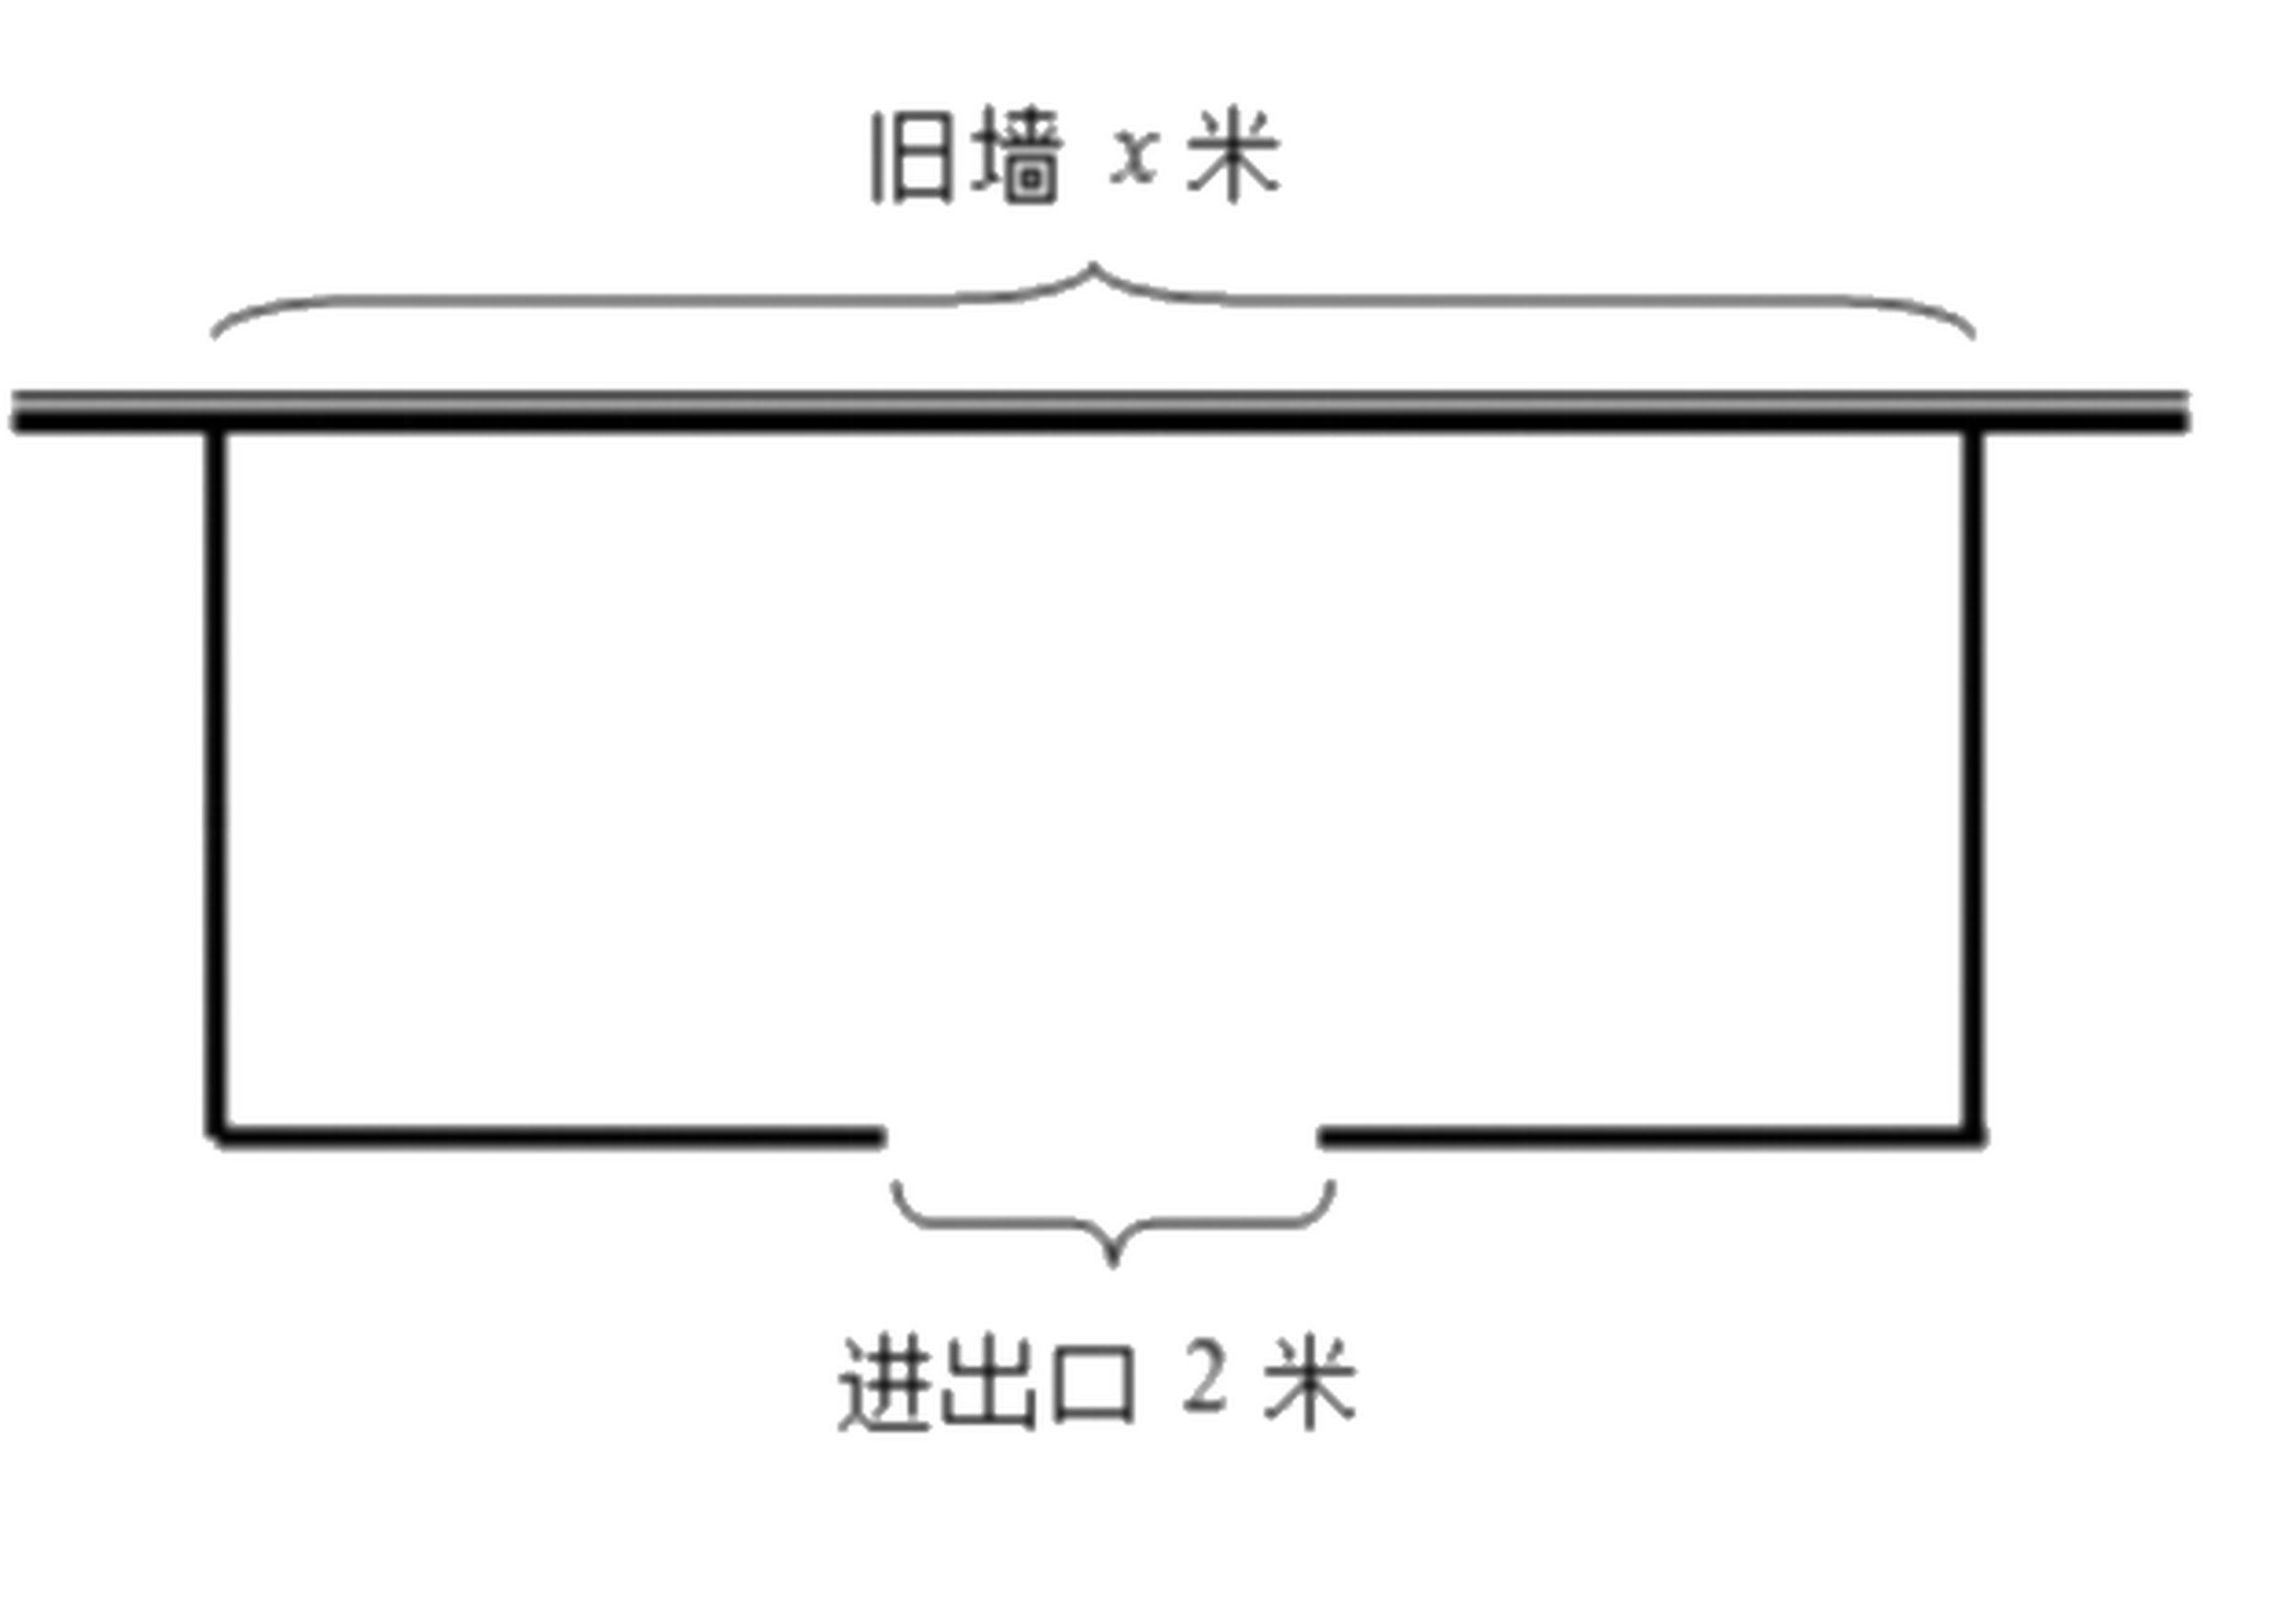
\includegraphics[width=0.60\textwidth]{figures/gao144_q17.png}
\end{center}

(1) 写出总费用 $y$ 关于 $x$ 的表达式;

(2) 试确定 $x$，使修建此矩形场地围墙的总费用最小，并求出最小总费用.

\ifanswer
\solbegin
\step{(1) 设矩形的另一边长为 $a$ 米，}
\step{则 $y=45x+180(x-2)+180\times2a=225x+360a-360$，}
\step{由已知 $xa=360$，得 $a=\dfrac{360}{x}$，所以 $y=225x+\dfrac{360^2}{x}-360(x>0)$;}
\step{(2) 因为 $x>0$，所以 $225x+\dfrac{360^2}{x}\geqslant2\sqrt{225x\cdot\dfrac{360^2}{x}}=10800$，}
\step{所以 $y=225x+\dfrac{360^2}{x}-360\geqslant10440$，}
\step{当且仅当 $225x=\dfrac{360^2}{x}$，即 $x=24$ 时取等号，}
\step{所以当 $x=24$ 米时，修建围墙的总费用最小，最小总费用是 10440 元.}
\solend
\fi

\item 已知集合 $A=\{a_1,a_2,\cdots,a_k\}(k\geqslant2)$，其中 $a_i\in\Z(i=1,2,\cdots,k)$. 定义：若对任意的 $x\in A$，必有 $-x\notin A$，则称集合 $A$ 具有性质 $G$. 由 $A$ 中元素可构成两个点集 $P$ 和 $Q$，$P=\{(x,y)\mid x\in A,y\in A,x+y\in A\}$，$Q=\{(x,y)\mid x\in A,y\in A,x-y\in A\}$，其中 $P$ 有 $m$ 个元素，$Q$ 中有 $n$ 个元素.

(1) 已知集合 $K=\{-1,2,3\}$，判断 $K$ 是否具有性质 $G$; 并写出 $K$ 对应的集合 $P$ 和集合 $Q$;

(2) 若集合 $A=\{1,2,3,4,5,6,7,8,9,10\}$，求对应集合 $Q$ 的元素个数; 一般地，若集合 $A$ 具有性质 $G$，且有 $k$ 个元素，猜测对应的集合 $Q$ 的元素最大个数，并说明理由;

(3) 若集合 $A$ 具有性质 $G$，猜测 $m,n$ 的大小并说明理由.

\ifanswer
\solbegin
\step{(1) 因为 $K=\{-1,2,3\},1,-2,-3$ 都不属于集合 $K$，}
\step{所以集合 $K$ 具有性质 $G$，}
\step{对应集合 $P=\{(-1,3),(3,-1)\},Q=\{(2,-1),(2,3)\}$;}
\step{(2) $A=\{1,2,3,4,5,6,7,8,9,10\}$，则对应集合 $Q$ 中的元素为:}
\step{$(2,1),(3,2),\cdots,(9,8),(10,9)$,}
\step{$(3,1),(4,2),\cdots,(9,7),(10,8)$,}
\step{$(4,1),(5,2),\cdots,(9,6),(10,7)$,}
\step{$\cdots$}
\step{$(9,1),(10,2)$,}
\step{$(10,1)$,}
\step{共有 $9+8+7+\cdots+2+1=45$ 个元素，即对应集合 $Q$ 的元素个数 45;}
\step{集合 $A$ 有 $k$ 个元素，猜测对应的集合 $Q$ 的最大个数为 $\dfrac{k^2-k}{2}$. 理由如下:}
\step{由题意得集合 $A$ 的元素构成有序数对 $(a_i,a_j)(i,j\in\N^*,i\leqslant k,j\leqslant k)$，}
\step{共有 $k^2$ 个，因为 $0\notin A$，所以 $(a_i,a_i)\notin Q$，}
\step{又因为 $a\in A$ 时，$-a\notin A$，所以 $(a_i,a_j)\in Q$ 时，$(a_j,a_i)\notin Q$，}
\step{所以集合 $Q$ 的元素个数为 $\dfrac{k^2-k}{2}$ 个，}
\step{(3) 当集合 $A$ 具有性质 $G$ 时，}
\step{①对于 $(a,b)\in P$，由定义得 $a\in A,b\in A,a+b\in A$，}
\step{又因为集合 $A$ 具有性质 $G$，所以 $(a+b,a)\in Q$，}
\step{如果 $(a,b),(c,d)$ 是 $P$ 中的不同元素，}
\step{那么 $a=c,b=d$ 中至少有一个不成立，}
\step{于是 $b=d,a+b=c+d$ 中至少有一个不成立，}
\step{故 $(a+b,b)$ 和 $(c+d,d)$ 也是 $Q$ 中不同的元素，}
\step{可见 $P$ 的元素个数不多于 $Q$ 的元素个数，即 $m\leqslant n$;}
\step{②对于 $(a,b)\in Q$，由定义得 $a\in A,b\in A,a-b\in A$，}
\step{又因为集合 $A$ 具有性质 $G$，则 $(a-b,b)\in P$，}
\step{如果 $(a,b),(c,d)$ 是 $Q$ 中的不同元素，}
\step{那么 $a=c,b=d$ 中至少有一个不成立，}
\step{于是 $b=d,a-b=c-d$ 中至少有一个不成立，}
\step{故 $(a-b,b)$ 和 $(c-d,d)$ 也是 $P$ 中不同的元素，}
\step{可见 $Q$ 的元素个数不多于 $P$ 的元素个数，即 $n\leqslant m$，}
\step{由①②得 $m=n$.}
\solend
\fi

\end{enumerate}

\end{document}
"
%
% ① 原始材料：微信公众号"魔都数学加油站"文章，连载"27学年高一144"，原文标题
% "27学年高一144——2026-2027年上海市风华中学高一上期中"；
% 原文链接：https://mp.weixin.qq.com/s/ylUlbXfudWOYC-jlH3jyjw 。
% 正文为 10 张 PNG 页，题目下印【解析】，为讲评版。
% 各页分辨率：01/02/03/05/06/07/09/10 为 2560×3620，04/08 为 4762×6735。
% 题目、解析均据原图转录；卷面粉红色水印"魔都数学加油站"及公众号页脚未录入。
% 全卷插图情况：Q17 有一幅矩形场地示意图（旧墙 x 米 / 进出口 2 米），从 07 页裁出、
%   去粉色水印去色 4× LANCZOS 放大存 figures/gao144_q17.png；其余 9 页逐页通读
%   确认无题目配图、无表格、亦无"题干写如图而源码漏图"一处。
%
% 卷首标题：原卷印作"2026-2027 年风华中学高一上期中"，年份区间按全稿惯例排 en dash；
% 原卷卷面未印副标题，本稿按同期中卷（高一140／141／143）知识模块口径补出
% "集合与常用逻辑用语、不等式、函数"：集合与逻辑见 Q3、Q7、Q9、Q10、Q12、Q16、Q18，
% 不等式见 Q6、Q11、Q13、Q14、Q15、Q17，函数见 Q4、Q5、Q8、Q9。
%
% 题号体例：本卷共 16 题——一、填空题 3—10（8 题）、二、选择题 11—13（3 题）、
% 三、解答题 14—18（5 题）。三节分别 \setcounter{enumi}{2}／{10}／{13}。
% 原卷从第 3 题起、无第 1、2 题，本稿保留原题号；全卷无附加题节。
%
% ② 与原卷的排版差异：
%   ① 原文从第 3 题起，本稿保留原题号；共 16 题三节；
%   ② 原卷 15 题题下印【解析】，唯 Q11 未印【解析】、只把答案"（ BD ）"直接印在
%      题干括号内（放大 04 页 A/B 选项与 05 页 C/D 选项衔接处确认，见 ⑤）；
%      按 高一128／94／106／140 成例：Q11 试卷版括号留空 \mbox{（\quad）}、
%      答案版另提 \ans{$BD$}、不补造原卷没有的解析；其余 15 题印【解析】、
%      括号内一律留空、不另提 \ans{}（Q12 选 C、Q13 选 B 在解析末句"故选 …"）；
%      答案版【答案】/【解析】标记数 = 16（1 个 \ans + 15 个 \solbegin）= 全卷题数；
%      正文 Q11 对应处另有 % 注；
%   ③ 原卷卷面未印副标题，本稿按知识模块口径补出；
%   ④ 原卷填空横线按全稿惯例排 \blankline[4.4em]；选择题括号排 \mbox{（\quad）}，
%      选项段前按惯例加 \keepwithprev；解答题不留作答区、不加 \anspace
%      （原卷为讲评版，与 129／131／132／133／136／140／141／143 同）；
%   ⑤ 数集：Q9 题干与解析"a,b∈R"、Q12 题干"U=R"、Q15 题干"x,y∈R"原卷印
%      斜体或黑板粗体 R，Q18 题干"a_i∈Z"印黑板粗体 Z、Q18 解析"i,j∈N*"印
%      黑板粗体 N，按全稿惯例统一改 \R／\Z／\N^*；绝对值排 \lvert…\rvert，
%      集合描述竖线排 \mid；不等号按全稿惯例排 \leqslant／\geqslant；
%      补集照原卷上划线排 \overline{A}／\overline{B}；空集记号 \varnothing；
%   ⑥ 子题标号 (1)(2)(3) 原卷印半角括号，照录；圈数字 ①② 在正文（文本模式）
%      按原卷照录（Q15、Q18 解析），未进数学式；数学式内半角逗号照录
%      （Q12 解析"$A=(1,2),B=(0,6)$"、Q18 解析"$(a_i,a_j)(i,j\in\N^*,i\leqslant k,j\leqslant k)$"、
%      Q15 解析"$x=1,y=-1$"、Q18 解析"$a=c,b=d$"等，为全稿惯例、非笔误）；
%      全卷行末西文句点照录为 ASCII `.`；行中全角逗号／顿号照录；
%      Q18 解析集合描述中的"或"用 \text{ 或 } 置于数学式内；
%   ⑦ 题干中的中文弯引号按原卷照录（Q3 的" x∈A "／" x∈B "与 Q15 (2) 的命题
%      引号，含引号内空格），注释内一律 ASCII 引号；
%   ⑧ Q17 配图：题干写"如图所示"，配图居中排在题干之后、子问之前，三版都出；
%      在 Q17 \item 之前加 \needvspace{10cm} 把"题干＋图"整块推走。Q17 是
%      "三、解答题"节内第 4 题（非节首题），故守卫放在 \item 之前而非 \bigsec
%      之前不会让节标题孤落页末（B 类）；三版切页审计均"合计异常：无"；
%   ⑨ 跨页续印按题合并：Q3 在 01 页；Q4/5/6 在 01 页（Q6 解析续到 02 页顶）；
%      Q7/8/9 在 02 页（Q9 题干跨 02→03）；Q10 在 03 页、解析跨 03→04（很长，
%      按余数分组 A₁/A₂/A₃）；Q11 在 04 页（"二、选择题"节标题也在 04 页下部）、
%      Q12/13 在 05 页（"三、解答题"标题在 05 页下部）；Q14 在 05 页末、解析在 06 页；
%      Q15/16 在 06 页（Q16 续到 07 页）；Q17 在 07 页；Q18 在 08 页、解析跨
%      08/09/10 页（性质 G 压轴，3 问，很长）；本稿按题连排，不丢行、不并折行；
%   ⑩ Q8 解析"法一：""法二："两处标签经放大 02 页逐字确认原卷均印红色
%      （见 ⑤）；按全稿惯例（高一53 成例）不引入红色、均照录为黑体着色
%      \stepm{法一：}{…}／\stepm{法二：}{…}，不改 common.sty；
%      文件头在此注明原卷为红色；
%   ⑪ "图像／图象"逐处核：全卷未出现"图像"或"图象"字样，无统一问题；
%   ⑫ \left…\right 不得拆到不同 $…$ 组；cases 块整体算一个印刷行；
%      Q4 分式与 8×(-3/4) 同一 $…$ 组，Q13 的 \left(\frac1x+\frac2y\right) 同理。
%
% ③ 行数复核：一条 \step／\stepm 行 = 原卷解析的一个印刷行，cases 块作一个印刷行计。
%   逐题数（含 \stepm）：Q3：3；Q4：1；Q5：1；Q6：5；Q7：4；Q8：8（6 \step
%   ＋ 2 \stepm，法一/法二标签各占 1 行）；Q9：6；Q10：23；Q11：0（原卷无解析，
%   答案另提 \ans{$BD$}）；Q12：5；Q13：3；Q14：5；Q15：8；Q16：7；Q17：7；
%   Q18：32。合计 116 条 \step ＋ 2 条 \stepm ＝ 118 个印刷行，与原卷逐题相等。
%   全卷 15 题设 \solbegin…\solend ＋ Q11 一处 \ans{}，答案版【答案】/【解析】
%   标记数 = 16 = 全卷题数。
%
% ④ 判别式／子集符号结论（逐处放大原图照录、不得统一）：
%   判别式全卷 2 处，逐页放大扫过 10 页确认（Q4 为分式指数化简、不含判别式）：
%     · Q9【解析】"所以 △=a^2-4b=0" 原卷印细线、扁等边三角（宽≈高、笔画细，
%       放大见 /tmp/gao144fh/z_q9_tri.png、z_tri_Q9.png），照录 \triangle；
%     · Q15 (2)【解析】cases 块"Δ=(a-2)^2-4(a-2)≤0" 原卷印等腰偏高、粗笔画
%       三角（高>宽，放大见 z_q15_tri.png、z_tri_Q15.png），照录 \Delta；
%   两形不同、全卷混用，逐处照录不统一（参照 高一142 头注④口径）。
%   子集符号全卷 4 处，逐处放大核：
%     · Q3 解析"所以 B⊆A"、Q16 (1) 解析"所以 B⊆A" 原卷均印带下划线的 ⊆
%       （z_q3_symbol.png、z_q16_subset2.png），照录 \subseteq；
%     · Q12 选项 B"$\overline{A}\subset B$" 原卷印单线 ⊂（z_q12_opts2.png），
%       照录 \subset；Q12 解析"$\overline{A}=(-\infty,1]\cup[2,+\infty)\not\subset B$"
%       原卷印单线带斜杠 ⊄（z_q12_notsym3.png），照录 \not\subset；
%   \subset 与 \subseteq 混用，逐处照录不统一。补集照原卷上划线 \overline{A}／
%   \overline{B}，空集 \varnothing，数集 \R／\Z／\N^* 归一见 ② ⑤。
%
% ⑤ 存疑／特殊体例（主会话逐处放大原图复核确认，照录未改，正文对应处另有 % 注）：
%   1. 第 11 题原卷把答案"（ BD ）"直接印在题干括号内、题下未印【解析】
%      （放大 04 页 A/B 选项与 05 页 C/D 选项衔接处确认：05 页顶 C/D 选项后
%      直接接第 12 题）。按 高一128／94／106／140 成例括号留空、另提
%      \ans{$BD$}，不补造解析（不编造）。
%   2. 第 10 题题干"集合 $S$ 为集合 $M=\{1,2,3,4,\cdots,2026\}$，的子集"在
%      集括号与"的子集"之间原卷多印一个全角逗号（放大 03 页确认），
%      按存疑照录未删，正文对应处另有 % 注。
%   3. 第 8 题解析"法一：""法二："两处原卷均印红色（放大 02 页逐字确认），
%      按全稿惯例不引入红色、两处均照录为黑体着色 \stepm（见 ② ⑩）。
%   全卷除此 3 条外未发现其它笔误／自相矛盾处。
%
% ⑥ 跨页续印按题合并说明：见 ② ⑨。
%
\documentclass[a4paper,11pt]{article}
\usepackage{common}

\begin{document}

\examtitlest[3]{2026--2027 年风华中学高一上期中}{集合与常用逻辑用语、不等式、函数}

\bigsec{一、填空题}

\begin{enumerate}
\setcounter{enumi}{2}

\item $A=\{x\mid x>4\}$，$B=\{x\mid x>a\}$，若命题 “ $x\in A$ ” 是命题 “ $x\in B$ ” 的必要条件，则 $a$ 的取值范围是\blankline[4.4em].

\ifanswer
\solbegin
\step{因为 “ $x\in A$ ” 是命题 “ $x\in B$ ” 的必要条件，所以 $B\subseteq A$，}% 子集符号原卷印带下划线 $\subseteq$，照录
\step{因为 $A=\{x\mid x>4\}$，$B=\{x\mid x>a\}$，所以 $a\geqslant4$，}
\step{所以 $a$ 的取值范围是 $\{a\mid a\geqslant4\}$.}
\solend
\fi

\item 已知 $a>0,b>0$，化简式子：$\dfrac{8a^{\frac34}b^3}{\left(a^{\frac16}b^{\frac32}\right)\left(-\dfrac43 a^{\frac1{12}}b^{\frac12}\right)}=$\blankline[4.4em].

\ifanswer
\solbegin
\step{$\dfrac{8a^{\frac34}b^3}{\left(a^{\frac16}b^{\frac32}\right)\left(-\dfrac43 a^{\frac1{12}}b^{\frac12}\right)}=8\times\left(-\dfrac34\right)a^{\frac34-\frac16-\frac1{12}}b^{3-\frac32-\frac12}=-6a^{\frac12}b=-6b\sqrt a$.}
\solend
\fi

\item 已知 $\lg2=a$，$\lg3=b$，则 $\log_5 6=$\blankline[4.4em]（结果用 $a,b$ 表示）.

\ifanswer
\solbegin
\step{$\log_5 6=\dfrac{\lg6}{\lg5}=\dfrac{\lg2+\lg3}{1-\lg2}=\dfrac{a+b}{1-a}$.}
\solend
\fi

\item 若关于 $x$ 的不等式 $ax>b$ 的解集为 $(-\infty,2)$，则不等式 $bx+a>0$ 的解集为\blankline[4.4em].

\ifanswer
\solbegin
\step{因为不等式 $ax>b$ 的解集为 $(-\infty,2)$，所以 $a<0$，}
\step{所以由不等式解得 $x<\dfrac ba$，所以 $\dfrac ba=2$，即 $b=2a$，}
\step{代入不等式 $bx+a>0$，得 $2ax+a>0$，}
\step{因为 $a<0$，所以不等式化为 $2x+1<0$，解得 $x<-\dfrac12$，}
\step{故不等式的解集为 $\left(-\infty,-\dfrac12\right)$.}
\solend
\fi

\item 如果集合 $A=\{x\mid x^2-4x\leqslant0\}$，$B=\{x\mid x^2+ax+b\leqslant0\}$，$A\cap B=\{x\mid3\leqslant x\leqslant4\}$，$A\cup B=\{x\mid0\leqslant x\leqslant5\}$，则 $a+b=$\blankline[4.4em].

\ifanswer
\solbegin
\step{由题意得 $A=\{x\mid x^2-4x\leqslant0\}=[0,4]$，}
\step{又因为 $A\cap B=\{x\mid3\leqslant x\leqslant4\}$，$A\cup B=\{x\mid0\leqslant x\leqslant5\}$，}
\step{所以 $B=\{x\mid3\leqslant x\leqslant5\}$，即方程 $x^2+ax+b=0$ 的两根为 $3,5$，}
\step{由韦达定理得 $\begin{cases}3+5=-a\\3\times5=b\end{cases}$，解得 $a=-8$，$b=15$，所以 $a+b=15-8=7$.}
\solend
\fi

% 第 8 题：原卷"法一：""法二："两处标签均印红色（8× 放大确认）；按交办口径
% "法一"用普通 \step、"法二："排 \stepm（加粗着色、不引红色），见头注 ② ⑩／⑤
\item 若关于 $x$ 的方程 $\lvert x-1\rvert+\lvert\pi-x\rvert=\pi-1$ 的解集为\blankline[4.4em].

\ifanswer
\solbegin
\stepm{法一：}{因为 $\lvert x-1\rvert+\lvert\pi-x\rvert=\begin{cases}x-1+x-\pi,x\geqslant\pi\\\pi-1,1<x<\pi\\1-x+\pi-x,x\leqslant1\end{cases}=\begin{cases}2x-1-\pi,x\geqslant\pi\\\pi-1,1<x<\pi\\1+\pi-2x,x\leqslant1\end{cases}$.}
\step{当 $x\geqslant\pi$ 时，令 $2x-1-\pi=\pi-1$，得 $x=\pi$；}
\step{当 $1<x<\pi$ 时，$\lvert x-1\rvert+\lvert\pi-x\rvert=\pi-1$ 恒成立；}
\step{当 $x\leqslant1$ 时，令 $1+\pi-2x=\pi-1$，得 $x=1$.}
\step{综上所述，方程 $\lvert x-1\rvert+\lvert\pi-x\rvert=\pi-1$ 的解集为 $[1,\pi]$.}
\stepm{法二：}{因为 $\lvert x-1\rvert+\lvert\pi-x\rvert\geqslant\lvert x-1+\pi-x\rvert=\pi-1$，}
\step{当且仅当 $(x-1)(\pi-x)\geqslant0$ 时取等号，}
\step{故方程 $\lvert x-1\rvert+\lvert\pi-x\rvert=\pi-1$ 的解集为 $[1,\pi]$.}
\solend
\fi

% 第 9 题：题干跨 02→03 页；解析判别式原卷印细线扁等边三角 $\triangle$，照录
\item 已知函数 $f(x)=x^2+ax+b(a,b\in\R)$ 和 $x$ 轴有且只有一个交点，若关于 $x$ 的不等式 $f(x)<c$ 的解集为 $(m,m+6)$，则 $c=$\blankline[4.4em].

\ifanswer
\solbegin
\step{因为函数 $f(x)=x^2+ax+b(a,b\in\R)$ 和 $x$ 轴有且只有一个交点，}
\step{所以 $\triangle=a^2-4b=0$，即 $b=\dfrac{a^2}{4}$，}% 判别式原卷印扁等边三角 $\triangle$，照录
\step{不等式 $f(x)<c$ 的解集为 $(m,m+6)$，}
\step{即 $x^2+ax+\dfrac{a^2}{4}-c<0$ 的解集为 $(m,m+6)$，}
\step{所以方程 $x^2+ax+\dfrac{a^2}{4}-c=0$ 的两个根为 $x_1=m$，$x_2=m+6$，}
\step{所以 $\begin{cases}x_1+x_2=2m+6=-a\\x_1x_2=m(m+6)=\dfrac{a^2}{4}-c\end{cases}$，消去 $m$ 得 $\dfrac{a^2}{4}-9=\dfrac{a^2}{4}-c$，解得 $c=9$.}
\solend
\fi

% 第 10 题：原卷题干在集括号与"的子集"之间多印一个全角逗号，照录未改（存疑，见头注 ⑤）
\item 已知集合 $S$ 为集合 $M=\{1,2,3,4,\cdots,2026\}$，的子集，并且集合 $S$ 中任意两个元素之和不能被 3 整除，则集合 $S$ 中元素个数的最大值为\blankline[4.4em].

\ifanswer
\solbegin
\step{对于集合 $M=\{1,2,3,4,\cdots,2026\}$，}
\step{所有被 3 除余数为 0 的元素组成的集合为 $A_3=\{3,6,9,\cdots,2025\}$，}
\step{元素个数为 675;}
\step{所有被 3 除余数为 1 的元素组成的集合为 $A_1=\{1,4,7,\cdots,2026\}$，}
\step{元素个数为 676;}
\step{所有被 3 除余数为 2 的元素组成的集合为 $A_2=\{2,5,8,\cdots,2024\}$，}
\step{元素个数为 675;}
\step{集合 $S$ 中任意两个元素之和不能被 3 整除，}
\step{若两个元素分别来自 $A_1$ 和 $A_2$，则两数之和除以 3 的余数为 $1+2=3\equiv0$，}
\step{即和能被 3 整除，}
\step{所以 $S$ 不能同时包含 $A_1$ 和 $A_2$ 中的元素，}
\step{即 $S$ 最多只能选取 $A_1$、$A_2$ 一个集合中的全部元素;}
\step{若两个元素都来自 $A_3$，则两数之和除以 3 的余数为 $0+0=0$，即和能被 3 整除，}
\step{所以 $S$ 中最多包含 $A_3$ 中的 1 个元素;}
\step{对 $A_1$ 内的任意两个元素，其和除以 3 的余数为 $1+1=2$，不能被 3 整除;}
\step{$A_1$ 中元素与 $A_3$ 中元素的和除以 3 余数为 $1+0=1$，不能被 3 整除，}
\step{所以 $A_1$ 的全部元素与 $A_3$ 中的任意 1 个元素的组合满足题意;}
\step{对 $A_2$ 内的任意两个元素，其和除以 3 的余数为 $2+2=4\equiv1$，不能被 3 整除;}
\step{$A_2$ 中元素与 $A_3$ 中元素的和除以 3 的余数为 $2+0=2$，不能被 3 整除，}
\step{所以 $A_2$ 的全部元素与 $A_3$ 中任意 1 个元素的组合也满足题意.}
\step{故若选取 $A_2$ 全部元素加 1 个 $A_3$ 元素，总个数为 $675+1=676$;}
\step{选取 $A_1$ 全部元素加 1 个 $A_3$ 元素，总个数为 $676+1=677$;}
\step{所以集合 $S$ 中元素个数的最大值为 677.}
\solend
\fi

\end{enumerate}

\bigsec{二、选择题}

\begin{enumerate}
\setcounter{enumi}{10}

% 第 11 题：原卷把答案"（ BD ）"直接印在题干括号内、题下无【解析】（放大 04 页 A/B 选项
% 与 05 页 C/D 选项衔接处确认）。按 高一128／94／106／140 成例：试卷版括号留空、
% 答案版另提 \ans{$BD$}、不补造原卷没有的解析（不编造）。
\item 已知实数 $a,b$，下列四个不等式中正确的是\mbox{（\quad）}

\keepwithprev
A. $a+\dfrac1a\geqslant2$\qquad B. $\sqrt{a^2+2}+\dfrac{1}{\sqrt{a^2+2}}\geqslant2$

C. $\dfrac{a+b}{2}\leqslant\sqrt{ab}$\qquad D. $a^2+b^2\geqslant2ab$

\ifanswer
\ans{$BD$}
\fi

\item 若全集 $U=\R$，$A=\{x\mid x^2-3x+2<0\}$，$B=\{x\mid0<x<6\}$，则\mbox{（\quad）}

\keepwithprev
A. $A\cap B=B$\qquad B. $\overline{A}\subset B$\qquad C. $A\cap\overline{B}=\varnothing$\qquad D. $A\cup B=A$

\ifanswer
\solbegin
\step{由 $x^2-3x+2<0$，则 $A=(1,2),B=(0,6)$，所以 $A\cap B=(1,2)=A,A$ 错误;}
\step{$\overline{A}=(-\infty,1]\cup[2,+\infty)\not\subset B$，$B$ 错误;}
\step{$\overline{B}=(-\infty,0]\cup[6,+\infty)$，所以 $A\cap\overline{B}=\varnothing,C$ 正确;}
\step{$A\cup B=(0,6)\ne A,D$ 错误.}
\step{故选 $C$.}
\solend
\fi

\item 已知正数 $x$、$y$ 满足 $\dfrac1x+\dfrac2y=1$，不等式 $3x+2y-1>m$ 恒成立，则实数 $m$ 的取值范围是\mbox{（\quad）}

\keepwithprev
A. $(-\infty,4+6\sqrt2)$\qquad B. $(-\infty,6+4\sqrt3)$\qquad C. $(6+4\sqrt2,+\infty)$\qquad D. $(8+4\sqrt3,+\infty)$

\ifanswer
\solbegin
\step{$3x+2y=(3x+2y)\left(\dfrac1x+\dfrac2y\right)=7+\dfrac{6x}{y}+\dfrac{2y}{x}\geqslant7+2\sqrt{\dfrac{6x}{y}\cdot\dfrac{2y}{x}}=7+4\sqrt3$，}
\step{当且仅当 $\dfrac{6x}{y}=\dfrac{2y}{x}$，即 $y=\sqrt3x=\sqrt3+2$ 时取等号，}
\step{故要使原式成立，只需 $m<6+4\sqrt3$. 故选 $B$.}
\solend
\fi

\end{enumerate}

\bigsec{三、解答题}

\begin{enumerate}
\setcounter{enumi}{13}

\item 解关于 $x$ 的不等式：

(1) $x^2-2\lvert x\rvert-3>0$；

(2) $\dfrac{2x-1}{x+2}<1$.

\ifanswer
\solbegin
\step{(1) 原不等式等价于 $(\lvert x\rvert-3)(\lvert x\rvert+1)>0$，}
\step{$\lvert x\rvert+1>0$，故 $\lvert x\rvert>3$，解得 $x<-3$ 或 $x>3$，}
\step{故不等式的解集为 $(-\infty,-3)\cup(3,+\infty)$.}
\step{(2) 已知 $\dfrac{2x-1}{x+2}<1$，则 $\dfrac{2x-1}{x+2}-1<0$，即 $\dfrac{x-3}{x+2}<0$，}
\step{等价于 $(x-3)(x+2)<0$，解得 $-2<x<3$，故不等式的解集为 $(-2,3)$.}
\solend
\fi

\item (1) 已知 $x,y\in\R$，比较 $x^2+y^2$ 与 $2x-2y-2$ 的大小.

(2) “不等式 $(a-2)x^2+(a-2)x+1\geqslant0$ 对一切实数恒成立” 是假命题，求实数 $a$ 的取值范围.

\ifanswer
\solbegin
\step{(1) $x^2+y^2-(2x-2y-2)=x^2+y^2-2x+2y+2=(x-1)^2+(y+1)^2\geqslant0$，}
\step{故 $x^2+y^2\geqslant2x-2y-2$，当且仅当 $x=1,y=-1$ 时取等号.}
\step{(2) 先求命题 “$(a-2)x^2+(a-2)x+1\geqslant0$ 对一切实数恒成立” 为真，}
\step{①当 $a-2=0$ 时，即 $a=2$，不等式化为 $1\geqslant0$，成立，符合条件，}
\step{②当 $a-2\ne0$ 时，则 $\begin{cases}a-2>0\\\Delta=(a-2)^2-4(a-2)\leqslant0\end{cases}$，解得 $2<a\leqslant6$，}% 判别式原卷印等腰偏高三角 $\Delta$，照录
\step{综上①②，命题为真时 $2\leqslant a\leqslant6$，}
\step{该命题为假命题，则 $a<2$ 或 $a>6$，}
\step{所以实数 $a$ 的取值范围是 $(-\infty,2)\cup(6,+\infty)$.}
\solend
\fi

\item 设集合 $A=\{x\mid-1\leqslant x\leqslant2\}$，$B=\{x\mid m-1<x<2m+1\}$.

(1) 若 $A\cup B=A$，求实数 $m$ 的取值范围;

(2) 若 $B\cap\overline{A}$ 中只有一个整数 $-2$，求实数 $m$ 的取值范围.

\ifanswer
\solbegin
\step{(1) 因为 $A\cup B=A$，所以 $B\subseteq A$，}% 子集符号原卷印带下划线 $\subseteq$，照录
\step{当 $B=\varnothing$ 时，有 $m-1\geqslant2m+1$，解得 $m\leqslant-2$；}
\step{当 $B\ne\varnothing$ 时，有 $\begin{cases}m-1<2m+1\\m-1\geqslant-1\\2m+1\leqslant2\end{cases}$，解得 $0\leqslant m\leqslant\dfrac12$，}
\step{所以实数 $m$ 的取值范围是 $(-\infty,-2]\cup\left[0,\dfrac12\right]$;}
\step{(2) 由集合 $A=\{x\mid-1\leqslant x\leqslant2\}$，得 $\overline{A}=\{x\mid x<-1\text{ 或 }x>2\}$，}
\step{若 $B\cap\overline{A}$ 中只有一个整数 $-2$，则 $B\ne\varnothing$，且满足 $\begin{cases}m-1<2m+1\\-3\leqslant m-1<-2\\-2<2m+1\leqslant3\end{cases}$}
\step{解得 $-\dfrac32<m<-1$，所以实数 $m$ 的取值范围是 $\left(-\dfrac32,-1\right)$.}
\solend
\fi

% 第 17 题配图是"题干＋图"整块；守卫放在 \item 之前（Q17 非节首题，不会让节标题孤落页末）
\needvspace{10cm}
\item 现要围建一个面积为 360 平方米的矩形场地，要求矩形场地的一面利用旧墙（利用旧墙需维修），其它三面围墙要新建，在旧墙的对面的新墙上要留一个宽度为 2 米的进出口，如图所示，已知旧墙的维修费用为 45 元/米，新墙的造价为 180 元/米，设利用的旧墙的长度为 $x$ 米，工程总造价为 $y$（单位：元）.

\begin{center}
% 矩形场地示意图取自 07 页右侧，去粉色水印、去色、4× LANCZOS 放大
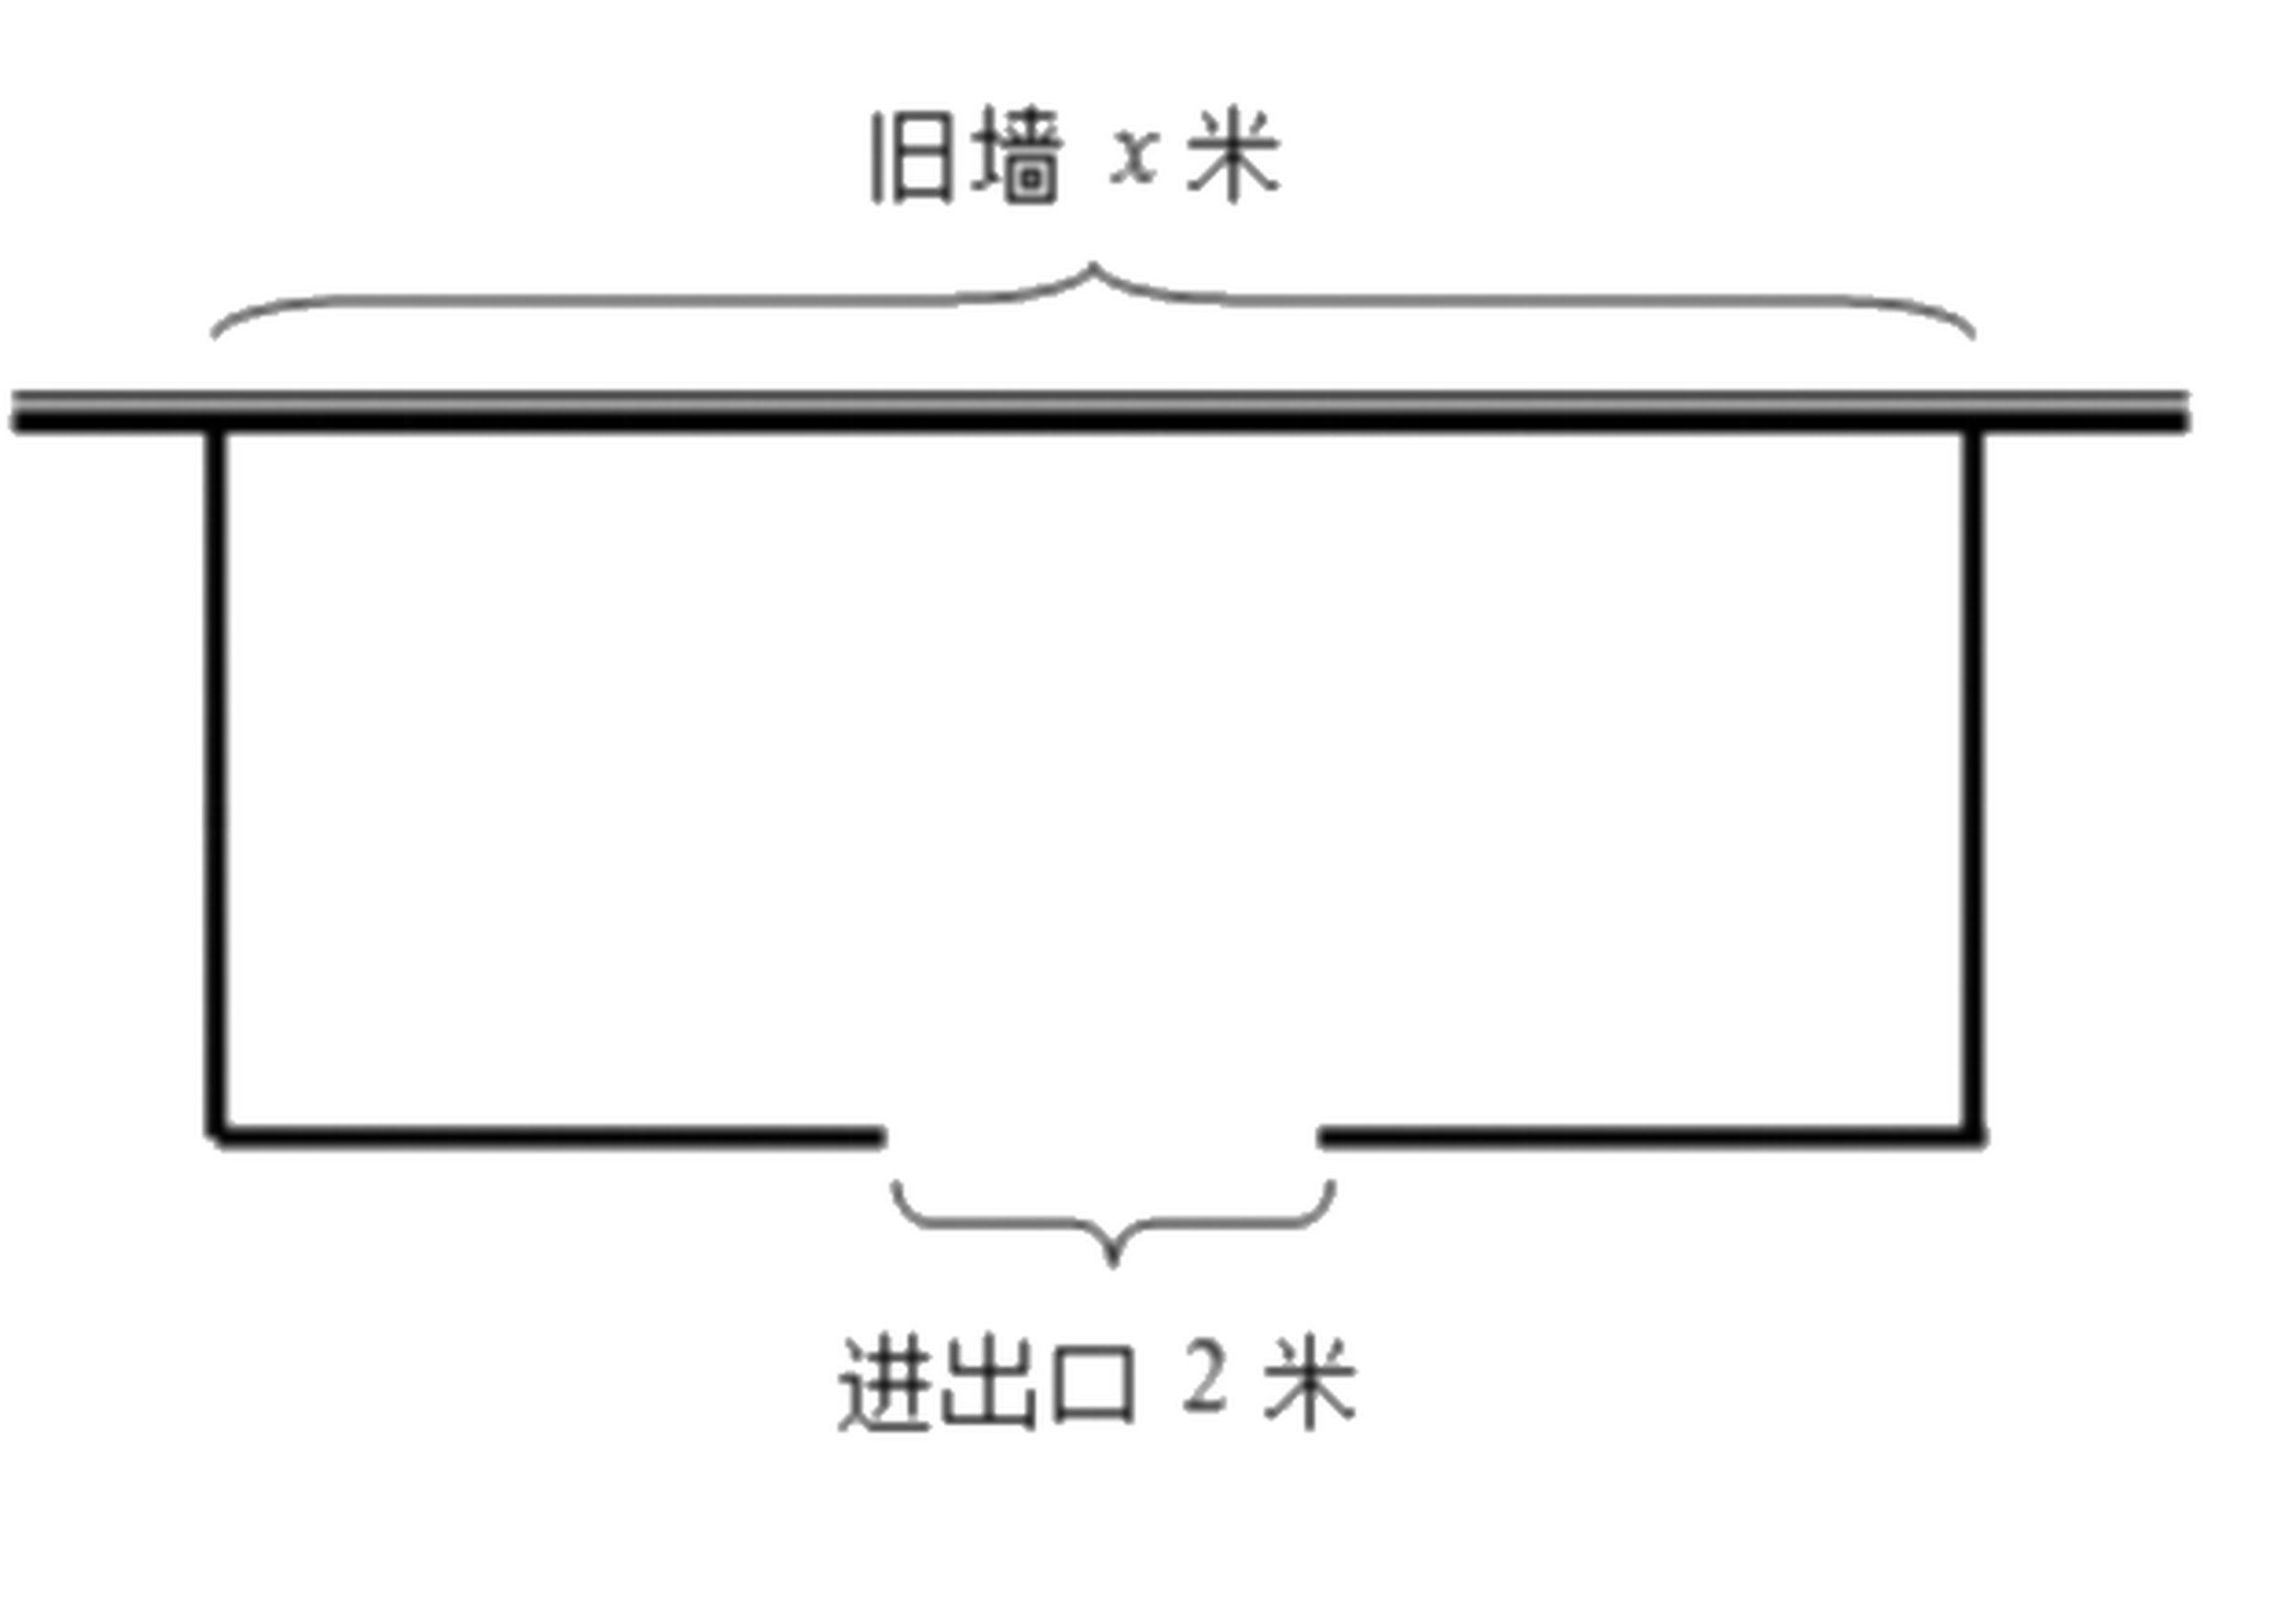
\includegraphics[width=0.60\textwidth]{figures/gao144_q17.png}
\end{center}

(1) 写出总费用 $y$ 关于 $x$ 的表达式;

(2) 试确定 $x$，使修建此矩形场地围墙的总费用最小，并求出最小总费用.

\ifanswer
\solbegin
\step{(1) 设矩形的另一边长为 $a$ 米，}
\step{则 $y=45x+180(x-2)+180\times2a=225x+360a-360$，}
\step{由已知 $xa=360$，得 $a=\dfrac{360}{x}$，所以 $y=225x+\dfrac{360^2}{x}-360(x>0)$;}
\step{(2) 因为 $x>0$，所以 $225x+\dfrac{360^2}{x}\geqslant2\sqrt{225x\cdot\dfrac{360^2}{x}}=10800$，}
\step{所以 $y=225x+\dfrac{360^2}{x}-360\geqslant10440$，}
\step{当且仅当 $225x=\dfrac{360^2}{x}$，即 $x=24$ 时取等号，}
\step{所以当 $x=24$ 米时，修建围墙的总费用最小，最小总费用是 10440 元.}
\solend
\fi

\item 已知集合 $A=\{a_1,a_2,\cdots,a_k\}(k\geqslant2)$，其中 $a_i\in\Z(i=1,2,\cdots,k)$. 定义：若对任意的 $x\in A$，必有 $-x\notin A$，则称集合 $A$ 具有性质 $G$. 由 $A$ 中元素可构成两个点集 $P$ 和 $Q$，$P=\{(x,y)\mid x\in A,y\in A,x+y\in A\}$，$Q=\{(x,y)\mid x\in A,y\in A,x-y\in A\}$，其中 $P$ 有 $m$ 个元素，$Q$ 中有 $n$ 个元素.

(1) 已知集合 $K=\{-1,2,3\}$，判断 $K$ 是否具有性质 $G$; 并写出 $K$ 对应的集合 $P$ 和集合 $Q$;

(2) 若集合 $A=\{1,2,3,4,5,6,7,8,9,10\}$，求对应集合 $Q$ 的元素个数; 一般地，若集合 $A$ 具有性质 $G$，且有 $k$ 个元素，猜测对应的集合 $Q$ 的元素最大个数，并说明理由;

(3) 若集合 $A$ 具有性质 $G$，猜测 $m,n$ 的大小并说明理由.

\ifanswer
\solbegin
\step{(1) 因为 $K=\{-1,2,3\},1,-2,-3$ 都不属于集合 $K$，}
\step{所以集合 $K$ 具有性质 $G$，}
\step{对应集合 $P=\{(-1,3),(3,-1)\},Q=\{(2,-1),(2,3)\}$;}
\step{(2) $A=\{1,2,3,4,5,6,7,8,9,10\}$，则对应集合 $Q$ 中的元素为:}
\step{$(2,1),(3,2),\cdots,(9,8),(10,9)$,}
\step{$(3,1),(4,2),\cdots,(9,7),(10,8)$,}
\step{$(4,1),(5,2),\cdots,(9,6),(10,7)$,}
\step{$\cdots$}
\step{$(9,1),(10,2)$,}
\step{$(10,1)$,}
\step{共有 $9+8+7+\cdots+2+1=45$ 个元素，即对应集合 $Q$ 的元素个数 45;}
\step{集合 $A$ 有 $k$ 个元素，猜测对应的集合 $Q$ 的最大个数为 $\dfrac{k^2-k}{2}$. 理由如下:}
\step{由题意得集合 $A$ 的元素构成有序数对 $(a_i,a_j)(i,j\in\N^*,i\leqslant k,j\leqslant k)$，}
\step{共有 $k^2$ 个，因为 $0\notin A$，所以 $(a_i,a_i)\notin Q$，}
\step{又因为 $a\in A$ 时，$-a\notin A$，所以 $(a_i,a_j)\in Q$ 时，$(a_j,a_i)\notin Q$，}
\step{所以集合 $Q$ 的元素个数为 $\dfrac{k^2-k}{2}$ 个，}
\step{(3) 当集合 $A$ 具有性质 $G$ 时，}
\step{①对于 $(a,b)\in P$，由定义得 $a\in A,b\in A,a+b\in A$，}
\step{又因为集合 $A$ 具有性质 $G$，所以 $(a+b,a)\in Q$，}
\step{如果 $(a,b),(c,d)$ 是 $P$ 中的不同元素，}
\step{那么 $a=c,b=d$ 中至少有一个不成立，}
\step{于是 $b=d,a+b=c+d$ 中至少有一个不成立，}
\step{故 $(a+b,b)$ 和 $(c+d,d)$ 也是 $Q$ 中不同的元素，}
\step{可见 $P$ 的元素个数不多于 $Q$ 的元素个数，即 $m\leqslant n$;}
\step{②对于 $(a,b)\in Q$，由定义得 $a\in A,b\in A,a-b\in A$，}
\step{又因为集合 $A$ 具有性质 $G$，则 $(a-b,b)\in P$，}
\step{如果 $(a,b),(c,d)$ 是 $Q$ 中的不同元素，}
\step{那么 $a=c,b=d$ 中至少有一个不成立，}
\step{于是 $b=d,a-b=c-d$ 中至少有一个不成立，}
\step{故 $(a-b,b)$ 和 $(c-d,d)$ 也是 $P$ 中不同的元素，}
\step{可见 $Q$ 的元素个数不多于 $P$ 的元素个数，即 $n\leqslant m$，}
\step{由①②得 $m=n$.}
\solend
\fi

\end{enumerate}

\end{document}
